% This is a LaTeX thesis template for Monash University.
% to be used with Rmarkdown
% This template was produced by Rob Hyndman
% Version: 6 September 2016

\documentclass{monashthesis}

%%%%%%%%%%%%%%%%%%%%%%%%%%%%%%%%%%%%%%%%%%%%%%%%%%%%%%%%%%%%%%%
% Add any LaTeX packages and other preamble here if required
%%%%%%%%%%%%%%%%%%%%%%%%%%%%%%%%%%%%%%%%%%%%%%%%%%%%%%%%%%%%%%%

\author{Stephanie Rose Kobakian}
\title{New Algorithms For Effectively Visualising Australian Spatio-Temporal Disease Data}
\degrees{B.Comm. and B.Eco., Monash University}
\def\degreetitle{Master of Philosophy (Statistics)}
% Add subject and keywords below
\hypersetup{
     %pdfsubject={The Subject},
     %pdfkeywords={Some Keywords},
     pdfauthor={Stephanie Rose Kobakian},
     pdftitle={New Algorithms For Effectively Visualising Australian Spatio-Temporal Disease Data},
     pdfproducer={Bookdown with LaTeX}
}


\bibliography{thesisrefs}

\begin{document}

\pagenumbering{roman}

\titlepage

{\setstretch{1.2}\sf\tighttoc\doublespacing}

\hypertarget{copyright-notice}{%
\chapter*{Copyright notice}\label{copyright-notice}}
\addcontentsline{toc}{chapter}{Copyright notice}

\textcopyright { } \authorname~(\number\the\year).

I certify that I have made all reasonable efforts to secure copyright permissions for third-party content included in this thesis and have not knowingly added copyright content to my work without the owner's permission.

\newpage

\hypertarget{keywords}{%
\chapter*{Keywords}\label{keywords}}
\addcontentsline{toc}{chapter}{Keywords}

Keywords:
cartogram; choropleth; geospatial statistics; maps; statistics; tile maps; visual inference

\hypertarget{abstract}{%
\chapter*{Abstract}\label{abstract}}
\addcontentsline{toc}{chapter}{Abstract}

Relationships between geographic areas can be communicated using maps. The speed of visual processes allow quick comparisons to be made between neighbouring areas. However, when presenting population-related statistics on the geographic map base, large areas that draw readers' attention can allow too much emphasis to be placed on sparsely populated rural areas.
This problem can dramatically impact the interpretation of statistics across Australia, due to the large difference in the land area when the population is concentrated in a few small areas.

In this thesis a new algorithm for laying out spatial areas into a tessellated hexgon tile is developed. This layout is used to create a new visualisation method for displaying disease data for Australia.
An experiment was conducted that indicates that this visualisation outperforms the traditional choropleth map for communicating disease data.
A software implementation was generated and made publicly available for others to use these techniques. In addition, animation can be used to translate from the choropleth map to the new tessellated hexagon display to help viewers interpret the new display.

\newpage

\hypertarget{list-of-figures}{%
\chapter*{List of Figures}\label{list-of-figures}}
\addcontentsline{toc}{chapter}{List of Figures}

\begin{tabular}{rr>{\raggedright\arraybackslash}p{15cm}}
\toprule
Figure & Caption & Page\\
\midrule
2.1 & A selection of choropleth cancer maps from online atlases that are publicly available. & 16\\
2.2 & Common alternatives to maps, showing the same information for the United States of America. & 26\\
2.3 & Two alternative displays, tile map (left) and geofaceted map (right), showing state age-adjusted rate of incidence for lung and bronchus in the USA. & 30\\
2.4 & Cartograms showing melanoma incidence in Australia. & 31\\
2.5 & Interactive controls of displays in publicly available choropleth cancer maps & 34\\
\addlinespace
2.6 & Two examples of advanced interactivity (and animation) in publicly available choropleth cancer maps. & 35\\
\bottomrule
\end{tabular}

\begin{tabular}{rr>{\raggedright\arraybackslash}p{15cm}}
\toprule
Figure & Caption & Page\\
\midrule
3.1 & The geographic shapes of the Statistical Areas of Tasmania at Level 2. & 44\\
3.2 & Grid points to create a tilegram. & 45\\
3.3 & All possible hexagon locations from the initial grid are shown with blue outlines. & 47\\
3.4 & Filter for grid points within a square, then circular, distance for those closest to the centroid. & 49\\
3.5 & Filter for grid points within the angle from the focal point to the centroid. & 50\\
\addlinespace
3.6 & A complete hexagon tile map of Tasmania & 51\\
3.7 & The Australian Cancer Atlas data has determined the colour of each Statistical Area of Australian at Level 2 & 52\\
3.8 & A choropleth map of the Statistical Areas of Australia at Level 2. & 55\\
3.9 & A hexagon tile map of the Statistical Areas of Australia at Level 2. & 56\\
\bottomrule
\end{tabular}

\begin{tabular}{rr>{\raggedright\arraybackslash}p{15cm}}
\toprule
Figure & Caption & Page\\
\midrule
4.1 & A choropleth map of the smoothed average of liver cancer diagnoses for Australian males. & 60\\
4.2 & A hexagon tile map of the smoothed average of liver cancer diagnoses for Australian males. & 60\\
4.3 & This lineup of twelve hexagon tile map displays contains one map with a real population related structure. & 61\\
4.4 & The experimental design used in the visual inference study. & 62\\
4.5 & The detection rates achieved by participants are contrasted when viewing the four replicates of the three trend models & 64\\
\addlinespace
4.6 & The distribution of the time taken (seconds) to submit a response for each combination of trend, whether the data plot was detected, and type of display, shown using horizontally jittered dotplots. & 65\\
4.7 & The amount of times each level of certainty was chosen by participants when viewing hexagon tile map or choropleth displays. & 66\\
\bottomrule
\end{tabular}

\hypertarget{list-of-tables}{%
\chapter*{List of Tables}\label{list-of-tables}}
\addcontentsline{toc}{chapter}{List of Tables}

\begin{tabular}{rr>{\raggedright\arraybackslash}p{25em}}
\toprule
Figure & Caption & Page\\
\midrule
2.1 & A selection of choropleth cancer maps from online atlases. & 16\\
2.2 & Common measures for reporting cancer information. & 19\\
2.3 & Maps used to present statistics for the United States of America. & 24\\
2.4 & Summary of features and constraints of common mapping methods used to display
cancer statistics. & 32\\
\bottomrule
\end{tabular}

\begin{tabular}{rr>{\raggedright\arraybackslash}p{25em}r}
\toprule
Chapter & Table & Caption & Page\\
\midrule
4 & I (1) & The mean and standard deviation of the rate of detection for each trend model, calculated for the choropleth and hexagon tile map displays. & 64\\
4 & II (2) & The model output for the generalised linear mixed effect model for detection rate. & 65\\
4 & III (3) & The amount of participants that selected each reason for their choice of plot when looking at each trend model shown in Choropleth and Hexagon Tile maps. & 66\\
\bottomrule
\end{tabular}

\hypertarget{list-of-publications}{%
\chapter*{List of Publications}\label{list-of-publications}}
\addcontentsline{toc}{chapter}{List of Publications}

\begin{enumerate}
\def\labelenumi{\arabic{enumi}.}
\tightlist
\item
  The exploration of the literature regarding current practices for visualising spatial data is presented in Chapter \ref{ch:literature} has been submitted to the journal \emph{Annals of Cancer Epidemiology} for publication.
\end{enumerate}

Kobakian S. and Cook, D. and Roberts, J. (2019). Cancer Applications of Choropleth Maps, and the Potential of Cartograms and Alternative Map Displays. Manuscript submitted for publication.

\begin{enumerate}
\def\labelenumi{\arabic{enumi}.}
\setcounter{enumi}{1}
\tightlist
\item
  The discussion of the algorithm documented in Chapter \ref{ch:algorithm} will be submitted to the \emph{Journal of Statistical Software}.
\end{enumerate}

Kobakian S. and Cook, D. (2020). An Algorithm For Spatial Mapping Using a Hexagon Tile Map, With Application to Australian Maps. Manuscript in preparation.

\begin{enumerate}
\def\labelenumi{\arabic{enumi}.}
\setcounter{enumi}{2}
\tightlist
\item
  The details of the experiment to test the alternative hexagon tile map is documented in Chapter \ref{ch:experiment} will be submitted to the \emph{IEEE Transactions of Visualisation and Computer Graphics} under the title ``Comparing the Effectiveness of the Choropleth Map with a Hexagon Tile Map for Communicating Cancer''
\end{enumerate}

Kobakian S. and Cook, D. (2020). Comparing the Effectiveness of the Choropleth Map with a Hexagon Tile Map for Communicating Cancer Manuscript in preparation.

\begin{enumerate}
\def\labelenumi{\arabic{enumi}.}
\setcounter{enumi}{3}
\tightlist
\item
  The code for the algorithm documented in Chapter \ref{ch:algorithm} is currently hosted on \emph{CRAN} as the package sugarbag.
\end{enumerate}

Kobakian, S. and Cook, D. (2019). sugarbag: Create Tessellated Hexagon Maps. \url{https://srkobakian.github.io/sugarbag/}, \url{https://github.com/srkobakian/sugarbag}.

\clearpage\pagenumbering{arabic}\setcounter{page}{0}

\hypertarget{declaration}{%
\chapter*{Declaration}\label{declaration}}
\addcontentsline{toc}{chapter}{Declaration}

I hereby declare that this thesis contains no material which has been accepted for the award of any other degree or diploma at any university or equivalent institution and that, to the best of my knowledge and belief, this thesis contains no material previously published or written by another person, except where due reference is made in the text of the thesis.

This thesis includes three original papers submitted to peer reviewed journals. The core theme of the thesis is spatial visualisations. The ideas, development and writing up of all the papers in the thesis were the principal responsibility of myself, the student, working within the Faculty of Science and Engineering under the supervision of Distinguished Professor Kerrie Mengersen and Dr.~Earl Duncan. It was also created under the supervision of the external supervisor Professor Dianne Cook from Monash University.

The papers in Chapters 2, 3, and 4 have been individually formatted for journal submission however, I have renumbered the pages of the submitted papers for cohesion across this thesis.

\hypertarget{acknowledgements}{%
\chapter*{Acknowledgements}\label{acknowledgements}}
\addcontentsline{toc}{chapter}{Acknowledgements}

This thesis would not be possible without the opportunity provided by Queensland University of Technology, Cancer Council Queensland and the ARC Centre of Excellence for Mathematical \& Statistical Frontiers.

I would like to acknowledge my supervisors for their tireless work in directing, encouraging and supporting this work.

Professor Dianne Cook (Professor, Department of Econometrics and Business Statistics, Monash University) provided constant support, encouragement and recommendations throughout this degree.

Dr Earl Duncan (Research Associate at ARC Centre of Excellence for Mathematical \& Statistical Frontiers, QUT) provided regular time for discussion, editing and commenting throughout this degree.

Professor Kerrie Mengersen (Professor of Statistics, Science and Engineering Faculty, QUT) provided the opportunity to study at Queensland University of Technology, organising and mentoring me through this project.

Working closely with Prof.~Di Cook enabled the rapid development of my research and writing skills.

\hypertarget{cancer-applications-of-choropleth-maps-and-the-potential-of-cartograms-and-alternative-map-displays}{%
\section{Cancer Applications of Choropleth Maps, and the Potential of Cartograms and Alternative Map Displays}\label{cancer-applications-of-choropleth-maps-and-the-potential-of-cartograms-and-alternative-map-displays}}

With my coauthors Prof.~Dianne Cook and Jessie Roberts, I would like to acknowledge Dr Susanna Cramb (Strategic Research Fellow, Institute of Health Biomedical Innovation, Queensland Univeristy of Technology) and Dr Peter Baade (Senior Research Fellow, Cancer Council Queensland) for providing the opportunity and time to discuss alternative map solutions for presentation in the Australian Cancer Atlas.
It was in the development of this online cancer atlas that methods for disease map displays, and visual communication strategies were explored.

\hypertarget{comparing-the-effectiveness-of-the-choropleth-map-with-a-hexagon-tile-map-for-communicating-cancer}{%
\section{Comparing the Effectiveness of the Choropleth Map with a Hexagon Tile Map for Communicating Cancer}\label{comparing-the-effectiveness-of-the-choropleth-map-with-a-hexagon-tile-map-for-communicating-cancer}}

I would like to thank Mitchell O'Hara-Wild was a co-developer of the taipan \autocite{taipan} R package for the web app constructed to collect participant evaluations of lineups.

We are thankful for the NUMBATs (Non-Uniform Monash Business Analytics Team) for participating in the pilot study that helped to assess the experimental design and determine an appropriate sample size for the study.

\hypertarget{r-packages}{%
\section{R packages}\label{r-packages}}

Several \texttt{R} \autocite{R} packages were used to produce this thesis:

\begin{itemize}
\tightlist
\item
  \texttt{absmapsdata} \autocite{ABSmaps}
\item
  \texttt{cartogram} \autocite{cartogram}
\item
  \texttt{cowplot} \autocite{cowplot}
\item
  \texttt{eechidna} \autocite{eechidna}
\item
  \texttt{ggplot2} \autocite{ggplot2}
\item
  \texttt{ggthemes} \autocite{ggthemes}
\item
  \texttt{grid} \autocite{grid}
\item
  \texttt{gstat} \autocite{gstat}
\item
  \texttt{kableExtra} \autocite{kableExtra}.
\item
  \texttt{knitr} \autocite{knitr}
\item
  \texttt{lme4} \autocite{lme4}
\item
  \texttt{nullabor} \autocite{nullabor}
\item
  \texttt{png} \autocite{png}
\item
  \texttt{RColorBrewer} \autocite{RColorBrewer}
\item
  \texttt{rmarkdown} \autocite{rmarkdown}
\item
  \texttt{rticles} \autocite{rticles}
\item
  \texttt{sf} \autocite{sf}
\item
  \texttt{spData} \autocite{spData}
\item
  \texttt{sugarbag} \autocite{sugarbag}
\item
  \texttt{tidyverse} \autocite{tidyverse}
\end{itemize}

\hypertarget{ch:intro}{%
\chapter{Introduction}\label{ch:intro}}

Maps can contribute to the interpretation of spatial distributions of disease occurrence, and help to locate disease clusters. Disease data is commonly aggravated to political areas. privacy is one reason for this and another is the responsibility of the political entity to respond. The typical visualisation for aggregated spatial data is a choropleth map, where areas are coloured according to a numerical value. A choropleth map is the most common display for the presentation of geospatial data.

Choropleth maps do a disservice to the map reader, as the attention of the map user is distributed according to the size of the area. Using a choropleth map to get a broad perspective of Australia can be misleading, when the size of geographical areas misrepresent the spatial distribution of a dataset. This representation is not practical if each area is considered equally important. In Australia, the population is not equally dispersed across the geographic map base.
Instead, the communities are densely populated in the inner city areas, especially around the capital cities. There are several visualisation methods that have been developed to emphasise the population dense areas. These alternatives should be considered when planning the communication of geospatial statistics, as visualisations should be chosen to best represent the spatial distribution. This work is motivated by the Australian Cancer Atlas, which presents the spatial patterns of cancer in Australia. The aim of this thesis is to contribute an algorithm that creates effective visualisations for the communication of geospatial population statistics.

\hypertarget{the-australian-cancer-atlas}{%
\section{The Australian Cancer Atlas}\label{the-australian-cancer-atlas}}

This thesis and it's contributions were motivated by the Australian Cancer Atlas (ACA), an online, interactive web tool for exploring the impact of cancer on Australian communities. The prominent display used by the ACA to present incidence rates or excess death rates is the choropleth map. The set of geographic units shown are the Australian Statistical Areas, at Level 2 (SA2s). There are almost 2,200 individual SA2s.

The choropleth map used in the ACA is familiar to the general public of Australia. It is appropriate to use this map display as users can orient themselves on the map and find the geographic areas relevant to them.
However, when the intention of the map user is to understand the whole spatial distribution, the information derived from the colours displayed on the map can be misleading.
The rural areas in outback Australia are over emphasised, and the densely populated inner city areas are not given enough attention, as they cannot be sen using a choropleth map.

\hypertarget{testing-graphical-displays}{%
\section{Testing graphical displays}\label{testing-graphical-displays}}

Visual inference testing will be used to determine if the communication of population geospatial statistics is more effective when using the new alternative hexagon tile map display.
Buja et al \autocite{GIIV} provide the `lineup' protocol as a formal framework for testing visual statistical methods. The new alternative visualisation method can be tested by implementing this framework.
It takes inspiration from a police lineup.
The lineup protocol can be used to test if the hexagon tile map is effective, a map displaying a real population based distribution can be hidden in a collection of maps that display null distributions \autocite{chowd}.

The `witness' in this regard is the participant recruited from a crowdsource platform.
The visualisation in the lineup that contains a real distribution is considered the `accused'.
It is put in a lineup of innocent displays that do not show a population based distribution.
If the `witness' chooses the `accused' when asked `Which display is the most different?' from the innocent plots, it can be considered that there may be a pattern displayed that is not present in the others.
In this protocol, the null hypothesis can be rejected in favour of the alternative when the `accused' display is chosen to be the most different display in the lineup. The null hypothesis fails to be rejected when it is not selected in the lineup.

\hypertarget{sec:aims}{%
\section{Aims and Objectives}\label{sec:aims}}

This thesis aims to provide a solution to presenting geospatial data regarding populations.
It considers the visualisation methods developed over the past two centuries that shift the focus from the geographic map base.

\begin{enumerate}
\def\labelenumi{\arabic{enumi}.}
\item
  \emph{Devising an Algorithm for creating hexagon tile maps of Australia:} The algorithm will take geospatial areas and create an alternative visualisation of the spatial distribution.
\item
  \emph{Test the effectiveness of the hexagon tile map relative to the choropleth map:} The hexagon tile map produced by the algorithm will be contrasted with the traditional choropleth map, applying the same colour methods to represent the data.
\item
  \emph{Communicating the relationship between the hexmap and choropleth map through animation:} Animations can maximise the benefits of both visualisation methods when communicating to the public. The use of animations may control how people follow a recognisable map of Australia into an alternative visualisation for inference.
\end{enumerate}

\hypertarget{research-contributions}{%
\section{Research Contributions}\label{research-contributions}}

This research contributes a new algorithm for creating hexagon tile map displays. It contributes an R \autocite{R} package which implements the algorithm and allows R users to create their own visualisations.
It presents a case study that contributes to a growing field of visual inference studies. Applying the lineup protocol to spatial data by comparing a choropleth map to a hexagon tile map display.
It also shows how it can be used in practice to effectively communicate population related cancer distributions.

\hypertarget{thesis-structure}{%
\section{Thesis Structure}\label{thesis-structure}}

The thesis is structured as follows: Chapter two contains a literature review.
The literature reviews considers the current peer reviewed literature and published books that explore spatial distributions of cancer across the globe.
It also considers how to evaluate the visualisation methods used for spatial data.

Chapter three explores the algorithm to create hexagon tile maps and the code used to create a small example of Tasmania in Australia.
Chapter four discusses an experiment that uses visual inference. It contains the methods and results that compare the use of a choropleth map and a hexagon tile map.
Chapter five provides a conclusion of the results of the visual inference study and how the hexagon tile map may be used in practice.

\hypertarget{ch:literature}{%
\chapter{Cancer Applications of Choropleth Maps, and the Potential of Cartograms and Alternative Map Displays}\label{ch:literature}}

This literature review chapter provides an overview of the key areas of interest in the literature that are relevant to this thesis. This chapter is organised as follows. Section 1 outlines the traditional spatial mapping technique, the choropleth map, and provides design inspiration using examples of online cancer atlases. Section 2 outlines contemporary mapping approaches, suggested as alternatives to the choropleth. Section 3 compares and critiques these alternative displays in light of the strengths and weaknesses of the choropleth method. section 4 considers how users interact with mapping displays in online cancer atlases, and how map creators can direct the attention of uses through animation. Additionally, the following chapters in this thesis each begin with a section to introduce the specific relevant literature.

This chapter was submitted for publication to the journal \emph{Annals of Cancer Epidemiology} for publication. This was intended for an audience of cancer atlas creators to be inspired by current atlases, and to encourage the pursuit of alternative displays.

\includepdf[pages = {1-}, scale=0.8]{statement-of-contribution_literature.pdf}

\newpage

\hypertarget{abstract-1}{%
\section*{Abstract}\label{abstract-1}}
\addcontentsline{toc}{section}{Abstract}

Cancer atlases communicate cancer statistics over geographic domains, typically with a choropleth map. They subdivide these domains into administrative regions such as countries, states, or suburbs. When communicating human-related statistics, the choropleth has a disadvantage in that it draws attention to sparsely populated rural areas to the neglect of small inner city areas. The smaller geographic areas are important to consider if they are densely populated. Alternative map displays, such as a cartogram or a hexagon tile map, can shift the attention of map users from the large rural areas by decreasing their size on the map display. This means alternative displays can be more effective at accurately communicating spatial patterns across spatial areas. It is recommended that alternative displays are included in cancer atlases. In addition, with the ease of today's technology, user interaction with the displays is encouraged. Users should also be able to interactively display different statistics, such as incidence rate or relative incidence, or filtered by demographic variables.

\hypertarget{introduction}{%
\section{Introduction}\label{introduction}}

Researchers, health authorities, governments, not-for-profits and the media are common communicators of cancer statistics. They often present statistics to the public as aggregated values for geopolitical areas. Presenting these statistics requires aggregating individual observations for the geographical units, especially for privacy protection, but also for political and policy purposes. Examples of typical geographical units include states, provinces, local government areas, and post/zip codes. It is easy to provide counts or incidence rates of the diagnoses of these areas. This type of data is routinely collected for public health reasons and may be made available to the general public as a service to the community.

To visualize and communicate geospatial cancer statistics over geographic domain, a choropleth map is the common display. Choropleth maps show polygons representing the geographic units, where each polygon is shaded with a color according to the area-specific values of the statistic being conveyed. Visualizing this data is helpful as geographic patterns of disease may be obscured when reported in a table \autocite{SAMGIS}. Providing a visual representation of cancer outcomes allows identification of geographic patterns of the disease that can then be addressed with public health policy and actions. The spatial distribution of the disease incidence can be examined using a choropleth and may reveal a trend in longitude or latitude, or rural vs urban, or coastal vs inland, or even specific hot spots of the disease. One of the key challenges with mapping spatial patterns of disease is the design of visualizations \autocite{SE}. It is important to consider the strengths and weaknesses of designs, as visualizing diseases on maps is often the first step in exploratory spatial data analysis and helps in the formulation of hypotheses. This paper considers the current visualization techniques to communicate statistics to the public and their applications to cancer statistics. Alternative approaches are posed because they may be more effective than contemporary techniques. The limitations of the visualization methods, highlighting the differences and historic use of these displays is discussed.

The paper is structured as follows. The next section describes the choropleth map, which is the common approach to disease maps and presents examples of atlases in use today and discusses the limitations of the choropleth map. Section 3 describes alternative displays, including the cartogram, which is useful when the map has heterogeneously sized geographic units. Section 4 presents the limitations of the production and use of alternative displays. Disease maps are more useful when made interactive, and common options are described in Section 5, along with a discussion of benefits and disadvantages.

\hypertarget{ch:choropleth-maps}{%
\section{Traditional approaches for cancer map displays}\label{ch:choropleth-maps}}

A choropleth map displays the geographical distribution of data over a set of spatial units by shading areas of a map \autocite{EI}, \autocite{BCM}. Faithful rendering of the geography, when combined with an appropriate color scheme, can reveal spatial patterns among data values. Identifying and explaining spatial structures, patterns, and processes involve considering the individuals and organizing them into representable units of communities \autocite{SAMGIS}. Early versions of choropleth maps used symbols or patterns instead of color. Choropleth maps can be used for displaying disease data \autocite{DMAHP}, including cancer data \autocite{CPISACA}. In epidemiology, choropleth maps are often used as a tool to study the spatial distribution of cancer incidence and mortality.

Displaying familiar state boundaries can make a map easier to read \autocite{CIBMUK} and allow viewers to infer the spatial relationships visually in the data using their mental model of the geography. The map users of disease displays may include researchers, the public, policymakers, and the media \autocite{CPISACA}. For these users, the familiarity of the geography is a worthy consideration when presenting results of spatial analysis.

\hypertarget{ch:public}{%
\subsection{Cancer atlases}\label{ch:public}}

A cancer atlas is a map, or collection of maps, representing cancer incidence and mortality for a country, or group of countries. Atlases are key to developing hypotheses regarding areas with unusually high rates, and geographic correlations \autocite{MACM}. The data collection methods across regions and the administrative control within regions lends itself to choropleth visualization. Cancer maps and atlases date back to Haviland's maps in 1875, and early work in US cancer atlases appearing in 1971 \autocite{burbank}. The presentation of cancer statistics has increased with greater access to computational power and the availability of geographic information systems software \autocite{SE}.

Cancer maps are effective tools for communicating incidence, survival, and mortality to a wide range of audiences, including the public and others not trained in statistical analysis. These visualizations enable non-expert audiences to interpret the outputs of sophisticated statistical analysis. Cruickshank (1947) as cited by S. D. Walter \autocite{DMAHP}, discusses using visuals as a `formal statistical assessment of the spatial pattern'. Overwhelmingly, choropleth maps are visualisations chosen to communicate cancer statistics to members of the public and other non-expert audiences.

\begin{Shaded}
\begin{Highlighting}[]
\NormalTok{knitr}\OperatorTok{::}\KeywordTok{include_graphics}\NormalTok{(}\StringTok{"figures/02-literature/choropleth_grid.png"}\NormalTok{)}
\end{Highlighting}
\end{Shaded}

\begin{figure}

{\centering 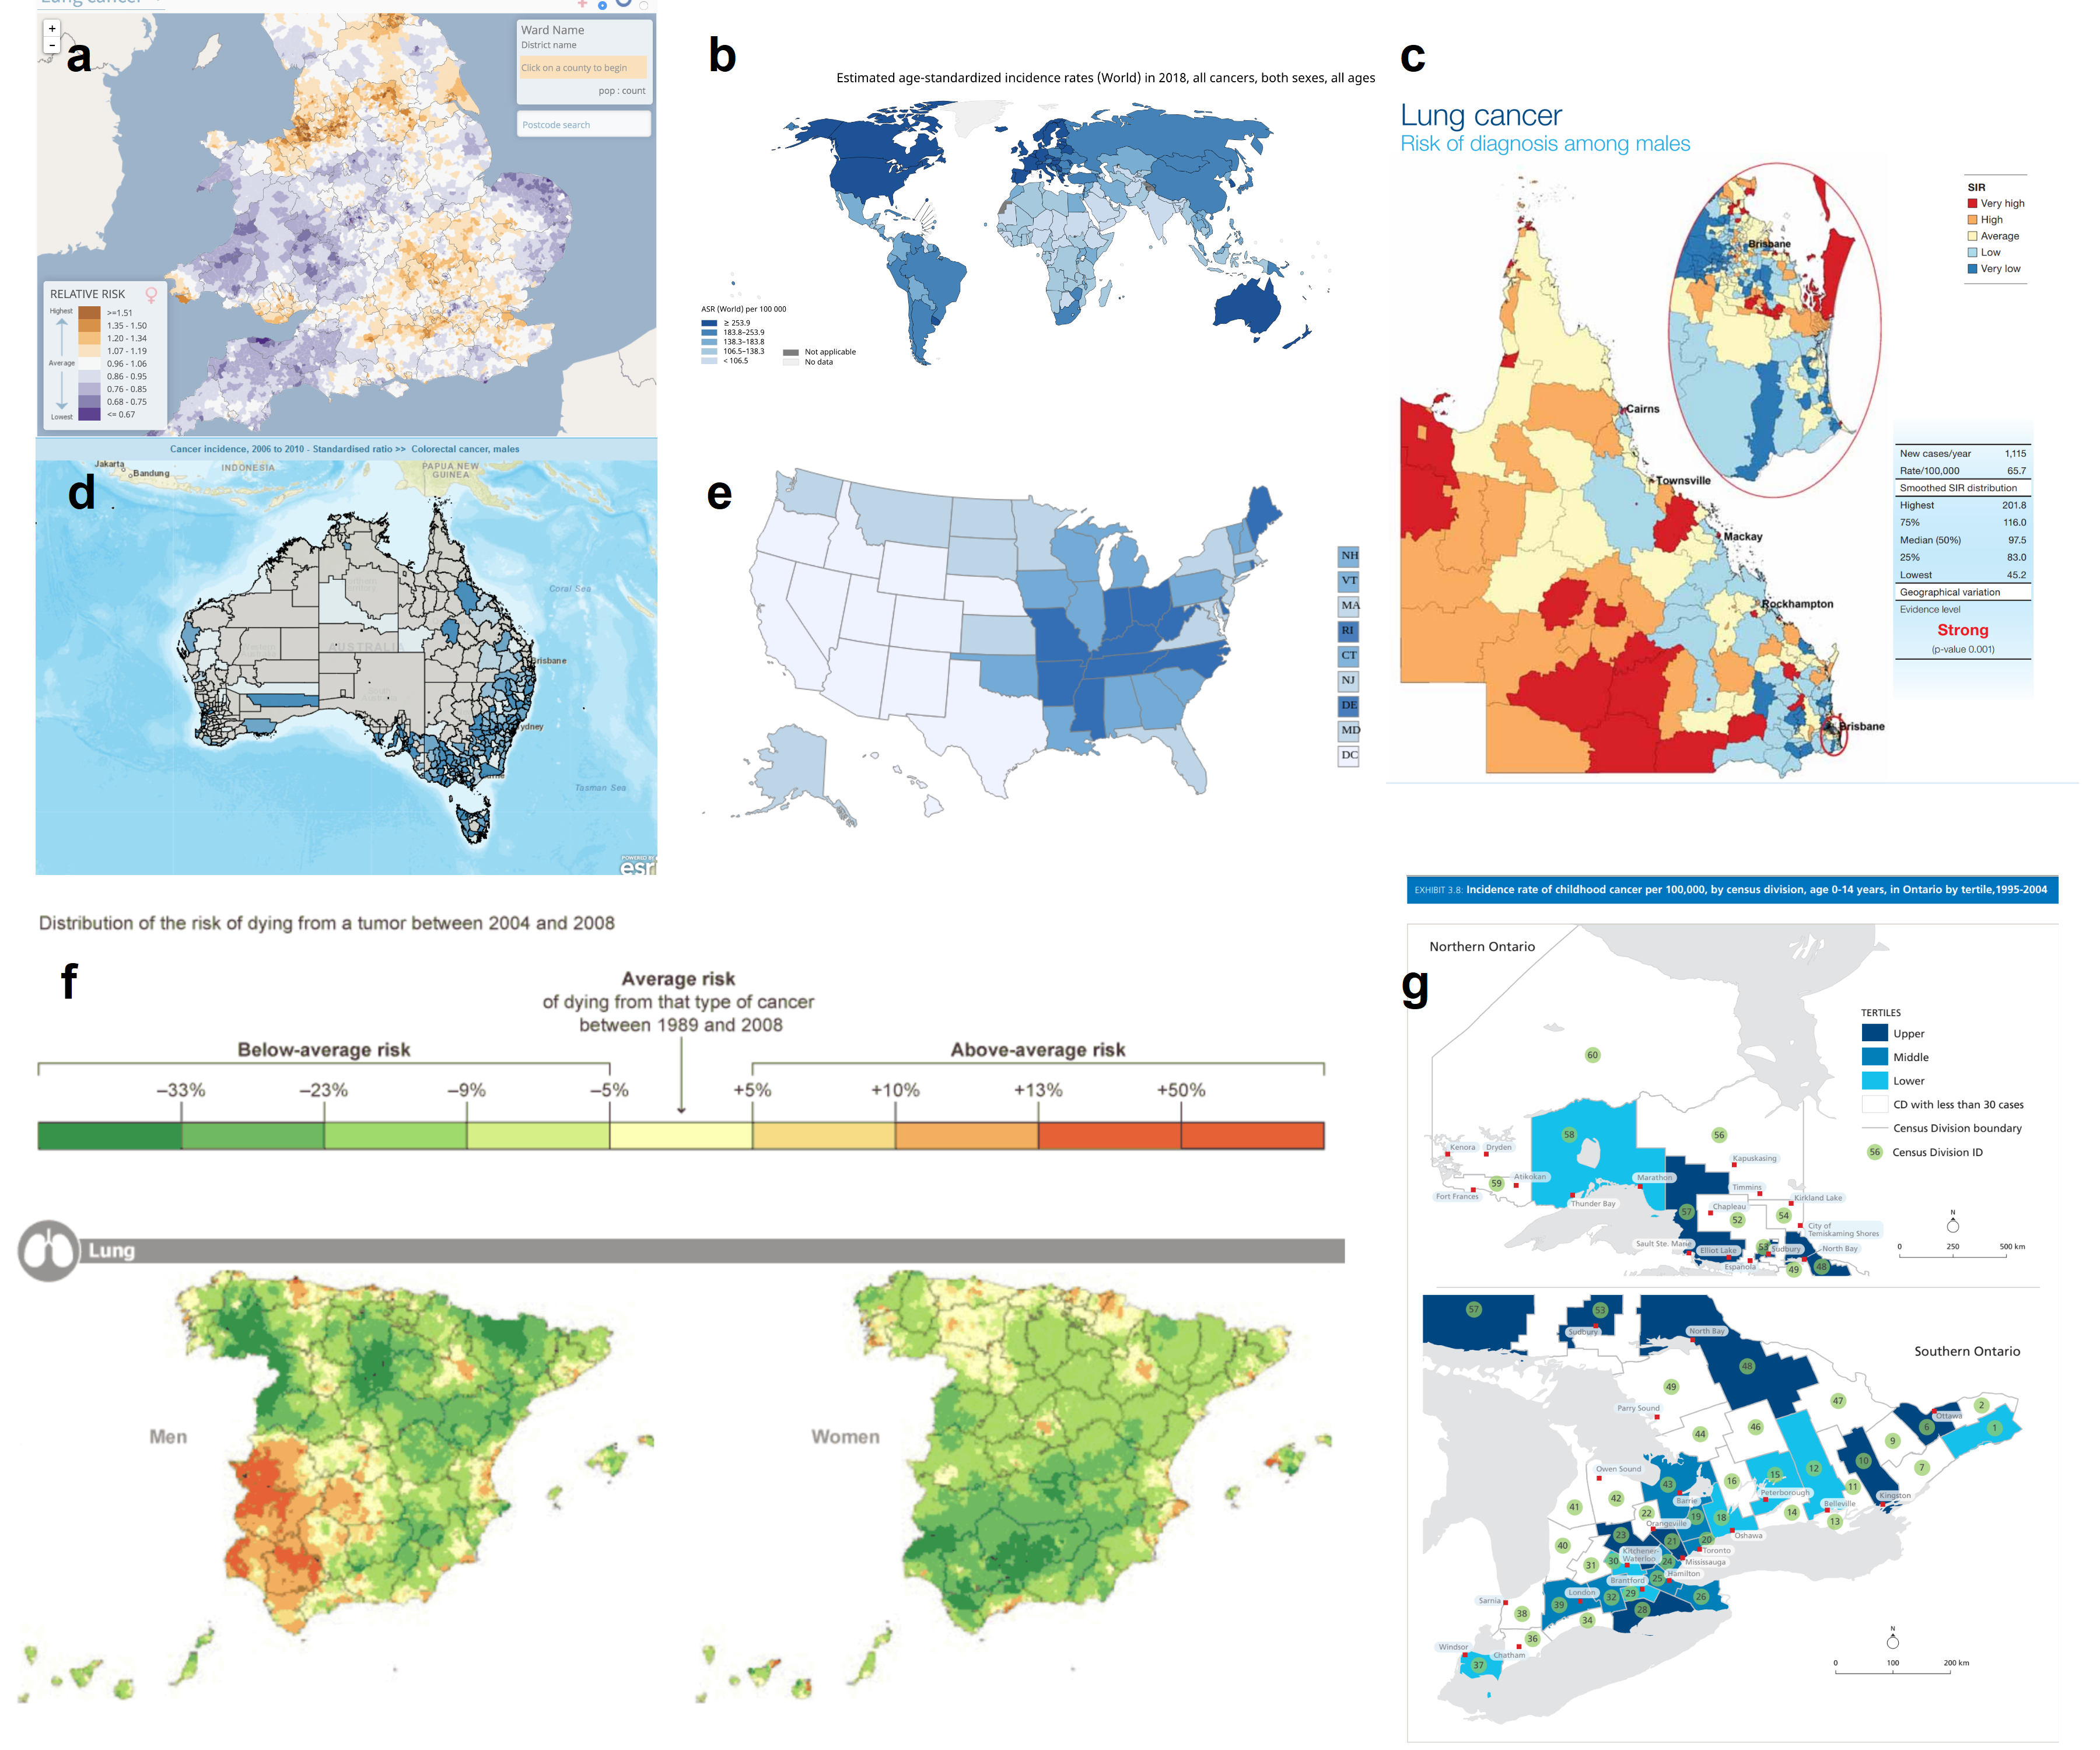
\includegraphics[width=50in]{figures/02-literature/choropleth_grid} 

}

\caption{ A selection of choropleth cancer maps from online atlases that are publicly available. Maps of various countries were chosen: United Kingdom, Australia, Spain, USA, Canada, and display several different colour palettes and legends. These atllases are described in Table 1.}\label{fig:choropleth-grid-create}
\end{figure}

\newpage

Table 1: A selection of choropleth cancer maps from online atlases.

\begin{longtable}[]{@{}clll@{}}
\toprule
\begin{minipage}[b]{0.08\columnwidth}\centering
Fig.\strut
\end{minipage} & \begin{minipage}[b]{0.20\columnwidth}\raggedright
Atlas\strut
\end{minipage} & \begin{minipage}[b]{0.35\columnwidth}\raggedright
Statistic\strut
\end{minipage} & \begin{minipage}[b]{0.26\columnwidth}\raggedright
Data source\strut
\end{minipage}\tabularnewline
\midrule
\endhead
\begin{minipage}[t]{0.08\columnwidth}\centering
1a\strut
\end{minipage} & \begin{minipage}[t]{0.20\columnwidth}\raggedright
The Environment and Health Atlas of England and Wales\strut
\end{minipage} & \begin{minipage}[t]{0.35\columnwidth}\raggedright
relative risk for women developing lung cancer in England and Wales in 2010 \autocite{EnvEnglandWales2}\strut
\end{minipage} & \begin{minipage}[t]{0.26\columnwidth}\raggedright
*\href{http://www.envhealthatlas.co.uk/homepage/}{Office for National Statistics (ONS) (England) and from the Welsh Cancer Intelligence and Surveillance Unit (WCISU)*}\strut
\end{minipage}\tabularnewline
\begin{minipage}[t]{0.08\columnwidth}\centering
1b\strut
\end{minipage} & \begin{minipage}[t]{0.20\columnwidth}\raggedright
Globocan 2018: Estimated Cancer Incidence, Mortality and Prevalence Worldwide\strut
\end{minipage} & \begin{minipage}[t]{0.35\columnwidth}\raggedright
age standardized incidence rates (per 100,000) for all invasive cancers for both men and women, aggregated at a national level for 2018 \autocite{Globocan}\strut
\end{minipage} & \begin{minipage}[t]{0.26\columnwidth}\raggedright
\emph{\href{https://www.iarc.fr/}{World Health Organization's International Agency for Research on Cancer}}.\strut
\end{minipage}\tabularnewline
\begin{minipage}[t]{0.08\columnwidth}\centering
1c\strut
\end{minipage} & \begin{minipage}[t]{0.20\columnwidth}\raggedright
Atlas of Cancer in Queensland\strut
\end{minipage} & \begin{minipage}[t]{0.35\columnwidth}\raggedright
the relative incidence ratio of lung cancer in males in the state of QLD within Australia based on data from 1998 to 2007, Queensland Cancer Council\autocite{QLDcancerAtlas}\strut
\end{minipage} & \begin{minipage}[t]{0.26\columnwidth}\raggedright
\emph{\href{https://cancerqld.org.au/research/cancer-registries/queensland-cancer-registry/}{Queensland Cancer Registry}}\strut
\end{minipage}\tabularnewline
\begin{minipage}[t]{0.08\columnwidth}\centering
1d\strut
\end{minipage} & \begin{minipage}[t]{0.20\columnwidth}\raggedright
Bowel Cancer Australia Atlas\strut
\end{minipage} & \begin{minipage}[t]{0.35\columnwidth}\raggedright
the percentage of Australian males between 50 - 54 years of age diagnosed with bowel cancer in 2016 in Australia \autocite{Bowel}.\strut
\end{minipage} & \begin{minipage}[t]{0.26\columnwidth}\raggedright
\emph{\href{https://www.bowelcanceraustralia.org/}{Bowel Cancer Australia}}\strut
\end{minipage}\tabularnewline
\begin{minipage}[t]{0.08\columnwidth}\centering
1e\strut
\end{minipage} & \begin{minipage}[t]{0.20\columnwidth}\raggedright
United States Cancer Statistics: An Interactive Cancer Statistics Website\strut
\end{minipage} & \begin{minipage}[t]{0.35\columnwidth}\raggedright
the incidence rate per 100,000, of all cancer types for men and women in the United States in 2016, aggregated at the state level \autocite{USInteractive}.\strut
\end{minipage} & \begin{minipage}[t]{0.26\columnwidth}\raggedright
\emph{\href{https://www.cdc.gov/}{Centers for Disease Control and Prevention}}, with data from state cancer registries.\strut
\end{minipage}\tabularnewline
\begin{minipage}[t]{0.08\columnwidth}\centering
1f\strut
\end{minipage} & \begin{minipage}[t]{0.20\columnwidth}\raggedright
Map of Cancer Mortality Rates in Spain\strut
\end{minipage} & \begin{minipage}[t]{0.35\columnwidth}\raggedright
side by side maps of relative risk of lung cancer for men vs women for 2004 to 2008 \autocite{cancerSpain}.\strut
\end{minipage} & \begin{minipage}[t]{0.26\columnwidth}\raggedright
\emph{\href{https://elpais.com/elpais/2014/10/06/media/1412612722_141933.html}{Map of cancer mortality rates in Spain}}\strut
\end{minipage}\tabularnewline
\begin{minipage}[t]{0.08\columnwidth}\centering
1g\strut
\end{minipage} & \begin{minipage}[t]{0.20\columnwidth}\raggedright
Atlas of Childhood Cancer in Ontario\strut
\end{minipage} & \begin{minipage}[t]{0.35\columnwidth}\raggedright
the incidence rate of childhood cancers per 100,000 (by census division) for children aged 0-14, in Ontario from 1995 to 2004 \autocite{OntarioPediatric}.\strut
\end{minipage} & \begin{minipage}[t]{0.26\columnwidth}\raggedright
\emph{\href{https://www.pogo.ca/research-data/pogonis-childhood-cancer-database/data-requests/}{The Pediatric Oncology Group of Ontario Networked Information System}}\strut
\end{minipage}\tabularnewline
\bottomrule
\end{longtable}

Epidemiologists and statisticians have developed the statistics used to communicate the burden of cancer over several decades. Table 2 summarizes the measures commonly presented in published cancer atlases. Mortality rates are commonly presented as relative rates of risk across the population and age-adjusted to correct for the higher prevalence of cancers in older populations. As described in Howe \autocite{HEDP}, Englishman P. Stocks advanced the field of mortality statistics by introducing the standardized mortality ratios in the 1930s, which is an improvement on crude death rates.

Table 2: Common measures for reporting cancer information.

\begin{longtable}[]{@{}ll@{}}
\toprule
\begin{minipage}[b]{0.28\columnwidth}\raggedright
Measure\strut
\end{minipage} & \begin{minipage}[b]{0.66\columnwidth}\raggedright
Details\strut
\end{minipage}\tabularnewline
\midrule
\endhead
\begin{minipage}[t]{0.28\columnwidth}\raggedright
1. Count\strut
\end{minipage} & \begin{minipage}[t]{0.66\columnwidth}\raggedright
Crude cancer counts\strut
\end{minipage}\tabularnewline
\begin{minipage}[t]{0.28\columnwidth}\raggedright
2. Rate per 100,000\strut
\end{minipage} & \begin{minipage}[t]{0.66\columnwidth}\raggedright
Cancer incidence per 100,000 population\strut
\end{minipage}\tabularnewline
\begin{minipage}[t]{0.28\columnwidth}\raggedright
3. IR (Incidence Ratio)\strut
\end{minipage} & \begin{minipage}[t]{0.66\columnwidth}\raggedright
\((IR)_i=\frac{(Incidence\ Rate)_i}{Average\ Incidence\ Rate}\),\strut
\end{minipage}\tabularnewline
\begin{minipage}[t]{0.28\columnwidth}\raggedright
\strut
\end{minipage} & \begin{minipage}[t]{0.66\columnwidth}\raggedright
The cancer incidence rate in region \(i\) over the average cancer incidence rate for all of the regions\strut
\end{minipage}\tabularnewline
\begin{minipage}[t]{0.28\columnwidth}\raggedright
4. Age-Adjusted Rate per 100,000\strut
\end{minipage} & \begin{minipage}[t]{0.66\columnwidth}\raggedright
Standardized by age structure or region\strut
\end{minipage}\tabularnewline
\begin{minipage}[t]{0.28\columnwidth}\raggedright
5. Age-Adjusted Relative Risk\strut
\end{minipage} & \begin{minipage}[t]{0.66\columnwidth}\raggedright
Standardized by age structure in each region \(i\)\strut
\end{minipage}\tabularnewline
\begin{minipage}[t]{0.28\columnwidth}\raggedright
6. SIR (Standardized Incidence Ratio)\strut
\end{minipage} & \begin{minipage}[t]{0.66\columnwidth}\raggedright
Incidence standardized by population at risk in each region \(i\)\strut
\end{minipage}\tabularnewline
\begin{minipage}[t]{0.28\columnwidth}\raggedright
7. Below or above Expected\strut
\end{minipage} & \begin{minipage}[t]{0.66\columnwidth}\raggedright
An alternative expression of the SIR\strut
\end{minipage}\tabularnewline
\begin{minipage}[t]{0.28\columnwidth}\raggedright
8. RER\strut
\end{minipage} & \begin{minipage}[t]{0.66\columnwidth}\raggedright
\(RER = \frac{(Cancer\ related\ mortality)_i}{Average\ cancer\ related\ mortality}\)\strut
\end{minipage}\tabularnewline
\begin{minipage}[t]{0.28\columnwidth}\raggedright
(Relative Excess Risk)\strut
\end{minipage} & \begin{minipage}[t]{0.66\columnwidth}\raggedright
Represents the estimate of cancer-related mortality within five years of diagnosis. Also referred to as `excess hazard ratio'\strut
\end{minipage}\tabularnewline
\bottomrule
\end{longtable}

Roberts \autocite{roberts2019communication} identified 33 cancer atlases published between 2010 and 2018. Each of these online atlases uses choropleth maps. All except one of these were published by non-commercial organizations, including not-for-profits, government, research organizations, advocacy groups or government-funded partnerships. Figure 1 displays a subset of maps from these atlases, the selection varies in the geographies explored. Figure 1b shows Globocan 2018 \autocite{Globocan} which explores Estimated Cancer Incidence, Mortality and Prevalence Worldwide using data sourced from cancer registries of each country. The Bowel Cancer Australia Atlas in Figure 1d presents an example of a cancer specific atlas -- it shows the average Standardized Incidence Ratio of colorectal cancer for Australian males from 2006 to 2010 \autocite{Bowel}. Like many of the atlases examined, there is a choice of gender displayed in the Bowel Cancer Atlas. Gender is displayed in side-by-side maps in the Map of Cancer Mortality Rates in Spain (Figure 1f) \autocite{cancerSpain}.

Resolution of the maps varies greatly. Figure 1b shows global information at a national level. The United States Cancer Statistics \autocite{USInteractive} shows data aggregated at the state level. The Environment and Health Atlas of England and Wales \autocite{EnvEnglandWales2} (Figure 1a) shows the relative risk for women developing lung cancer at a neighborhood (small-area) scale. The Atlas of Cancer in Queensland (Figure 1c) shows the relative incidence ratio of lung cancer in males for each Statistical Area at Level 2 \autocite{abs2016} in the state of Queensland within Australia \autocite{QLDcancerAtlas}.

Age-specific atlases are less common. Figure 1g displays Atlas of Childhood Cancer in Ontario, this communicates the incidence rate of childhood cancers per 100,000 (by census division) for children aged 0-14, in Ontario from 1995 to 2004 \autocite{OntarioPediatric}.

\hypertarget{additional-considerations}{%
\subsection{Additional considerations}\label{additional-considerations}}

Cancer atlases often display supplementary graphs and plots to add more information. Additional materials such as tables, graphs, and text explanations support understanding and inference derived from maps, ensuring the message communicated will be consistent across a range of viewers \autocite{CPISACA}. The many displays of statistical summaries, including dot plots, bar plots, box plots, cumulative distribution plots, scatter plots, and normal probability plots, can provide alternative views of the cancer statistics. These can also display supporting statistics such as error, confidence intervals, distributions, sample or population sizes, and standard deviation.

The statistics communicated in atlases are often used to describe differences between areas. This can occur at different levels of aggregation. Aggregation of global health statistics occurs within administrative and arbitrarily defined regions, such as those used by the World Health Organization and the United Nations \autocite{IARC_3}. World atlases can allow for displays of data aggregated into continents, countries, states, provinces and congressional districts \autocite{USInteractive}. Each population area will probably have a different number of people, which is typically used to calibrate the statistic. Cancer atlases may also communicate the distribution of the population living in all areas in a table or histogram display \autocite{NICR_1}. Atlases can connect the population to the land available to them by communicating population density.

Maps can also be used to focus on demographic strata, such as age and sex. Some of the digital atlases surveyed allow subsets such as males, females, or those aged over 65, to be selected for display. Similarly, socioeconomic indicators, such as unemployment rates, poverty rates, remoteness, and education levels, can be used to filter data, in order to communicate how cancer prevalence varies for different members of society. Few atlases provide this level of detail.

Introducing population and demographic information helps to interpret the rates in areas effectively, but there will still be uncertainty around the rates. To address this, a cancer atlas often communicates uncertainty about the value of a statistic. There are several potential sources of uncertainty: sampling error, errors arising from the disease reporting process (or data collection), and errors arising from the statistical modelling or simulation process. The most common measures used to present uncertainty are credible or confidence intervals (CIs). Displaying the uncertainty associated with reported statistics is a vital feature of a cancer map, but it is difficult to display effectively. The map focuses on displaying the statistic and lacks additional space to represent the uncertainty. Providing an adjacent map or overlaying maps with symbols \autocite{VSSDCUC} are two common solutions.

\hypertarget{ch:chorolimit}{%
\subsection{Limitations of choropleth displays}\label{ch:chorolimit}}

Australia presents an extreme case of an urban rural divide. The land mass occupied by urban electoral districts is only 10\% of Australia, yet 90\% of the population live in these urban areas \autocite{ACTUC}.

Choropleth maps provide a familiar display, which shows data in a geographically recognisable way. A disadvantage is that the different population and geographical sizes of administrative areas can attract attention to the shades of the underpopulated but large areas \autocite{EI}. Skowronnek also \autocite{BCM} discusses how choropleth maps suffer from area-size bias, as they give a `stronger visual weight' to large administrative units. The administrative boundaries used to define regions may limit a choropleth display, as this display unfaithfully represents the disease distribution across the region by obscuring small geographic areas. Sparsely populated rural areas are emphasized, whereas the areas representing inner city communities are very small. This is especially true for Australia.

Choropleth maps colour each geographic unit to allow map users to measure the value of the statistic \autocite{EI}. Map users contrast the colours in neighbouring areas to understand the spatial distribution. The ColorBrewer system \autocite{CB} and viridis \autocite{viridis} palettes provide effective colour schemes for qualitative, sequential and diverging data. When communicating information using colour, a map creator should use a scheme that has a linear color gradient, with perceptually uniform color spaces that match equal steps in data space with equal steps in the colour space \autocite{PUCS}.
The use of borders and backgrounds, and their colours, can also change the appearance of the colors representing the value of the statistics \autocite{CB}. These supports can be used to implement a reference point in the colour scheme as well as orient users to the geographic regions.

Inset maps like in Brisbane city in Figure 1c of the state of Queensland are commonly used to reduce distorted interpretations, but it is a bandaid remedy. For Australia, many, many inset maps would be needed.

\hypertarget{ch:alternatives}{%
\section{Contemporary alternatives to choropleth maps}\label{ch:alternatives}}

\hypertarget{cartograms}{%
\subsection{Cartograms}\label{cartograms}}

Choropleth maps imply uniformity of data across the geographic space but population densities are unlikely to be uniform \autocite{BCM}. Cartographers developed the cartogram to draw the attention to the population by transforming the map \autocite{ACCAC}. The resulting display can communicate the impact of the disease more accurately across the population, as recorded by the statistic, at the sacrifice of geographic accuracy.

When a map creator desires a uniform population density of the map base, the purposeful distortion of the map space is beneficial. The ``population distribution is often extremely uneven'', making a distortion necessary so that population is more faithfully represented as a uniformly distributed background for the statistic to be presented \autocite{ACTUC} \autocite{CTTMB} \autocite{GOINO}. An area cartogram \autocite{NAC}, or population-by-area cartogram \autocite{TAAM} is produced from the distortion of the geographical shape according to population. Event cartograms \autocite{VSSDCUC} change the area of regions on a map depending on the amount of disease-related events, rather than population.

Cartograms provide an alternative visualization method for statistical and geographical information. Monmonier \autocite{HTLWM} suggests that map creators can use white lies to create useful spatial displays. It is easy for the reader to disregard the impact of transformations used to create cartograms, for the benefit of reading the statistical distribution more accurately with approximate geographic information. The spatial transformation of map regions relative to the data emphasizes the data distribution instead of land size \autocite{CBATCC}. When visualizing population statistics, Dorling considers this design `more socially just' \autocite{ACTUC}, or honest \autocite{NISCC}, giving equitable representation and attention to all members of the population and reducing the visual impact of large areas with small populations \autocite{DMAHP}. Howe \autocite{HEDP} suggests that `cancer occurs in people, not in geographical areas' and that spatial socio-economic data, like cancer rates, are best presented on a cartogram for urban areas as the population map base avoids allocating `undue prominence' to rural areas \autocite{CTTMB}.

The creation of cartograms was historically in the hands of professional cartographers \autocite{CD}. Early approaches by John Hunter and Jonathan Young (1968) and Durham's wooden tile method, Skoda and Robertson's (1972) steel ball-bearing approach and Tobler's (1973) computer programs \autocite{ACTUC}. Howe \autocite{HEDP} discusses the impact of electronic computer-assisted techniques. Geographical information systems allow map creators to produce cartograms and they use these systems depending on `the effectiveness, efficiency, and satisfaction of the map products' \autocite{CD}.

There are two key issues to consider when creating alternative map displays, (1) the intended audience of the map, and (2) its purpose. Nusrat and Kobourov \autocite{SAIC} provided a framework to investigate implementations of the many algorithms presented, and the ``statistical accuracy, geographical accuracy, and topological accuracy''.

\begin{Shaded}
\begin{Highlighting}[]
\NormalTok{knitr}\OperatorTok{::}\KeywordTok{include_graphics}\NormalTok{(}\StringTok{"figures/02-literature/usa_grid.png"}\NormalTok{)}
\end{Highlighting}
\end{Shaded}

\begin{figure}
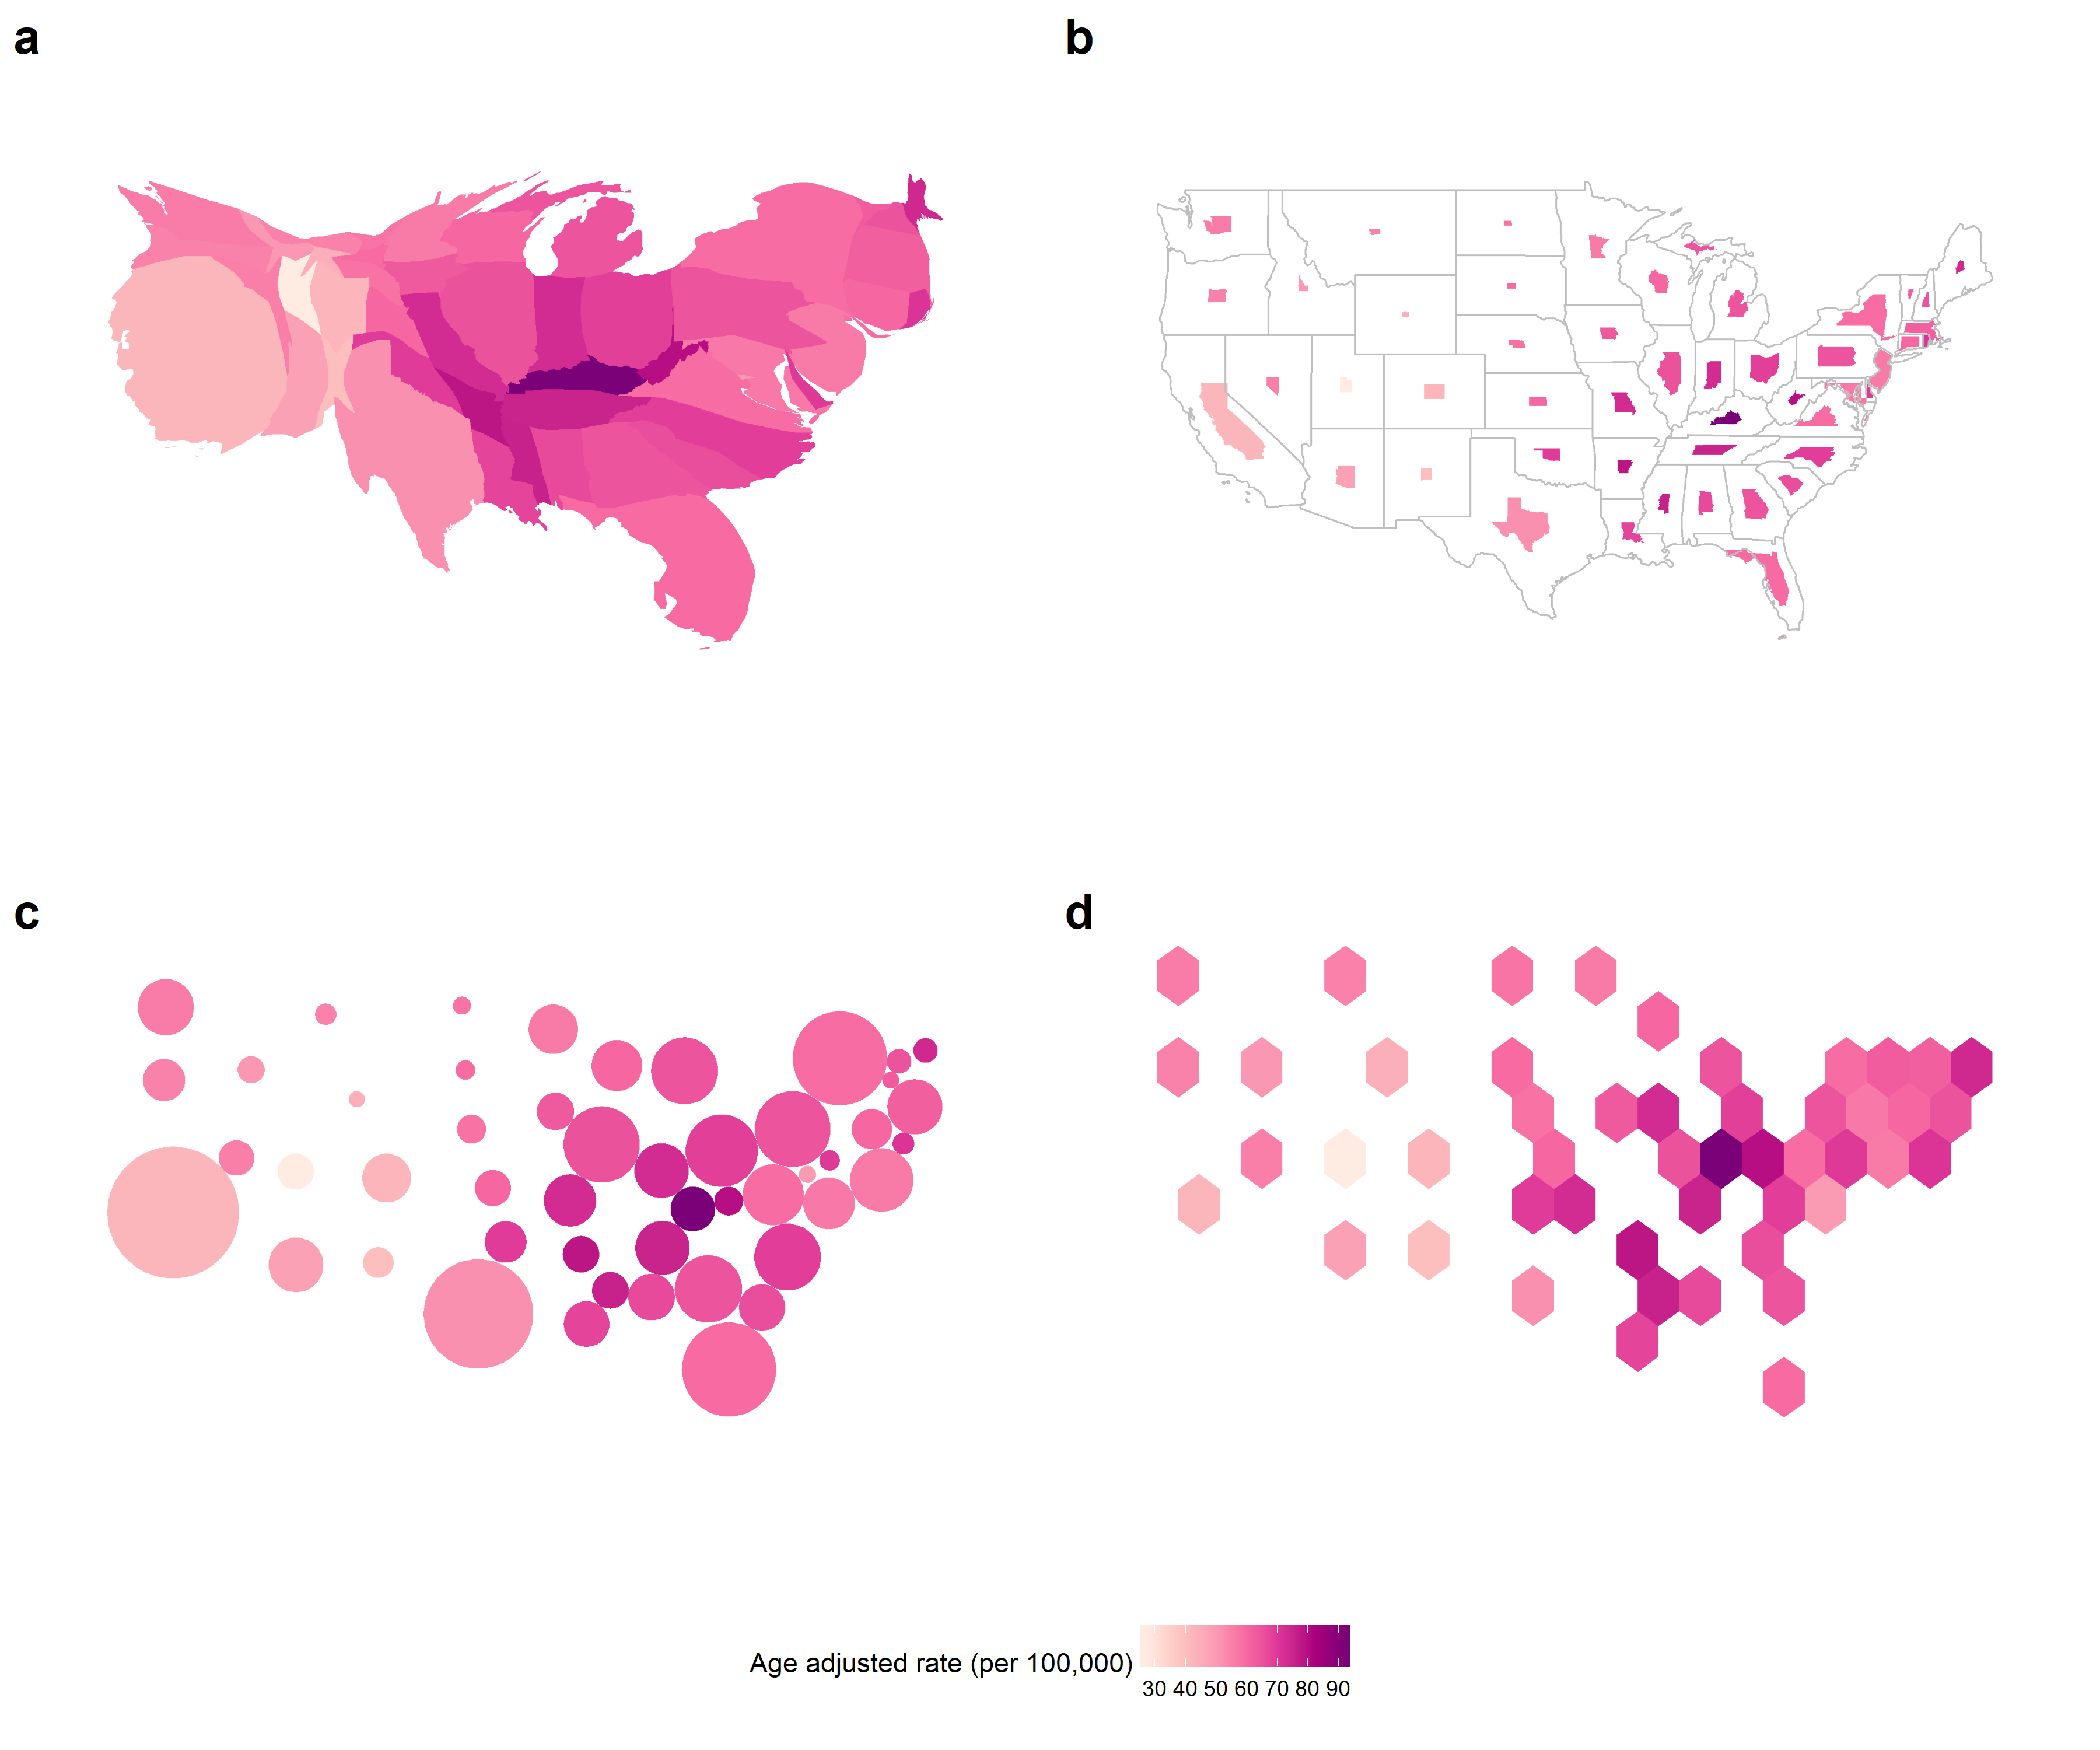
\includegraphics[width=50in]{figures/02-literature/usa_grid} \caption{ Common alternatives to maps, showing the same information for the United States of America: (a) contiguous cartogram, (b) non-contiguous, shape-preserved cartogram, (c)  Dorling cartogram (non-contiguous), (d) hexagon tilemap (non-contiguous). Maps (a) - (c) are created by resizing and reshaping the states of the USA to match the 2015 population of the state. This provides a better sense of the extent of disease relative to the population in the country and can help ease losing information about physically small but population-dense states. Map creators give each state equal size and thus equal emphasis in (d) the hexagon tile map.}\label{fig:ggcartograms}
\end{figure}

Table 3: Maps used to present statistics for the United States of America. The colour of each state communicates the average age-adjusted rate of incidence for lung and bronchus for females and males in the United States 2012-2016.

\begin{longtable}[]{@{}ll@{}}
\toprule
\begin{minipage}[b]{0.28\columnwidth}\raggedright
Map display\strut
\end{minipage} & \begin{minipage}[b]{0.66\columnwidth}\raggedright
Details\strut
\end{minipage}\tabularnewline
\midrule
\endhead
\begin{minipage}[t]{0.28\columnwidth}\raggedright
a. Contiguous\strut
\end{minipage} & \begin{minipage}[t]{0.66\columnwidth}\raggedright
It has distorted each state's shape according to the population of the state in 2015. The state of California has become much larger because of the large population density. This draws attention to the densely populated North-East region and detracts from the less populated Mid West.\strut
\end{minipage}\tabularnewline
\begin{minipage}[t]{0.28\columnwidth}\raggedright
b. Non-contiguous\strut
\end{minipage} & \begin{minipage}[t]{0.66\columnwidth}\raggedright
It maintains the geographic shape of the states, but the size has altered according to the population of the state in 2015. The state of California has remained closer to its original size than its surrounding states. The North-East states have remained closer to their geographical size, for Massachusetts and Connecticut. This draws attention to the densely populated North-East region and the sparse Mid West.\strut
\end{minipage}\tabularnewline
\begin{minipage}[t]{0.28\columnwidth}\raggedright
c.~Dorling\strut
\end{minipage} & \begin{minipage}[t]{0.66\columnwidth}\raggedright
Circles are used to represent each state, but the population of the state determines the size in 2015. The North-East states remain closer to their neighbors and are slightly displaced from their geographic location. It highlights the sparsity of the population in the Mid West by the distance between the circles at the geographic centroids.\strut
\end{minipage}\tabularnewline
\begin{minipage}[t]{0.28\columnwidth}\raggedright
d.~Hexagon Tessellation\strut
\end{minipage} & \begin{minipage}[t]{0.66\columnwidth}\raggedright
A hexagon of equal size represents each state. It is easy to contrast the neighboring states however the North-East regions have been displaced from their geographic location. It highlights the sparsity of the population in the Mid West by the light yellow color, the Age-Adjusted rate in Kentucky is the darkest and its neighbors are similar.\strut
\end{minipage}\tabularnewline
\bottomrule
\end{longtable}

Figure 2 shows four different cartograms for the same data. The information in Table 3 summarizes what can be observed in the four types of cartograms.

\hypertarget{contiguous}{%
\subsubsection{Contiguous}\label{contiguous}}

A contiguous cartogram alters the choropleth according to a statistic and maintains connectivity of the map regions. Min Ouyang and Revesz \autocite{ACA} present three algorithms for creating value-by-area cartograms. They implement `map deformation' to account for the value assigned to each area. Other methods include Tobler's Pseudo-Cartogram Method, Dorling's Cellular Automaton Method \autocite{ACTUC}, Radial Expansion Method, Rubber Sheet Method, Line Integral Method, Constraint-Based Method \autocite{CBATCC}.

Figure 2a shows a population contiguous cartogram of the United States. All states are visible and the shape of the United States overall is still recognizable. In contrast, Figure 3 a shows an Australian contiguous cartogram also based on population. The south east is enlarged, but high population areas are still small, and low population areas are still large on the map. The algorithm doesn't fully reach an optimal configuration where area matches population -- Australia is too heterogeneous for the algorithm to handle.

To be able to recognize the significant changes, a reader will usually have to know the initial geography to find the differences in the new cartogram layout \autocite{NAC}. The shapes of small areas on a choropleth map and a cartogram are preserved using Tobler's Conformal mapping method.
Koccmoud and House \autocite{CBATCC} present this issue as conflicting tasks or aims, to adjust region sizes and retain region shapes.

\hypertarget{non-contiguous}{%
\subsubsection{Non-contiguous}\label{non-contiguous}}

Non-contiguous cartograms prioritize the shapes of the areas instead of connectivity. Each area stays in a similar position to its location on a choropleth map. Displaying the choropleth map base allows map users to make comparisons regarding the change in the area. The addition is the gap between areas, created as each area shrinks or grows according to the associated value of the statistic. Olson \autocite{NAC} discusses the creation of these maps and the significance of the empty areas left between the geographic boundaries and the new shape.

The white space presents the meaningful empty-space property \autocite{ECGC}, \autocite{NAC} but it also distracts the reader from the data, with a low data density \autocite{TVDQI}.

\hypertarget{dorling}{%
\subsubsection{Dorling}\label{dorling}}

Daniel Dorling presents an alternative display engineered to highlight the spatial distribution and neighborhood relationships without complex distortions of borders and boundaries \autocite{ACTUC}:

\begin{quote}
``If, for instance, it is desirable that areas on a map have boundaries which are as simple as possible, why not draw the areas as simple shapes in the first place?''
\end{quote}

He acknowledged the sophistication of contiguous cartograms but critiqued their `very complex shapes,' he answers this with his implementation of maps created using `the simplest of all shapes'. Circular cartograms use the same circle shape for every region represented, resized according to the statistic represented or the population. This simple shape may be more effective for understanding the spatial distribution than contiguous cartograms. Contiguous cartograms create `nonsense' shapes that have `no meaning' \autocite{NISCC}. Both methods applies a gravity model to produce a layout, that avoids overlaps and keep spatial relationships with neighboring areas over many iterations. The circular cartogram is relatively fast to compute.

Raisz \autocite{RSCW} laid the groundwork for this approach in the mid-1930s, drawing rectangular cartograms that provide simple comparisons, effective for correcting misconceptions communicated by geographic maps. Tobler \autocite{TFYCC} names and defines these as Value-Area Cartograms. This rectangular display may sacrifice contiguity but allows for tiling where geographic neighbors placed in suitable relative positions also share borders \autocite{CDWCS}. Rectangular cartograms communicate bivariate displays of the population by the size of each rectangular, and they use color to communicate a second variable \autocite{ORC}.

\hypertarget{tile-map}{%
\subsection{Tile Map}\label{tile-map}}

A tile map provides a tessellated display of consistent shapes. A similar method to a rectangular cartogram, represents each geographic area using a square. The squares are tessellated to create a grid. Each area is represented by a square of the same dimensions, each tile is usually one unit of measurement, this could be geographic regions such as states or population-based that use a consistent measure of population for each tile. Regions with over four neighbors require some necessary displacement. The tile map uses color to represent a value of a statistic for each area. A similar method to a rectangular cartogram represents each geographic area using a square of the same dimensions. There are online media sources using this method, these include \autocite{NPR}, \autocite{FiveThirtyEight}, \autocite{WSJ}, \autocite{WP}. Tile maps may be difficult to create as they are best created manually, they require additional time and care as the number of geographic areas to include increases.

Cano and others \autocite{MDAC} define the term `mosaic cartograms' for hexagonal tile displays, where the number of tiles for each area or the color of them can communicate the statistic of regions. When using several tiles per region, map makers can adjust the complexity of the boundaries in the resulting display. They can also make a trade-off between boundary complexity and simplicity by the size of the tiles used.

\hypertarget{geofacet}{%
\subsection{Geofacet}\label{geofacet}}

Hafen \autocite{IGF} introduces the term geofacet to describe a grid display of small plots. The arrangement of tiles mimics the geographic topology. Geofaceting has the functionality that a statistical plot can be constructed in each facet for each geographic area. A tile map can communicate only one value per region in a visualization, while geofaceting is a more flexible visualization for communication as it increases the amount of information displayed. Virtually any type of plot can be shown in the tile, allowing displays of multiple variables or values per geographic entity. Creating the layout of a geofacet is manual, but once created can be used for any data on that geographic base.

\begin{Shaded}
\begin{Highlighting}[]
\NormalTok{knitr}\OperatorTok{::}\KeywordTok{include_graphics}\NormalTok{(}\StringTok{"figures/02-literature/gggrids.png"}\NormalTok{)}
\end{Highlighting}
\end{Shaded}

\begin{figure}
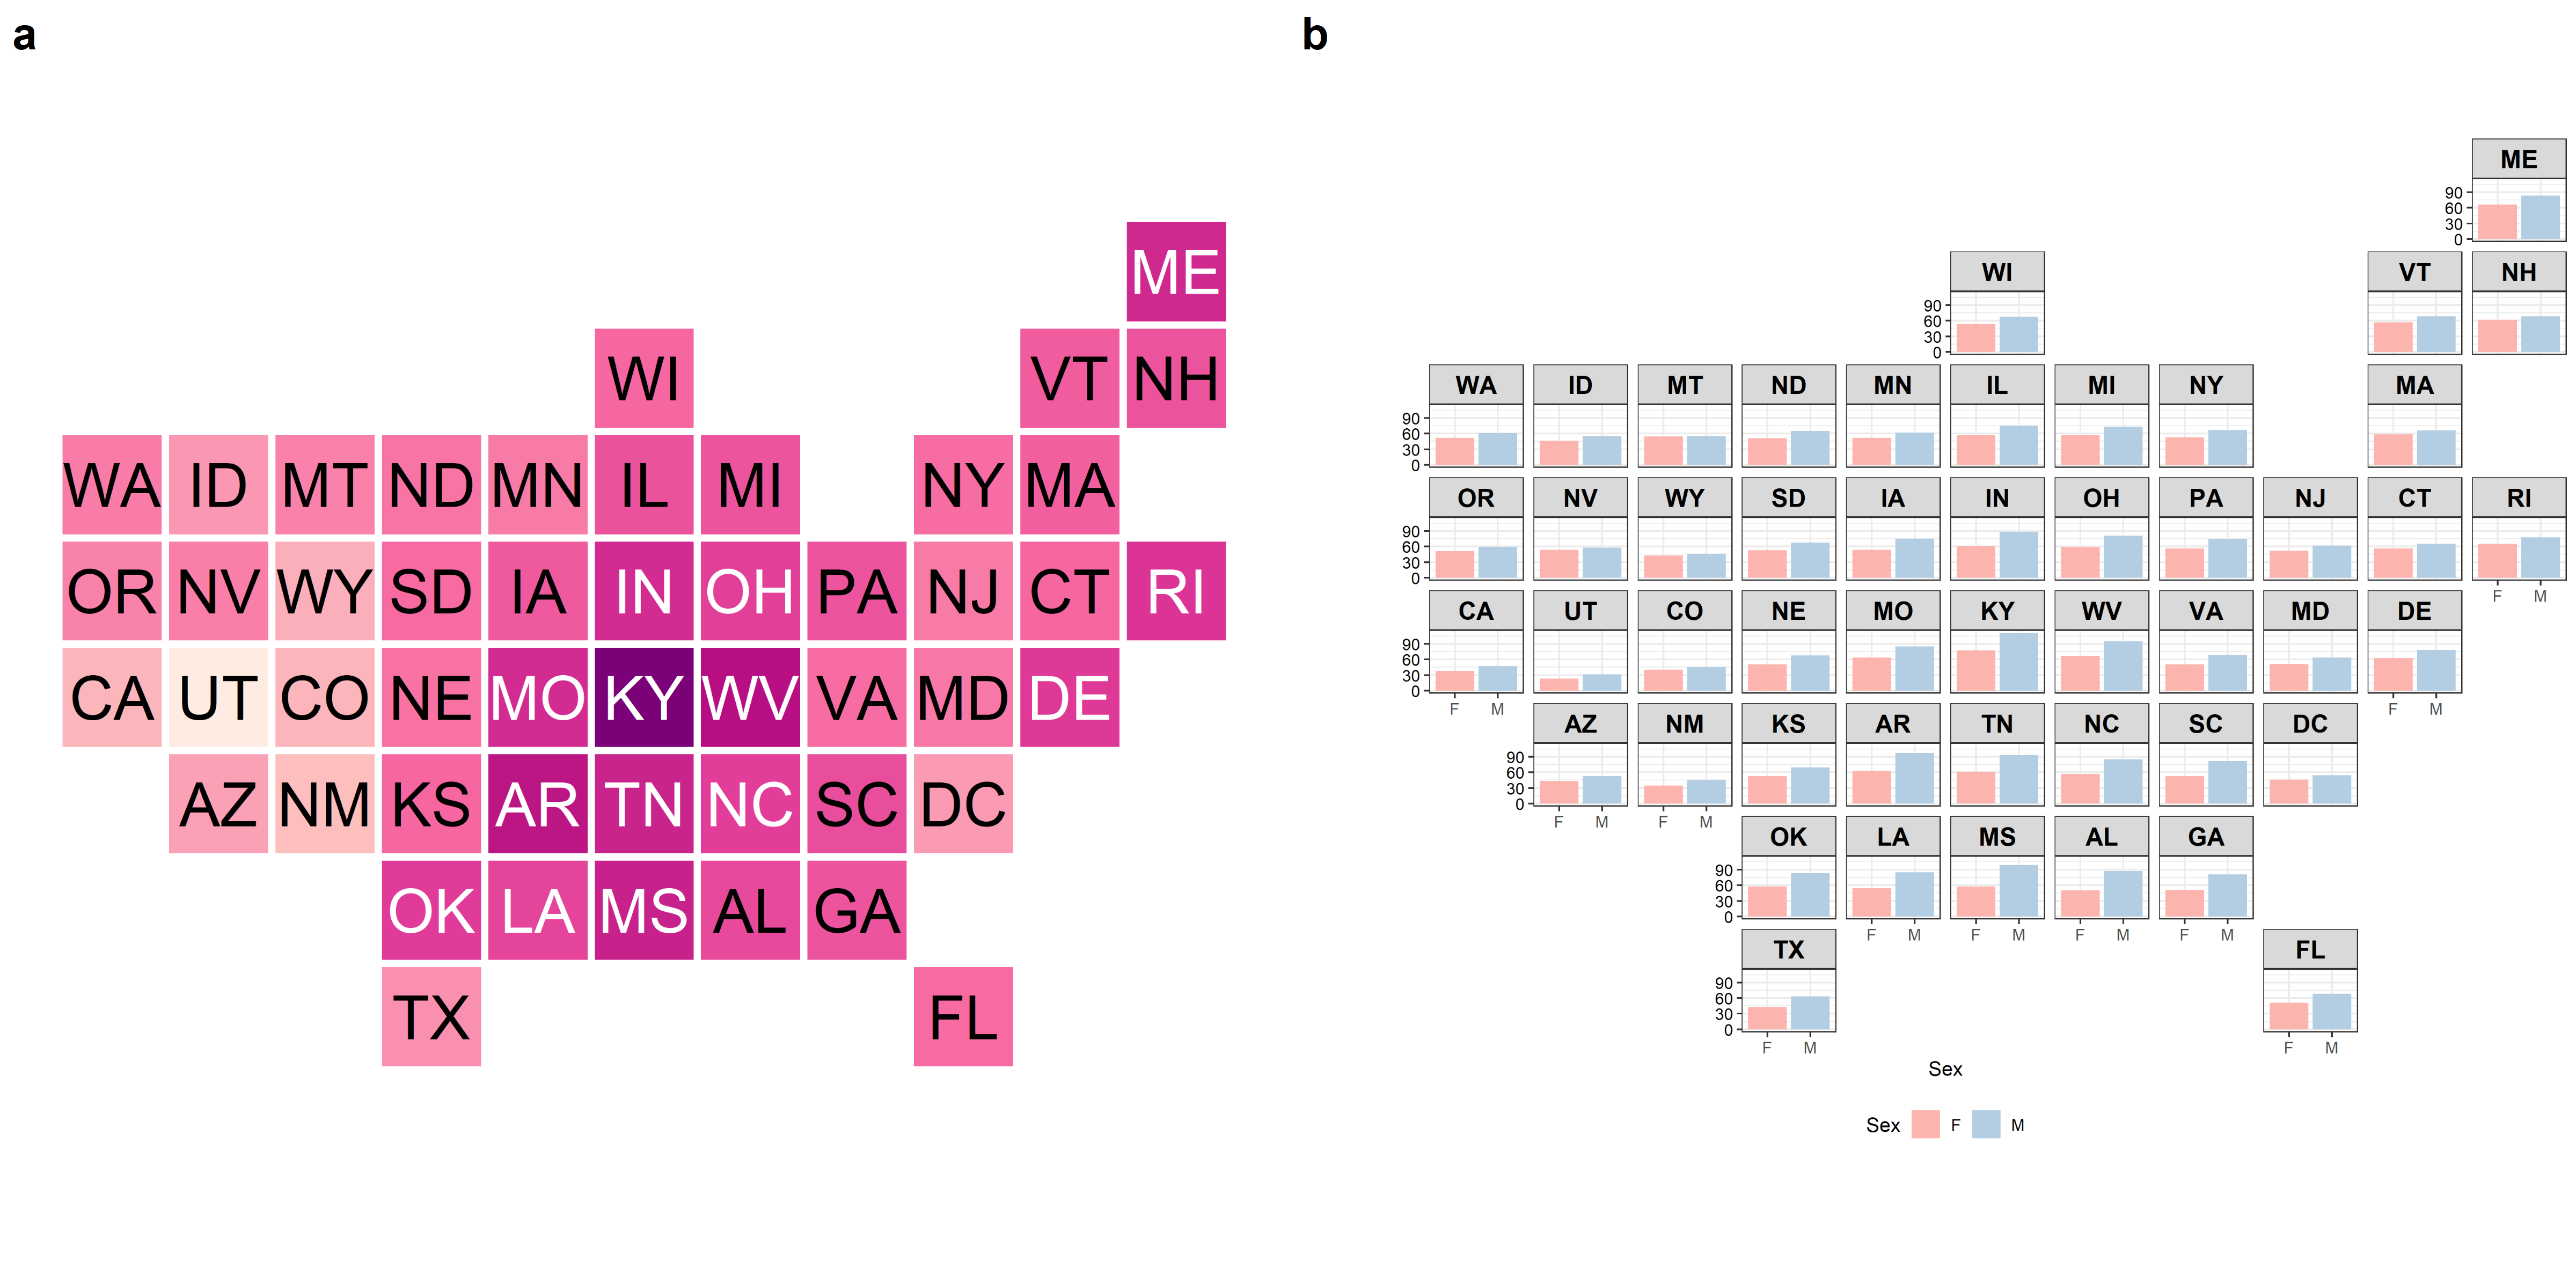
\includegraphics[width=1\linewidth]{figures/02-literature/gggrids} \caption{ Two alternative displays, tile map (left) and geofaceted map (right), showing state age-adjusted rate of incidence for lung and bronchus in the USA. In the tile map, the layout approximates spatial location, with each state being an equal box filled with color representing cancer incidence. The geo-faceted map shows bar charts laid out in a grid approximating the spatial location of the state. The maps show age-adjusted rates for males and females. This display allows the presentation of multiple variables for each geographic area.}\label{fig:ggtilemap}
\end{figure}

\hypertarget{multivariate-displays}{%
\subsection{Multivariate displays}\label{multivariate-displays}}

Pickle and others \autocite{MMST} present linked micromap plots to match geographic and statistical data visually, this serves as a solution to multi-dimensionality issues. These maps group areas based on their value for one variable, and additional columns provide displays that contrast the areas in each group by other variables. The display juxtaposes choropleth maps and statistical plots; it shows one map per group of the key separating variable, in a row with each additional statistical plot. Linked micromaps predominantly use the choropleth map for displays of spatial relationships. These maps show spatial relationships by allotting spatial neighbors to the same group. It is one of several alternative displays that allow maps to become bivariate displays, commonly used to present both an estimate and the associated uncertainty.

Lucchesi and Wikle \autocite{VUADBC} present bivariate choropleth maps blend color schemes to convey the intersection of categorized levels of an estimate and the associated uncertainty for each spatial area. They also suggest map pixilation, which breaks each region into small pixels, and allocates values to the individual pixels to create texture. This reflects the uncertainty around the area's estimate by randomly sampling from the confidence interval of the estimate of the area. Animating these displays involves resampling the pixels for each frame. Areas with uncertain values will flicker more dramatically than areas with more certain values.

\hypertarget{comparison-and-critique-of-alternative-displays}{%
\section{Comparison and critique of alternative displays}\label{comparison-and-critique-of-alternative-displays}}

\begin{Shaded}
\begin{Highlighting}[]
\NormalTok{knitr}\OperatorTok{::}\KeywordTok{include_graphics}\NormalTok{(}\StringTok{"figures/02-literature/auscartograms.png"}\NormalTok{)}
\end{Highlighting}
\end{Shaded}

\begin{figure}
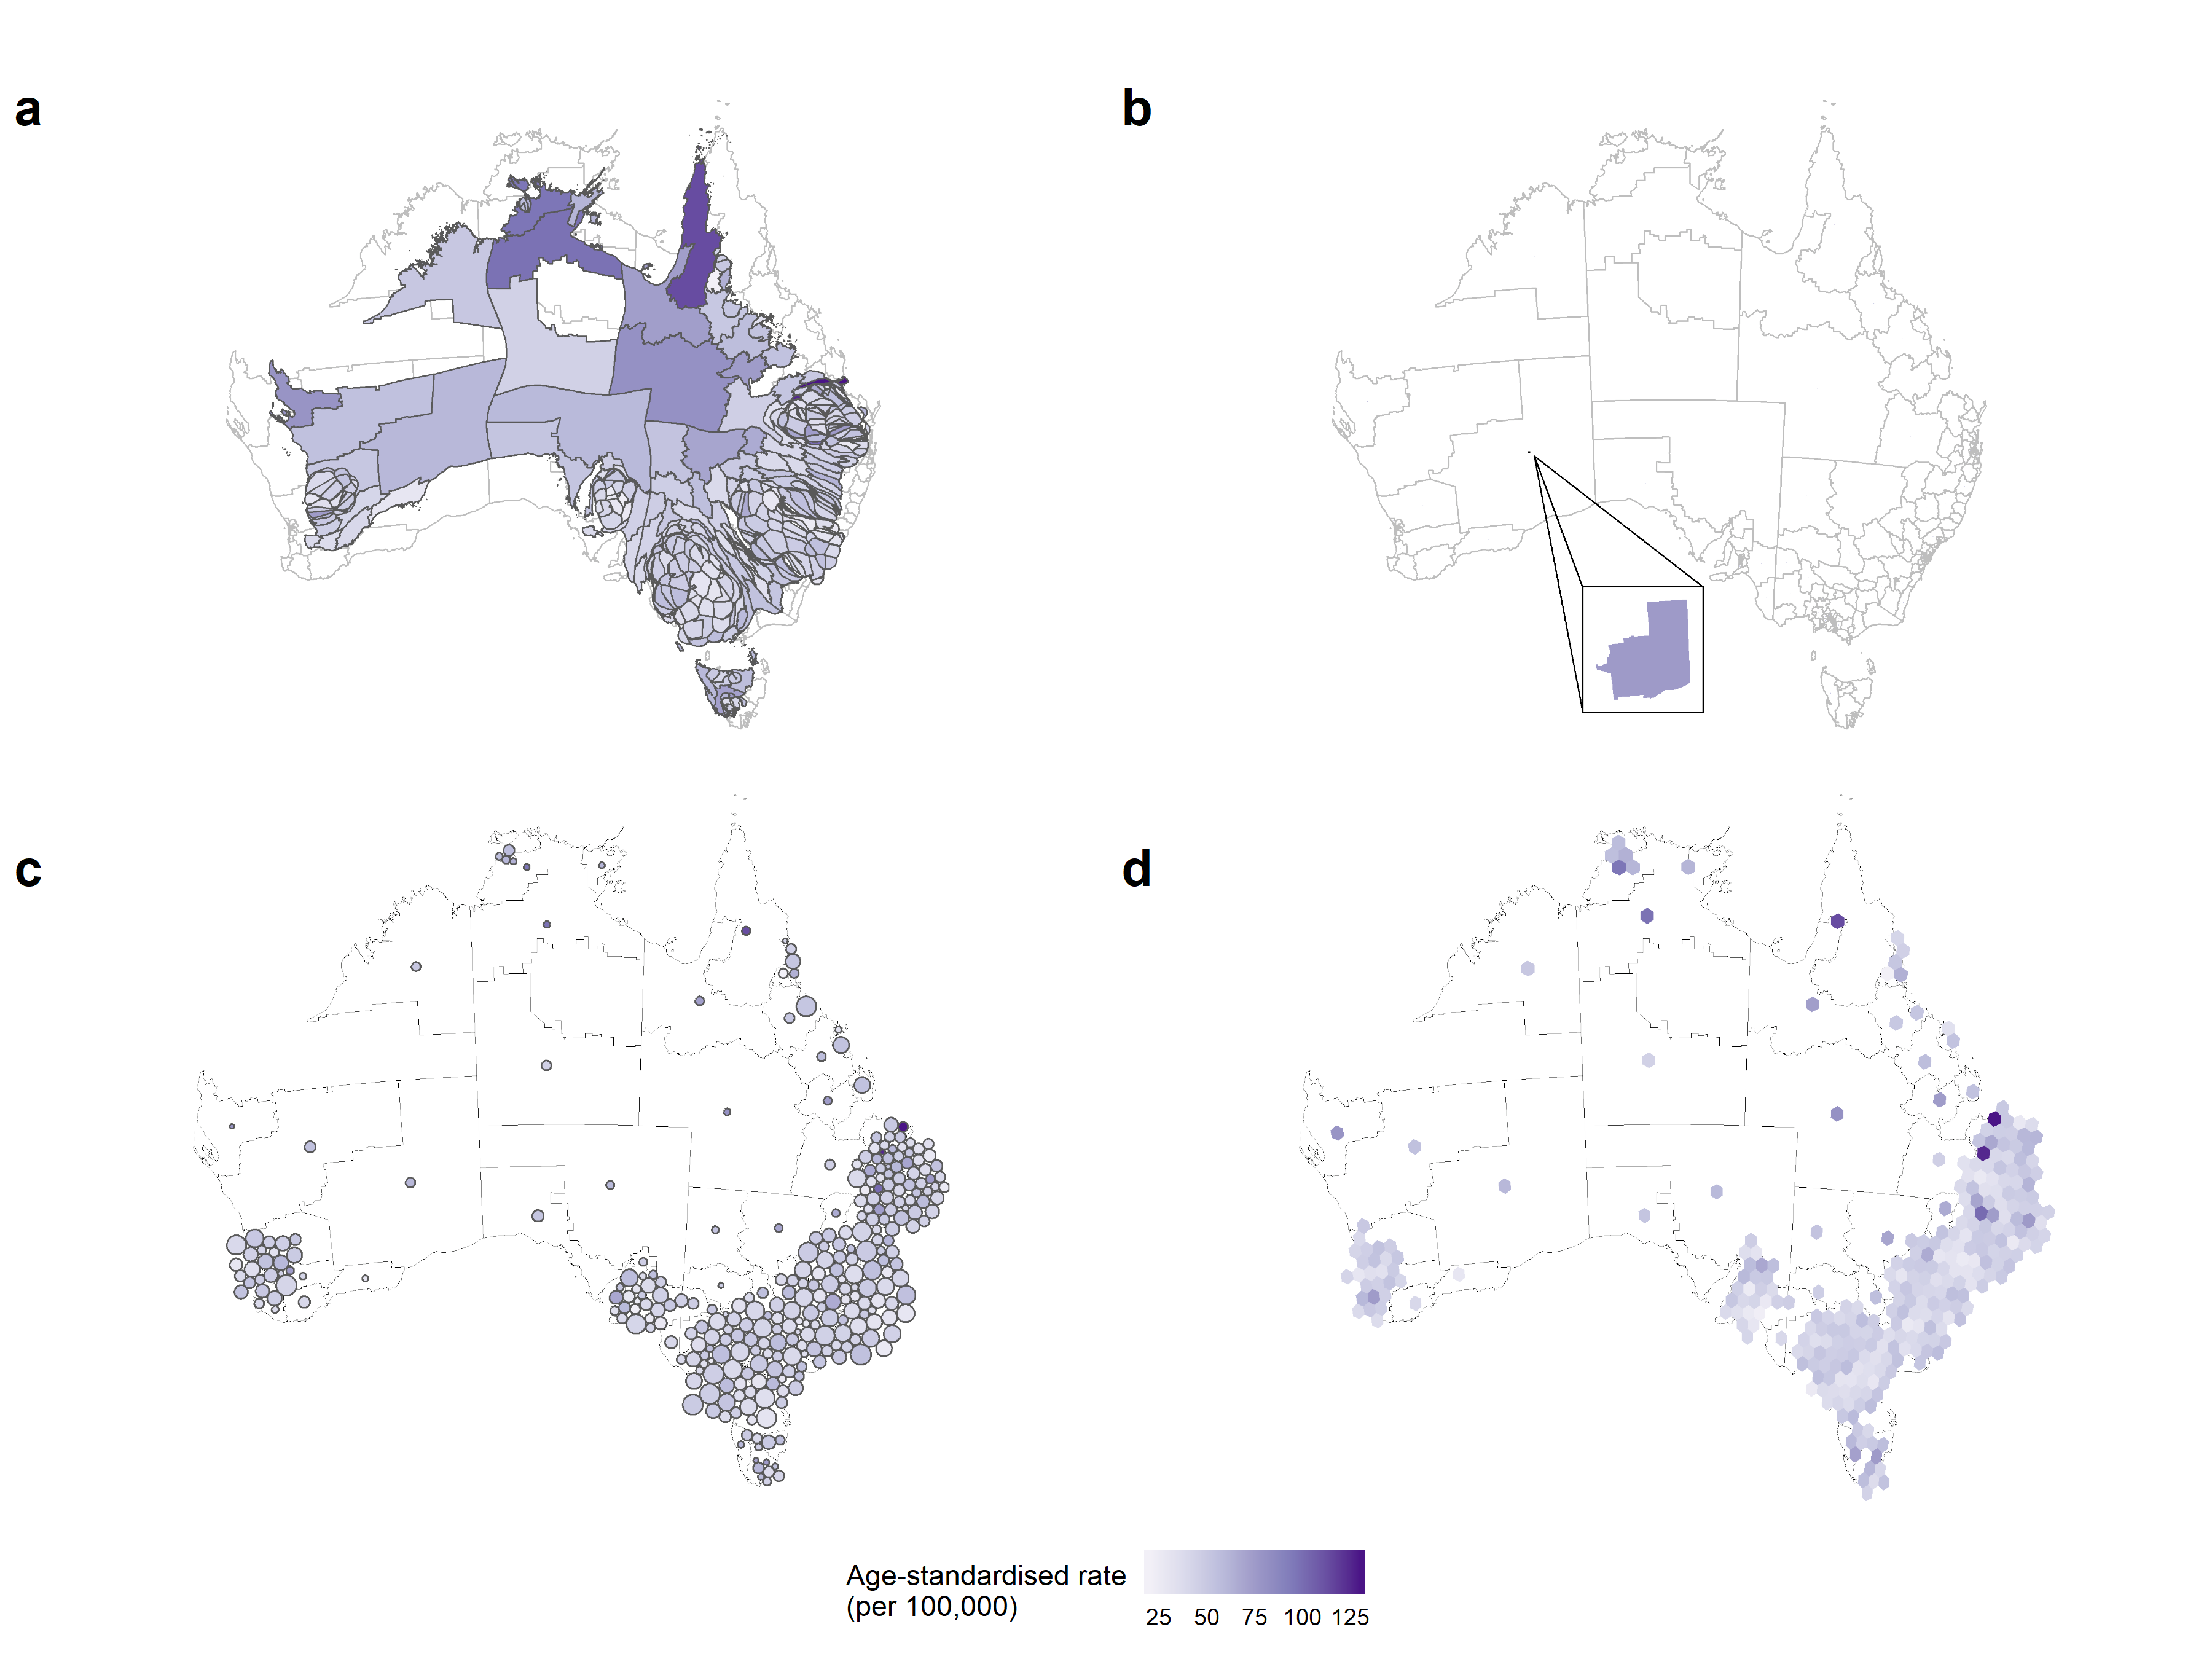
\includegraphics[width=50in]{figures/02-literature/auscartograms} \caption{ Cartograms showing melanoma incidence in Australia: (a) contiguous, partially population transformed, (b) non-contiguous shape preserved, (c) Dorling, (d) hexagon tile map. The contiguous cartogram has expanded the highly populated areas while preserving the full shapes of rural areas. If it accurately sized areas by population, the country would be unrecognizable. The shape-preserved is unreadable due to the small area sizes. The Dorling cartogram presents all areas but many are difficult to compare. The hexagon tile map provides a reasonable spatial distribution despite having isolated hexagons in the outback areas.}\label{fig:auscartograms}
\end{figure}

\hypertarget{neither-choropleth-maps-or-cartograms-perform-well-for-australia}{%
\subsection{Neither choropleth maps or cartograms perform well for Australia}\label{neither-choropleth-maps-or-cartograms-perform-well-for-australia}}

Figure 4 shows four main types of cartograms using melanoma incidence on Australian Statistical Areas at Level 3 \autocite{abs2016}. The version of a contiguous cartogram (a) has expanded the highly populated areas while preserving the full shapes of rural areas. It has not fully resolved the population transformation of areas, and if it had accurately sized areas by population, the country would be unrecognizable. The shape-preserved cartogram is unreadable, and it has reduced all areas to tiny spots on the map. Zooming in on a high-resolution output shows it does preserve the shapes. The Dorling cartogram and the hexagon tile map provide reasonable displays of the spatial distribution, despite having too much white-space in the outback areas.

\hypertarget{limitations-of-alternative-displays}{%
\subsection{Limitations of alternative displays}\label{limitations-of-alternative-displays}}

Cartograms provide the spatial distortion to more accurately convey the statistical distribution, focusing on the human impact of the disease. However, the transformation of contiguous cartograms often occurs at the expense of the shape of areas \autocite{CBATCC}, {[}\textcite{NAC}, \autocite{TAAM}. When the population density of the geographic units is highly dissonant with geographic density, the cartogram will lose all spatial context. Dorling \autocite{ACTUC} has a cartogram showing the 1966 general election results, which looked very little like the geographical shape of Australia.

Some mix of tiling, faceting or even micromaps, which allow some spatial continuity while also zooming into small areas, are good solutions for difficult geographies. Table 3 summarizes the key criteria for testing maps and alternative displays. Moore and Carpenter \autocite{SAMGIS} and Bell et al.~\autocite{CPISACA} provide suggestions and comments to help map creators best communicate their health data and spatial analysis.

Table 4: Summary of features and constraints of common mapping methods used to display cancer statistics (Y=Yes, N=No, S=Sometimes).

\begin{longtable}[]{@{}lcccccc@{}}
\toprule
& Choropleth & Contiguous & Non-contig & Dorling & Tile maps & Geofacets\tabularnewline
\midrule
\endhead
Spatial distortion & N & Y & Y & Y & Y & Y\tabularnewline
Preserves neighbors & Y & Y & Y & S & S & S\tabularnewline
Conceals small areas & Y & S & N & N & N & N\tabularnewline
Uniform shape & N & N & N & Y & Y & Y\tabularnewline
Univariate only & Y & Y & Y & S & S & N\tabularnewline
Manual construction & N & N & N & N & Y & Y\tabularnewline
\bottomrule
\end{longtable}

\hypertarget{ch:interacting}{%
\section{User interaction}\label{ch:interacting}}

One of the concerns of adding too much information to a map is the fear of cognitive overload \autocite{mcgranaghan1993cartographic} in which the user reaches an information threshold, beyond which they become confused. It can be a juggling act for a diverse audience, with experts probably preferring more detail \autocite{cliburn2002design} while a simpler display is more broadly readable. Interactivity is a design feature within modern mapping methods that can be used to incorporate additional information and complexity without overloading the user. Effective user-centred interactive actions produce rapid, incremental, and reversible changes to the display \autocite{DMIV}.

Monmonier \autocite{HTLWM} says that interactivity can be used to allow users to explore the map for more information and provides flexibility for the display. The user can toggle between different variables, map views or even multiple realizations of future scenarios \autocite{goodchild1994introduction}. This provides additional mechanisms for the users to digest the uncertainty of the available information \autocite{maceachren1992visualizing}, \autocite{van1994visualization}. When the needs of the audience are changeable and are also the priority, the map creator can allow interactivity for map users to explore a data set through dynamic interactions. This can allow inspection of the data from many views \autocite{DQBCM}. User interaction with maps helps to understand and interpret the spatial distribution of disease, to validate, explain or explore the presented statistics and their relationships to each other \autocite{TNTEA}.

Interactivity enables supplementary information to be incorporated into online atlases without cluttering the display. Interactive design features, found in online cancer maps, include tool tips, drop-down menus, data selection, zooming, and panning to allow users to explore the map as they want more information and allow flexibility in the display \autocite{HTLWM}. The use of these supports can be found in various online cancer maps and are shown in Figure 5 \autocite{roberts2019communication}.

Animation, in contrast to interactivity, usually involves pre-computing views and showing these in a sequence. Lin Pedersen \autocite{TGA} provides an overview of animation for maps using the R package \texttt{gganimate} \autocite{gganimate}. Animations are used to communicate a message by capturing and directing users' attention. It is most often employed to show changes over time. The controls for basic animation are usually placed outside of the plot space \autocite{TGA}, and the map image is updated/replaced as the animation progresses.

Weather maps are a thoroughly developed examples of animation of spatial displays to communicate information to the general public \autocite{CPISACA}. The movement of a weather system will follow a forecasted path. All map users can follow the animated path of the weather system across the geography over a specified period.

The Australian Cancer Atlas \autocite{TACA} provides \href{https://atlas.cancer.org.au/app/tour/lungcancer}{tours} that change the display to draw users' attention to areas on the map that are relevant to the story.
This implementation of animation gives users tools to plan their exploration.

\begin{figure}
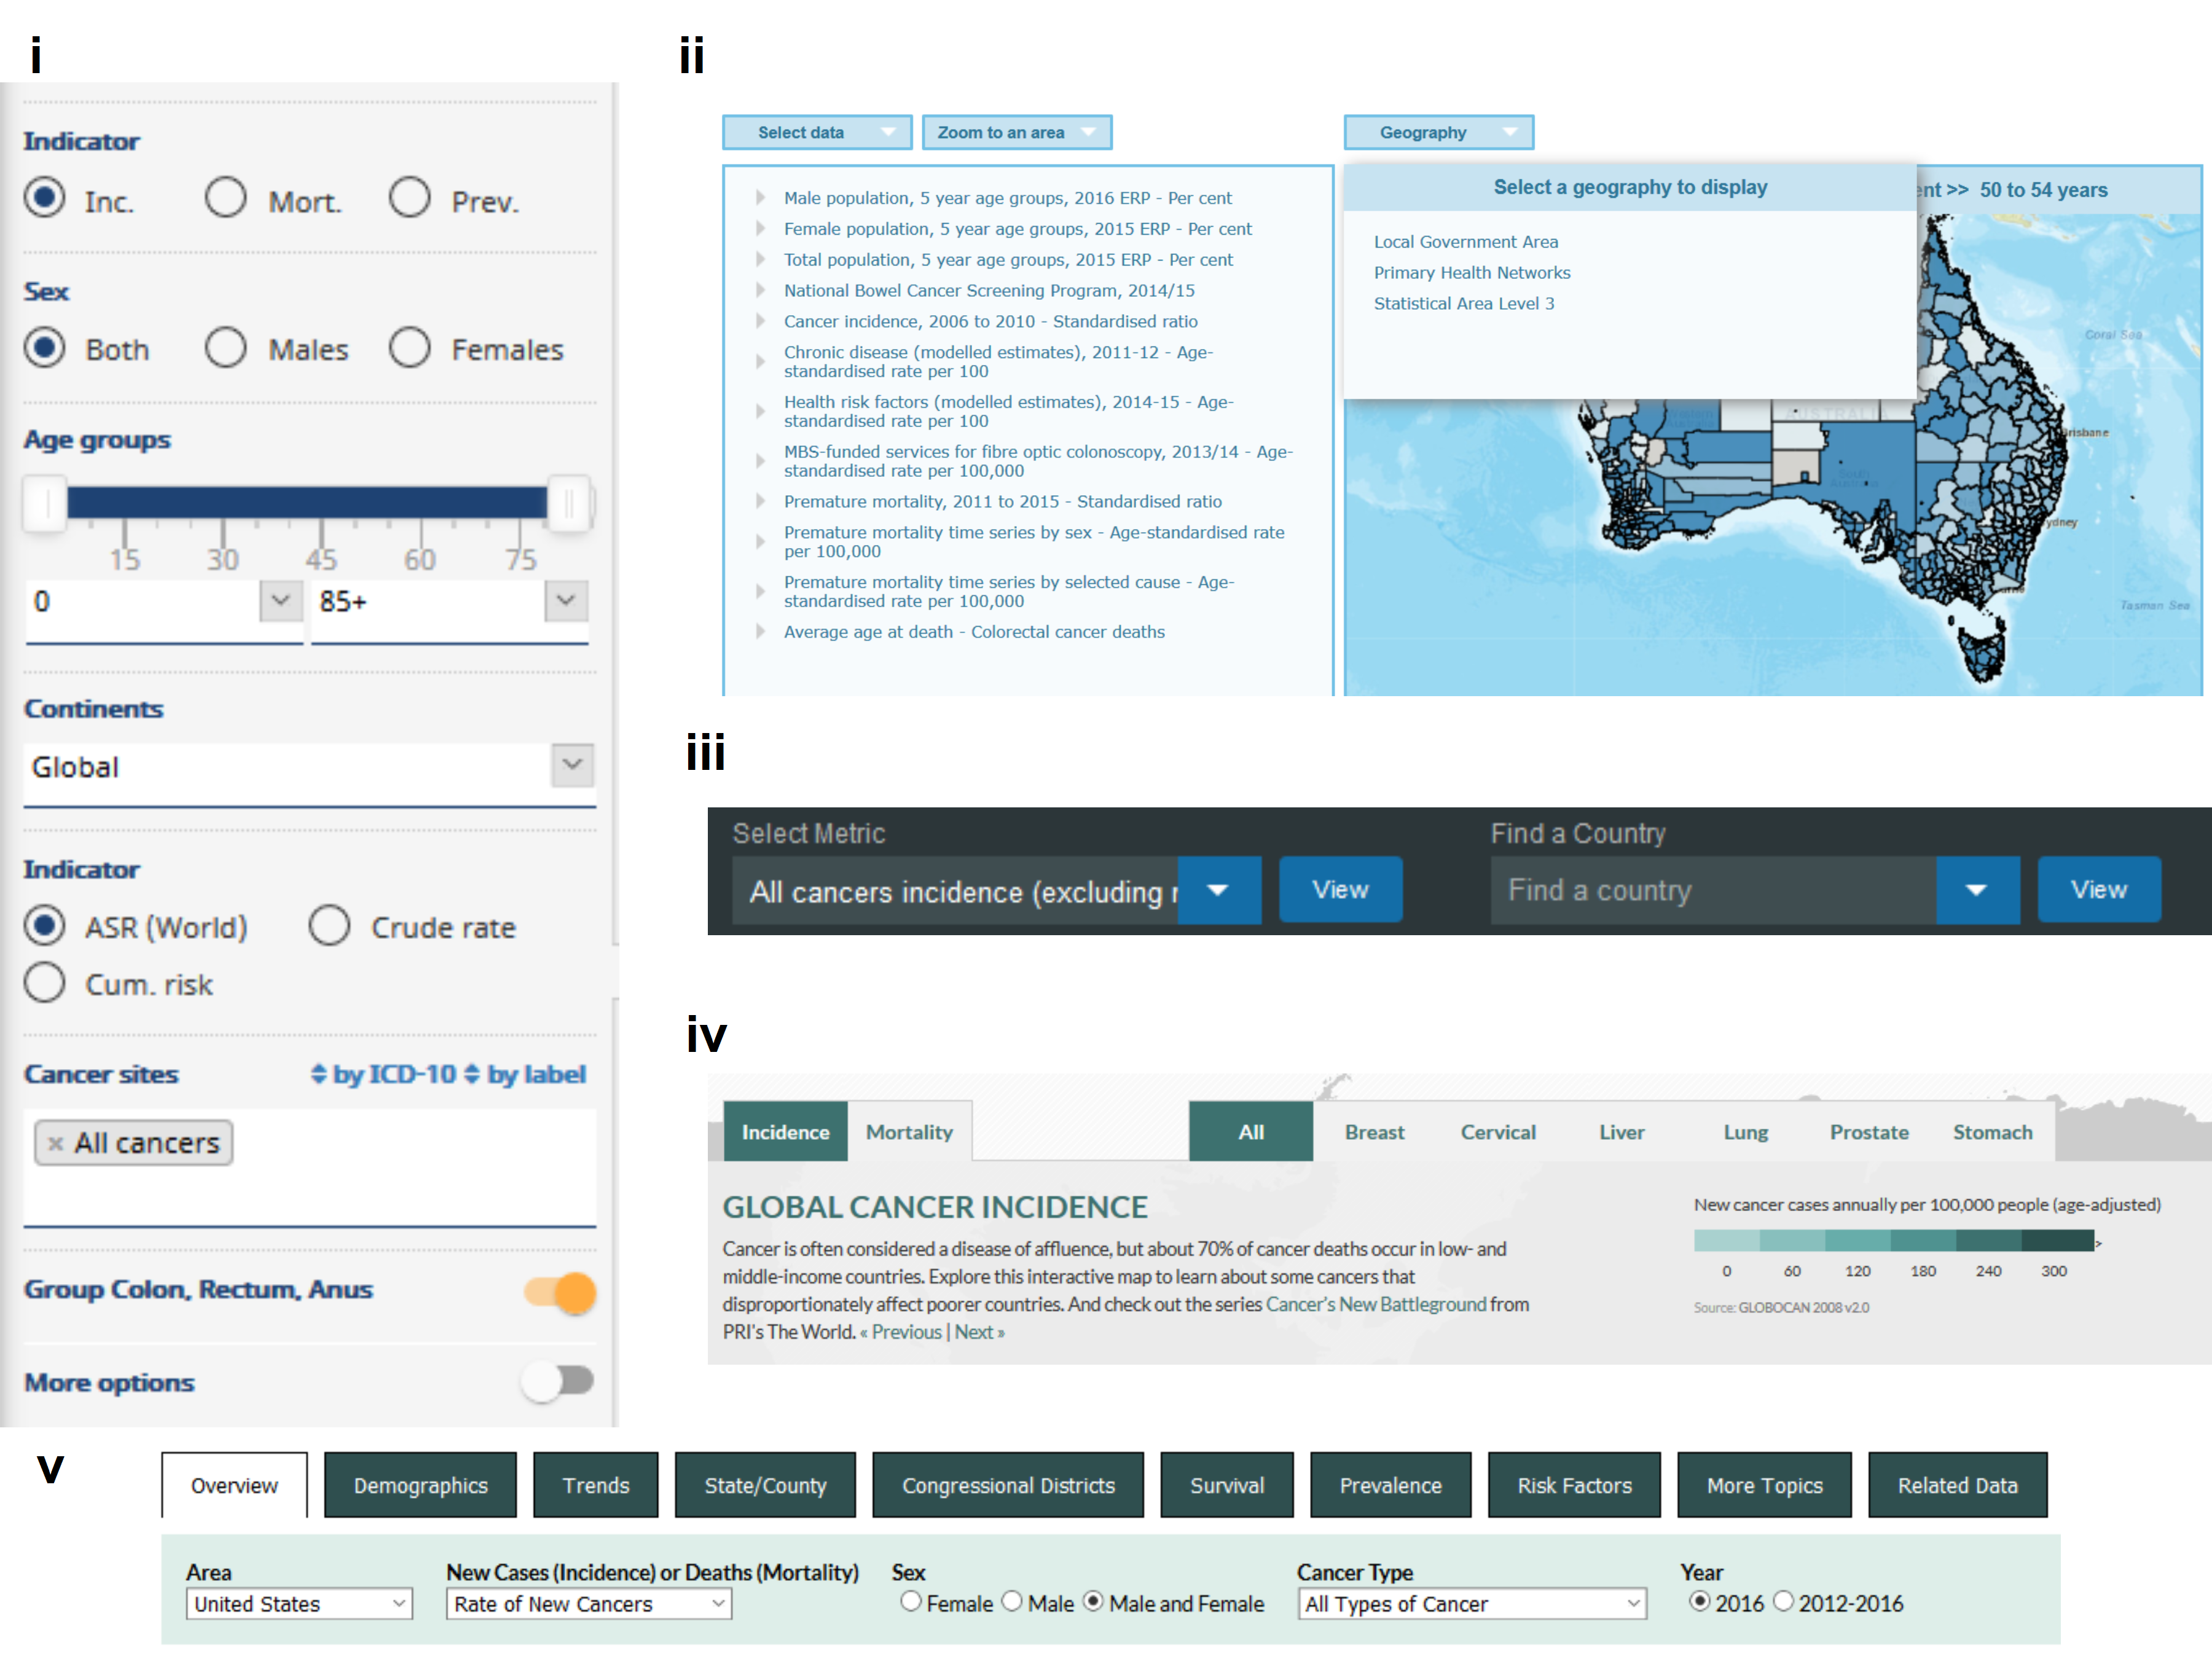
\includegraphics[width=50in]{figures/02-literature/interacting} \caption{ Interactive controls of displays in publicly available choropleth cancer maps: (i) GUI controls for statistic, sex, age groups, continents, and cancer types for Globocan 2018 [@Globocan], (ii) Menus for variable selection and zooming on Bowel Cancer Australia Atlas, (iii) Menus for choosing variables and countries in The Cancer Atlas, (iv) Tabs for different indicators and cancer types in Global Cancer Map, (v) Menus and toggles for variable and subset selection in United States Cancer Statistics: Data Visualizations.}\label{fig:interacting}
\end{figure}

Figure 6 shows two examples of more sophisticated interactive maps. The Spanish Cancer map (left) contains a linked display between a choropleth map and time series plots of cancer change. In linked plots, changing values in one display will trigger changes of corresponding elements in another display. Here, the temporal change in the choropleth map can be played out as an animation. Mousing over the time series plots will highlight the line for a particular region. The Canadian Breast Cancer Mortality map (right) has a magnifying glass that allows the user to zoom into small areas. It is easy to control and shows precise details in small areas.

\begin{Shaded}
\begin{Highlighting}[]
\NormalTok{knitr}\OperatorTok{::}\KeywordTok{include_graphics}\NormalTok{(}\StringTok{"figures/02-literature/animating.png"}\NormalTok{)}
\end{Highlighting}
\end{Shaded}

\begin{figure}
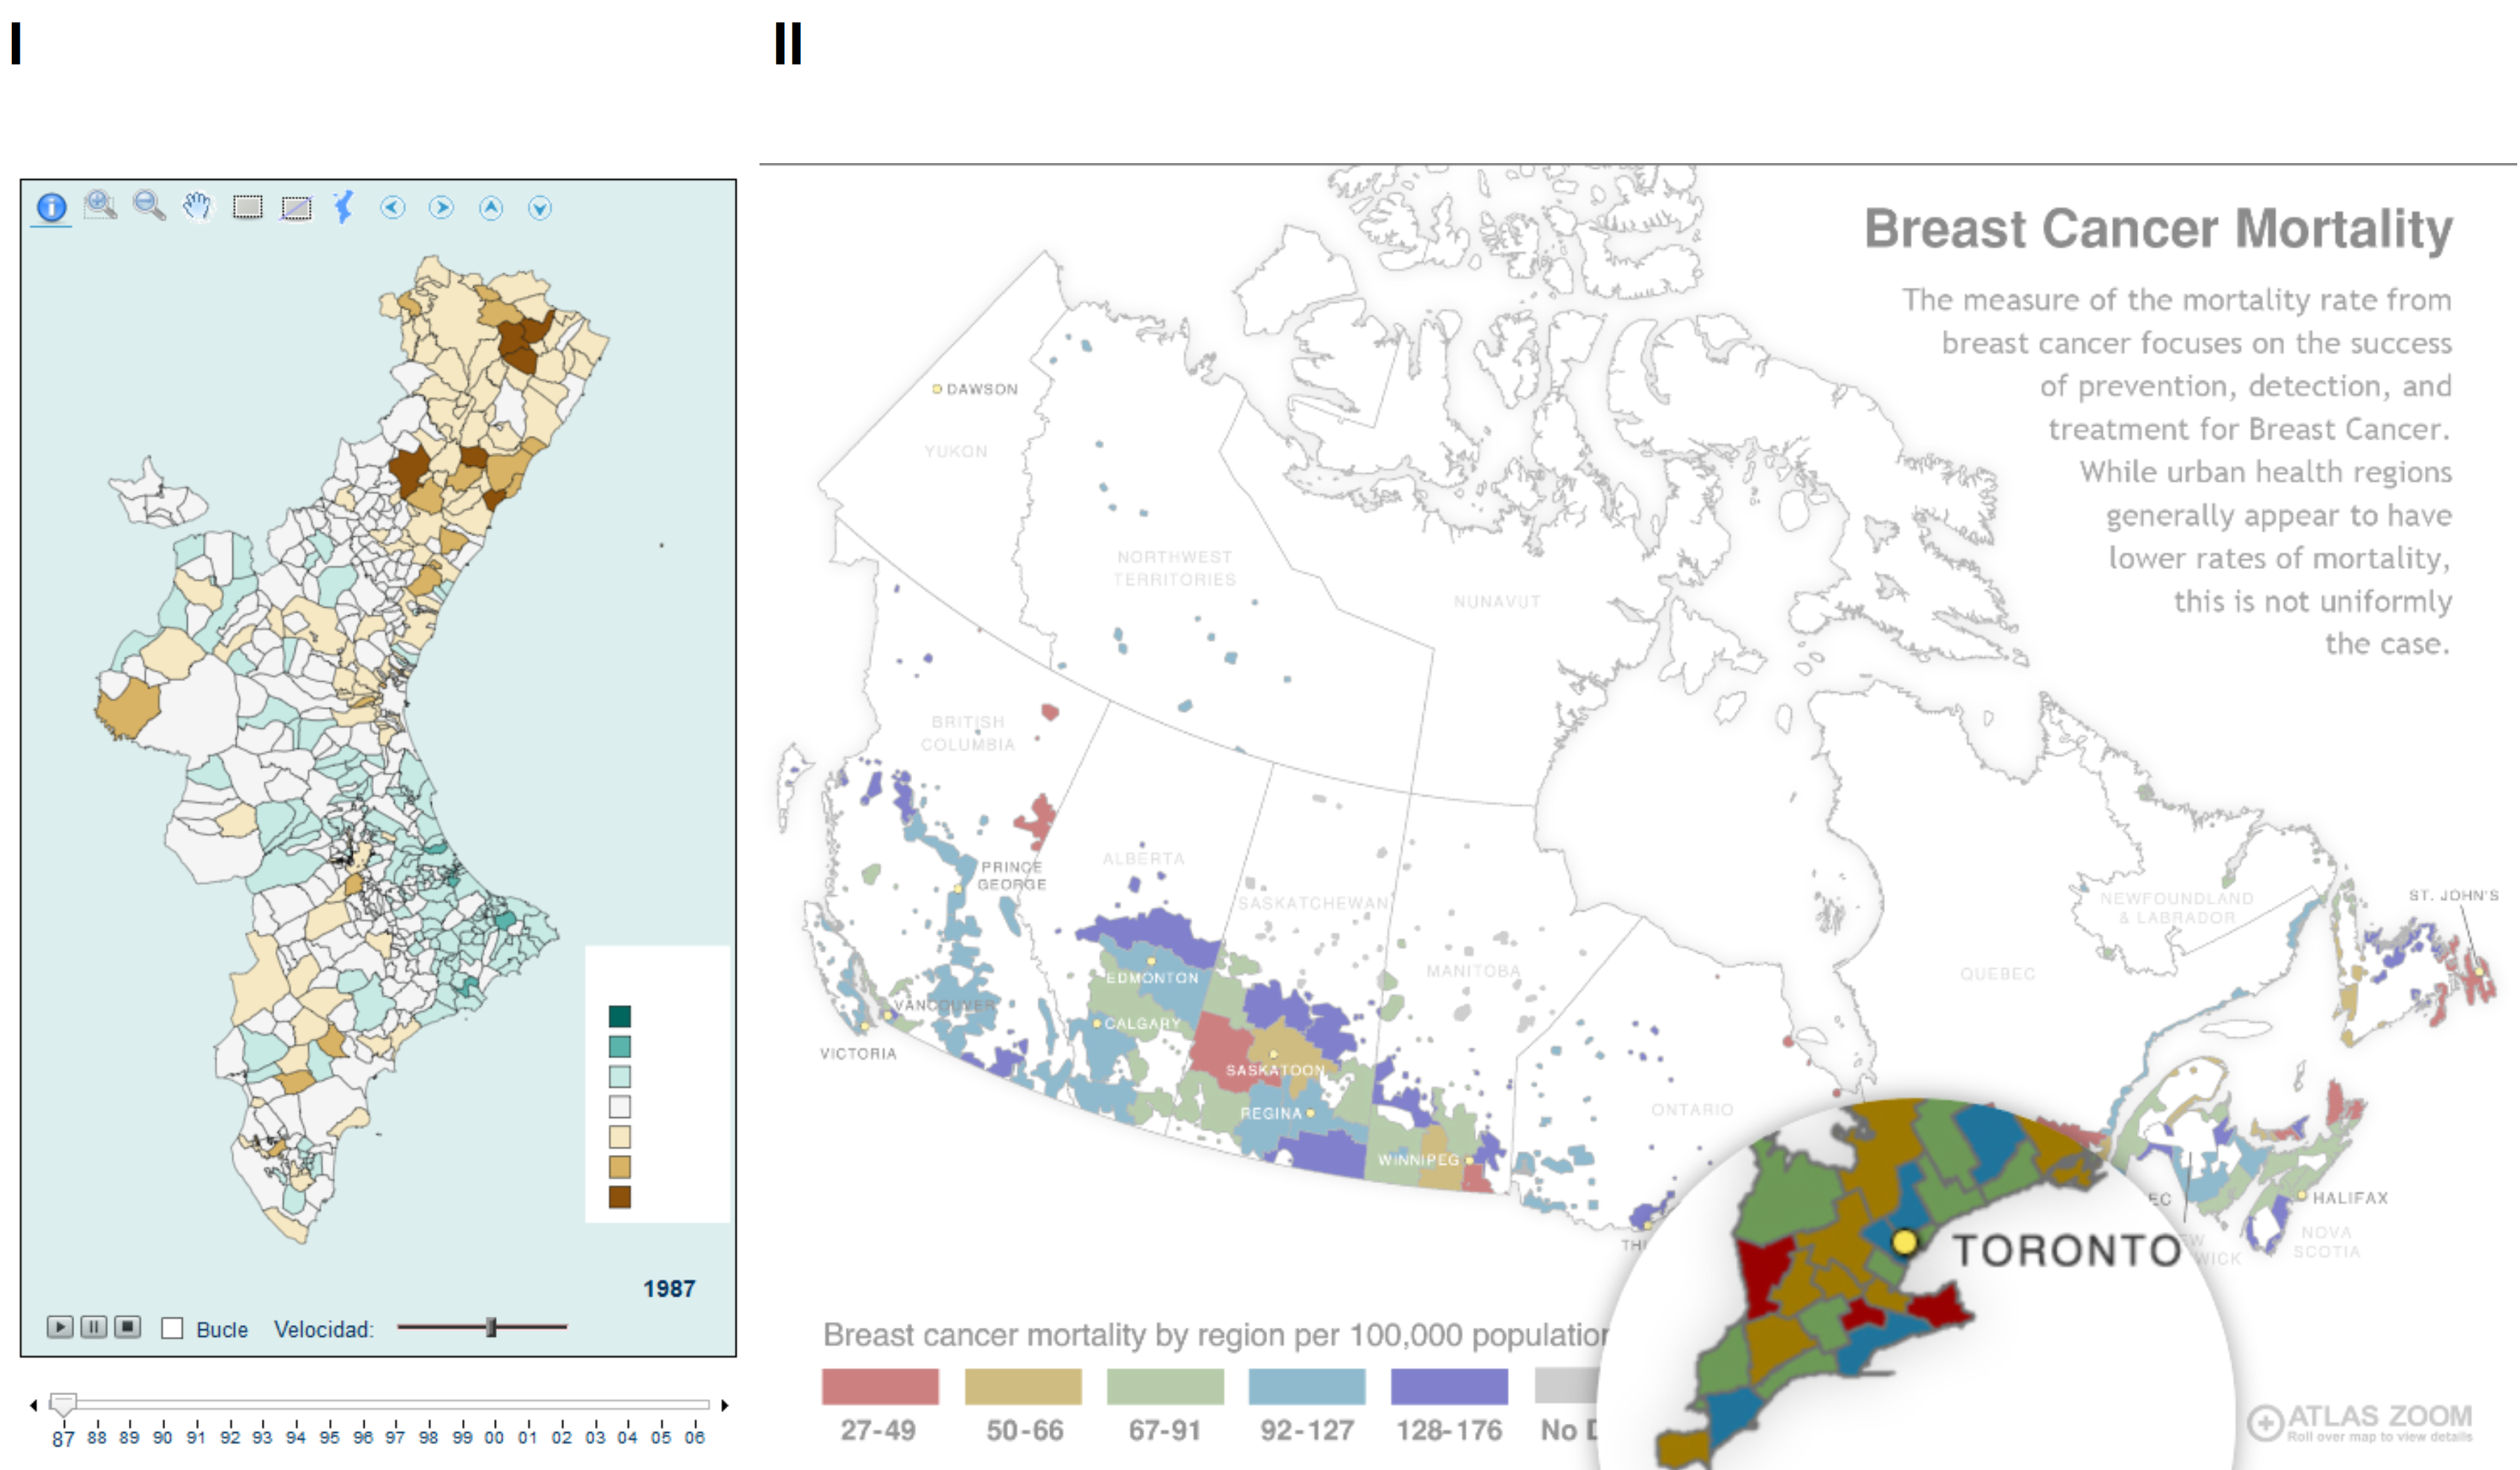
\includegraphics[width=50in]{figures/02-literature/animating} \caption{Two examples of advanced interactivity (and animation) in publicly available choropleth cancer maps: a. Linked maps and time-series line plots, with temporal animation in Map of Cancer Mortality Rates in Spain, b. A highly responsive magnifying glass on a map of Breast Cancer Mortality in Canada.}\label{fig:animating}
\end{figure}

\hypertarget{conclusions}{%
\section{Conclusions}\label{conclusions}}

This paper provides an overview of mapping practices as commonly used for cancer atlases and recommends new approaches, such as cartograms and hexagon tile maps that should be adopted going forward. The conventional approach is the choropleth map, and it is widely used. The choropleth map suffers when there are small geographic units, as occurs in Australia where the population is concentrated on the coast, the information about the burden of cancer on those communities can be hidden. Making an inset can clarify congested regions but this breaks the viewers' attention as they shift focus from the map to the inset, and if there are many congested areas, many insets would be needed. The map alternatives implement trade-offs between the familiar shapes, and the importance of the geographic areas in the context of the areas. Given the population or a cancer statistic for each area, the geographic size or shape will change. Alternative displays allow the spatial distribution of cancer data to be digested by map users.

Many statistics are commonly used in cancer displays. The most basic is the incidence rate. It is common to see relative rates which measure how far a region is above or below the average. The purpose of using a relative rate is, perhaps the desire to pinpoint the areas that need attention because they have higher than expected rates.
A region might be much higher than average, but it may not be close to a health concern, because all regions have a low incidence. Supplementary materials can allow map users to recognise when this occurs.

Interaction with maps is an important component of public atlases, and is easy to add with today's technology. The purpose is to provide access to more information than is possible to display in a single map, without overwhelming the viewer. Too many choices can similarly overwhelm a viewer, and thus decisions do need to be made about content to provide for accurate and comprehensive communication of information. Similarly, providing ways for users to interact with the display encourages engagement, and creative, efficient, elegant, interactive tools elicit curiosity about the data.

\hypertarget{ch:algorithm}{%
\chapter{An Algorithm For Spatial Mapping Using a Hexagon Tile Map, With Application to Australian Maps}\label{ch:algorithm}}

This chapter relates to the first research aim as stated in Section \ref{sec:aims}.
The chapter introduces the step devised for the algorithm.
The chapter frames the steps in light of the \texttt{sugarbag} \autocite{sugarbag} package functions that allow users to enact the algorithm in \texttt{R} \autocite{R}. It uses the Statisical Areas of Australia at Level 2, taking a subset and considering only those located within the island of Tasmania.
It also provides an example of how to animate between the choropleth map display and the hexagon tile map.

This chapter was submitted for publication to the \emph{Journal of Statistical Software} for publication.
The steps in this algorithm are implemented in the \texttt{sugarbag} \autocite{sugarbag} package for \texttt{R} \autocite{R}.

\includepdf[pages = {1-}, scale=0.8]{statement-of-contribution_algorithm.pdf}

\hypertarget{abstract-2}{%
\section*{Abstract}\label{abstract-2}}
\addcontentsline{toc}{section}{Abstract}

This algorithm creates a tesselated hexagon display to represent each of the spatial polygons. It allocates these hexagon in a manner that preserves the spatial relationship of the geographic units. It showcases spatial distributions, by emphasising the small geographical regions that are often difficult to locate on geographic maps. Spatial distributions have been presented on alternative representations of geography for many years. In modern times, interactivity and animation have begun to play a larger role, as alternative representations have been popularised by online news sites, and atlas websites with a focus on public consumption. Applications are increasingly widespread, especially in the areas of disease mapping, and election results.

\hypertarget{introduction-1}{%
\section{Introduction}\label{introduction-1}}

The current practice for presenting geospatial data is a choropleth map display. These maps highlight the geographic patterns in geospatially related statistics \autocite{SAMGIS}.
The land on the map space is divided into geographic units, these boundaries are usually administrative, such as states or counties. The units are filled with colour to represent the value of the statistic \autocite{EI}.

Australian residents are increasingly congregating around major cities, the vast rural areas are often sparsely populated in comparison to the urban centres.
In Australia, government bodies such as the Australian Bureau of Statistics (ABS), and the Australian Electoral Commission (AEC) hold the responsibility for the division of the population into geographic units. If it necessary, the AEC may adjust the boundaries of the areas as the population increases. The division of the population into approximately equal population areas results in dramatically different square meterage of the geographic areas. This can give unequal attention to the statistic of each area, this can cause misrepresentation of the spatial distributions of human related statistics in geographic maps.

The solutions to this visualisation problem begin with the geography. Cartograms apply a transformation to the geographic boundaries based on the value of the statistic of interest. These displays result in a distortion of the map space to represent differences in the statistic across the areas \autocite{ACCAC}.
The statistic of interest is used to determine the cartogram layout. When the
Australian population is the statistic of interest, the result is a population cartogram. They fail to preserve a recognisable display due to the difference in size of metropolitan and rural areas \autocite{ACTUC}, \autocite{GOINO}.
Contiguous cartograms change the shape of areas, while preserving boundary relationships of neighbours. Non-contiguous cartograms maintain the geographic shape of each geographic area, but will lose the connection to neighbours as the polygon for each geographic area shrinks or grows.

Alternative maps shift the focus from land area and shape, to the value of the statistics in a group of areas.
Alternative mapping methods allow increased understanding of the spatial distribution of a variable across the population, by fairly representing each administrative area. This acknowledges that the amount of residents can be different but recognises that each area, or person within it is equally important.

tile maps, Rectangular cartograms \autocite{ORC} and Dorling cartograms \autocite{ACTUC}, all use one simple shape to represent each area. They place various importance on the preservation of spatial relationships, but all decrease the emphasis on the size of the geographic areas. These alternative map displays focus on the relationship between neighbours, attempting to preserve connections, and disregard the unique shapes of the administrative boundaries.

The \texttt{sugarbag} package provides a new algorithm to create tesselated hexagon tile maps.
It emphasises the capital cities as population hubs, and emphasises the distances rather than size of large, rural geographic units.

\hypertarget{algorithm}{%
\section{Algorithm}\label{algorithm}}

The algorithm presented in \texttt{sugarbag} package operates on a set of simple feature geometry objects, also known as \texttt{sf} \autocite{sf} polygons.

There are four steps performed to create a tesselated hexagon tile map.
These steps can be executed by the main function, \texttt{create\_hexmap}, or can be implemented separately for more flexibility. There are parameters used in the process that can be provided by users, if they are not, they will be automatically derived.

\begin{enumerate}
\def\labelenumi{\arabic{enumi}.}
\tightlist
\item
  Create the set of centroids to allocate
\item
  Create the grid of hexagons locations to use
\item
  Allocate each centroid to an available hexagon
\item
  Transform the data for plotting
\end{enumerate}

\hypertarget{parameters}{%
\subsubsection{Parameters}\label{parameters}}

The \texttt{create\_hexmap} function requires several parameters, if they are not provided, the information will be derived from the simple features (\texttt{sf}) set of shapes used. Users may choose to only use the \texttt{allocate} function when they wish to use a set of centroids, rather than \autocite{sf} polygons.

The following parameters must be provided to `create\_hexmap\}:

\begin{itemize}
\tightlist
\item
  \emph{shp:} an sf object containing the polygon information
\item
  \emph{sf\_id:} name of a column that distinguishes unique areas
\item
  \emph{focal\_points:} a data frame of reference locations used to allocate hexagons
\end{itemize}

\hypertarget{polygon-set}{%
\subsubsection{Polygon set}\label{polygon-set}}

The polygon set of Statistical Areas at Level 2 (SA2) \autocite{abs2016} of Tasmania in 2016 is provided with the \texttt{sugarbag} package as \texttt{tas\_sa2}.
A single column of the data set is used to identify the unique areas.
In this case, the unique SA2 names for each SA2 have been used.

The longitude and latitude centre of the capital cities of Australia are used as focal points to allocate each geographic area around the closest capital city. Hobart will be the common focal point, as this example uses only the areas in the state of Tasmania.

\begin{Shaded}
\begin{Highlighting}[]
\KeywordTok{data}\NormalTok{(capital_cities)}
\end{Highlighting}
\end{Shaded}

The following parameters will be determined within \texttt{create\_hexmap} if they are not provided. They are created as they are needed throughout the following example:

\begin{itemize}
\tightlist
\item
  \emph{buffer\_dist:} a float value for distance in degrees to extend beyond the geometry provided
\item
  \emph{hex\_size:} a float value in degrees for the diameter of the hexagons
\item
  \emph{hex\_filter:} amount of hexagons around centroid to consider for allocation
\item
  \emph{width:} the angle used to filter the grid points around a centroid
\end{itemize}

\hypertarget{create-the-set-of-centroid-points}{%
\subsubsection{Create the set of centroid points}\label{create-the-set-of-centroid-points}}

A set of centroids may be used directly. The set of polygons should be provided as an \texttt{sf} object, this is a data frame containing a \texttt{geometry} column. The \texttt{read\_shape} function can assist in creating this object for use in \texttt{R}.

The centroids can be derived from the set of polygons using the \texttt{create\_centroids} function:

\begin{Shaded}
\begin{Highlighting}[]
\NormalTok{centroids <-}\StringTok{ }\KeywordTok{create_centroids}\NormalTok{(}\DataTypeTok{shp_sf =}\NormalTok{ tas_sa2, }\DataTypeTok{sf_id =} \StringTok{"SA2_NAME16"}\NormalTok{)}
\end{Highlighting}
\end{Shaded}

\begin{figure}[H]
\centering
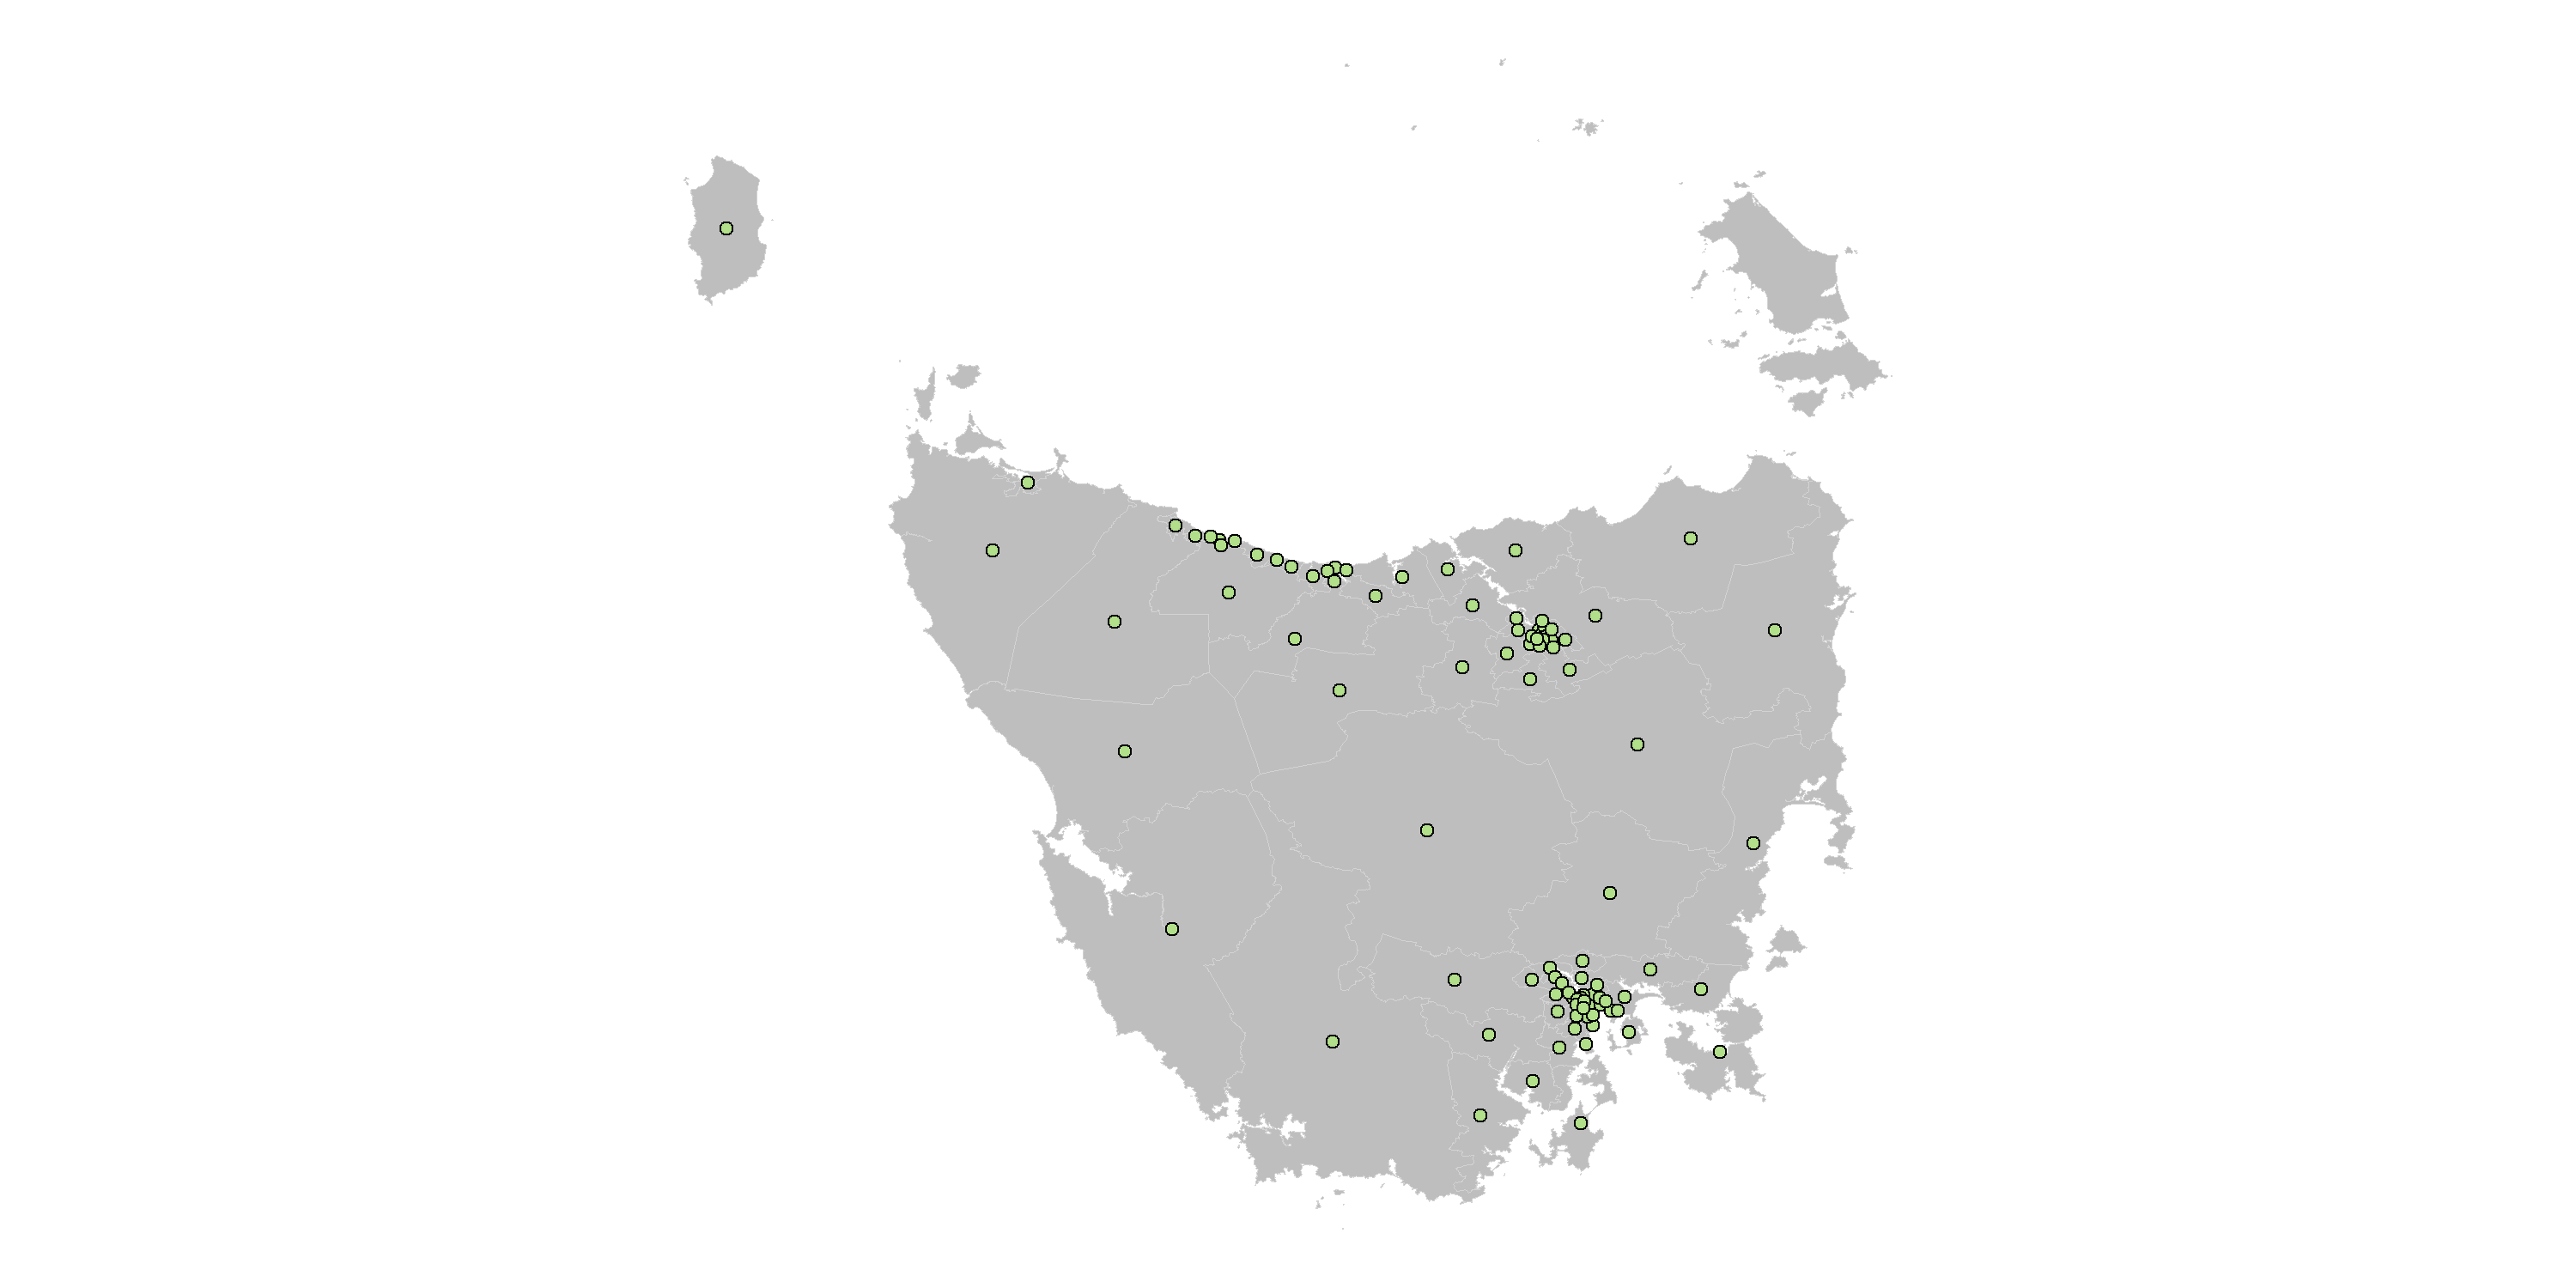
\includegraphics[width=16cm]{figures/03-algorithm/1centroids.png}
\caption{\label{fig:centroids_plot}The geographic shapes of the Statistical Areas of Tasmania at Level 2. The points show the locations of the centroids of the SA2 areas.}
\end{figure}

\hypertarget{create-the-hexagon-grid-points}{%
\subsubsection{Create the hexagon grid points}\label{create-the-hexagon-grid-points}}

A grid is created to ensure tessellation between the hexagons that represent the geographic units on a hexagon tile map.

The grid of possible hexagon locations is made using the \texttt{create\_grid} function.
It uses the centroids, the hexagon size and the buffer distance.

\begin{Shaded}
\begin{Highlighting}[]
\NormalTok{grid <-}\StringTok{ }\KeywordTok{create_grid}\NormalTok{(}\DataTypeTok{centroids =}\NormalTok{ centroids, }\DataTypeTok{hex_size =} \FloatTok{0.2}\NormalTok{, }\DataTypeTok{buffer_dist =} \FloatTok{1.2}\NormalTok{)}
\end{Highlighting}
\end{Shaded}

\hypertarget{step-1-creating-a-tesselated-grid}{%
\subparagraph{Step 1: Creating a tesselated grid}\label{step-1-creating-a-tesselated-grid}}

A set of longitude columns, and latitude rows are created to define the locations of the hexagons. The distance between each row and column is the size specified by \texttt{hex\_size}.
Equally spaced columns are created from the minimum longitude minus the buffer distance, up to the maximum longitude plus the buffer distance. Similarly, the rows are created from the latitude values and the buffer distance.
A unique hexagon location is created from all intersections of the longitude columns and latitude rows.
Figure \ref{fig:grid2} shows the original grid on the left, to allow for tessellating hexagons, every second latitude row on the grid is shifted right, by half of the hexagon size. The grid for tessellation is shown on the right.

\begin{figure}[H]
\centering
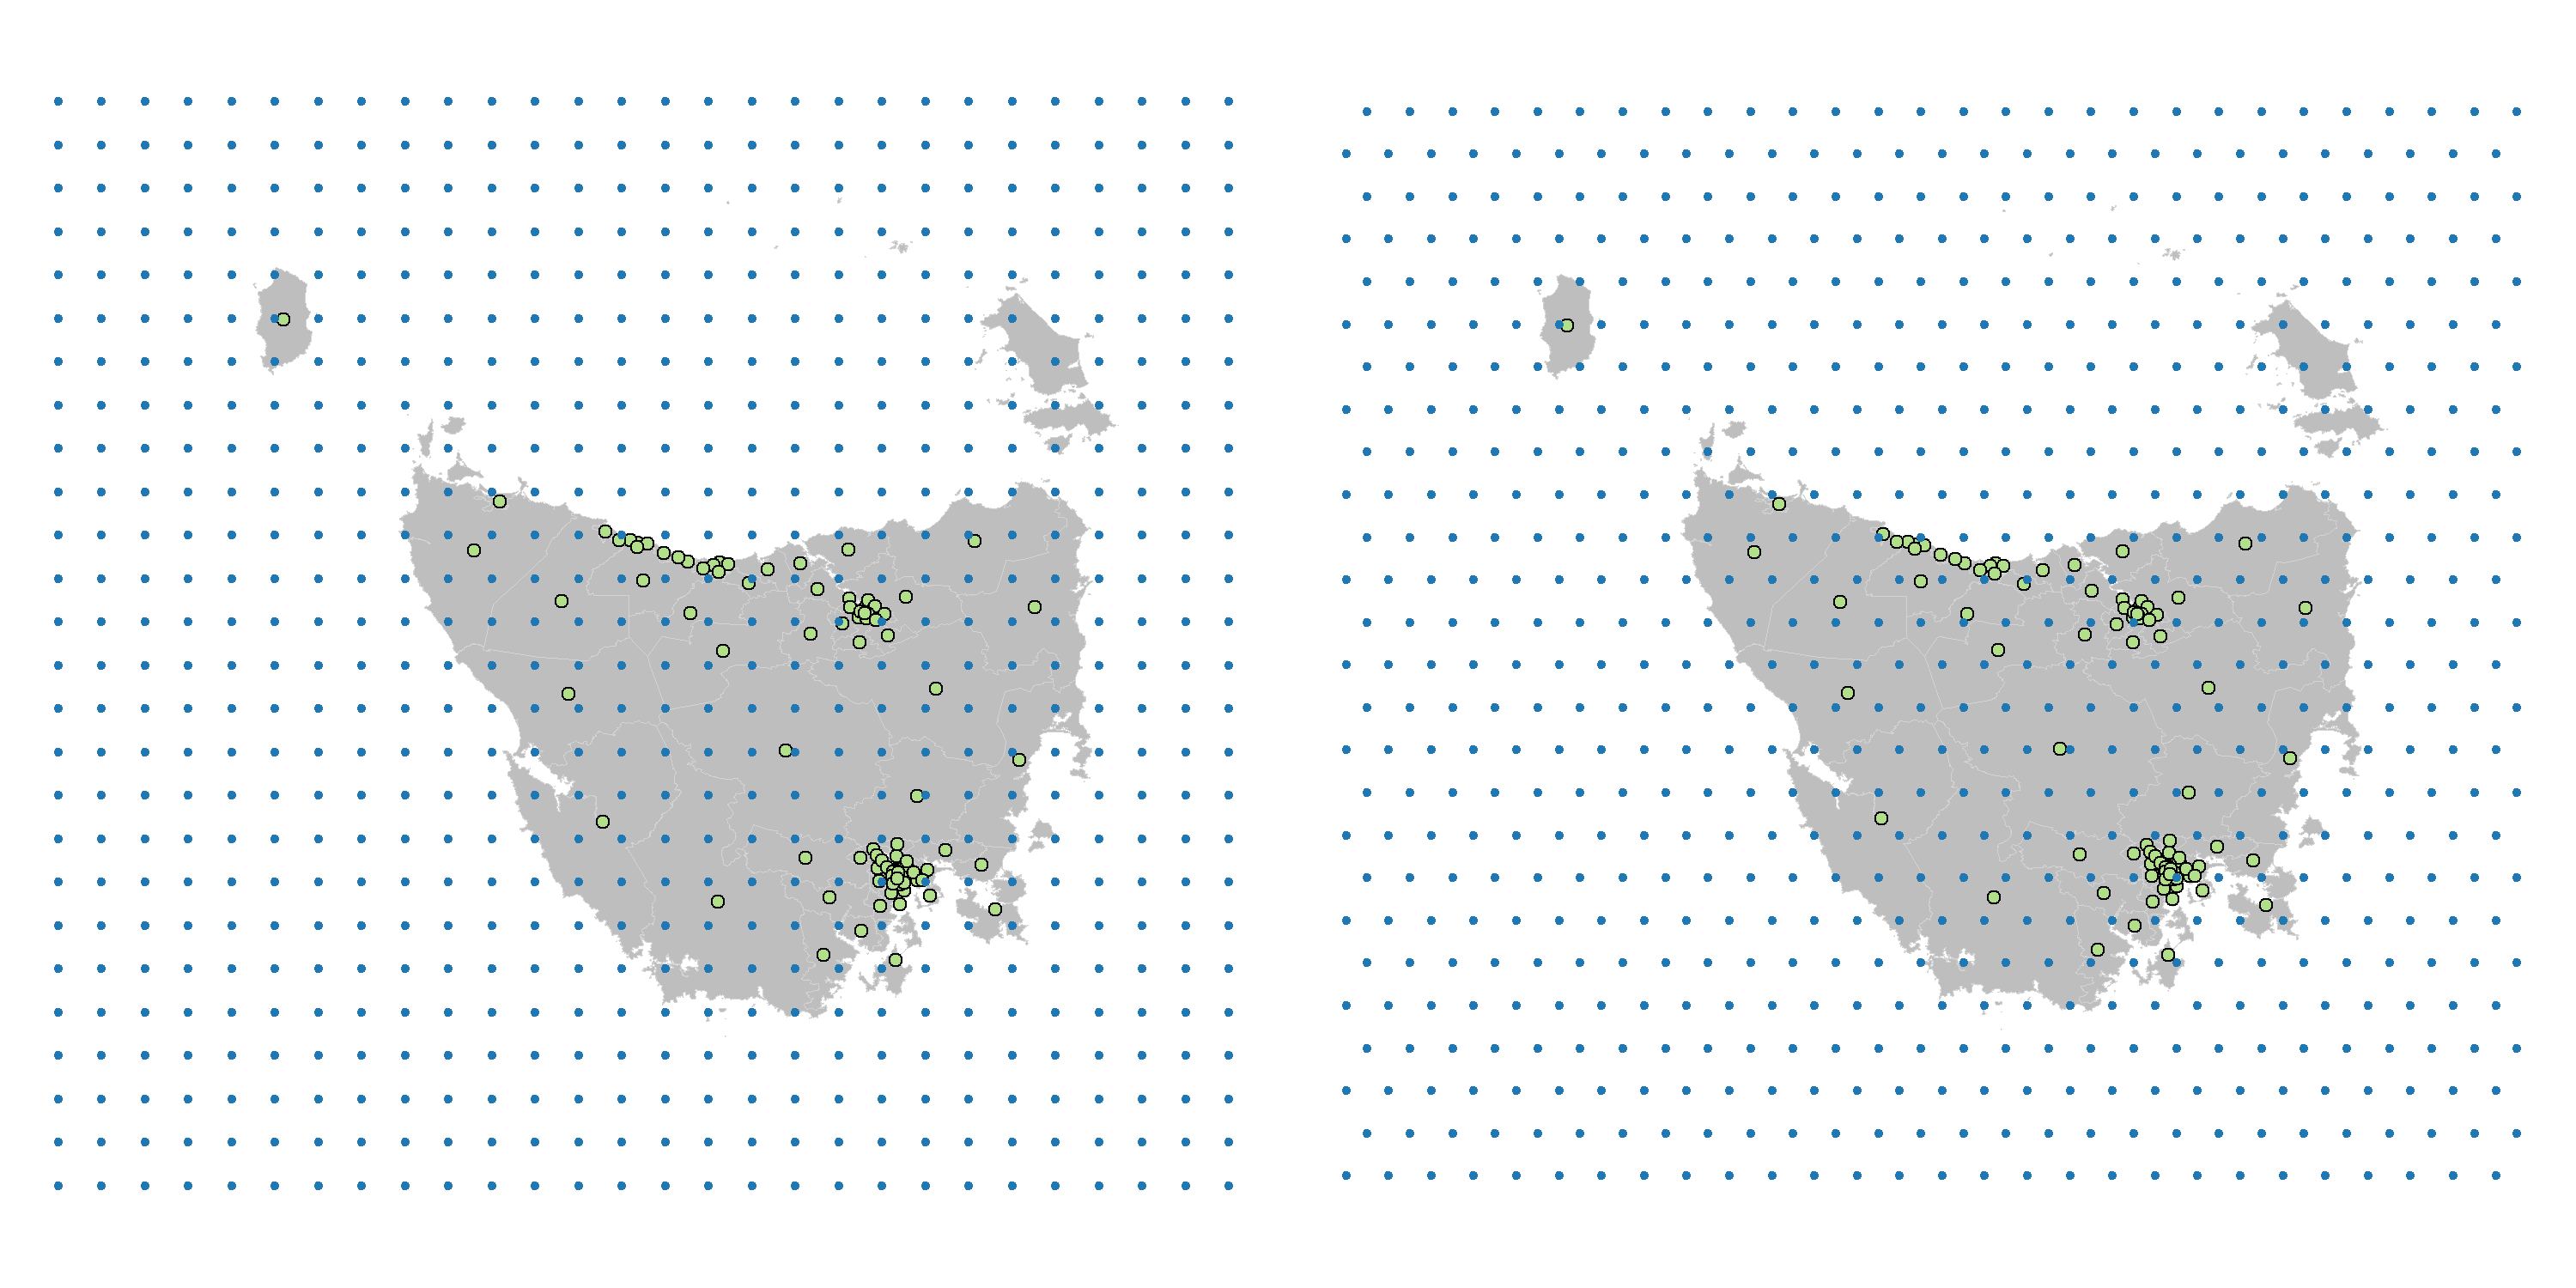
\includegraphics[width=16cm]{figures/03-algorithm/2grid.png}
\caption{\label{fig:grid2}Grid points to create a tile map.}
\end{figure}

\hypertarget{step-2-rolling-windows}{%
\subparagraph{Step 2: Rolling windows}\label{step-2-rolling-windows}}

Not all of the grid points will be used, especially if islands result in a large grid space.
To filter the grid for appropriate hexagon locations for allocation, the \texttt{create\_buffer} function is used by \texttt{create\_grid}.
It finds the grid points needed to best capture the set of centroids on a hexagon tile map.

The closest latitude row and longitude column are found for each centroid location. Then rows and columns of centroids are divided into 20 groups.
The amount of rows in each latitude group and the amount of columns in each longitude group are used as the width of rolling windows. The rolling windows can be seen on the bottom and right of the gris shown in Fig. \ref{fig:filter-grid}.
This will tailor the available grid points to those most likely to be used.
It also helps reduce the amount of time taken, as it decreases the amount of points considered for each centroid allocation.

The first rolling window function finds the minimum and maximum centroid values for the sliding window groups of longitude columns and the groups of latitude rows.

The second rolling window function finds the average of the rolling minimum and maximum centroid values, for the longitude columns and latitude rows.

\hypertarget{step-3-filtering-the-grid}{%
\subparagraph{Step 3: Filtering the grid}\label{step-3-filtering-the-grid}}

The grid points are kept only if they fall between the rolling average of the minimum and maximum centroid values after accounting for the buffer distance, for each row and column of the grid. The sparsely populated South-West region of National Park has much fewer points available compared to the South-East region containing the city of Hobart.

\begin{figure}[H]
\centering
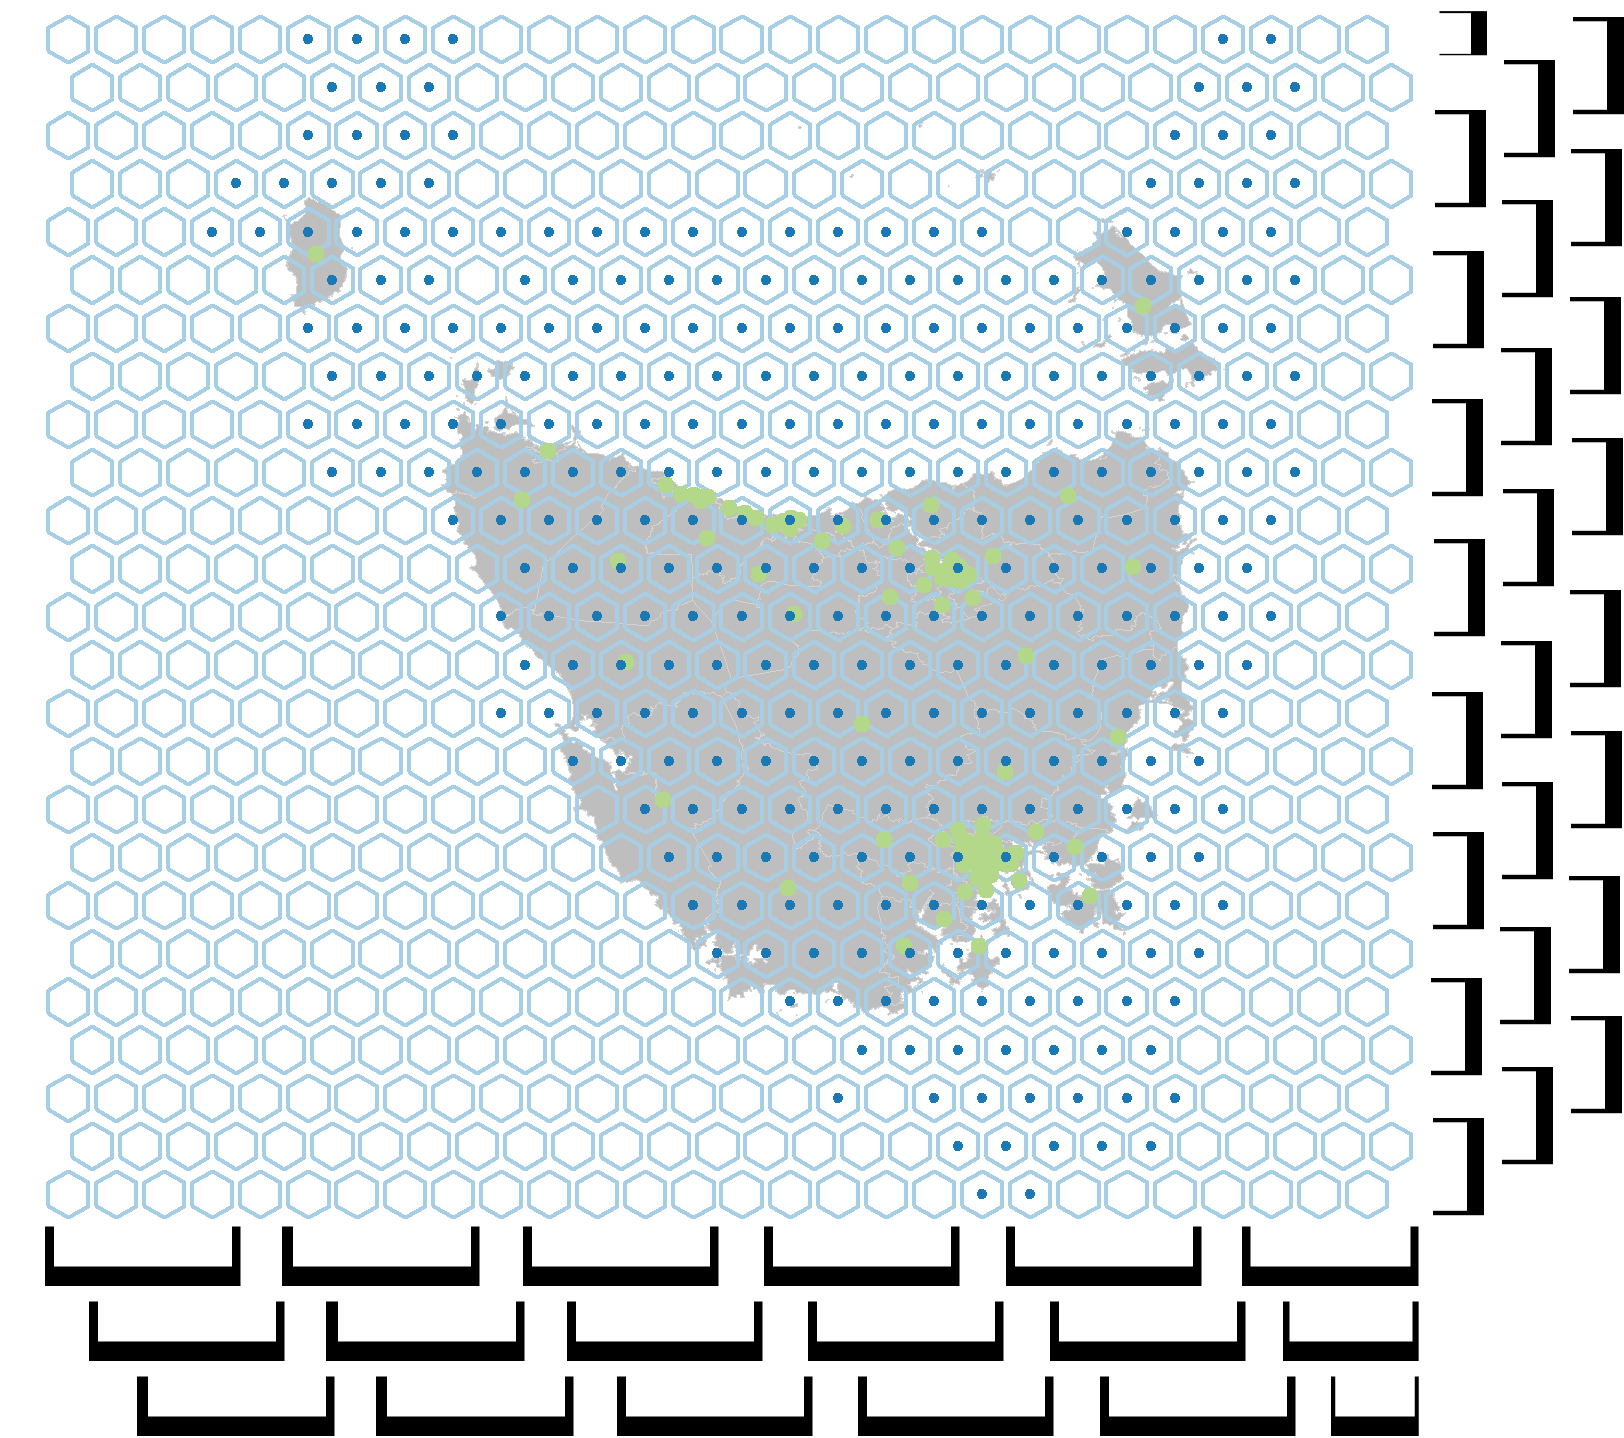
\includegraphics[width=16cm]{figures/03-algorithm/3grid.png}
\caption{\label{fig:filter-grid}All possible hexagon locations from the initial grid are shown with blue outlines. The blue dots show the grid points left to choose from after the buffer step. The rolling windows show the collections of rows and columns used to filter the hexagon locations.}
\end{figure}

\hypertarget{centroid-to-focal-point-distance}{%
\subsubsection{Centroid to focal point distance}\label{centroid-to-focal-point-distance}}

The distance between each centroid in the set, and each of the focal points provided is calculated. The name of the closest focal point, and the distance and angle from focal point to polygon centroid is joined to polygon data set. To minimise time taken for this step only one option is provided, Tasmania's capital city Hobart.
The order for allocation is determined by the distance between the polygon centroid and it's closest focal point. The points are arranged from the centroid closest to the focal point(s), to the furthest.

\hypertarget{allocate-each-centroid-to-a-hexagon-grid-point}{%
\subsubsection{Allocate each centroid to a hexagon grid point}\label{allocate-each-centroid-to-a-hexagon-grid-point}}

Allocation of all centroids takes place using the set of polygon centroids and the hexagon map grid.
Centroid allocation begins with the closest centroid to a focal point.
This will preserve spatial relationships with the focal point, as the inner city areas are allocated first, they will be placed closest to the capital, and the areas that are further will then be accommodated.
The possible hexagon grid points reduces by one after each allocation, then only those that have not yet been allocated are considered.

The possible hexagon locations to consider for a centroid are determined by the \texttt{hex\_filter}. This is the maximum amount of hexagons between the centroid and the furthest considered hexagon. It is used to subset possible grid points to only those surrounding the polygon centroid within an appropriate range. A smaller distance will increase speed, but can decrease accuracy when width of the angle increases.

\begin{Shaded}
\begin{Highlighting}[]
\NormalTok{hexmap_allocation <-}\StringTok{ }\KeywordTok{allocate}\NormalTok{(}
  \DataTypeTok{centroids =}\NormalTok{ centroids }\OperatorTok\StringTok{ }\KeywordTok{select}\NormalTok{(SA2_NAME16, longitude, latitude),}
  \DataTypeTok{sf_id =} \StringTok{"SA2_NAME16"}\NormalTok{,}
  \DataTypeTok{hex_grid =}\NormalTok{ grid,}
  \DataTypeTok{hex_size =} \FloatTok{0.2}\NormalTok{, }\CommentTok{## same size used in create_grid}
  \DataTypeTok{hex_filter =} \DecValTok{10}\NormalTok{,}
  \DataTypeTok{width =} \DecValTok{35}\NormalTok{,}
  \DataTypeTok{focal_points =}\NormalTok{ capital_cities,}
  \DataTypeTok{verbose =} \OtherTok{TRUE}\NormalTok{)}
\end{Highlighting}
\end{Shaded}

The following example considers the first of the Statistical Areas at Level 2.
Within the algorithm, these steps are repeated for each polygon.

\hypertarget{step-1-filter-the-grid-for-unassigned-hexagon-points}{%
\subparagraph{Step 1: Filter the grid for unassigned hexagon points}\label{step-1-filter-the-grid-for-unassigned-hexagon-points}}

Keeping only the available hexagon points prevents multiple geographic units from being allocated to the same hexagon.

\hypertarget{step-2-filter-the-grid-points-for-those-closest-to-the-centroid}{%
\subparagraph{Step 2: Filter the grid points for those closest to the centroid}\label{step-2-filter-the-grid-points-for-those-closest-to-the-centroid}}

A box of possible hexagon locations around the centroid allows only the closest points that are not yet assigned to be considered. The corners of the box may not appear square if the buffer step has already removed unnecessary points from over the ocean.

The algorithm then removes the outer corners of the square, creating a circle of points, by only keeping points within a certain radial distance around the original centroid location.

\begin{figure}[H]
\centering
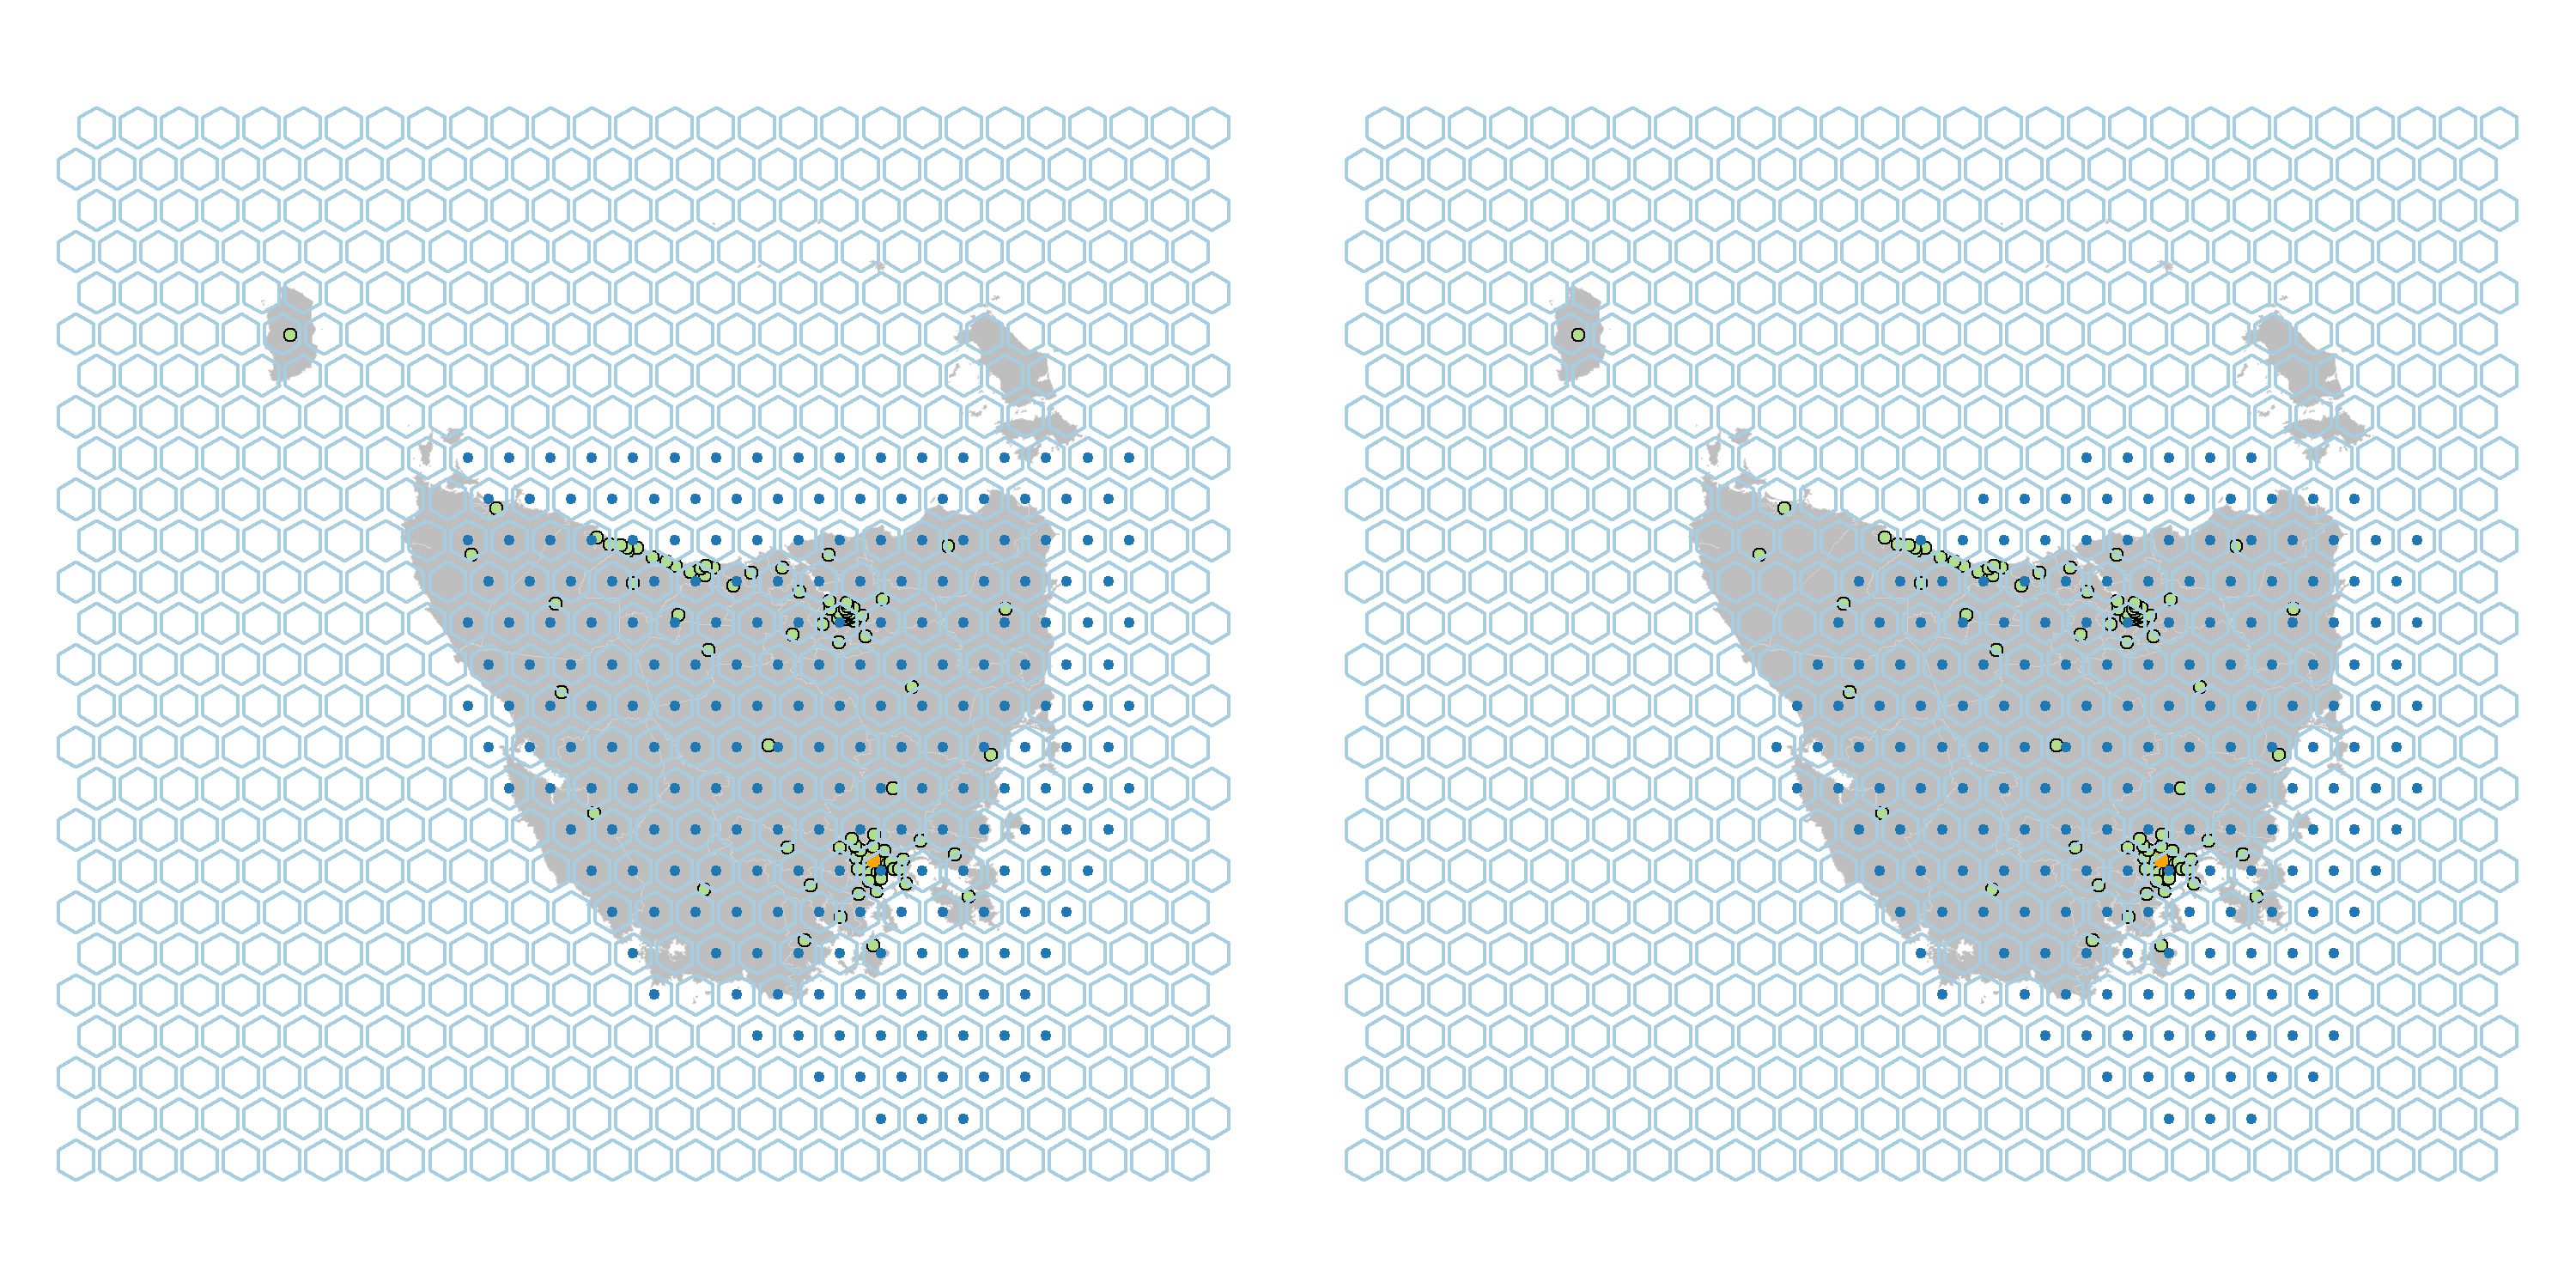
\includegraphics[width=16cm]{figures/03-algorithm/4grid.png}
\caption{\label{fig:buffers}Filter for grid points within a square, then circular, distance for those closest to the centroid.}
\end{figure}

The \texttt{width} parameter is used to take a slice of the remaining points. The width is the amount of degrees used on either side of the angle from the focal point to centroid location. This uses the angle from the closest capital city, to the current centroid as seen in Figure \ref{fig:angles} . This allows the spatial relationship to be preserved, even when it is allocated to a hexagon that is further from the focal point then the original centroid location.

\begin{figure}[H]
\centering
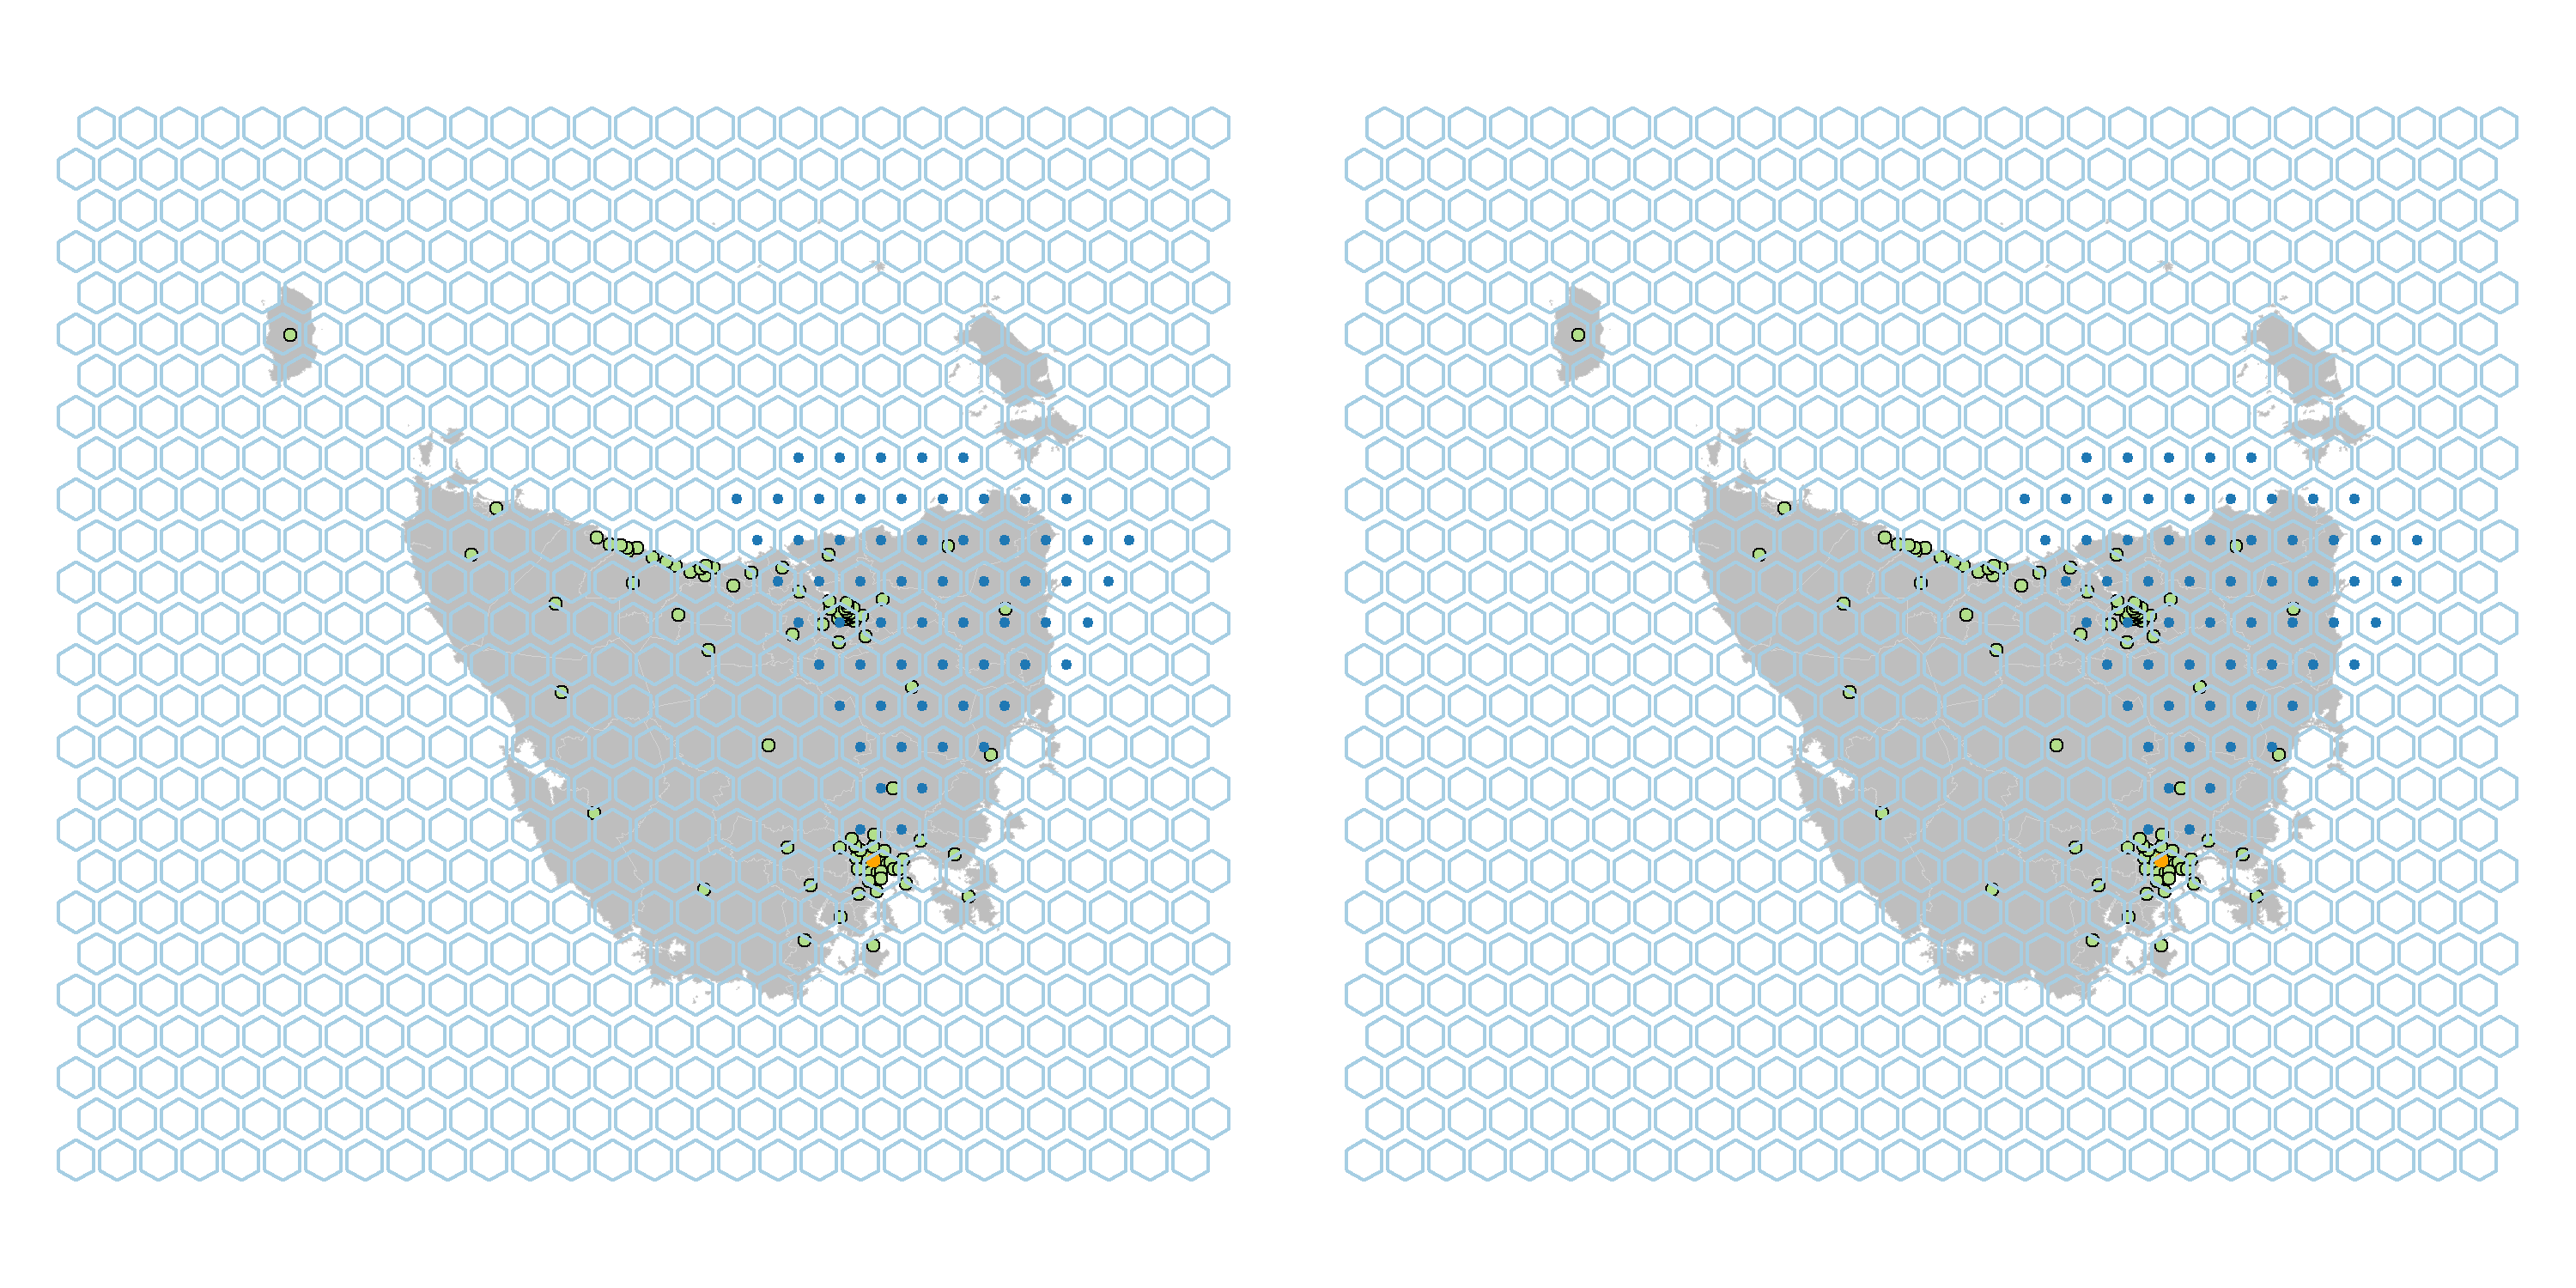
\includegraphics[width=16cm]{figures/03-algorithm/5allocate.png}
\caption{\label{fig:angles}Filter for grid points within the angle from the focal point to the centroid.}
\end{figure}

If no available hexagon grid point is found within the original filter distance and angle, the distance is expanded, only when a maximum distance is reached will the angle expand to accommodate more possible grid points.\\
By default the angle filter to hexagon grid points that fall within the bounds of the angle from the focal point to the geographic centroid, plus and minus 30 degrees. This will increase if no points can be found within the \texttt{hex\_filter} distance. The default angle of 30 was chosen to allow the algorithm to choose hexagons that best maintained the spatial relationship between the focal point and geographic centroid.

\begin{figure}[H]
\centering
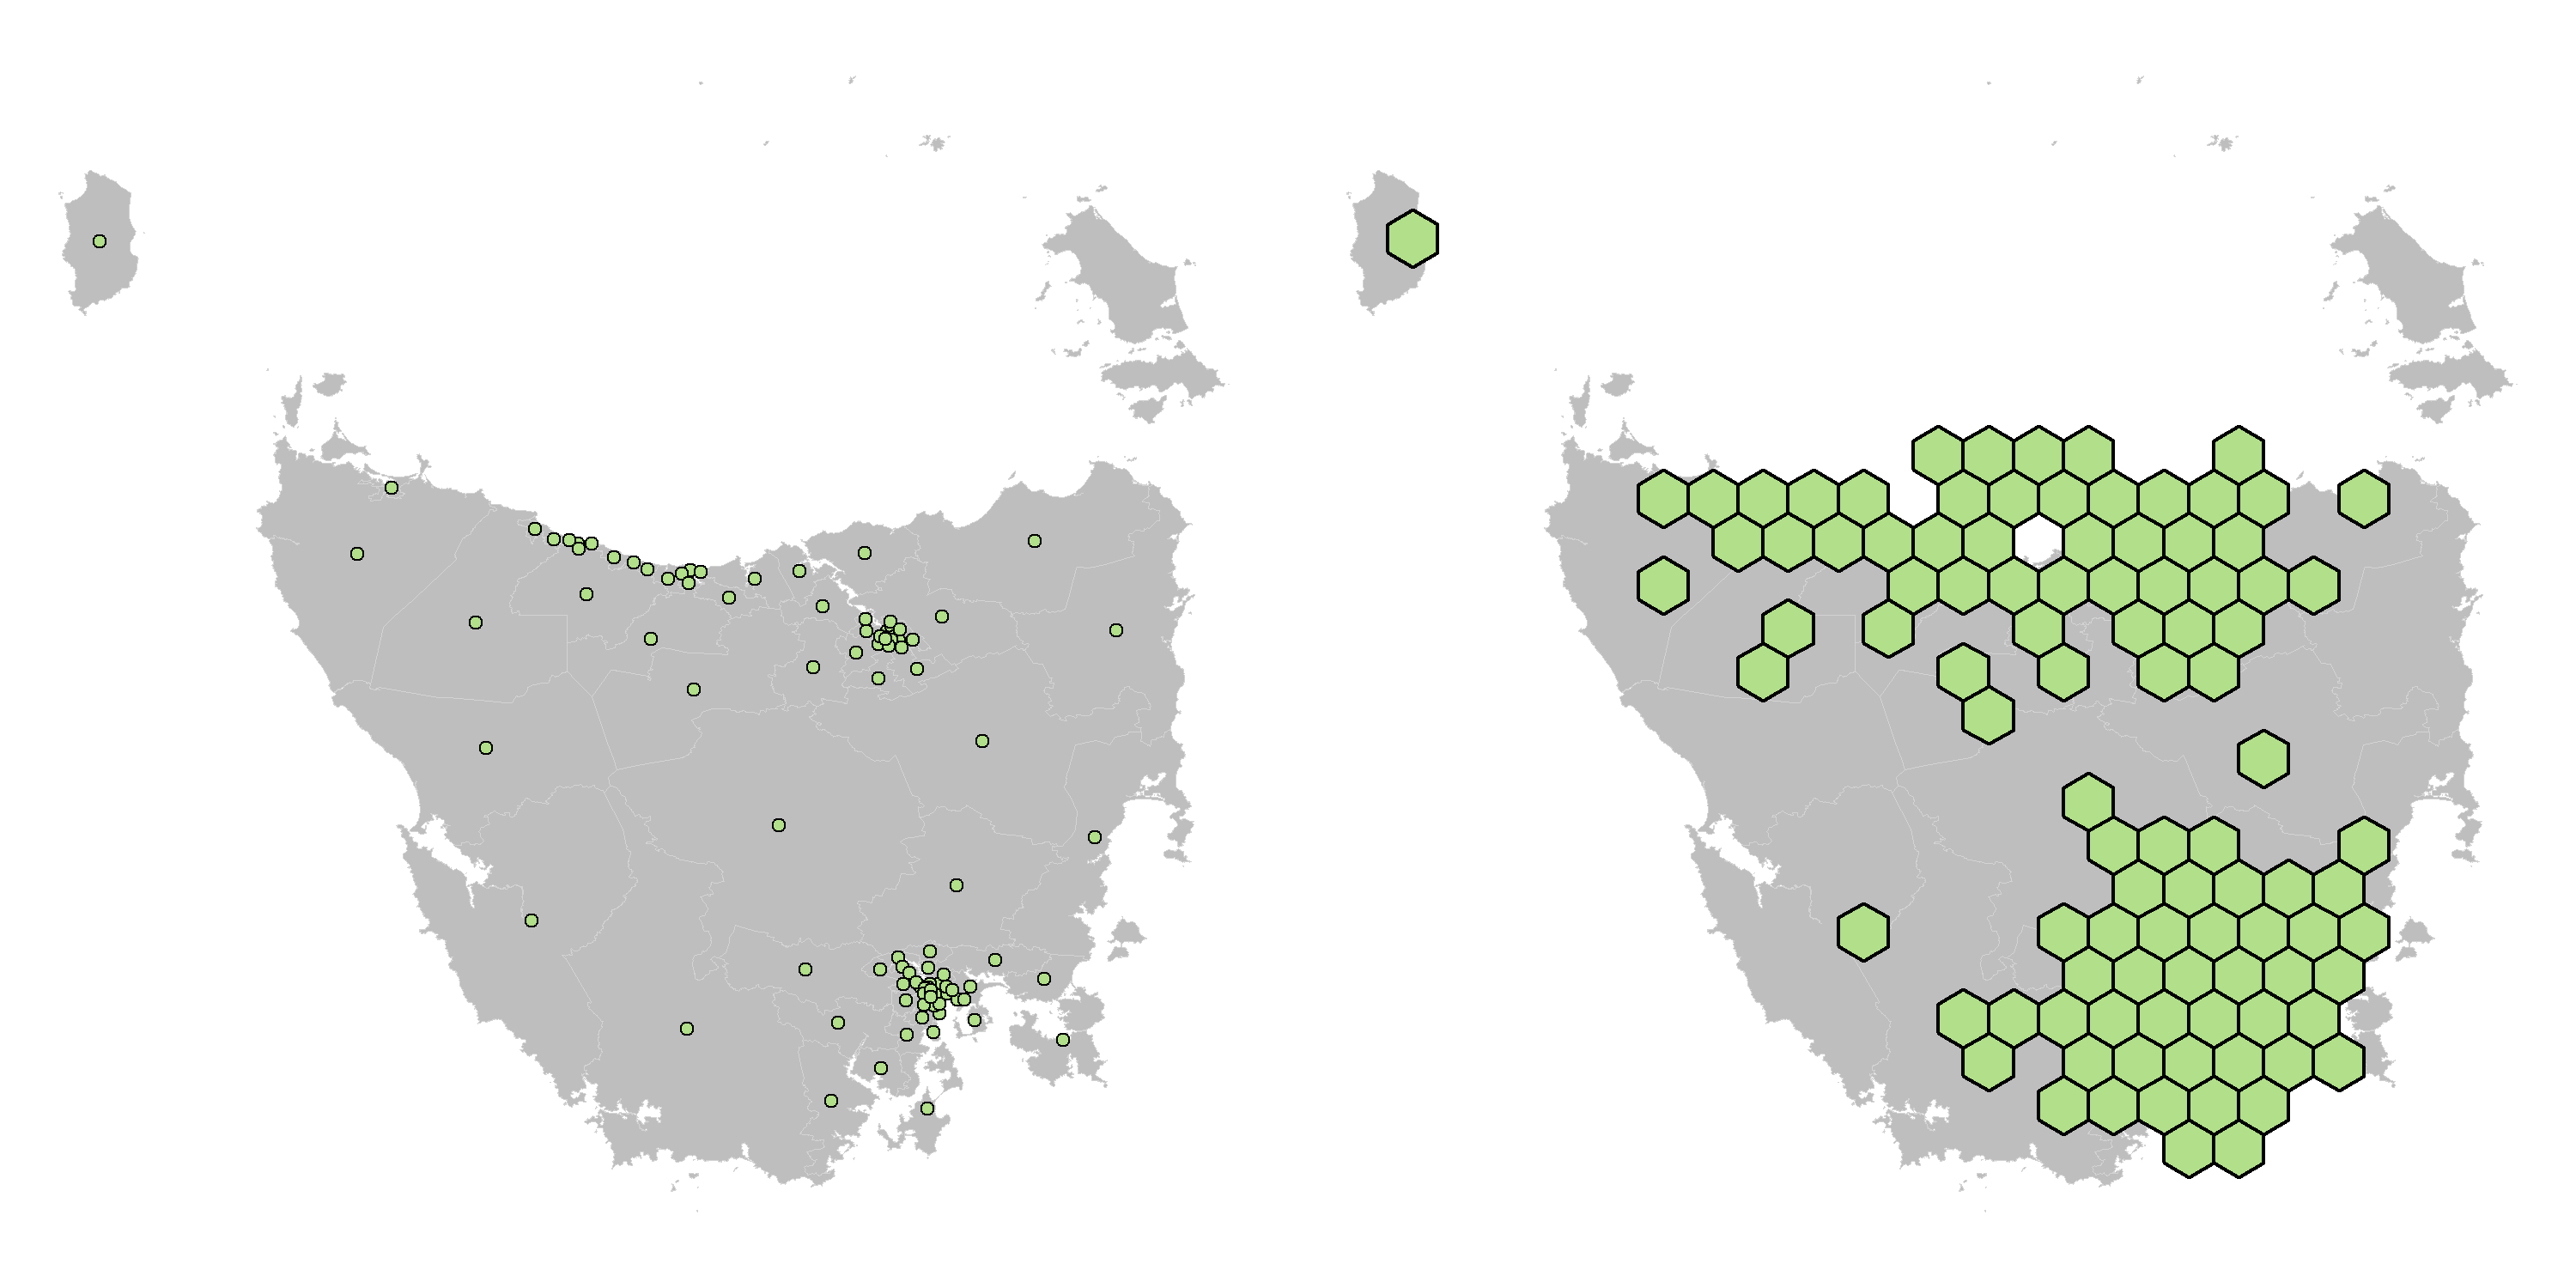
\includegraphics[width=16cm]{figures/03-algorithm/6allocate.png}
\caption{\label{fig:buffs}A complete hexagon tile map of Tasmania.}
\end{figure}

A complete hexagon tile map of Tasmania is created by applying the algorithm steps to each centroid.
The hexagon tile map visualisation is used below to visualise the Australian Cancer Atlas data. Two views of the same data are produced by filling according to the Lung Cancer Standardised Incidence Rates (SIRs) downloaded from the Australian Cancer Atlas site. This small example in Figure \ref{fig:sir} shows the group of blue areas in the Hobart CBD more prominently in the hexagon tile map (b).
The small red areas visible in the choropleth map (a) along the north coast are much larger in the hexagon tile maps. The hexagon tile map shows less yellow, this no longer overwhelms the map space with the information regarding the rural areas.

\begin{figure}[H]
\centering
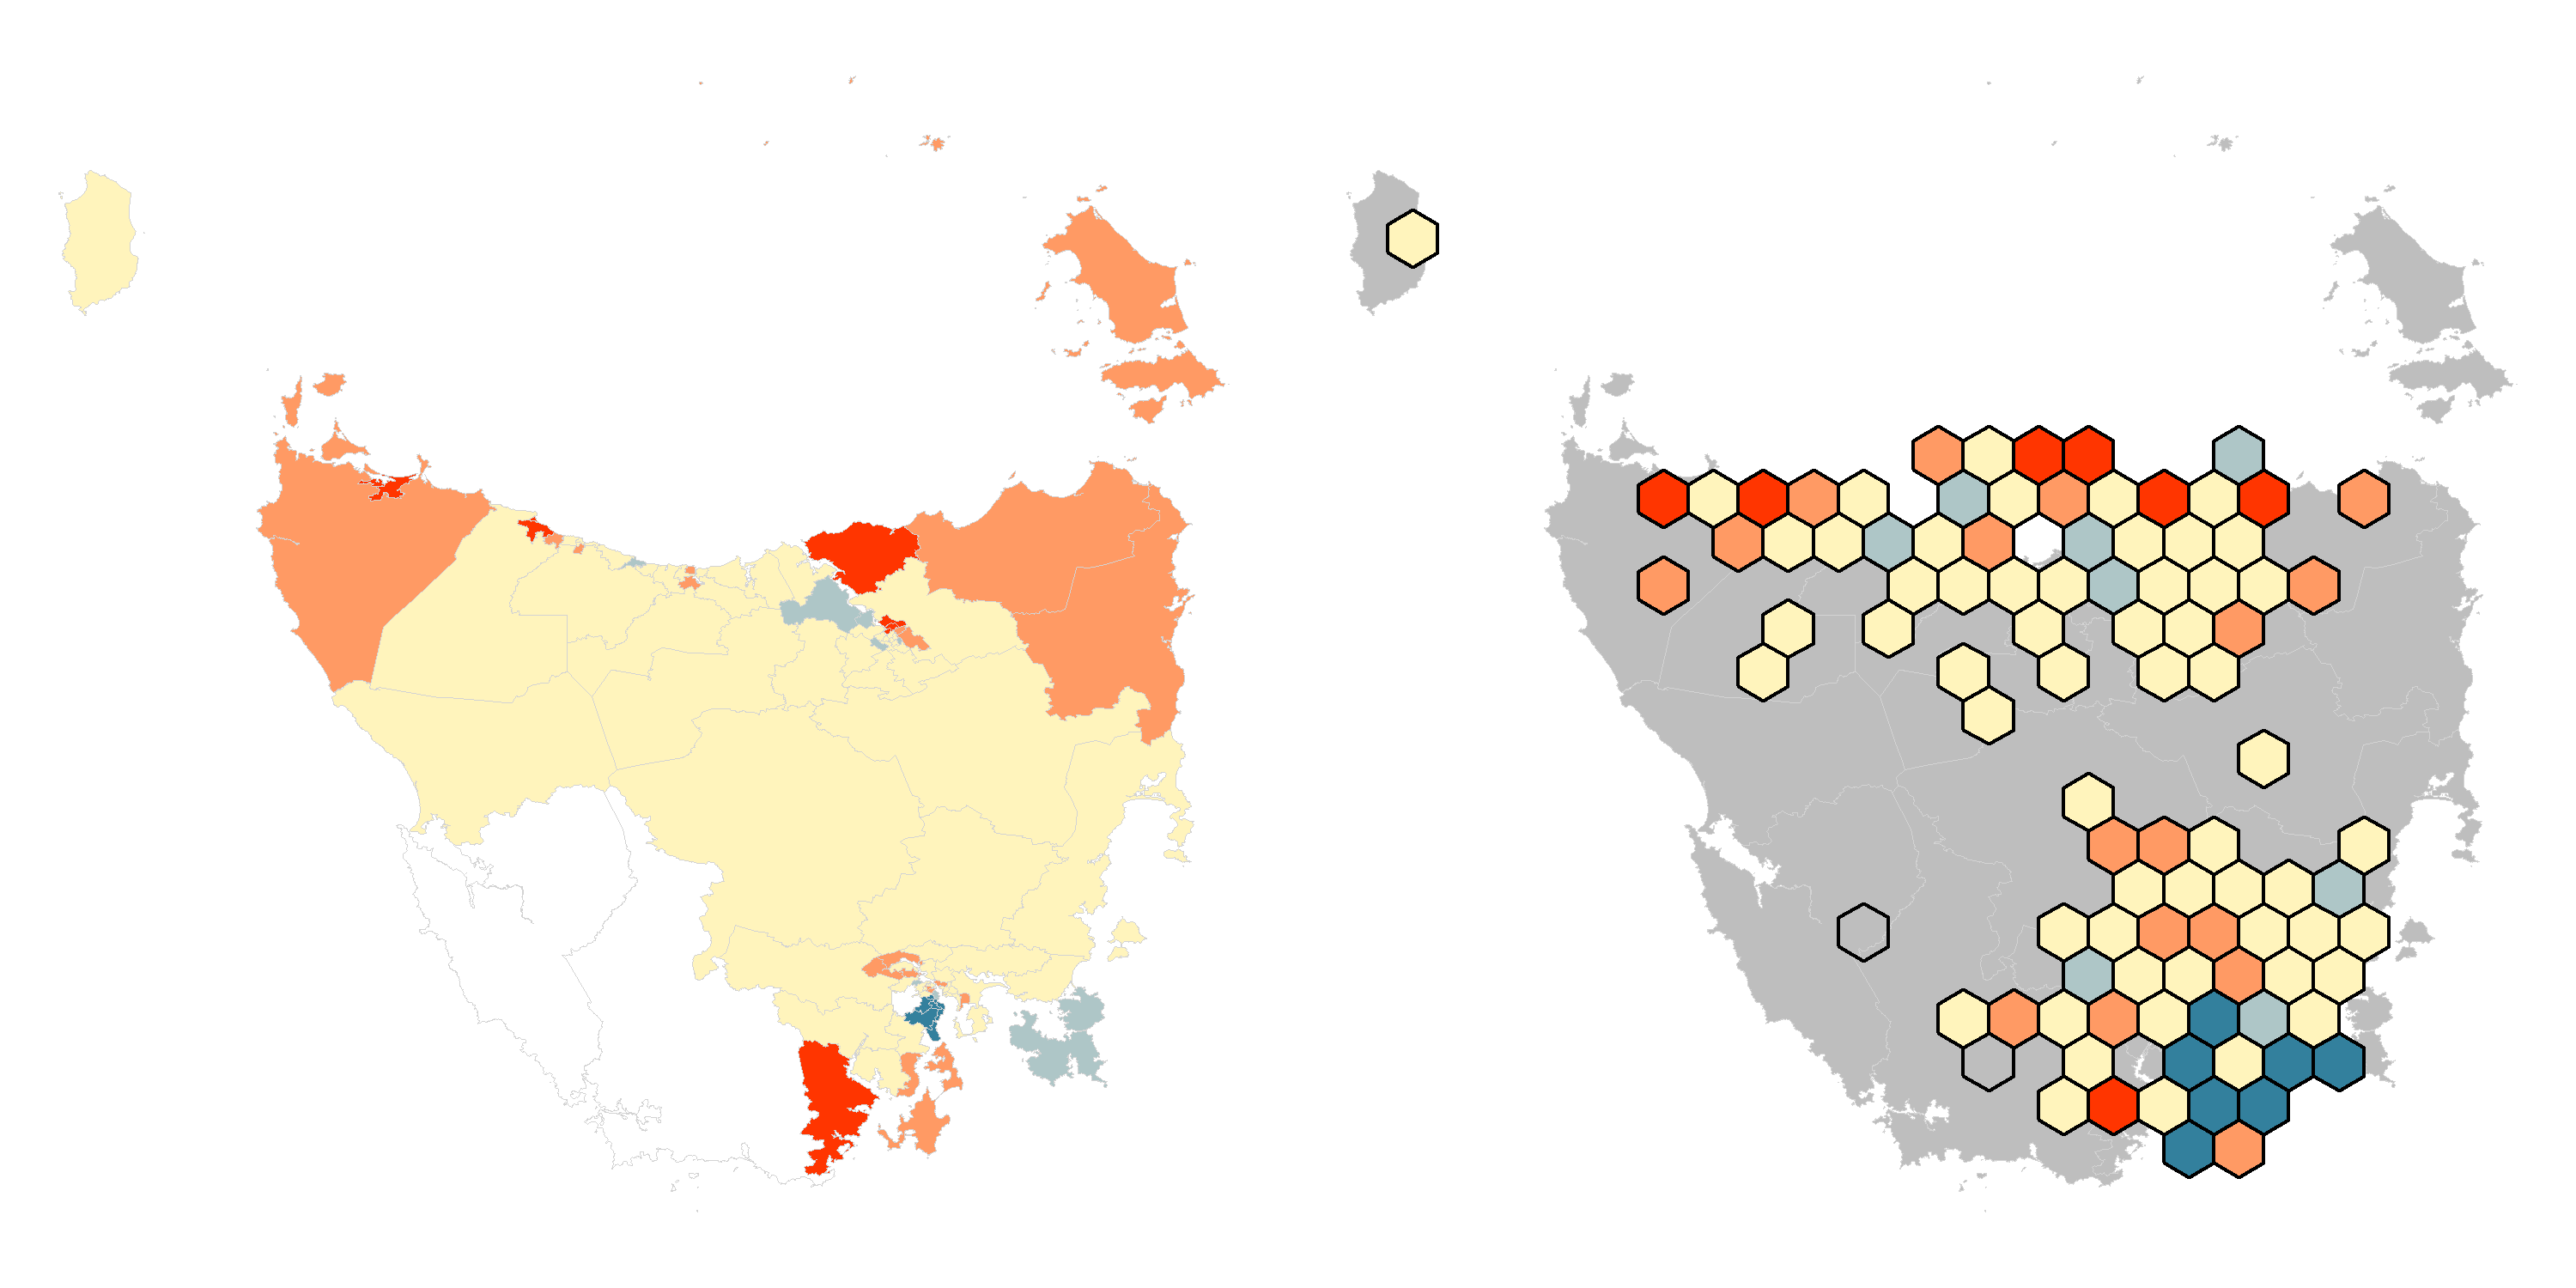
\includegraphics[width=16cm]{figures/03-algorithm/7SIR.png}
\caption{\label{fig:sir}The Australian Cancer Atlas data has determined the colour of each Statistical Area of Australian at Level 2. A choropleth map (a) of SIR is paired with a hexagon tile map (b) to contrast the colours that are made obvious when every SA2 is equally represented.}
\end{figure}

\hypertarget{neighbour-relationships}{%
\subsubsection{Neighbour relationships}\label{neighbour-relationships}}

It is possible to consider the neighbouring areas for each SA2, for stronger preservation of the spatial distribution.

An additional step can be included to allow the neighbours that have alredy been allocated to influence the placement of the current centroid.
This requires specifying the \texttt{sf} object as the argument for the \texttt{use\_neighbours} parameter. This calculates neighbours using intersections of their polygons. This occurs for all areas before any allocations begin.

During the allocation of each centroid, the list of neighbours is consulted. If any neighbour was already allocated, the hexagons surrounding the neighbours on the grid are prioritised. For multiple neighbours, the neighbouring hexagon grid points are aggregated and considered in order of distance from the original centroid.

\hypertarget{using-sugarbag}{%
\section{Using sugarbag}\label{using-sugarbag}}

\hypertarget{installation}{%
\subsubsection{Installation}\label{installation}}

The package can be installed from CRAN:

\begin{Shaded}
\begin{Highlighting}[]
\KeywordTok{install.packages}\NormalTok{(}\StringTok{"sugarbag"}\NormalTok{)}
\end{Highlighting}
\end{Shaded}

and the development version can be install from the GitHub repository:

\begin{Shaded}
\begin{Highlighting}[]
\NormalTok{devtools}\OperatorTok{::}\KeywordTok{install_github}\NormalTok{(}\StringTok{"srkobakian"}\NormalTok{,}\StringTok{"sugarbag"}\NormalTok{)}
\end{Highlighting}
\end{Shaded}

Load the library into your R session with:

\begin{Shaded}
\begin{Highlighting}[]
\KeywordTok{library}\NormalTok{(sugarbag)}
\end{Highlighting}
\end{Shaded}

\hypertarget{creating-a-hexagon-tile-map}{%
\subsubsection{Creating a hexagon tile map}\label{creating-a-hexagon-tile-map}}

The following code creates the hexagon tile map for all the Statistical Areas at Level 2 in Tasmania.

\begin{Shaded}
\begin{Highlighting}[]
\CommentTok{## Load data}
\KeywordTok{data}\NormalTok{(tas_sa2)}

\CommentTok{## Create centroids set}
\NormalTok{centroids <-}\StringTok{ }\KeywordTok{create_centroids}\NormalTok{(tas_sa2, }\StringTok{"SA2_NAME16"}\NormalTok{)}

\CommentTok{## Create hexagon grid}
\NormalTok{grid <-}\StringTok{ }\KeywordTok{create_grid}\NormalTok{(}\DataTypeTok{centroids =}\NormalTok{ centroids,}
    \DataTypeTok{hex_size =} \FloatTok{0.2}\NormalTok{,}
    \DataTypeTok{buffer_dist =} \FloatTok{1.2}\NormalTok{)}

\CommentTok{## Allocate polygon centroids to hexagon grid points}
\NormalTok{hex_allocated <-}\StringTok{ }\KeywordTok{allocate}\NormalTok{(}
  \DataTypeTok{centroids =}\NormalTok{ centroids,}
  \DataTypeTok{hex_grid =}\NormalTok{ grid,}
  \DataTypeTok{sf_id =} \StringTok{"SA2_NAME16"}\NormalTok{,}
  \CommentTok{## same column used in create_centroids}
  \DataTypeTok{hex_size =} \FloatTok{0.2}\NormalTok{,}
  \CommentTok{## same size used in create_grid}
  \DataTypeTok{hex_filter =} \DecValTok{10}\NormalTok{,}
  \DataTypeTok{use_neighbours =}\NormalTok{ tas_sa2,}
  \DataTypeTok{focal_points =}\NormalTok{ capital_cities }\OperatorTok\StringTok{ }\KeywordTok{filter}\NormalTok{(points }\OperatorTok{==}\StringTok{ "Hobart"}\NormalTok{),}
  \DataTypeTok{width =} \DecValTok{35}\NormalTok{,}
  \DataTypeTok{verbose =} \OtherTok{FALSE}\NormalTok{)}

\CommentTok{## Prepare to plot}
\NormalTok{fort_hex <-}\StringTok{ }\KeywordTok{fortify_hexagon}\NormalTok{(}\DataTypeTok{data =}\NormalTok{ hex_allocated,}
  \DataTypeTok{sf_id =} \StringTok{"SA2_NAME16"}\NormalTok{, }\DataTypeTok{hex_size =} \FloatTok{0.2}\NormalTok{)}

\CommentTok{## Make a plot}
\KeywordTok{library}\NormalTok{(ggplot2)}
\KeywordTok{ggplot}\NormalTok{(fort_hex) }\OperatorTok{+}\StringTok{ }
\StringTok{  }\KeywordTok{geom_polygon}\NormalTok{(}\KeywordTok{aes}\NormalTok{(}\DataTypeTok{x=}\NormalTok{long, }\DataTypeTok{y=}\NormalTok{lat, }\DataTypeTok{group=}\NormalTok{hex_id, }\DataTypeTok{fill =}\NormalTok{ lat)) }\OperatorTok{+}
\StringTok{  }\KeywordTok{scale_fill_distiller}\NormalTok{(}\StringTok{""}\NormalTok{, }\DataTypeTok{palette=}\StringTok{"PRGn"}\NormalTok{)}
\end{Highlighting}
\end{Shaded}

\hypertarget{applications}{%
\section{Applications}\label{applications}}

\hypertarget{australian-cancer-atlas}{%
\subsubsection{Australian Cancer Atlas}\label{australian-cancer-atlas}}

The Australian Cancer Atlas \autocite{TACA} allows estimates derived from the models of SIRs and excess deaths to be downloaded.
Figure \ref{fig:melanoma-geo} is a choropleth map that uses colour to display the estimated SIRs of melanoma cancer for all persons for each SA2. The Australian choropleth map display draws attention to the expanse of light blue areas across the rural communities in all states. The SA2s around Brisbane stand out as more orange and red.
Comparatively, the hexagon tile map display in Figure \ref{fig:melanoma-hex} draws attention to contrast of the blue areas in Sydney and Melbourne and the capital city of Brisbane. In both Sydney and Melbourne, the hexagons that represent the SA2 areas in the inner-city areas have lower than average Incidence Rates.

With careful consideration of the choropleth map, the small geographic inner city areas may have been noticed by viewers, but the hexagon tile map display emphasises them. The communities in northern Queensland and the Northern territory do not draw attention because of their size as in the choropleth, but their colour is still noticably below average when contrasted with the heaxgons further south.

To create this choropleth map the SA2 polygons for 2011 from the ABS. The SIRs for each geographic unit are joined to the appropriate polygons.

\begin{figure}[H]
\centering
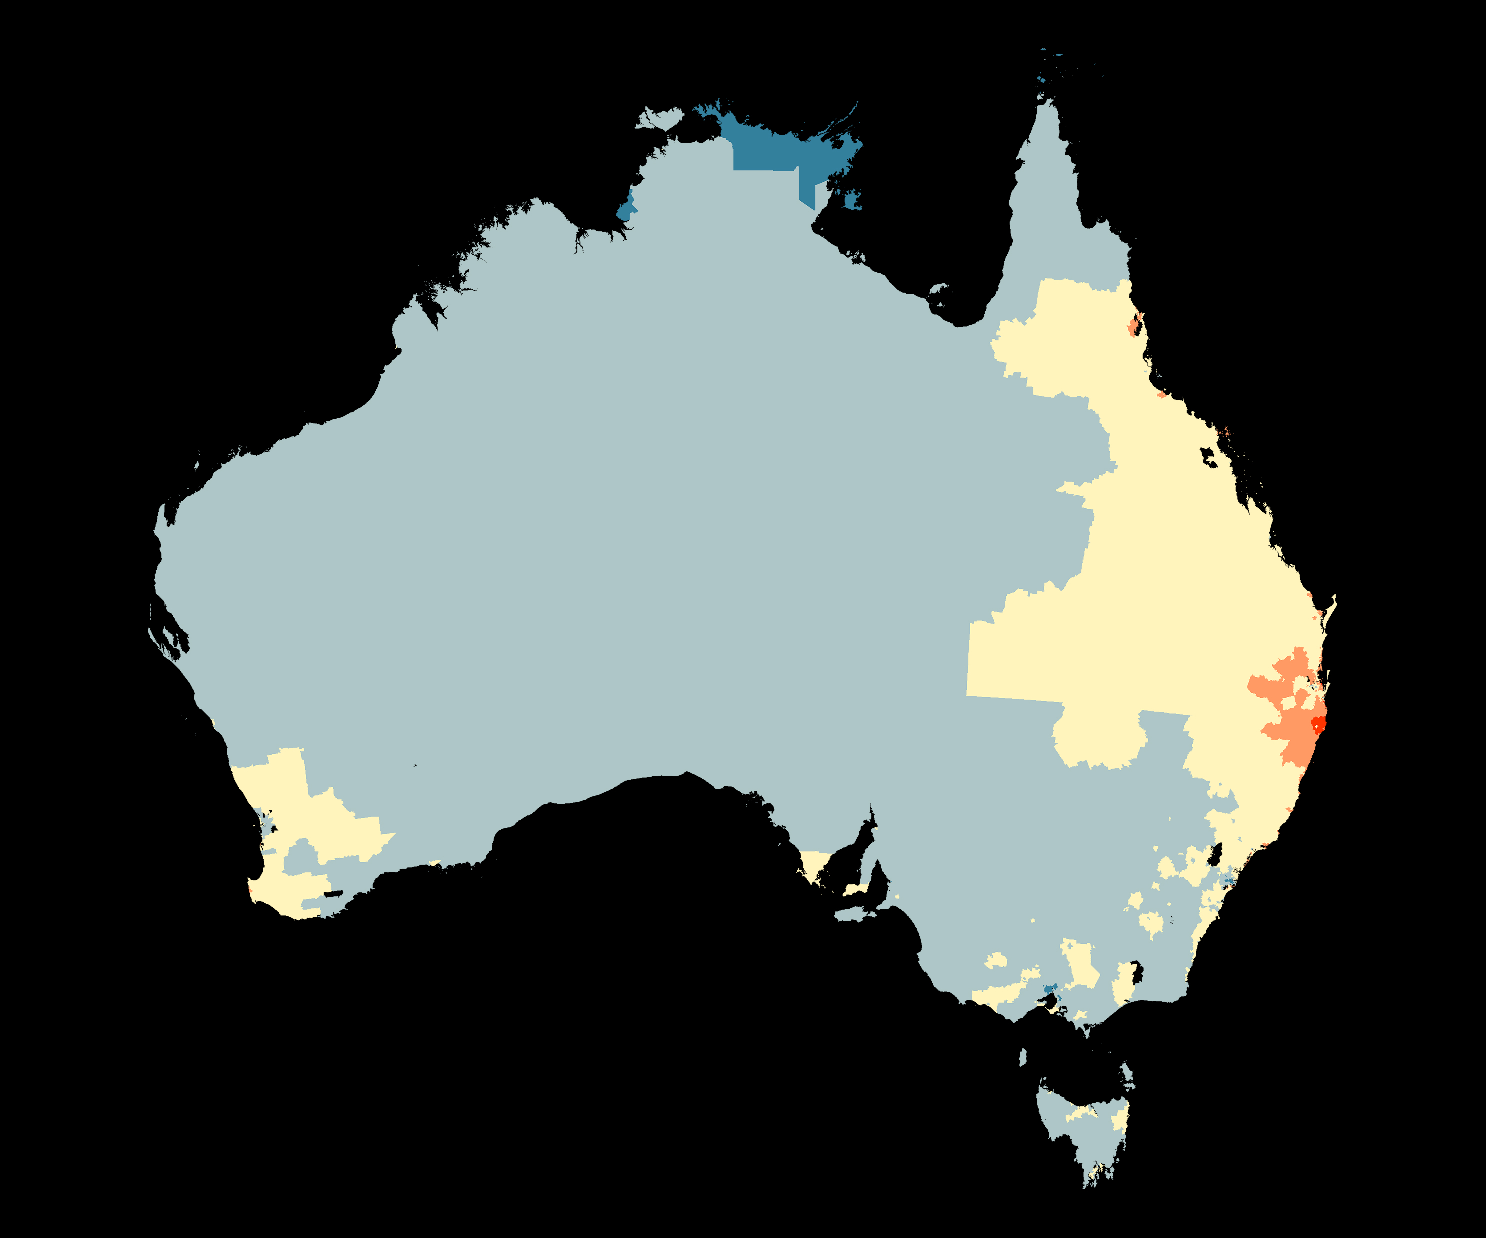
\includegraphics[width=16cm]{figures/03-algorithm/aus_melanoma_p.pdf}
\caption{\label{fig:melanoma-geo}A choropleth map of the Statistical Areas of Australia at Level 2. The colours communicate the value of the estimated SIR of Melanoma for all persons, they range from much lower than average (blue) to much higher than average (red)}
\end{figure}

To create the hexagon tile map display, the same steps are followed as outlined above:

\begin{itemize}
\tightlist
\item
  Create the set of centroid points
\item
  Create the hexagon grid points
\item
  Allocate each centroid to a hexagon grid point
\end{itemize}

\begin{figure}[H]
\centering
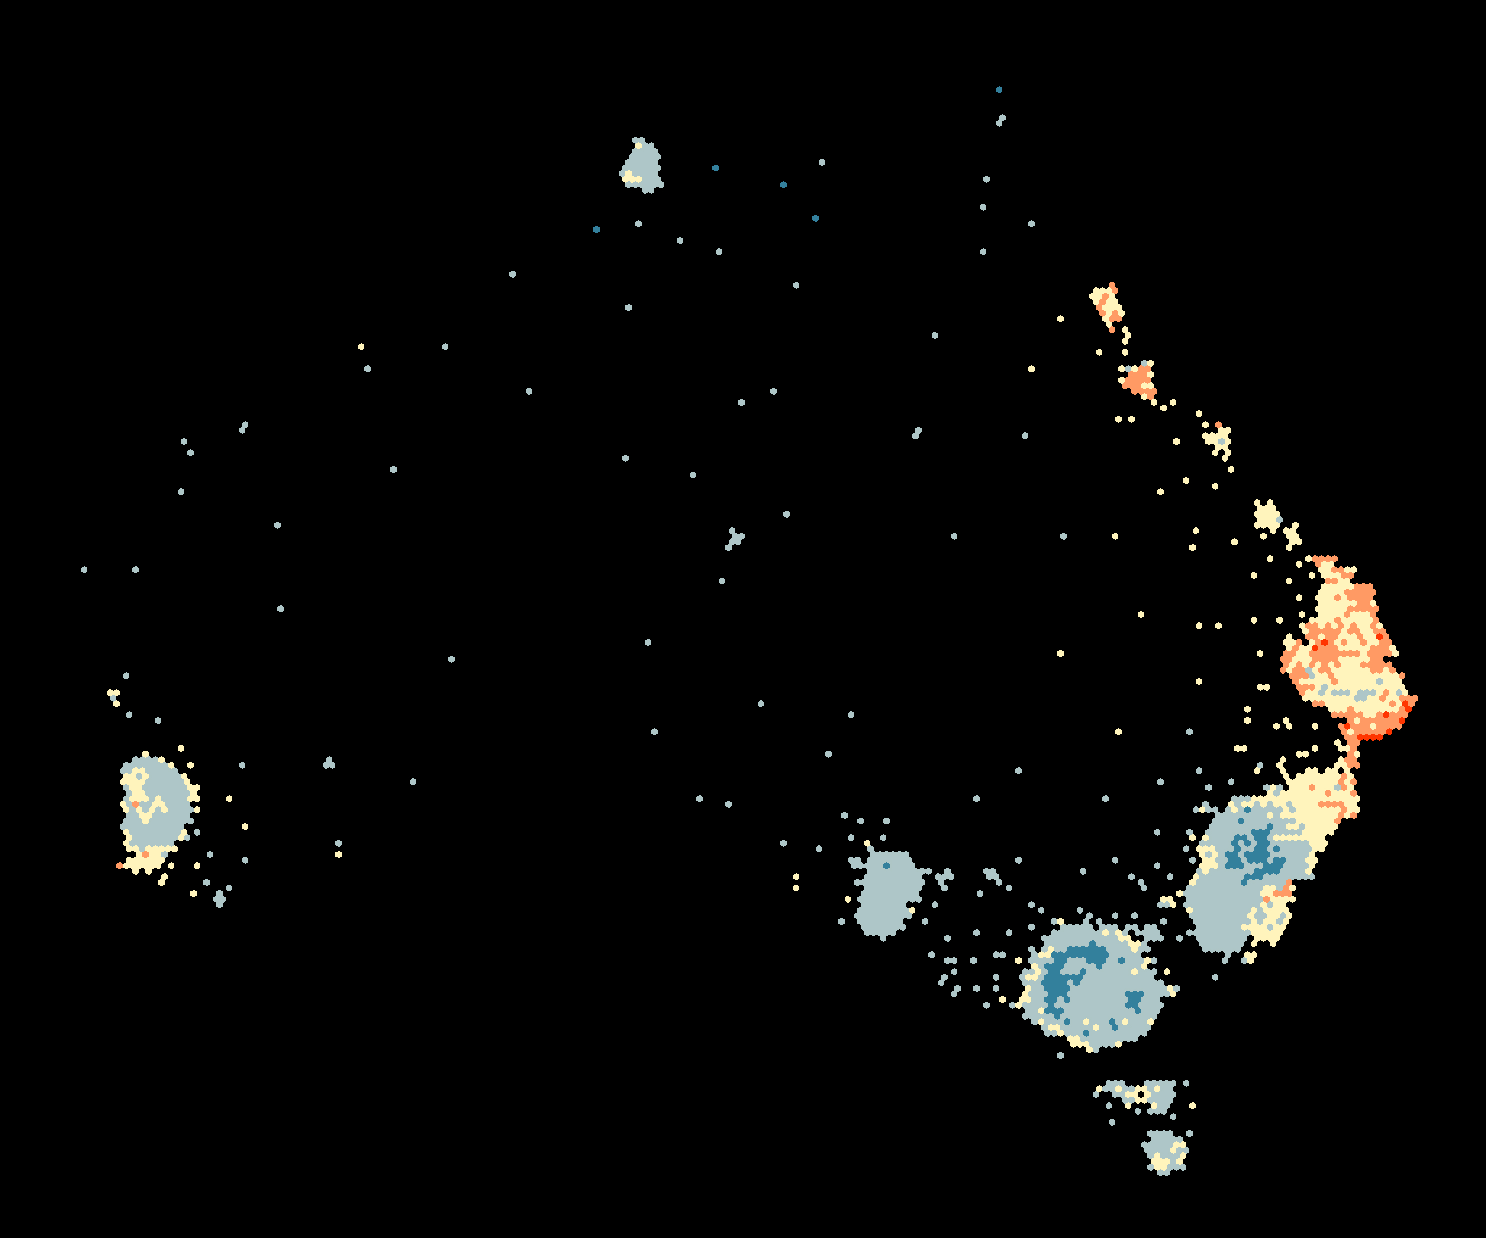
\includegraphics[width=16cm]{figures/03-algorithm/aus_melanoma_p_hex.pdf}
\caption{\label{fig:melanoma-hex}A hexagon tile map of the Statistical Areas of Australia at Level 2. The colours communicate the value of the estimated SIR, they range from much lower than average (blue) to much higher than average (red)}
\end{figure}

\hypertarget{animation}{%
\section{Animation}\label{animation}}

The \texttt{gganimate} \autocite{gganimate} package can be used to make an animation.
It requires connecting the polygons for each area in two displays, which can be done using the \texttt{sf\_id} variable, such as the SA2 name.
The animation\footnote{This animation can be viewed at: \url{https://sugarbagjss.netlify.com/}} connecting these two displays will highlight the rapid growth of the inner-city areas, and will decrease the large rural areas. The hexagons that move the furthest will move rapidly in the animation.

\hypertarget{conclusion}{%
\section{Conclusion}\label{conclusion}}

It is possible to use alternative maps to communicate spatial distributions.While a choropleth map display is the current practice spatial visualisation of geographical data. Current methods do not always work for Australia due to the large geographic space between the densely populated capital cities. The administrative boundaries may also distract from the statistics communicated using colour.

Alternative maps highlight the value of the statistics across the geographic units. Alternative mapping methods allow increased understanding of the spatial distribution of a variable across the population, by fairly representing each administrative area. This acknowledges that the amount of residents can be different but recognises that each population area is equally important. The solution to this visualisation problem has equally sized areas, with neighbourhood boundary connections. This map algorithm is implemented in the \texttt{sugarbag} \autocite{sugarbag} package written for \texttt{R} \autocite{R}.
The \texttt{sugarbag} package creates tesselated hexagon tile maps. The Australian application preserves the spatial relationships, emphasising capital cities. The hexagon tile map is a visualisation solution that highlights spatial distributions.

These hexagons equally represent each area. However, the tesselation does not allow the size of the hexagons to represent another variable, similar to the choropleth maps.
The algorithm is heavily dependent on the focal points used, as this determines the order of allocation. It works on the assumption that viewers can use directional relationships to identify their neighbourhoods but this can be aided by the animation.

Future work will include refining the algorithm. It would be possible to take a logarithmic function rather than a direct angle to help choose a closer hexagon to the original centroid location, before increasing the width of the angle used to filter the hexagons.

This algorithm has only been tested using single countries, and does not consider definite borders of countries. While the buffer allows extention beyond the furthest centroids, there is no mechanism to protect the borders and ensure centroids are placed within the geographic borders of a country.

This algorithm is an effective start to creating hexagon tile maps for many geographic units.

\hypertarget{ch:experiment}{%
\chapter{Comparing the Effectiveness of the Choropleth Map with a Hexagon Tile Map for Communicating Cancer}\label{ch:experiment}}

This chapter tests the performance of the hexagon tile map display created using the algorithm discussed in Section \ref{ch:algorithm}.
It outlines the lineup protocol method of visual inference that can be used to test the effectiveness of information visualisations.
Using a two factor experimental design, the experiment contrasts the performance of participants when they viewed a choropleth map, and their performance when viewing a hexagon tile map.
The experiment also considered three types of spatial trends, one geographic trend, and two population related distributions.
The results showed that participants did in fact more frequently find the population related distributions when using the hexagon tile map.

This chapter has been submitted to the journal \emph{IEEE Transactions of Visualisation and Computer Graphics}.

\includepdf[pages = {1-}, scale=0.8]{statement-of-contribution_experiment.pdf}

\hypertarget{abstract-3}{%
\section*{Abstract}\label{abstract-3}}
\addcontentsline{toc}{section}{Abstract}

The choropleth map display is commonly used for communicating spatial distributions across geographic areas. However, when choropleths are used the size of the geographic units will influence the understanding of the distribution derived by map users. The hexagon tile map is presented as an alternative display for visualizing population related distributions effectively. Visual inference is used to measure the power of the hexagon tile map design, and the choropleth is used as a comparison. The hexagon tile map display is tested using a distribution that is directly related to the geography, with values monotonically increasing from the North-West to South-East areas of Australia. This study finds in a hexagon tile map lineup the single map that contains a population related distribution is detected with greater probability than the same data displayed in a choropleth map. These findings should encourage map creators to implement alternative displays and consider a hexagon tile map when presenting spatial distributions of heterogeneous areas.

\begin{Shaded}
\begin{Highlighting}[]
\CommentTok{# Load Libraries}
\KeywordTok{library}\NormalTok{(tidyverse)}
\KeywordTok{library}\NormalTok{(readxl)}
\KeywordTok{library}\NormalTok{(broom)}
\KeywordTok{library}\NormalTok{(cowplot)}
\KeywordTok{library}\NormalTok{(png)}
\KeywordTok{library}\NormalTok{(grid)}
\KeywordTok{library}\NormalTok{(lme4)}
\KeywordTok{library}\NormalTok{(ggthemes)}
\KeywordTok{library}\NormalTok{(RColorBrewer)}
\KeywordTok{library}\NormalTok{(knitr)}
\KeywordTok{library}\NormalTok{(kableExtra)}

\KeywordTok{options}\NormalTok{(}\DataTypeTok{knitr.kable.digits =} \StringTok{"2"}\NormalTok{)}
\end{Highlighting}
\end{Shaded}

\begin{Shaded}
\begin{Highlighting}[]
\NormalTok{trend_colors <-}\StringTok{ }\KeywordTok{c}\NormalTok{(}
  \StringTok{"NW-SE"}\NormalTok{ =}\StringTok{ "#B2DF8A"}\NormalTok{,}
  \StringTok{"Three Cities"}\NormalTok{ =}\StringTok{ "#A6CEE3"}\NormalTok{,}
  \StringTok{"All Cities"}\NormalTok{ =}\StringTok{ "#1F78B4"}\NormalTok{)}
  
\NormalTok{type_colors <-}\StringTok{ }\KeywordTok{c}\NormalTok{(}
  \StringTok{"Choro."}\NormalTok{ =}\StringTok{ "#fcae91"}\NormalTok{,}
  \StringTok{"Hex."}\NormalTok{ =}\StringTok{ "#a50f15"}\NormalTok{)}

\NormalTok{detect_f_colors <-}\StringTok{ }\KeywordTok{c}\NormalTok{(}
  \StringTok{"No"}\NormalTok{ =}\StringTok{ "#66C2A5"}\NormalTok{,}
  \StringTok{"Yes"}\NormalTok{ =}\StringTok{ "#FC8D62"}\NormalTok{)}

\NormalTok{detect_colors <-}\StringTok{ }\KeywordTok{c}\NormalTok{(}
  \StringTok{"Detected? No"}\NormalTok{ =}\StringTok{ "#66C2A5"}\NormalTok{,}
  \StringTok{"Detected? Yes"}\NormalTok{ =}\StringTok{ "#FC8D62"}\NormalTok{)}

  \CommentTok{# Downloaded data}
\NormalTok{d <-}\StringTok{ }\KeywordTok{read_xlsx}\NormalTok{(}\StringTok{"data/experiment-export.xlsx"}\NormalTok{, }\DataTypeTok{sheet=}\DecValTok{2}\NormalTok{) }\OperatorTok
\StringTok{  }\KeywordTok{filter}\NormalTok{(}\OperatorTok{!}\KeywordTok{is.na}\NormalTok{(contributor)) }\OperatorTok
\StringTok{  }\KeywordTok{mutate}\NormalTok{(}\DataTypeTok{contributor =} \KeywordTok{factor}\NormalTok{(contributor))}

\CommentTok{# Check data set }
\CommentTok{# Need to clean multiple entries, 48, 24}
\CommentTok{# remove duplicated entries due to submit button}
\NormalTok{d <-}\StringTok{ }\NormalTok{d }\OperatorTok\StringTok{ }\KeywordTok{group_by}\NormalTok{(group, contributor, image_name) }\OperatorTok
\StringTok{  }\KeywordTok{slice}\NormalTok{(}\DecValTok{1}\NormalTok{) }\OperatorTok\StringTok{ }\KeywordTok{ungroup}\NormalTok{() }\OperatorTok\StringTok{ }
\StringTok{  }\KeywordTok{arrange}\NormalTok{(group, contributor, plot_order)}

\CommentTok{# Remove contributors who did not provide answers to most questions}
\NormalTok{keep <-}\StringTok{ }\NormalTok{d }\OperatorTok\StringTok{ }\KeywordTok{count}\NormalTok{(contributor, }\DataTypeTok{sort =} \OtherTok{TRUE}\NormalTok{) }\OperatorTok\StringTok{ }\KeywordTok{filter}\NormalTok{(n }\OperatorTok{>}\StringTok{ }\DecValTok{10}\NormalTok{)}
\NormalTok{d <-}\StringTok{ }\NormalTok{d }\OperatorTok\StringTok{ }
\StringTok{  }\KeywordTok{filter}\NormalTok{(contributor }\OperatorTok\StringTok{ }\NormalTok{keep}\OperatorTok{$}\NormalTok{contributor) }\OperatorTok
\StringTok{  }\KeywordTok{filter}\NormalTok{(contributor }\OperatorTok{!=}\StringTok{ "1234567890"}\NormalTok{)}

\CommentTok{# Remove contributors who did not provide any choices}
\CommentTok{# Or an insufficient amount of responses}
\NormalTok{bad_contribs <-}\StringTok{ }\NormalTok{d }\OperatorTok\StringTok{ }\KeywordTok{group_by}\NormalTok{(contributor) }\OperatorTok\StringTok{ }
\StringTok{  }\KeywordTok{summarise}\NormalTok{(}\DataTypeTok{sum0 =} \KeywordTok{sum}\NormalTok{(choice)) }\OperatorTok\StringTok{ }
\StringTok{  }\KeywordTok{filter}\NormalTok{(sum0 }\OperatorTok{<}\StringTok{ }\DecValTok{13}\NormalTok{) }\OperatorTok\StringTok{ }
\StringTok{  }\KeywordTok{pull}\NormalTok{(contributor)}

\NormalTok{d <-}\StringTok{ }\NormalTok{d }\OperatorTok\StringTok{ }
\StringTok{  }\KeywordTok{filter}\NormalTok{(}\OperatorTok{!}\NormalTok{(contributor }\OperatorTok\StringTok{ }\NormalTok{bad_contribs))}


\NormalTok{n_contributors <-}\StringTok{ }\NormalTok{d }\OperatorTok\StringTok{ }\KeywordTok{count}\NormalTok{(contributor, }\DataTypeTok{sort=}\OtherTok{TRUE}\NormalTok{) }\OperatorTok\StringTok{ }
\StringTok{  }\KeywordTok{summarise}\NormalTok{(}\DataTypeTok{n_contributors =} \KeywordTok{length}\NormalTok{(contributor))}

\NormalTok{d <-}\StringTok{ }\NormalTok{d }\OperatorTok\StringTok{ }\KeywordTok{mutate}\NormalTok{(}\DataTypeTok{certainty =} \KeywordTok{factor}\NormalTok{(}\KeywordTok{as.character}\NormalTok{(certainty),}
  \DataTypeTok{levels =} \KeywordTok{c}\NormalTok{(}\StringTok{"1"}\NormalTok{, }\StringTok{"2"}\NormalTok{, }\StringTok{"3"}\NormalTok{, }\StringTok{"4"}\NormalTok{,}\StringTok{"5"}\NormalTok{), }\DataTypeTok{ordered=}\OtherTok{TRUE}\NormalTok{))}
\end{Highlighting}
\end{Shaded}

\begin{Shaded}
\begin{Highlighting}[]
\NormalTok{replicate <-}\StringTok{ }\KeywordTok{tibble}\NormalTok{(}\DataTypeTok{image_name =} \KeywordTok{c}\NormalTok{(}\StringTok{"aus_cities_12_geo.png"}\NormalTok{, }\StringTok{"aus_cities_12_hex.png"}\NormalTok{, }
                                   \StringTok{"aus_cities_3_geo.png"}\NormalTok{, }\StringTok{"aus_cities_3_hex.png"}\NormalTok{,}
                                   \StringTok{"aus_cities_4_geo.png"}\NormalTok{, }\StringTok{"aus_cities_4_hex.png"}\NormalTok{,}
                                   \StringTok{"aus_cities_9_geo.png"}\NormalTok{, }\StringTok{"aus_cities_9_hex.png"}\NormalTok{,}
                                   \StringTok{"aus_nwse_2_geo.png"}\NormalTok{, }\StringTok{"aus_nwse_2_hex.png"}\NormalTok{,}
                                   \StringTok{"aus_nwse_3_geo.png"}\NormalTok{, }\StringTok{"aus_nwse_3_hex.png"}\NormalTok{,}
                                   \StringTok{"aus_nwse_5_geo.png"}\NormalTok{, }\StringTok{"aus_nwse_5_hex.png"}\NormalTok{,}
                                   \StringTok{"aus_nwse_6_geo.png"}\NormalTok{, }\StringTok{"aus_nwse_6_hex.png"}\NormalTok{,}
                                   \StringTok{"aus_three_12_geo.png"}\NormalTok{, }\StringTok{"aus_three_12_hex.png"}\NormalTok{,}
                                   \StringTok{"aus_three_5_geo.png"}\NormalTok{, }\StringTok{"aus_three_5_hex.png"}\NormalTok{,}
                                   \StringTok{"aus_three_8_geo.png"}\NormalTok{, }\StringTok{"aus_three_8_hex.png"}\NormalTok{,}
                                   \StringTok{"aus_three_9_geo.png"}\NormalTok{, }\StringTok{"aus_three_9_hex.png"}\NormalTok{),}
                    \DataTypeTok{replicate =} \KeywordTok{c}\NormalTok{(}\DecValTok{1}\NormalTok{, }\DecValTok{1}\NormalTok{, }\DecValTok{2}\NormalTok{, }\DecValTok{2}\NormalTok{, }\DecValTok{3}\NormalTok{, }\DecValTok{3}\NormalTok{, }\DecValTok{4}\NormalTok{, }\DecValTok{4}\NormalTok{, }
                                  \DecValTok{1}\NormalTok{, }\DecValTok{1}\NormalTok{, }\DecValTok{2}\NormalTok{, }\DecValTok{2}\NormalTok{, }\DecValTok{3}\NormalTok{, }\DecValTok{3}\NormalTok{, }\DecValTok{4}\NormalTok{, }\DecValTok{4}\NormalTok{,}
                                  \DecValTok{1}\NormalTok{, }\DecValTok{1}\NormalTok{, }\DecValTok{2}\NormalTok{, }\DecValTok{2}\NormalTok{, }\DecValTok{3}\NormalTok{, }\DecValTok{3}\NormalTok{, }\DecValTok{4}\NormalTok{, }\DecValTok{4}\NormalTok{))}
\CommentTok{# Add rep info to data}
\NormalTok{d <-}\StringTok{ }\NormalTok{d }\OperatorTok\StringTok{ }\KeywordTok{left_join}\NormalTok{(., replicate, }\DataTypeTok{by =} \StringTok{"image_name"}\NormalTok{)}
\end{Highlighting}
\end{Shaded}

\begin{Shaded}
\begin{Highlighting}[]
\CommentTok{# Tidy for analysis}
\NormalTok{d <-}\StringTok{ }\NormalTok{d }\OperatorTok\StringTok{ }
\StringTok{  }\KeywordTok{separate}\NormalTok{(image_name, }\KeywordTok{c}\NormalTok{(}\StringTok{"nothing"}\NormalTok{, }\StringTok{"trend"}\NormalTok{, }\StringTok{"location"}\NormalTok{, }\StringTok{"type"}\NormalTok{, }\StringTok{"extra"}\NormalTok{), }\DataTypeTok{remove =} \OtherTok{FALSE}\NormalTok{) }\OperatorTok
\StringTok{  }\KeywordTok{select}\NormalTok{(}\OperatorTok{-}\NormalTok{nothing, }\OperatorTok{-}\NormalTok{extra) }\OperatorTok
\StringTok{  }\KeywordTok{mutate}\NormalTok{(}\DataTypeTok{location =} \KeywordTok{as.numeric}\NormalTok{(location), }
    \CommentTok{# detect measures the accuracy of the choice}
         \DataTypeTok{detect =} \KeywordTok{ifelse}\NormalTok{(location }\OperatorTok{==}\StringTok{ }\NormalTok{choice, }\DecValTok{1}\NormalTok{, }\DecValTok{0}\NormalTok{)) }\OperatorTok\StringTok{ }
\StringTok{  }\KeywordTok{mutate}\NormalTok{(}\DataTypeTok{trend =} \KeywordTok{case_when}\NormalTok{(}
\NormalTok{    trend }\OperatorTok{==}\StringTok{ "nwse"} \OperatorTok{~}\StringTok{ "NW-SE"}\NormalTok{,}
\NormalTok{    trend }\OperatorTok{==}\StringTok{ "cities"} \OperatorTok{~}\StringTok{ "All Cities"}\NormalTok{,}
\NormalTok{    trend }\OperatorTok{==}\StringTok{ "three"} \OperatorTok{~}\StringTok{ "Three Cities"}\NormalTok{)) }\OperatorTok\StringTok{ }
\StringTok{  }\KeywordTok{mutate}\NormalTok{(}\DataTypeTok{trend =} \KeywordTok{fct_relevel}\NormalTok{(trend, }\StringTok{"NW-SE"}\NormalTok{,}\StringTok{"Three Cities"}\NormalTok{,}\StringTok{"All Cities"}\NormalTok{)) }\OperatorTok\StringTok{ }
\StringTok{  }\KeywordTok{mutate}\NormalTok{(}\DataTypeTok{type =} \KeywordTok{case_when}\NormalTok{(}
\NormalTok{    type }\OperatorTok{==}\StringTok{ "hex"} \OperatorTok{~}\StringTok{"Hex."}\NormalTok{,}
    \OtherTok{TRUE}\OperatorTok{~}\StringTok{"Choro."}\NormalTok{)) }\OperatorTok\StringTok{ }
\StringTok{    }\KeywordTok{mutate}\NormalTok{(}\DataTypeTok{detect_f =} \KeywordTok{factor}\NormalTok{(detect, }\DataTypeTok{levels =} \KeywordTok{c}\NormalTok{(}\DecValTok{0}\NormalTok{,}\DecValTok{1}\NormalTok{), }\DataTypeTok{labels =} \KeywordTok{c}\NormalTok{(}\StringTok{"Detected? No"}\NormalTok{, }\StringTok{"Detected? Yes"}\NormalTok{)))}

\NormalTok{plots <-}\StringTok{ }\NormalTok{d }\OperatorTok\StringTok{ }\KeywordTok{group_by}\NormalTok{(group, trend, type, location) }\OperatorTok
\StringTok{  }\CommentTok{# pdetect measures the aggregated accuracy of the choices}
\StringTok{  }\KeywordTok{summarise}\NormalTok{(}\DataTypeTok{pdetect =} \KeywordTok{length}\NormalTok{(detect[detect }\OperatorTok{==}\StringTok{ }\DecValTok{1}\NormalTok{])}\OperatorTok{/}\KeywordTok{length}\NormalTok{(detect)) }
\end{Highlighting}
\end{Shaded}

\hypertarget{introduction-2}{%
\section{Introduction}\label{introduction-2}}

This study compares the effectiveness of the spatial display, a hexagon tile map, against the standard, a choropleth map, for communicating information about disease statistics. The choropleth map is the traditional method for visualizing aggregated statistics across administrative boundaries. The hexagon tile map builds on existing displays, such as the cartogram, and tessellated hexagon displays. A hexagon tile map forgoes the familiar boundaries, in favor of representing each geographic unit as an equally sized hexagon, placed approximately in the correct spatial location. It differs in the relaxed requirement to have connected hexagons, and allows sparsely located hexagons. This type of display may be useful for other countries, and other purposes. The algorithm to construct a hexagon tile map is available in the R package sugarbag \autocite{sugarbag}.

The hexagon tile map was designed for Australia, motivated by a need to display spatial statistics for the Australian Cancer Atlas. None of the existing approaches for creating cartograms or hexagon tiling perform well for the Australian landscape, which has vast open spaces and concentrations of population in small regions clustered on the coastlines.

The Australian Cancer Atlas {[}TACA{]} is an online interactive web tool created to explore the burden of cancer on Australian communities. There are many cancer types to be explored individually or aggregated. The Australian Cancer Atlas allows users to explore the patterns in the distributions of cancer statistics over the geographic space of Australia. It uses a choropleth map display and diverging color scheme to draw attention to relationships between neighboring areas. The hexagon tile map may be a useful alternative display to enhance the atlas.

The experiment was conducted using the lineup protocol, a visual inference procedure \autocite{GIIV}, to objectively test the effectiveness of the two displays.

The paper is organised as follows. The next section discusses the background of geographic data display and visual inference procedures. The \protect\hyperlink{methodology}{Methodology} section describes the methods for conducting the experiment and analysing the results. The results are summarized in the \protect\hyperlink{results}{Results} section.

\hypertarget{background}{%
\section{Background}\label{background}}

\hypertarget{spatial-data-displays}{%
\subsection{Spatial data displays}\label{spatial-data-displays}}

Spatial visualisations communicate the distribution of statistics over geographic landscapes. The choropleth map \autocite{EI}, \autocite{BCM} is a traditional display. It is used to present statistics that have been aggregated on geographic units. Creating a choropleth map involves drawing polygons representing the administrative boundaries, and filling with colour mapped to the value of the statistic. The choropleth map places the statistic in the context of the spatial domain, so that the reader can see whether there are spatial trends, clusters or anomalies. This is important for digesting disease patterns. If there is a trend it may imply that the disease is spreading from one location to another. If there is a cluster, or an anomaly, there may be a localized outbreak of the disease. Aggregating the statistic on administrative units, provides a level of privacy to individuals, while allowing the impact of the disease on the community to be analyzed.

\begin{figure}[H]
\centering
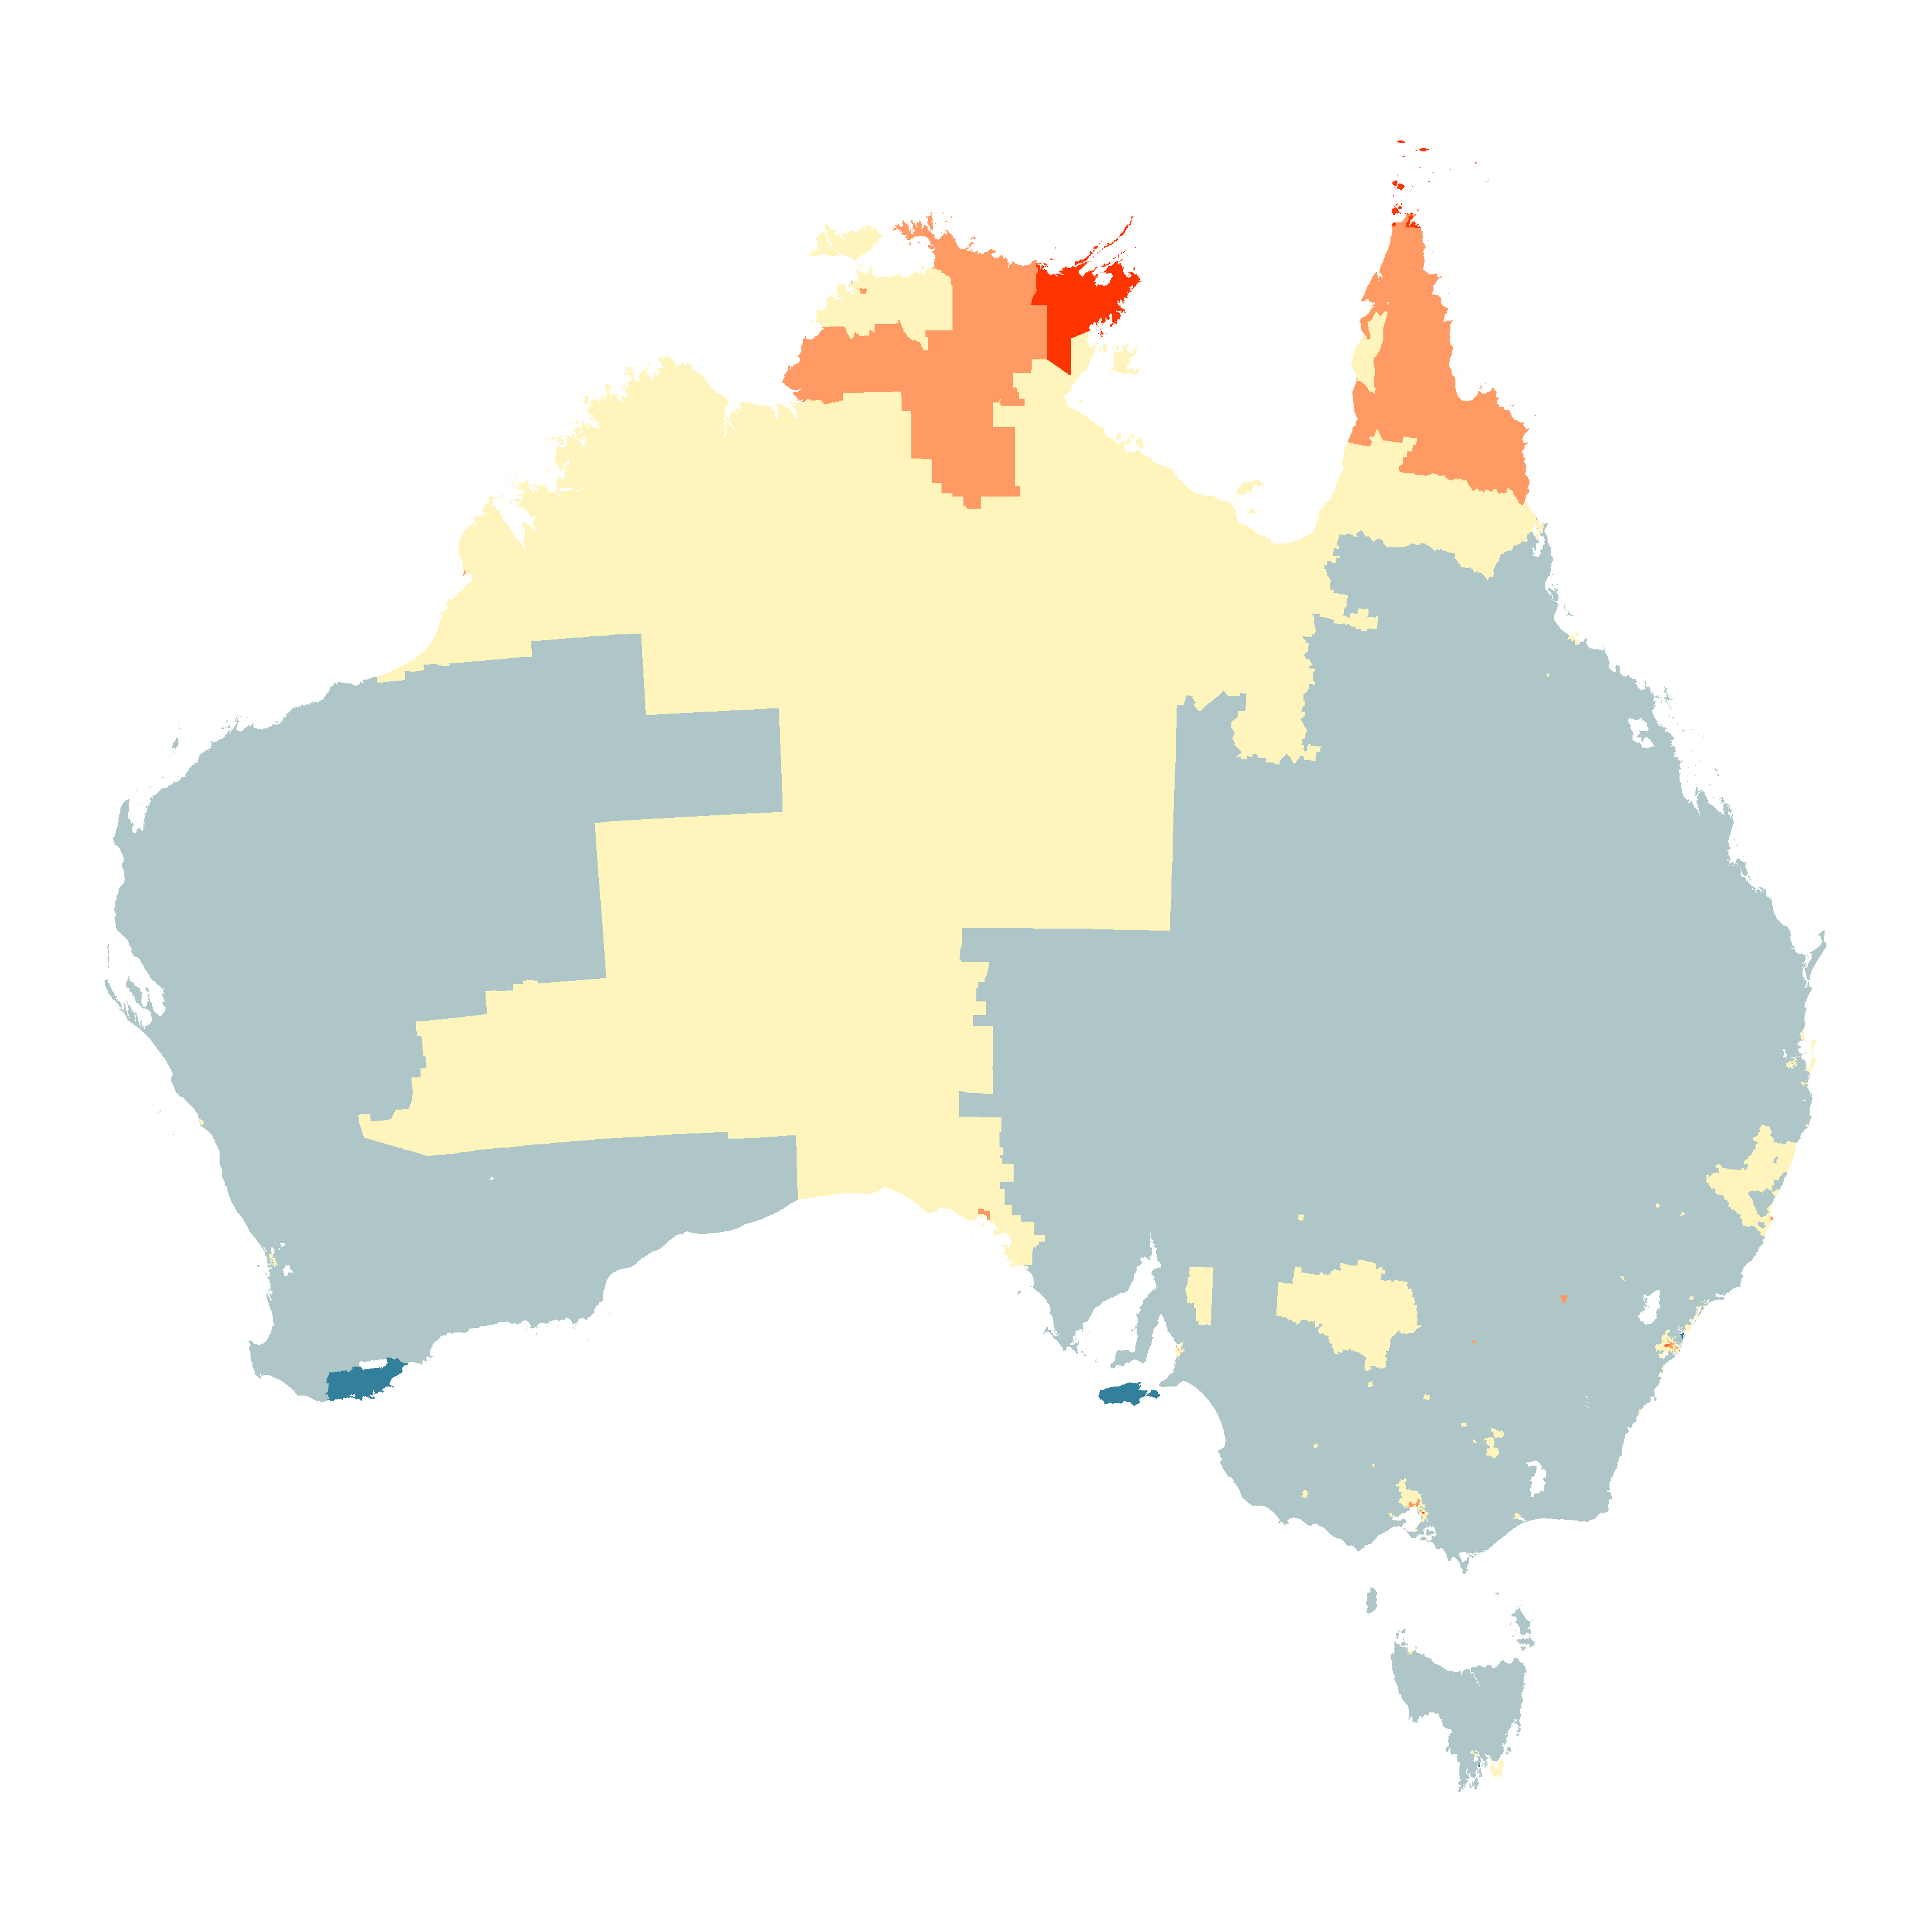
\includegraphics[width=16cm]{figures/04-experiment/aus_liver_m.png}
\caption{\label{fig:liver-geo}A choropleth map of the smoothed average of liver cancer diagnoses for Australian males. The diverging colour scheme uses dark blue areas for much lower than average diagnoses, yellow areas with diagnoses around the Australian average, red shows diagnoses much higher than average. The hexagon tile map shows concentrations of higher than expected liver cancer rates in the cities of Melbourne and Sydney, which is not visible from the choropleth.}
\end{figure}

\begin{figure}[H]
\centering
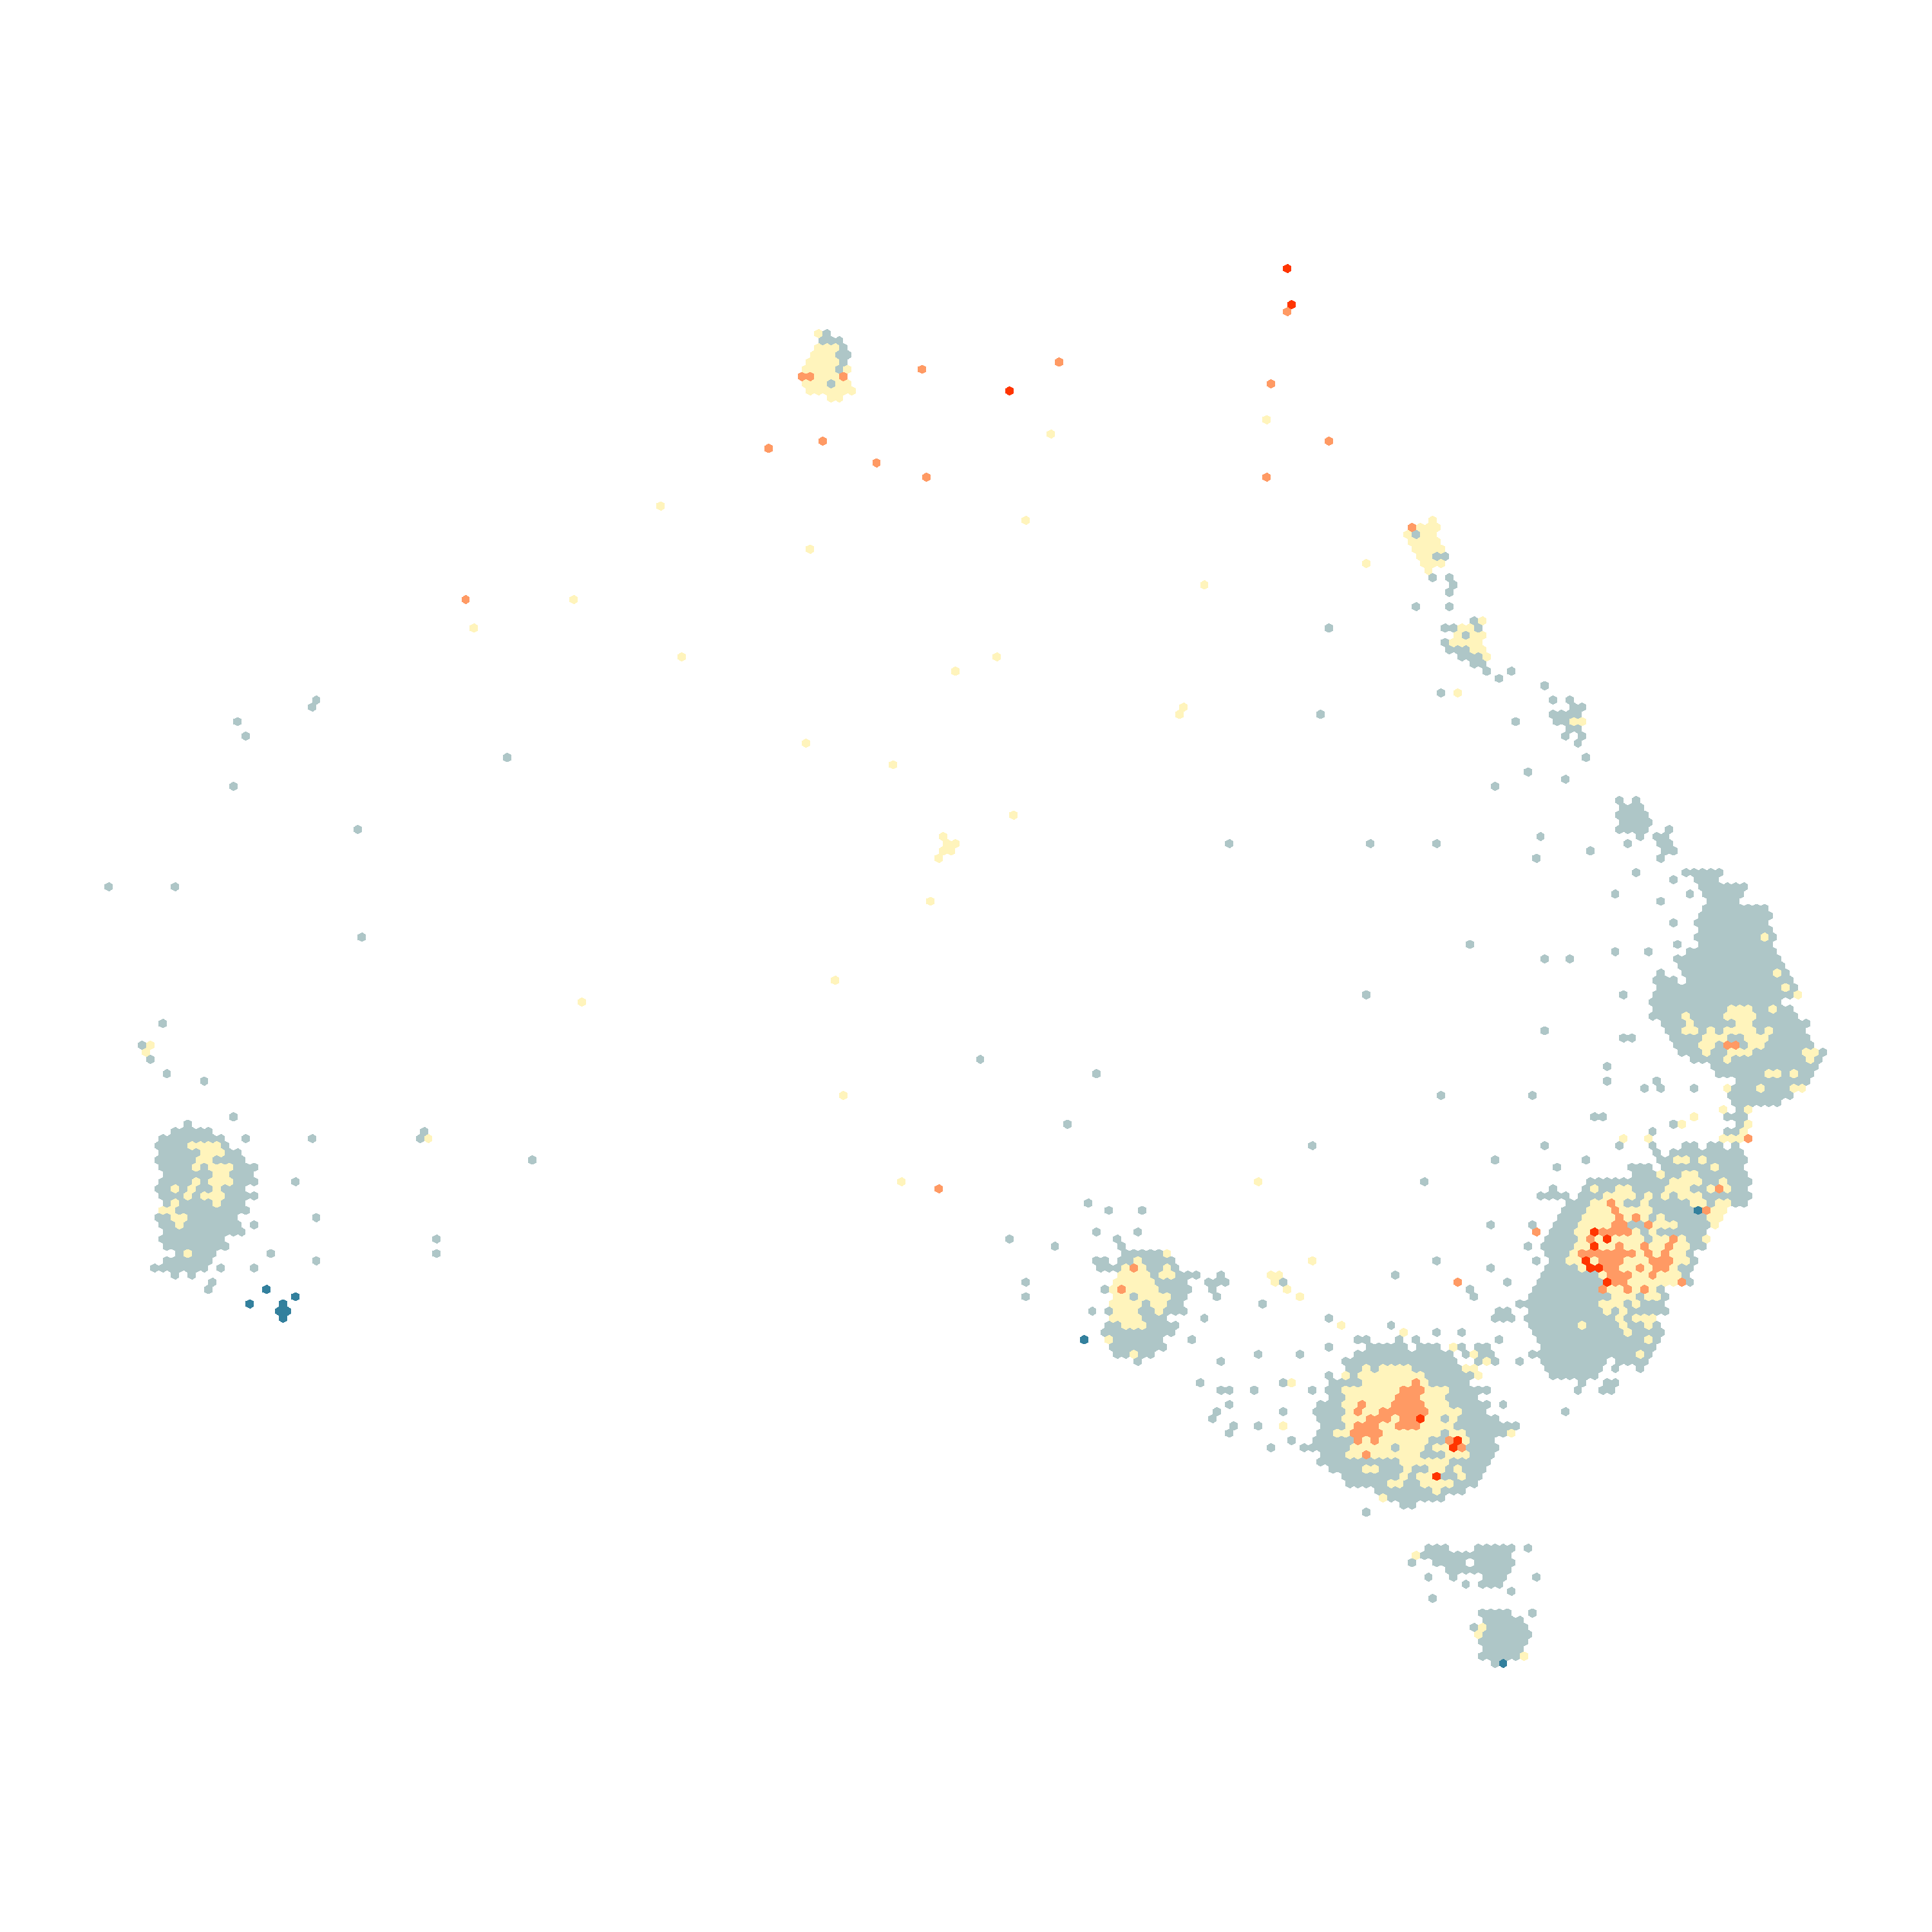
\includegraphics[width=16cm]{figures/04-experiment/aus_liver_m_hex.png}
\caption{\label{fig:liver-hex}A hexagon tile map of the smoothed average of liver cancer diagnoses for Australian males. The diverging colour scheme uses dark blue areas for much lower than average diagnoses, yellow areas with diagnoses around the Australian average, red shows diagnoses much higher than average. The hexagon tile map shows concentrations of higher than expected liver cancer rates in the cities of Melbourne and Sydney, which is not visible from the choropleth.}
\end{figure}

The choropleth map is an effective spatial display if the size of the geographic units is relatively uniform. This is not the case for most countries. Size heterogeneity in administrative units is particularly extreme in Australia: most of the landscape of Australia is sparsely settled, with the population densely clustered into the narrow coastal strips. A choropleth map focuses attention on the geography, and for heterogeneously sized areas it presents a biased view of the population related distribution of the statistic \autocite{CBATCC}. \emph{Land doesn't get cancer, people do} -- a more effective way to communicate the spatial distributions of cancer statistics is needed.

A cartogram is a general solution for better displaying a population-based statistic. It transforms the geographic map base to reflect the population in the geographic region, while preserving some aspects of the geographic location. There are several cartogram algorithms \autocite{ACTUC}, \autocite{CBATCC}; each involves shifting the boundaries of geographic units, using the value of the statistic to increase or decrease the area taken by the geographic unit on the map. The changes to the boundaries result in cartograms that accurately communicate population by map area for each of the geographic units but can result in losing the familiar geographic information. For Australia, the transformations warp the country so that it is no longer recognizable.

Alternative algorithms make various trade offs between familiar shapes and representation of geographic units. The non-contiguous cartogram method \autocite{NAC} keeps the shapes of geographic units intact, and changes the size of the shape. This method disconnects areas creating empty space on the display losing the continuity of the spatial display of the statistic. The Dorling cartogram \autocite{ACTUC} represents each unit as a circle, sized according to the value of the statistic. The neighbour relationships are mostly maintained by how the circles touch. A similar approach was pioneered by Raisz \autocite*{RSCW}, using rectangles that tile to align borders of neighbours \autocite{CDWCS}. There have been thorough reviews of the array of methods, as suitable for cancer atlas displays \autocite{review}, \autocite{BCM}.

The hexagon tile map algorithm, automatically matches spatial regions to their nearest hexagon tile, from a grid of tiles. It has the effect of spreading out the inner city areas while maintaining the spatial locations or regions in remote areas. The algorithm is available in the R package, sugarbag \autocite{sugarbag}. Fig. \ref{fig:liver-geo} shows the hexagon tile map, along with the choropleth map of liver cancer rates in Australia. Colour maps from substantially below average (blue) to substantially above average (red) rates. The inner city areas have expanded, making it possible to see the cancer incidence in the small, densely populated areas. Remote regions are represented by isolated hexagons, which is not ideal, but maintains the spatial location of these data values. It is of interest to know how well the spatial distribution is perceived for this display, in comparison to the choropleth.

\hypertarget{visual-inference}{%
\subsection{Visual Inference}\label{visual-inference}}

In order to assess the effectiveness of the hexagon tile map, the lineup protocol \autocite{GIIV},\autocite{BCHLLSW09} from visual inference procedures is employed. The approach mirrors classical statistical inference. The procedures for doing a power comparison of competing plot designed, outlined in \textcite{GTPCCD}, are followed.

In classical statistical inference hypothesis testing is conducted by comparing the value of a test statistic on a standard reference distribution, computed assuming the null hypothesis is true. If the value is extreme, the null hypothesis is rejected, because the test statistic value is unlikely to have been so extreme if it was true. In the lineup protocol, the plot plays the role of the test statistic, and the data plot is embedded in a field of null plots. Defining the plot using a grammar of graphics \autocite{ggplot2} makes it a functional mapping of the variables and thus, it can be considered to be a statistic. With the same data, two different plots can be considered to be competing statistics, one possibly a more powerful statistic than the other.

To do hypothesis testing with the lineup protocol requires human evaluation. The human judge is required to identify the most different plot among the field of plots. If this corresponds to the data plot -- the test statistic -- the null hypothesis is rejected. It means that the data plot is extreme relative to the reference distribution of null plots.

The null hypothesis is explicitly provided by the grammatical plot description. For example, if a histogram is the plot type being used, the null might be that the underlying distribution of the data is a Gaussian. Null data would be generated by simulating from a normal model, with the same mean and standard deviation as the data. In practice, the null hypothesis used is generic, such as \emph{there is NO structure or a pattern in the plot}, and contrasted to an alternative that there is structure.

The chance that an observer picks the data plot out of a lineup of size \(m\) plots accidentally, if the null hypothesis is true is \(1/m\). With \(K\) observers, the probability of \(k\) randomly choosing the data plot, roughly follows a binomial distribution with \(p=1/m\). Fig. \ref{fig:lineup} shows a lineup of the hexagon tile map, of size \(m=12\). Plot 3 is the data plot, and the remaining 11 are plots of null data.

\begin{figure}[H]
\centering
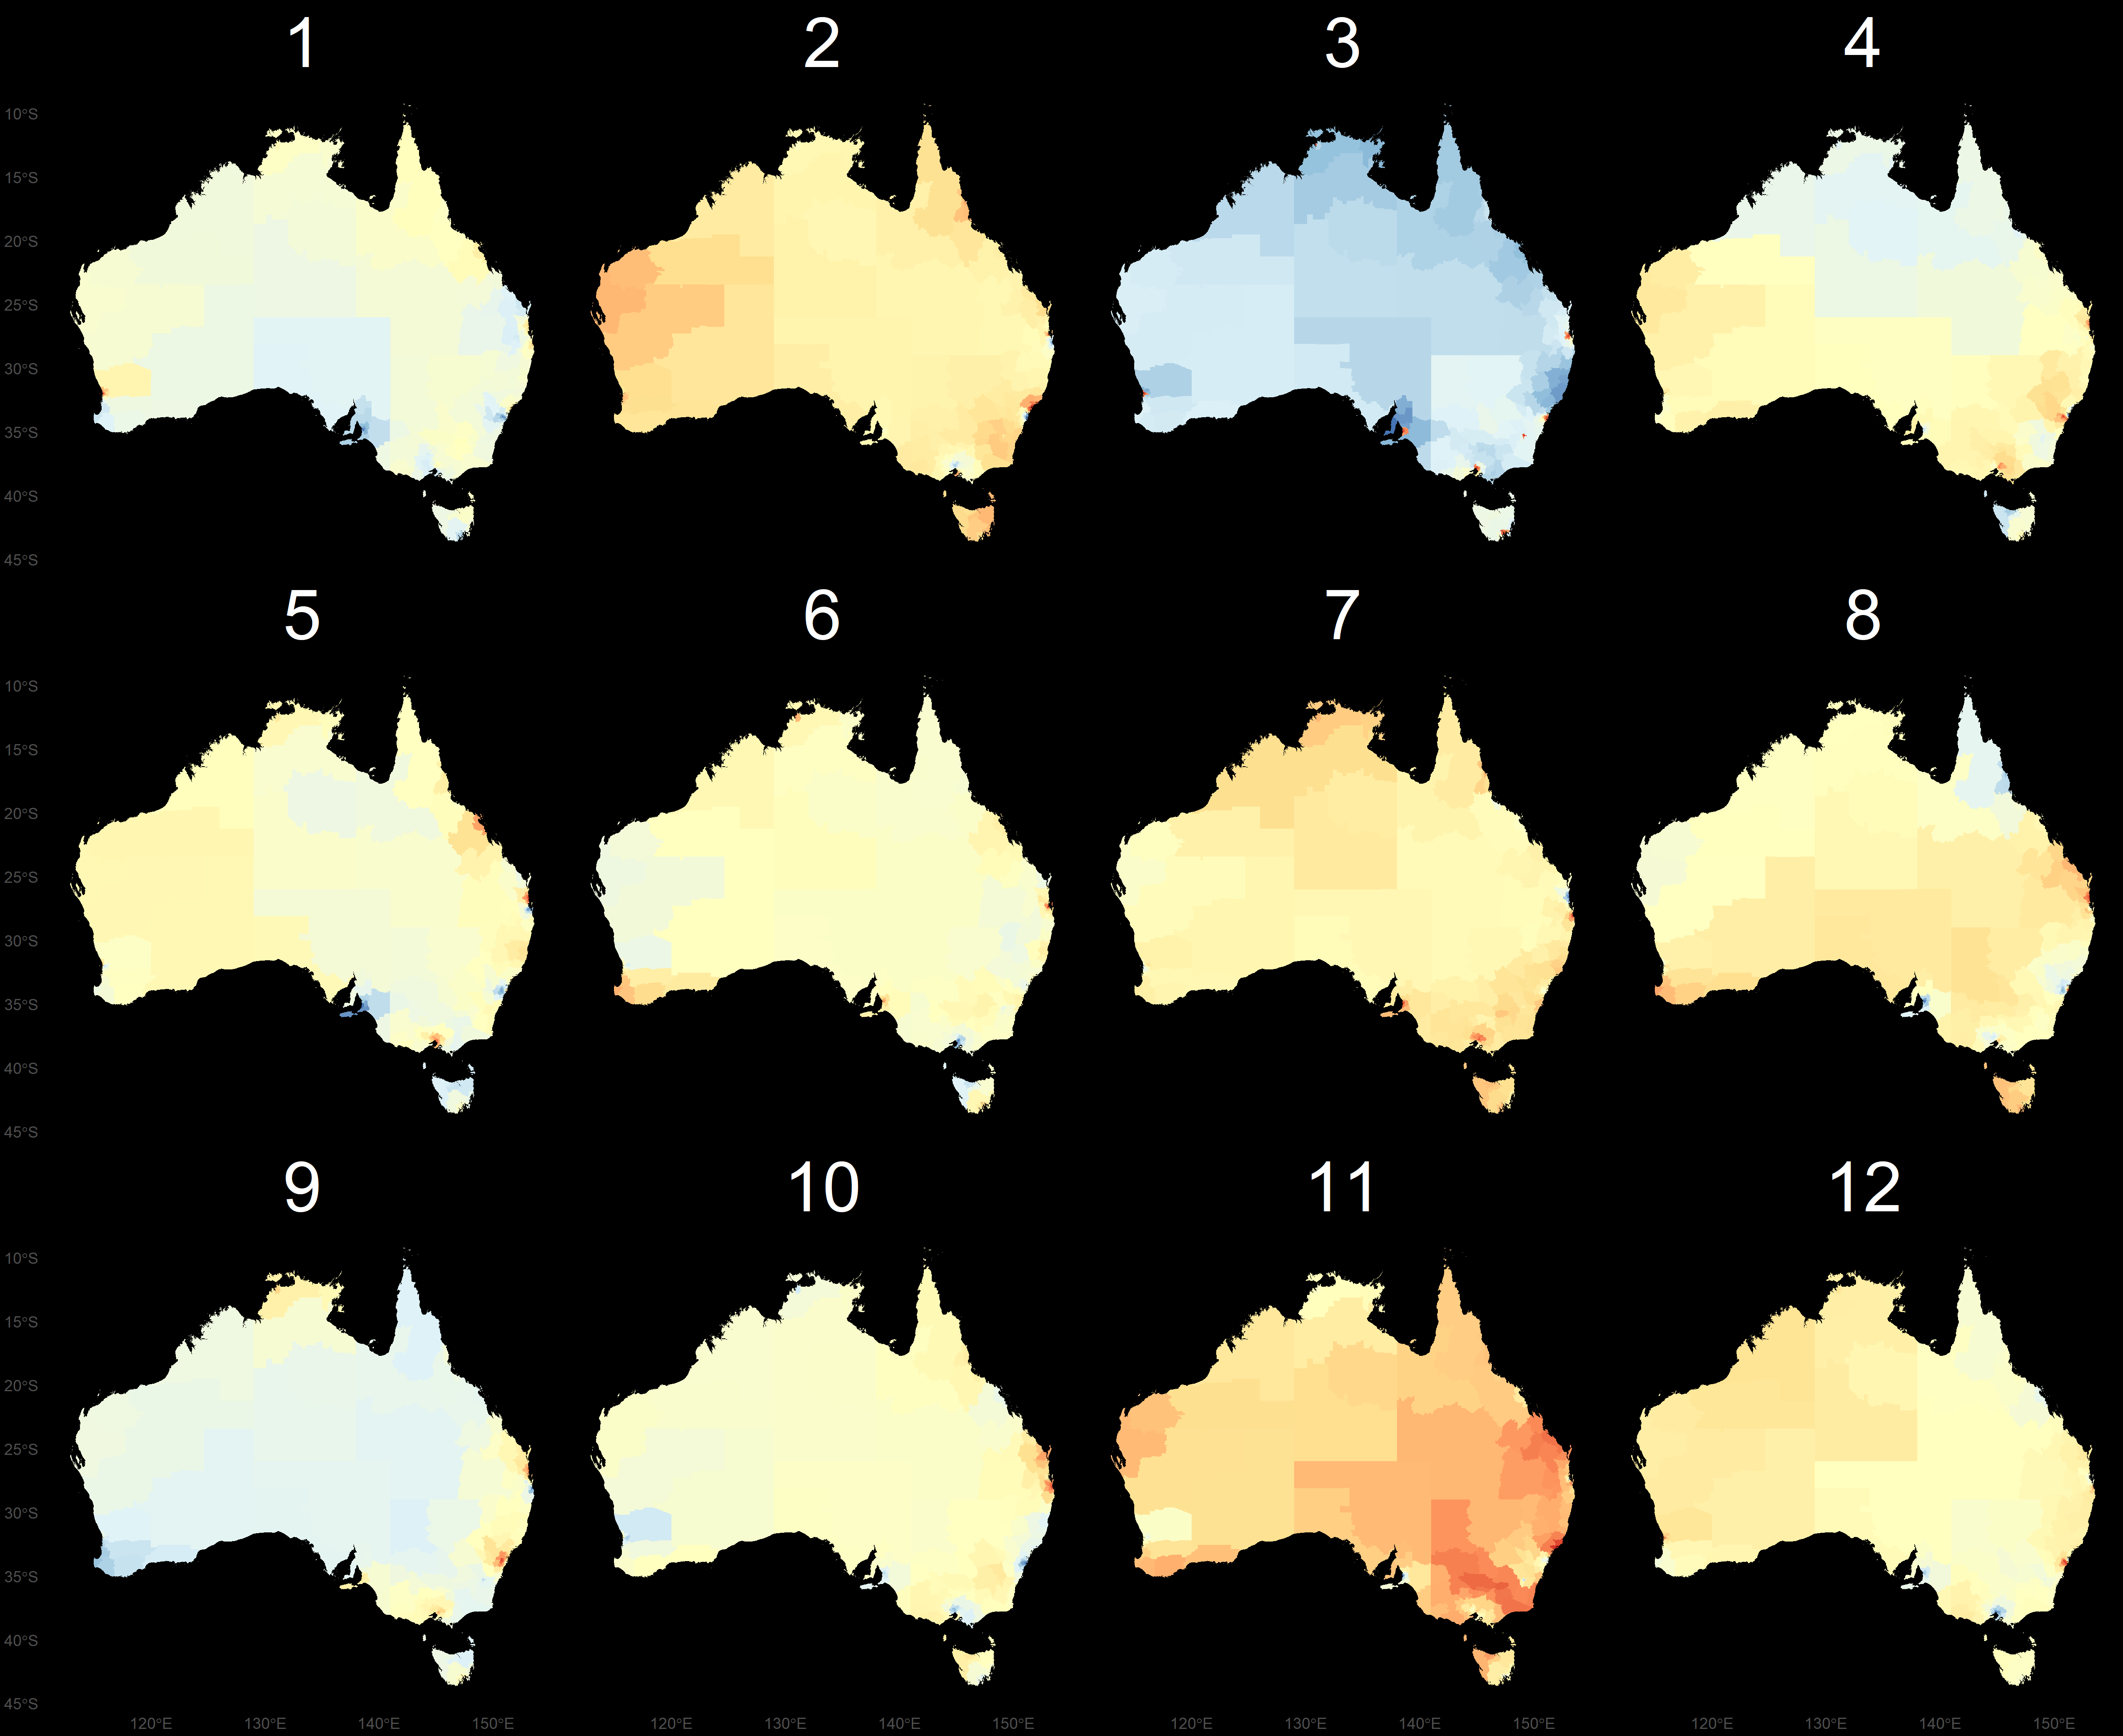
\includegraphics[width=16cm]{figures/04-experiment/aus_cities_3_geo.png}
\caption{\label{fig:lineup}This lineup of twelve hexagon tile map displays contains one map with a real population related structure. The rest are null plots that contain spatial correlation between neighbours.}
\end{figure}

In order to determine the effectiveness of a type of display, this probability is less relevant than the overall proportion of observers who pick the data plot, \(k/K\). The power of the test statistic (data plot) is provided by this proportion. Power in a statistical sense is the ability of the statistic to \emph{produce a rejection} of the null hypothesis, if it is indeed \emph{not true}. With the same data plotted using two different displays, the display with the highest proportion of people who choose the data plot would be considered to be the most powerful statistic.

\hypertarget{methodology}{%
\subsection{Methodology}\label{methodology}}

This study aims to answer two key questions around the presentation of spatial distributions:

\begin{enumerate}
\def\labelenumi{\arabic{enumi}.}
\tightlist
\item
  Are spatial disease trends that impact highly populated small areas detected with higher accuracy, when viewed in a hexagon tile map?
\item
  Are people faster in detecting spatial disease trends that impact highly populated small areas when using a hexagon tile map?
\end{enumerate}

Additional considerations when completing this experimental task included the difficulty experienced by participants and the certainty they had in their decision.

Australia is used for the study, with Statistical Area 3 (SA3) \autocite{abs2016} as the geographic units. The results should apply broadly to any other geographic area of interest.

\hypertarget{experimental-factors}{%
\subsection{Experimental factors}\label{experimental-factors}}

The primary factor in the experiment is the plot type. The secondary factor is a trend model. Three trend models were developed, one mirroring a large spatial trend for which the choropleth would be expected to do well, and two with differing level of inner city hot spots. These latter two reflect the structure seen in the liver cancer data (Fig. \ref{fig:liver-geo}). This produces six treatment levels:

\begin{itemize}
\tightlist
\item
  Map type: \emph{Choropleth, Hexagon tile}
\item
  Trend: \emph{South-East to North-West; Locations in three population centres; Locations in multiple population centres, }
\end{itemize}

Data is generated for each of the trend models, with four replicates, and each displayed both as a choropleth and as a hexagon tile map, which yields 12 data sets, and 24 data plots. This set of displays is divided in half, providing two sets of 12 displays, Group A and Group B. Participants were randomly allocated to Group A or B. Participants saw a data set only once, either as a choropleth or as a hexagon tile map. Table \ref{fig:exp-design} summarises the design and the allocation of the displays.

\begin{figure}[H]
\centering
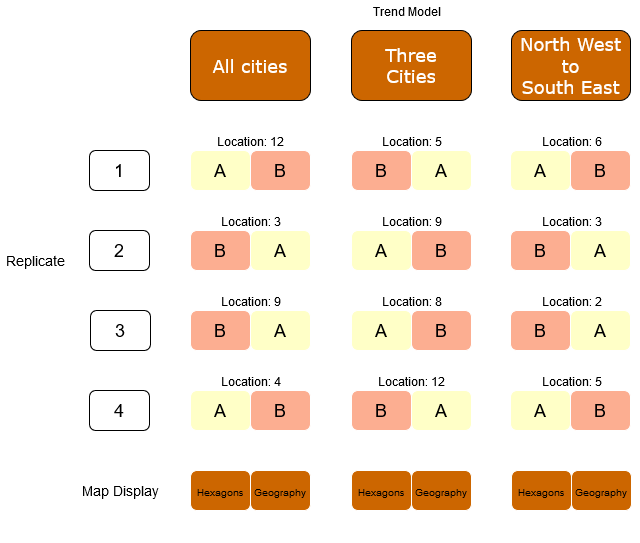
\includegraphics[width=16cm]{figures/04-experiment/experiment_design.png}
\caption{\label{fig:exp-design}The experimental design used in the visual inference study.}
\end{figure}

\hypertarget{generating-null-data}{%
\subsection{Generating null data}\label{generating-null-data}}

Null data needs to be data with no (interesting) structure. In most scenarios, permutation is the main approach for generating null plots. It is used to break association between variables, while maintaining marginal distributions. This is too simple for spatial data. In spatial data, a key feature is the spatial dependence or smoothness over the landscape. To do something simple, like permute the values relative to the geographic location would produce null plots which are too chaotic, and the data plot will be recognisable for its smoothness rather than any structure of interest.

For spatial data, null data is stationary data, where the mean, variance and spatial dependence are constant over the geographic units. Stationary data is specified by a variogram model \autocite{POG}. Simulating from a variogram model, where the spatial dependence is specified, generates the stationary spatial data used for the null plots. The parameters for the Gaussian model were sill=1, range=0.3 with the variance generated by a standard normal distribution.

The R package \texttt{gstat} \autocite{gstat} was used to simulate 144 null sets, 12 data sets for each plot in a lineup, and 12 sets for 12 lineups.

The null model imposed by our hypothesis suggests that neighbors are related. The randomness induced when generating the null data was smoothed to mirror the practices employed by the Australian Cancer Atlas statisticians.
In these 12 sets of data, each of the 12 maps were smoothed several times to replicate the spatial autocorrelation seen in cancer data sets presented in the Australian Cancer Atlas, without implementing uncertainty via transparency.

A list of neighbors for each geographic unit was generated to use when smoothing the distributions. For each geographic unit the same spatial smoother was applied in each layer of smoothing. It kept half of the units' previous value, and derived the new half as the mean of the values of its neighbors at the previous layer of smoothing.

This smoothing allowed neighbors to be related to each other, but also allowed outliers, and showed distributions similar to the Liver cancer distribution (Fig. \ref{fig:liver-geo}).

\hypertarget{generating-lineups}{%
\subsection{Generating lineups}\label{generating-lineups}}

For each trend model, four real data displays were created by manipulating the centroid values of each of the SA3 geographic units.

The North West to South East (NW-SE) distribution was created using a linear equation of the centroid longitude and latitude values.

The All Cities trend model was created using the distance from the centroid of each geographic unit to the closest capital city in Australia, calculated when creating the hexagon tile map using the sugarbag \autocite{sugarbag} package.
201 of the 336 SA3s were considered greater capital city areas, the values of these areas were increased to create red clusters. The amount was chosen to make clusters around the cities visible in the choropleth display even if they were not overtly noticeable.

A similar selection process was applied to the Three Cities' trend model. However, for each of the four replicates for the Three Cities trend, a random sample of capital cities was taken from Sydney, Brisbane, Melbourne, Adelaide, Perth, and Hobart. Only values of the areas nearest to the three cities were increased to create clusters.

One of the lineup locations was chosen to embed the real trend model map, in each of the four replicates, for the three trend models.
The location was chosen from a sub sample of the 12 possible locations. The chance of reptition using resampling was introduced to prevent participants from inducing the location by elimination, the locations 1, 7, 10 and 11 were not used.

As seen in Fig \ref{fig:exp-design}, the choropleth and hexagon display used the same location for the real data display of the trend model was added to the spatially correlated null values for each lineup.
Each set of lineup data was used to produce a choropleth map lineup and hexagon tile map lineup. These matched pairs were split between Group A and Group B according to the 2 x 3 factor experimental design depicted in \ref{fig:exp-design}.

For each of the 144 individual maps, the values for each geographic area were rescaled to create a similar color scale from deep blue to dark red within each map.
This meant at least one geographic unit was coloured dark blue, and at least one was red, in every map display of every lineup.

For the geographic NW-SE distribution, this resulted in the smallest values of the trend model (blue) occurring in Western Australia, the North West of Australia, and the largest values of the trend model (red) occurring in the South East. This resulted in Tasmania being colored completely red.

For the population related displays, the clusters in the cities appeared more red than the rest of Australia.

\hypertarget{analysis}{%
\subsection{Analysis}\label{analysis}}

\hypertarget{data-cleaning}{%
\subsubsection{Data Cleaning}\label{data-cleaning}}

The first step in the data cleaning process involved checking that survey responses collected for each participants were only included once in the data set.
The data cleaning process also involved filtering out participants' who did not provide at least three unique choices when considering each of the twelve lineups. These participants achieved a detection rate of 0. If participants had made various plot choices for the 12 displays they saw they were still included in the dataset.

\hypertarget{descriptive-statistics}{%
\subsubsection{Descriptive statistics}\label{descriptive-statistics}}

Basic descriptive statistics were used to contrast the detection rate for the two types of displays. Comparison was also made across the trend models, contrasting the mean and standard detection rate for each group, who had seen the different map display type for each replicate.

Side-by-side dot plots were made of accuracy (efficiency) against map type, faceted by trend model type.

Similar plots were made of the feedback and demographic variables - reason for choice, reported difficulty, gender, age, education, having lived in Australia - against the design variables.

Plots will be made in R \autocite{R}, with the \texttt{ggplot2} package \autocite{ggplot2}.

\hypertarget{modelling}{%
\subsubsection{Modelling}\label{modelling}}

The likelihood of detecting the data plot in the lineup can be modelled using a linear mixed effects model.
The R \autocite{R} \texttt{glmer()} function in the \texttt{lme4} \autocite{lme4} package implements generalised linear mixed effect models. The model used includes the two main effects map type and trend model, which gives the fixed effects model to be:

\[\widehat{y_{ij}} = \mu + \tau_i + \delta_j + (\tau\delta)_{ij} + \epsilon_{i,j}, ~~~ i=1,2; ~j=1,2,3\]

where \(y_{ij} = 0, 1\) is the logg odds for whether the subject detected the data plot, \(\mu\) is the overall mean, \(\tau_i, i=1,2\) is the map type effect, \(\delta_j\) is the trend model effect. We are allowing for an interaction between map type and trend model as the response is binary, so a logistic model was used. As each participant provides results from 12 lineups, this model can account for each individual participants' abilities as it includes a subject-specific random intercept.

The model specifies a logistic link, this means the predicted values from the \texttt{glmer} model should be back-transformed to fit between 0 and 1. The predictions \(\widehat{p}(\eta)\) are transformed to be probabilities between 0 and 1 with the link specified below:

\[\widehat{p}(\eta) = \frac{e^{\eta}}{1 + e^{\eta}}\] \label{eq:transform}
\[\eta = f(\tau_i,\delta_j)\]

\hypertarget{web-application-to-collect-responses}{%
\subsection{Web application to collect responses}\label{web-application-to-collect-responses}}

The taipan \autocite{taipan} package for R was used to create the survey web application.
This structure was altered to collect responses regarding participants demographics and their survey responses.
The survey app contained three tabs. Participants were first asked for their demographics their Figure Eight contributor ID, and their consent to the responses being used for analysis. The demographics collected included participants' preferred pronoun, the highest level of education achieved, their age range and whether they had lived in Australia.

After submitting these responses, the survey application switched to the tab of lineups and associated questions. This allowed participants to easily move through the twelve displays and provide their choice, reason for their choice, and level of certainty.

When participants completed the twelve evaluations the survey application triggered a data analysis script. This created a data set with one row per evaluation. Containing the responses to the three questions. The script also added the title of the image, which indicated the type of map display, the type of distribution hidden in the lineup, and the location of the data plot. It also calculated the time taken by participant to view each lineup.

Each participant used the internet to access the survey.
The data transfer from the web application to the data set took place using a secure link to the googlesheet used to store results. The application connected to the googlesheet using the googlesheets \autocite{sheets} R package when participants opened the application, and interacted again when participants chose to submit the survey. At this time it added the participant's responses to the twelve lineup displays as twelve rows of data in the googlesheet.

\hypertarget{participants}{%
\subsection{Participants}\label{participants}}

Participants were recruited from the Figure Eight crowdsourcing platform \autocite{figeight} to evaluate lineups.
The lineup protocol expects that the participants are uninvolved judges with no prior knowledge of the data, to avoid inadvertently affecting results. Potential participants needed to have achieved level 2 or level 3 from prior work on the platform. All participants were at least 18 years old.

Participants were allocated to either group A or group B when they proceeded to the survey web application. There were 92 participants involved in the study. All participants read introductory materials, and were trained using three test displays, to orient them to the evaluation task. All participants who completed the task were compensated \$AUD5 for their time, via the Figure Eight payment system.

A pilot study was conducted in the working group of the Econometrics and Business Statistics Department of Monash University. This allowed us to estimate the effect size, and thus decide on number of participants to collect responses from.

\hypertarget{demographic-data-collection}{%
\subsection{Demographic data collection}\label{demographic-data-collection}}

Each participant answered demographic questions and provided consent before evaluating the lineups.

Demographics were collected regarding the study participants:

\begin{itemize}
\tightlist
\item
  Gender (female / male / other),
\item
  Education level achieved (high school / bachelors / masters / doctorate / other),
\item
  Age range (18-24 / 25-34 / 35-44 / 45-54 / 55+ / other)
\item
  Lived at least for one year in Australia (Yes / No )
\end{itemize}

Participants then moved to the evaluation phase.
The set of images differed for Group A and Group B.
After being allocated to a group, each individual was shown the 12 displays in randomised order.

Three questions were asked regarding each display:

\begin{itemize}
\tightlist
\item
  Plot choice
\item
  Reason
\item
  Difficulty
\end{itemize}

After completing the 12 evaluations, the participants were asked to submit their responses.

\hypertarget{results}{%
\section{Results}\label{results}}

Responses from 92 participants were collected. Five participants did not provide more than three unique choices for the twelve lineups, and their data was removed. Set A was evaluated by 42 participants, and 53 evaluated set B. This resulted in 1104 evaluations, corresponding to 92 subjects, each evaluating 12 lineups, that were analysed on accuracy and speed. The certainty and reasons of subjects in their answers is also examined.

\hypertarget{participant-demographics}{%
\subsection{Participant demographics}\label{participant-demographics}}

Of the 92 participants, 67 were male, and 25 female. Most participants (56) had a Bachelors degree, 13 had a Masters degree, and the remaining 23 had high school diplomas.

\hypertarget{accuracy}{%
\subsection{Accuracy}\label{accuracy}}

Fig. \ref{fig:detect-compare} displays the average detection rates for the two types of plot separately for each trend model. Each trend model was tested using four repetitions, evaluations on the same data set were seen as either choropleths or hexagon tile maps by each group as specified in Table. \ref{fig:exp-design}; the detection rates for each display are connected by a line segment. The Three Cities and All Cities trend models shown in the hexagon tile map allowed viewers to detect the data plot substantially more often than the choropleth counterparts. One replicate for the All Cities group had similar detection rates for both plot types, the rate of detection using the choropleth map was much higher than other replicates. Surprisingly, participants could also detect the gradual spatial trend in the NW-SE group from the hexagon tile map. We expected that the choropleth map would be superior for the type of spatial pattern, but the data suggests the hexagon tile map performs slightly better, or equally as well.

\begin{Shaded}
\begin{Highlighting}[]
\CommentTok{## Detectability rate for each lineup (image)}
\NormalTok{d_smry <-}\StringTok{ }\NormalTok{d }\OperatorTok\StringTok{ }\KeywordTok{group_by}\NormalTok{(trend, type, replicate) }\OperatorTok
\StringTok{  }\CommentTok{## pdetect measures the aggregated accuracy of the choices}
\StringTok{  }\KeywordTok{summarise}\NormalTok{(}\DataTypeTok{pdetect =} \KeywordTok{length}\NormalTok{(detect[detect }\OperatorTok{==}\StringTok{ }\DecValTok{1}\NormalTok{])}\OperatorTok{/}\KeywordTok{length}\NormalTok{(detect)) }\OperatorTok
\StringTok{  }\KeywordTok{ungroup}\NormalTok{()}

\CommentTok{## Numerical summary}
\NormalTok{diffs <-}\StringTok{ }\NormalTok{d_smry }\OperatorTok\StringTok{ }\KeywordTok{spread}\NormalTok{(type, pdetect) }\OperatorTok
\StringTok{  }\KeywordTok{mutate}\NormalTok{(}\DataTypeTok{dif =} \StringTok{`}\DataTypeTok{Hex.}\StringTok{`} \OperatorTok{-}\StringTok{ `}\DataTypeTok{Choro.}\StringTok{`}\NormalTok{)}

\CommentTok{## Plot summary}
\KeywordTok{ggplot}\NormalTok{(d_smry, }\KeywordTok{aes}\NormalTok{(}\DataTypeTok{x =}\NormalTok{ type, }\DataTypeTok{y =}\NormalTok{ pdetect, }\DataTypeTok{color =}\NormalTok{ trend)) }\OperatorTok{+}
\StringTok{  }\KeywordTok{geom_point}\NormalTok{(}\DataTypeTok{size =} \DecValTok{2}\NormalTok{) }\OperatorTok{+}\StringTok{  }
\StringTok{  }\KeywordTok{geom_line}\NormalTok{(}\DataTypeTok{size =} \DecValTok{1}\NormalTok{, }\KeywordTok{aes}\NormalTok{(}\DataTypeTok{group =}\NormalTok{ replicate)) }\OperatorTok{+}\StringTok{  }
\StringTok{  }\KeywordTok{facet_wrap}\NormalTok{(}\OperatorTok{~}\NormalTok{trend) }\OperatorTok{+}
\StringTok{  }\KeywordTok{scale_color_manual}\NormalTok{(}\DataTypeTok{values =}\NormalTok{ trend_colors) }\OperatorTok{+}
\StringTok{  }\KeywordTok{xlab}\NormalTok{(}\StringTok{"Type of areas visualized"}\NormalTok{) }\OperatorTok{+}
\StringTok{  }\KeywordTok{ylab}\NormalTok{(}\StringTok{"Detection rate"}\NormalTok{) }\OperatorTok{+}\StringTok{ }
\StringTok{  }\KeywordTok{ylim}\NormalTok{(}\DecValTok{0}\NormalTok{,}\DecValTok{1}\NormalTok{) }\OperatorTok{+}
\StringTok{  }\KeywordTok{guides}\NormalTok{(}\DataTypeTok{color =} \OtherTok{FALSE}\NormalTok{)}
\end{Highlighting}
\end{Shaded}

\begin{figure}
\centering
\includegraphics{thesis_files/figure-latex/detect-compare-1.pdf}
\caption{\label{fig:detect-compare}The detection rates achieved by participants are contrasted when viewing the four replicates of the three trend models. Each point shows the probability of detection for the lineup display, the facets separate the trend models hidden in the lineup. The points for the same data set shown in a choroleth or hexagon tile map display are linked to show the difference in the detection rate.}
\end{figure}

Table. \ref{tab:desc-stats} shows the means and standard deviations of the detection rate for each type of plot and each trend model. This also gives the standard deviations, the smallest standard deviation for all sets of replicates was the Three Cities trend model shown in a Choropleth display. This group of displays had a very small detection rate of 0.04. The mean detection rate for the Three Cities trend model shown as choropleth map lineups was also the smallest at 0.40.
The North-West to South-East (NW-SE) trend model unexpectedly had a higher mean detection rate for the hexagon tile map displays, but the difference in the means of detection rate was only 0.10.

\begin{Shaded}
\begin{Highlighting}[]
\NormalTok{types <-}\StringTok{ }\KeywordTok{c}\NormalTok{(}\StringTok{"Choro."}\NormalTok{, }\StringTok{""}\NormalTok{, }\StringTok{"Hex."}\NormalTok{, }\StringTok{""}\NormalTok{)}

\NormalTok{d }\OperatorTok\StringTok{ }\KeywordTok{group_by}\NormalTok{(type, trend) }\OperatorTok
\StringTok{  }\KeywordTok{summarise}\NormalTok{(}\DataTypeTok{m =} \KeywordTok{as.character}\NormalTok{(}\KeywordTok{round}\NormalTok{(}\KeywordTok{mean}\NormalTok{(detect), }\DecValTok{2}\NormalTok{)),}
      \DataTypeTok{std.dev =} \KeywordTok{as.character}\NormalTok{(}\KeywordTok{round}\NormalTok{(}\KeywordTok{sd}\NormalTok{(detect), }\DecValTok{2}\NormalTok{))) }\OperatorTok\StringTok{ }
\StringTok{  }\KeywordTok{mutate}\NormalTok{(}\DataTypeTok{std.dev =} \KeywordTok{ifelse}\NormalTok{(std.dev }\OperatorTok{==}\StringTok{ }\FloatTok{0.5}\NormalTok{, }\StringTok{"(0.50)"}\NormalTok{, }\KeywordTok{paste0}\NormalTok{(}\StringTok{"("}\NormalTok{, std.dev, }\StringTok{")"}\NormalTok{))) }\OperatorTok\StringTok{   }\KeywordTok{mutate}\NormalTok{(}\DataTypeTok{m =} \KeywordTok{ifelse}\NormalTok{(m }\OperatorTok{==}\StringTok{ }\FloatTok{0.4}\NormalTok{, }\StringTok{"0.40"}\NormalTok{, m)) }\OperatorTok\StringTok{ }
\StringTok{  }\KeywordTok{gather}\NormalTok{(stat, value, m, std.dev) }\OperatorTok\StringTok{ }
\StringTok{  }\KeywordTok{pivot_wider}\NormalTok{(}\DataTypeTok{names_from =} \StringTok{"trend"}\NormalTok{, }\DataTypeTok{values_from =} \StringTok{"value"}\NormalTok{) }\OperatorTok\StringTok{ }
\StringTok{  }\KeywordTok{arrange}\NormalTok{(type) }\OperatorTok\StringTok{ }\KeywordTok{ungroup}\NormalTok{() }\OperatorTok\StringTok{ }
\StringTok{  }\KeywordTok{mutate}\NormalTok{(}\DataTypeTok{Type =}\NormalTok{ types) }\OperatorTok\StringTok{ }\KeywordTok{select}\NormalTok{(Type, }\StringTok{`}\DataTypeTok{NW-SE}\StringTok{`}\NormalTok{, }\StringTok{`}\DataTypeTok{Three Cities}\StringTok{`}\NormalTok{, }\StringTok{`}\DataTypeTok{All Cities}\StringTok{`}\NormalTok{) }\OperatorTok
\StringTok{  }\NormalTok{knitr}\OperatorTok{::}\KeywordTok{kable}\NormalTok{(., }\DataTypeTok{format =} \StringTok{"latex"}\NormalTok{, }\DataTypeTok{align =} \StringTok{"lccc"}\NormalTok{, }\DataTypeTok{booktabs =} \OtherTok{TRUE}\NormalTok{, }
    \DataTypeTok{linesep =} \KeywordTok{c}\NormalTok{(}\StringTok{""}\NormalTok{, }\StringTok{"}\CharTok{\textbackslash{}\textbackslash{}}\StringTok{addlinespace"}\NormalTok{),}
    \DataTypeTok{caption =} \StringTok{"The mean and standard deviation of the rate of detection for each trend model, calculated for the choropleth and hexagon tile map displays."}\NormalTok{)}
\end{Highlighting}
\end{Shaded}

\begin{table}

\caption{\label{tab:desc-stats}The mean and standard deviation of the rate of detection for each trend model, calculated for the choropleth and hexagon tile map displays.}
\centering
\begin{tabular}[t]{lccc}
\toprule
Type & NW-SE & Three Cities & All Cities\\
\midrule
Choro. & 0.52 & 0.04 & 0.23\\
 & (0.50) & (0.19) & (0.42)\\
\addlinespace
Hex. & 0.62 & 0.40 & 0.58\\
 & (0.49) & (0.49) & (0.49)\\
\bottomrule
\end{tabular}
\end{table}

Table. \ref{tab:detect-glmer1} presents a summary of the generalised linear mixed effects model, testing the effect of plot type and trend model on the detection rate. The results support the summary from Fig. \ref{fig:detect-compare} and all parameters are statistically significant despite the large standard deviations observed in Table. \ref{tab:desc-stats}. Overall, the hexagon tile map performs marginally better than the choropleth for all trend models, which is a pleasant surprise. Allowing for the interaction effect, the difference in detection rate decreases for population related displays for a choropleth map lineup, but increases for a hexagon tile map display.
The log odds of detection show in Table. \ref{tab:detect-glmer1} can be back transformed after taking the sum of all terms for the trend and type of display that are of interest.
For the NW-SE distribution, the predicted detection rate for the hexagon tile map display increases the predicted probability of detection to 0.63 from 0.52 for choropleths, this is almost exactly the difference seen in the table of means and is significant only at the 0.05 level.

When a choropleth map display is used, the predicted detection rate for the Three Cities trend, 0.03; this is extremely low, especially compared to the NW-SE trend of 0.52.
When the All Cities trend is presented in a choropleth display the predicted probability of detection is 0.22.
The hexagon tile map has a substantially high detection rate for the display of a Three Cities trend 0.39 and All Cities trend 0.59.

\begin{Shaded}
\begin{Highlighting}[]
\CommentTok{## Mixed effects models}
\NormalTok{glmer1 <-}\StringTok{ }\KeywordTok{glmer}\NormalTok{(detect }\OperatorTok{~}\StringTok{ }\NormalTok{type}\OperatorTok{*}\NormalTok{trend }\OperatorTok{+}\StringTok{ }\NormalTok{(}\DecValTok{1}\OperatorTok{|}\NormalTok{contributor), }
              \DataTypeTok{family =}\NormalTok{ binomial, }\DataTypeTok{data =}\NormalTok{ d)}

\NormalTok{glmer_terms <-}\StringTok{ }\KeywordTok{c}\NormalTok{(}\StringTok{"Intercept"}\NormalTok{, }\StringTok{"Hex."}\NormalTok{, }\StringTok{"Three Cities"}\NormalTok{, }\StringTok{"All Cities"}\NormalTok{,}
  \StringTok{"Hex:Three Cities"}\NormalTok{, }\StringTok{"Hex:All Cities"}\NormalTok{)}

\NormalTok{detection_rates <-}\StringTok{ }\KeywordTok{tidy}\NormalTok{(glmer1) }\OperatorTok
\StringTok{  }\KeywordTok{mutate}\NormalTok{(}\DataTypeTok{detection_rates =} \KeywordTok{round}\NormalTok{(}\KeywordTok{exp}\NormalTok{(estimate)}\OperatorTok{/}\NormalTok{(}\DecValTok{1}\OperatorTok{+}\KeywordTok{exp}\NormalTok{(estimate)),}\DecValTok{2}\NormalTok{)) }\OperatorTok
\StringTok{  }\KeywordTok{select}\NormalTok{(term, estimate, detection_rates) }\OperatorTok\StringTok{ }\KeywordTok{pull}\NormalTok{(detection_rates)}

\KeywordTok{tidy}\NormalTok{(glmer1) }\OperatorTok
\StringTok{  }\KeywordTok{mutate_at}\NormalTok{(}\DataTypeTok{.vars =} \KeywordTok{c}\NormalTok{(}\StringTok{"estimate"}\NormalTok{, }\StringTok{"std.error"}\NormalTok{), round, }\DecValTok{2}\NormalTok{) }\OperatorTok\StringTok{ }
\StringTok{  }\KeywordTok{mutate}\NormalTok{(}\DataTypeTok{p.value =} \KeywordTok{round}\NormalTok{(p.value, }\DataTypeTok{digits=}\DecValTok{2}\NormalTok{)) }\OperatorTok\StringTok{ }
\StringTok{  }\KeywordTok{rowwise}\NormalTok{() }\OperatorTok
\StringTok{  }\KeywordTok{mutate}\NormalTok{(}\DataTypeTok{sig =} \KeywordTok{case_when}\NormalTok{(}
\NormalTok{  p.value }\OperatorTok{<=}\StringTok{ }\FloatTok{0.001} \OperatorTok{~}\StringTok{ "$^\{***\}$"}\NormalTok{,}
\NormalTok{  p.value }\OperatorTok{<=}\StringTok{ }\FloatTok{0.01} \OperatorTok{~}\StringTok{  "$^\{**\}$"}\NormalTok{,}
\NormalTok{  p.value }\OperatorTok{<=}\StringTok{ }\FloatTok{0.05} \OperatorTok{~}\StringTok{  "$^\{*\}$"}\NormalTok{,}
\NormalTok{  p.value }\OperatorTok{<=}\StringTok{ }\FloatTok{0.01} \OperatorTok{~}\StringTok{  "$^\{.\}$"}\NormalTok{,}
  \OtherTok{TRUE} \OperatorTok{~}\StringTok{ "$^\{ \}$"}\NormalTok{)) }\OperatorTok
\StringTok{  }\KeywordTok{ungroup}\NormalTok{() }\OperatorTok\StringTok{ }
\StringTok{  }\KeywordTok{filter}\NormalTok{(}\OperatorTok{!}\KeywordTok{is.na}\NormalTok{(std.error)) }\OperatorTok
\StringTok{  }\KeywordTok{mutate}\NormalTok{(}\DataTypeTok{term =}\NormalTok{ glmer_terms) }\OperatorTok\StringTok{ }
\StringTok{  }\KeywordTok{select}\NormalTok{(}\DataTypeTok{Term =}\NormalTok{ term, }
    \DataTypeTok{Est. =}\NormalTok{ estimate, }
    \DataTypeTok{Sig. =}\NormalTok{ sig,}
    \StringTok{`}\DataTypeTok{Std. Error}\StringTok{`}\NormalTok{ =}\StringTok{ }\NormalTok{std.error, }
    \StringTok{`}\DataTypeTok{P val}\StringTok{`}\NormalTok{ =}\StringTok{ }\NormalTok{p.value) }\OperatorTok\StringTok{ }
\StringTok{  }\NormalTok{knitr}\OperatorTok{::}\KeywordTok{kable}\NormalTok{(}\DataTypeTok{format =} \StringTok{"latex"}\NormalTok{, }\DataTypeTok{escape =} \OtherTok{FALSE}\NormalTok{, }\DataTypeTok{align=} \StringTok{"rrlrr"}\NormalTok{, }
    \DataTypeTok{booktabs =}\NormalTok{ T, }\DataTypeTok{linesep =} \KeywordTok{c}\NormalTok{(}\StringTok{""}\NormalTok{, }\StringTok{"}\CharTok{\textbackslash{}\textbackslash{}}\StringTok{addlinespace"}\NormalTok{, }\StringTok{""}\NormalTok{, }\StringTok{"}\CharTok{\textbackslash{}\textbackslash{}}\StringTok{addlinespace"}\NormalTok{, }\StringTok{""}\NormalTok{), }
    \DataTypeTok{caption =} \StringTok{"The model output for the generalised linear mixed effect model for detection rate. This model considers the type of display, the trend model hidden in the data plot, and accounts for contributor performance."}\NormalTok{)}
\end{Highlighting}
\end{Shaded}

\begin{table}

\caption{\label{tab:detect-glmer1}The model output for the generalised linear mixed effect model for detection rate. This model considers the type of display, the trend model hidden in the data plot, and accounts for contributor performance.}
\centering
\begin{tabular}[t]{rrlrr}
\toprule
Term & Est. & Sig. & Std. Error & P val\\
\midrule
Intercept & 0.07 & $^{ }$ & 0.16 & 0.67\\
Hex. & 0.46 & $^{*}$ & 0.22 & 0.04\\
\addlinespace
Three Cities & -3.41 & $^{***}$ & 0.42 & 0.00\\
All Cities & -1.34 & $^{***}$ & 0.24 & 0.00\\
\addlinespace
Hex:Three Cities & 2.44 & $^{***}$ & 0.47 & 0.00\\
Hex:All Cities & 1.16 & $^{***}$ & 0.33 & 0.00\\
\bottomrule
\end{tabular}
\end{table}

\hypertarget{speed}{%
\subsection{Speed}\label{speed}}

Fig. \ref{fig:beeswarm} shows horizontally jittered dot plots to contrast the time taken by participants to evaluate each lineup when viewing each type of display. The time are also separated by trend model and whether the data plot was detected or not detected. The time taken to complete an evaluation ranged from milliseconds to 60 seconds. The average time taken for type of display is shown as a large colored dot on each plot. when considering the heights of the green and orange dots, there is little difference in the average time taken to read a choropleth or hexagon tile map. Comparing the same colored dot across each trend model row, there is a slight increase in the time taken to correctly detected the data plot in the hexagon tile map lineup, but little difference in evaluation time for the choropleth display. However, there were substantially less correct detections for choropleth lineups for the Three cities and All Cities trends.

\begin{Shaded}
\begin{Highlighting}[]
\CommentTok{## Di playing}
\NormalTok{s <-}\StringTok{ }\NormalTok{d }\OperatorTok\StringTok{ }\KeywordTok{group_by}\NormalTok{(type, trend, detect_f) }\OperatorTok
\StringTok{  }\KeywordTok{summarise}\NormalTok{(}\DataTypeTok{m=}\KeywordTok{median}\NormalTok{(time_taken), }
            \DataTypeTok{q1=}\KeywordTok{quantile}\NormalTok{(time_taken, }\FloatTok{0.25}\NormalTok{), }
            \DataTypeTok{q3=}\KeywordTok{quantile}\NormalTok{(time_taken, }\FloatTok{0.75}\NormalTok{))}
\KeywordTok{library}\NormalTok{(ggbeeswarm)}
\KeywordTok{ggplot}\NormalTok{() }\OperatorTok{+}\StringTok{ }
\StringTok{  }\KeywordTok{geom_quasirandom}\NormalTok{(}\DataTypeTok{data=}\NormalTok{d, }\KeywordTok{aes}\NormalTok{(}\DataTypeTok{x=}\NormalTok{type, }\DataTypeTok{y=}\NormalTok{time_taken), }\DataTypeTok{alpha=}\FloatTok{0.9}\NormalTok{) }\OperatorTok{+}\StringTok{ }
\StringTok{  }\CommentTok{#geom_hline(data=s, aes(yintercept=m, color=type)) +}
\StringTok{  }\KeywordTok{geom_point}\NormalTok{(}\DataTypeTok{data=}\NormalTok{s, }\KeywordTok{aes}\NormalTok{(}\DataTypeTok{x=}\NormalTok{type, }\DataTypeTok{y=}\NormalTok{m, }\DataTypeTok{color=}\NormalTok{type), }\DataTypeTok{size=}\DecValTok{5}\NormalTok{, }\DataTypeTok{alpha=}\FloatTok{0.7}\NormalTok{) }\OperatorTok{+}
\StringTok{  }\CommentTok{#geom_errorbar(data=s, aes(x=type, ymin=q1, ymax=q3, color=type), width=0.3, size=2) +}
\StringTok{  }\KeywordTok{scale_color_brewer}\NormalTok{(}\StringTok{""}\NormalTok{, }\DataTypeTok{palette =} \StringTok{"Dark2"}\NormalTok{) }\OperatorTok{+}
\StringTok{  }\KeywordTok{facet_grid}\NormalTok{(trend}\OperatorTok{~}\NormalTok{detect_f) }\OperatorTok{+}\StringTok{ }
\StringTok{  }\KeywordTok{ylab}\NormalTok{(}\StringTok{"Time taken (seconds)"}\NormalTok{) }\OperatorTok{+}\StringTok{ }\KeywordTok{xlab}\NormalTok{(}\StringTok{""}\NormalTok{) }\OperatorTok{+}
\StringTok{  }\KeywordTok{theme}\NormalTok{(}\DataTypeTok{legend.position=}\StringTok{"bottom"}\NormalTok{)}
\end{Highlighting}
\end{Shaded}

\begin{figure}
\centering
\includegraphics{thesis_files/figure-latex/beeswarm-1.pdf}
\caption{\label{fig:beeswarm}The distribution of the time taken (seconds) to submit a response for each combination of trend, whether the data plot was detected, and type of display, shown using horizontally jittered dotplots. The colored point indicates average time taken for each plot type. Although some participants take just a few seconds per evaluation, and some take as much as mcuh as 60 seconds, but there is very little difference in time taken between plot types.}
\end{figure}

\hypertarget{certainty}{%
\subsection{Certainty}\label{certainty}}

Participants provided their level of certainty regarding their choice using a five point scale.
Unlike the accuracy and speed of responses that were derived during the data processing phase, this was a subjective
assessment by the participant prompted by the question: `How certain are you about your choice?'.
Fig. \ref{fig:certainty} shows the amount of times participants provided each level of certainty. This was separated for each combination of trend models and display type, and colored depending on whether a participant correctly detected the data plot in the lineup.
Participants often chose 4 or 5 when viewing the population related trends in the choropelth display, even though they were often incorrect when viewing an All Cities trend and overwhelmingly incorrect for the Three Cities trend. This shows overconfidence in their detection ability when using a choropleth map display. Participants were less likely to be certain when their choice was incorrect and they were viewing a hexagon tile map.
For each trend model, participants were more likely to doubt their choice and choose 1 or 2 in the hexagon tile map displays, even though many had made the correct choice.

\begin{Shaded}
\begin{Highlighting}[]
\NormalTok{d <-}\StringTok{ }\NormalTok{d }\OperatorTok\StringTok{ }
\StringTok{  }\KeywordTok{mutate}\NormalTok{(}\DataTypeTok{certainty =} \KeywordTok{as_factor}\NormalTok{(certainty)) }\OperatorTok\StringTok{ }
\StringTok{  }\KeywordTok{mutate}\NormalTok{(}\DataTypeTok{replicate_f =} \KeywordTok{as_factor}\NormalTok{(replicate)) }
 
\NormalTok{d }\OperatorTok\StringTok{ }
\StringTok{  }\KeywordTok{mutate}\NormalTok{(}\DataTypeTok{Detected =} \KeywordTok{factor}\NormalTok{(detect_f, }
    \DataTypeTok{levels =} \KeywordTok{c}\NormalTok{(}\StringTok{"Detected? Yes"}\NormalTok{, }\StringTok{"Detected? No"}\NormalTok{), }
    \DataTypeTok{labels =} \KeywordTok{c}\NormalTok{(}\StringTok{"Yes"}\NormalTok{, }\StringTok{"No"}\NormalTok{))) }\OperatorTok\StringTok{ }
\KeywordTok{ggplot}\NormalTok{(}\KeywordTok{aes}\NormalTok{(}\DataTypeTok{x =}\NormalTok{ certainty, }\DataTypeTok{fill =}\NormalTok{ Detected)) }\OperatorTok{+}\StringTok{  }
\StringTok{  }\KeywordTok{scale_fill_manual}\NormalTok{(}\DataTypeTok{values =}\NormalTok{ detect_f_colors) }\OperatorTok{+}
\StringTok{  }\KeywordTok{geom_bar}\NormalTok{() }\OperatorTok{+}\StringTok{ }\KeywordTok{facet_grid}\NormalTok{(type }\OperatorTok{~}\StringTok{ }\NormalTok{trend) }\OperatorTok{+}
\StringTok{  }\KeywordTok{theme}\NormalTok{(}\DataTypeTok{legend.position =} \StringTok{"bottom"}\NormalTok{) }\OperatorTok{+}\StringTok{ }\KeywordTok{xlab}\NormalTok{(}\StringTok{"Level of certainty"}\NormalTok{)}
\end{Highlighting}
\end{Shaded}

\begin{figure}
\centering
\includegraphics{thesis_files/figure-latex/certainty-1.pdf}
\caption{\label{fig:certainty}The amount of times each level of certainty was chosen by participants when viewing hexagon tile map or choropleth displays. Participants were more likely to choose a high certainty when considering a Choropleth map. The mid value of 3 was the default certainty, it was chosen most for the Hexagon tile map displays.}
\end{figure}

\hypertarget{reason}{%
\subsection{Reason}\label{reason}}

Participants were asked why they had made their plot choice and were able to select from a set of suggested reasons.
``Color trend across the areas'' was the most common selection for NW-SE trend displays.

The reasons chosen by participants from the list provided to them varied more when viewing choropleth displays than the hexagon tile map.
The hexagon tile map displays resulted in ``Clusters of color'' as the most common choice made by participants.

The choice ``None of these reasons'' was used as the default value to minimise noise from participants who did not select a response.

\begin{Shaded}
\begin{Highlighting}[]
\CommentTok{## Qualitative analysis of reason}
\NormalTok{d }\OperatorTok\StringTok{ }
\StringTok{  }\KeywordTok{mutate}\NormalTok{(}\DataTypeTok{reason =} \KeywordTok{ifelse}\NormalTok{(reason }\OperatorTok{==}\StringTok{"0.0"}\NormalTok{, }\StringTok{"no reason"}\NormalTok{, reason)) }\OperatorTok\StringTok{ }
\StringTok{  }\KeywordTok{mutate}\NormalTok{(}\DataTypeTok{Detected =} \KeywordTok{ifelse}\NormalTok{(detect_f }\OperatorTok{==}\StringTok{ "Detected? Yes"}\NormalTok{, }\StringTok{"Yes"}\NormalTok{, }\StringTok{"No"}\NormalTok{),}
    \DataTypeTok{Trend =}\NormalTok{ trend) }\OperatorTok\StringTok{ }
\StringTok{  }\KeywordTok{group_by}\NormalTok{(Trend, Detected, type) }\OperatorTok\StringTok{ }
\StringTok{  }\KeywordTok{count}\NormalTok{(reason) }\OperatorTok\StringTok{ }
\StringTok{  }\KeywordTok{mutate}\NormalTok{(}\DataTypeTok{prop =} \KeywordTok{round}\NormalTok{(n}\OperatorTok{/}\KeywordTok{sum}\NormalTok{(n), }\DecValTok{2}\NormalTok{), }\DataTypeTok{r_prop =} \KeywordTok{paste0}\NormalTok{(reason, }\StringTok{":"}\NormalTok{, prop)) }\OperatorTok\StringTok{ }
\StringTok{  }\KeywordTok{top_n}\NormalTok{(}\DecValTok{1}\NormalTok{, n) }\OperatorTok\StringTok{ }\KeywordTok{summarise}\NormalTok{(}\DataTypeTok{reasons =} \KeywordTok{paste}\NormalTok{(reason, }\DataTypeTok{collapse=}\StringTok{", "}\NormalTok{)) }\OperatorTok\StringTok{ }
\StringTok{  }\KeywordTok{pivot_wider}\NormalTok{(}\DataTypeTok{names_from =} \KeywordTok{c}\NormalTok{(}\StringTok{"type"}\NormalTok{), }\DataTypeTok{values_from =} \KeywordTok{c}\NormalTok{(}\StringTok{"reasons"}\NormalTok{)) }\OperatorTok\StringTok{ }
\StringTok{  }\KeywordTok{ungroup}\NormalTok{() }\OperatorTok\StringTok{ }
\StringTok{  }\NormalTok{knitr}\OperatorTok{::}\KeywordTok{kable}\NormalTok{(., }\DataTypeTok{format =} \StringTok{"latex"}\NormalTok{, }\DataTypeTok{booktabs =} \OtherTok{TRUE}\NormalTok{,}
    \DataTypeTok{linesep =} \KeywordTok{c}\NormalTok{(}\StringTok{""}\NormalTok{, }\StringTok{"}\CharTok{\textbackslash{}\textbackslash{}}\StringTok{addlinespace"}\NormalTok{, }\StringTok{""}\NormalTok{, }\StringTok{"}\CharTok{\textbackslash{}\textbackslash{}}\StringTok{addlinespace"}\NormalTok{,}\StringTok{""}\NormalTok{),}
    \DataTypeTok{caption =} \StringTok{"The amount of participants that selected each reason for their choice of plot when looking at each trend model shown in Choropleth and Hexagon Tile maps. The facets show whether or not the choice was correct."}\NormalTok{) }\OperatorTok\StringTok{ }
\StringTok{  }\CommentTok{#kable_styling(bootstrap_options = "hold_position") %>% }
\StringTok{  }\KeywordTok{collapse_rows}\NormalTok{(., }\DataTypeTok{columns =} \DecValTok{1}\NormalTok{)}
\end{Highlighting}
\end{Shaded}

\begin{table}

\caption{\label{tab:reason}The amount of participants that selected each reason for their choice of plot when looking at each trend model shown in Choropleth and Hexagon Tile maps. The facets show whether or not the choice was correct.}
\centering
\begin{tabular}[t]{llll}
\toprule
Trend & Detected & Choro. & Hex.\\
\midrule
 & No & trend & clusters\\
\cmidrule{2-4}
\multirow{-2}{*}{\raggedright\arraybackslash NW-SE} & Yes & trend & clusters\\
\cmidrule{1-4}
 & No & trend & clusters\\
\cmidrule{2-4}
\multirow{-2}{*}{\raggedright\arraybackslash Three Cities} & Yes & consistent & clusters\\
\cmidrule{1-4}
 & No & trend & clusters\\
\cmidrule{2-4}
\multirow{-2}{*}{\raggedright\arraybackslash All Cities} & Yes & clusters, consistent & clusters\\
\bottomrule
\end{tabular}
\end{table}

\hypertarget{discussion}{%
\section{Discussion}\label{discussion}}

The intention of this study was to contrast the use of the choropleth map and the hexagon tile map.
The visual inference lineup protocol was employed to contrast the effectiveness of the displays.
The results have shown that overall the use of the hexagon tile map display allows participants to find the data plot in the lineup more often.
Using the visual inference protocol this result can be extended to show that it is a valid alternative display to communicate spatial distributions of population related data.

We expected that the choropleth map would be superior for communicating the spatial pattern of geographic distributions. The data suggest that the participants perform slightly better or equally as well for each replicate in each trend model across the two displays. Table II shows that the difference in the mean detection rate for the two trend models was 0.10.

The differences seen in the \ref{fig:detect-compare} plot and Table. \ref{tab:desc-stats} are reflected in the model results. Surprisingly the difference for the geographic distribution was significant at the 0.05 level.
It also showed that the hexagon tile map display performs marginally better than the choropleth for all trend models. Unexpectedly the detection rate suffers when using a choropleth map to display population related distributions.

While the significance of the difference in detection was the key focus of this experiment, the secondary focus was the time taken by participants. it was expected that the participants may take longer to consider the hexagon tile map distribution but would be able to detect the data plot in the lineup.
The bimodal distributions seen in Fig. \ref{fig:beeswarm} showed very little difference in the mean evaluation times. As the maximum time of all of the distributions approached 60 seconds it cannot be said that the participants' took longer to evaluate the hexagon tile map displays.

The responses to the questions asked of participants included the reason for their choice and the certainty around their choice.
Fig. \ref{tab:reason} shows high levels of certainty of 4 and 5 were chosen by participants when looking at the population distributions in a choropleth map display show that they were over confident when attempting to find the real data plot in the choropleth map displays. Participants performed better on the NW-SE distribution shown in the choropleth display and were reasonably confident about their decisions.
The high levels of the mid range value of 3 could indicate that the participant did not want to provide a response, as this was the default value. Those who chose level 4 or 5 were equally likely to be correct for the three cities lineups, but more likely to be correct than incorrect for the other two trend models.

The color scaling applied in Three cities and All cities displays resulted in the rural areas of the real data plot appearing more blue or yellow than the other plots in the lineups.
Due to the consistent coloring of rural areas in a choropleth display, the choice ``All areas have similar colors'' was most common reason for a participants choice. The All Cities displays colored the inner-city areas of all capital cities more red, this was observable to participants and explains the equal choice of the city clusters or rural color consistency.
Choosing ``Clusters of colour'' was expected when participants viewed the Hexagon tile map display of the All Cities and Three Cities distributions. It was unexpected that it was also the most common reason for the NW-SE hexagon tile map displays.
Due to the spatial covariance introduced in the smoothing, groups of similarly colored hexagons were present in all of the hexagon tile map displays. All Cities and Three Cities distributions of real data trends had distinctly different patterns or red inner-city areas, while some of the plots in each lineup may have shared similar features.

\hypertarget{conclusion-1}{%
\section{Conclusion}\label{conclusion-1}}

The choropleth map display and the tessellated hexagon tile map have been contrasted using the lineup protocol. The hexagon tile map was significantly more effective for spotting a real population related data trend model hidden in a lineup.

The hexagon tile map display should be considered as an alternative visualization method when communicating distributions that relate to the population across a set of geographic units. As an additional display to the familiar choropleth map, cancer atlas products may benefit from the opportunity to allow exploration via an alternative display. The spatial distributions used to test these displays were inspired by the real spatially smoothed estimates of the cancer burden on Australian communities. However, this technique may be extended to other population related distributions, such as other diseases.

The increasing population densities of capital cities despite large land area exacerbates the difference in the smallest and largest communities.
The population density structure of Australia can be considered similar to that of Canada, New Zealand and many other countries. Therefore, this display is not only relevant to Australia, but all nations or population distributions that experience densely populated cities separated by vast rural expanses.

\hypertarget{acknowledgment}{%
\section{Acknowledgment}\label{acknowledgment}}

The appendix contains:

\begin{itemize}
\tightlist
\item
  Additional analysis of the experimental results
\item
  Survey procedure including training materials for the participants
\item
  24 lineups as images, that were used in the experiment
\item
  12 data sets used to construct the lineups
\end{itemize}

\hypertarget{ch:conclusion}{%
\chapter{Discussion and Conclusion}\label{ch:conclusion}}

Cancer Atlases are used to develop hypotheses about spatial distributions of cancer statistics \autocite{CPISACA}. However, the use of the choropleth map may lead to misinterpretation of the overall distribution. This is because of the overemphasis on the large geographic areas, and the lack of visibility for the small inner-city communities \autocite{ACTUC}.

The first aim of this thesis was to present an alternative visualisation method for spatial data. This thesis has provided a new algorithm to present spatial distributions of disease data, and includes an R code \autocite{R} implementation. The spatial data sets with population related distributions will be effectively communicated by this display. The hexagon tile map display will represent each area equally on the map space to effectively convey the spatial distribution. This does not require manual creation of layouts, and the displays are reusable for any data set that uses the same set of geographic units.

The second aim was to test effectiveness of the hexagon tile map relative to the choropleth map. It was expected that the familiar map base would have advantages in communicating geospatial distributions. However, when tested using the lineup protocol the results for the choropleth map and hexagon tile map were extrememly close. The hexagon tile map was much more effective for communicating the population related distributions.

To achieve the third aim of this thesis, the hexagon tile map output allows for animation between the choropleth display and the hexagon tile map display. This was acheived through the implementation of the \texttt{sugarbag} \autocite{sugarbag} package for R \autocite{R}.

The hexagon tile map visualisation method solves the misrepresentation problem of choropleth display. Especially for geographic data sets that contain a substantial amounts of areas. This algorithm is accessible to all \texttt{R} users, it can be applied to any set of areas in an \texttt{sf} \autocite{sf} object through the set of simple functions.
The tessellation employed in the hexagon tile map algorithm maintains connectedness between neighbouring areas, this draws inspiration from contiguous cartograms \autocite{ACA}, rectangular cartograms \autocite{RSCW} and Dorling's circular cartograms \autocite{ACTUC}. However, the hexagon tile map algorithm does not employ the gravitation pull mathematics that is used to create contiguous cartograms. It also does not iterate on the placement of hexagons. The choice of a consistent shape to be used for all areas draws from rectangular and Dorling cartograms. This encourages map readers to focus on the similarities or difference in the colour between geographic neighbours, and does not distract them with unfamiliar boundaries produced during a contiguous cartogram transformation.

The effectiveness of the hexagon tile map has been proved by the visual inference study. It showed that participants could recognise the data display in the set of null distributions more frequently when viewing a hexagon tile map display. The choropleth map display is still effective for distributions that are directly related to the geography, such as the North-West to South-East distribution used in the study. This has expanded the applications of visual inference studies in a spatial data context by contributing a specific example of testing new graphical displays for geospatial data.

The tile map allocation provided by the algorithm can easily be used to create animations between a choropleth and hexagon tile map display. Linking the familiar geography to the effective display for understanding the distribution across many heterogeneous geographic regions. Many interactive tools are included in current cancer atlases, these additions allow user driven exploration, but do not guarantee that the spatial distribution across the geographic space is digested accurately.
Animating between a choropleth and a hexagon tile map will allows map users to understand how the small communities of a whole country are affected simultaneously. It also teaches map users how to find areas of interest as their attention is drawn to the capital cities, that may not have caught their attention in the display of the choropleth map. When communicating cancer statistics, there should be a balance between providing people a familiar landscape and ensuring the interpret the spatial distribution correctly. Animations will communicate a specific message through the capture and direction of users' attention.

Future work will include expanding on the criteria used to evaluate the hexagon tile maps produced by the algorithm. The methods to evaluate the alternative displays have not been thoroughly explored in this thesis, but could be included as functions with the \texttt{R} implementation. This framework will be used to create relevant tests that contrast the use of the map area, and changes in the visual when the parameter of the hexagon tile map algorithm are altered.

The current hexagon tile map creates a template map that can be used to visualise any data set that contains the areas used to create the map. There is the possibility of allowing a bivariate display to incorporate uncertainty by using a colour scheme that operates in two directions, as suggested by Lucchesi and Wikle \autocite{VUADBC}.
The animation methods that allow the colours filling the hexagons to flicker to communicate the uncertainty around an estimate could also be employed.\\
With large hexagons, there is a potential to incorporate geofacets \autocite{IGF} to create a tessellated display of small visualisations for each geographic unit. These displays become increasingly complex if the visualisation becomes more detailed, or the hexagons become smaller.

The animations created of the Australian Statistical Areas at Level 2 highlight just how many SA2 areas are hidden due to their size in the choropleth display. This animation could be included future iterations of the Australian Cancer Atlas to improve the communication of the spatial distributions of the burden of cancer on Australian communities.

This work has contributed a new alternative visualisation method to highlight the communities in spatial data sets. This is valuable as the spatial distributions of cancer burden for different types of cancers largely relates to the population rather than the geography. It also contributes an algorithm to produce these displays for any set of spatial polygons. Through this thesis an open-source \texttt{R} package implementation has been inlcuded on the CRAN package respositiory, with associated examples and documentation for use by any \texttt{R} user.
This work has also contributed to the literature of visual inference studies, by using the ``lineup'' protocol developed by Buja et al.~and used by \textcite{GIIV}, and \textcite{GTPCCD}.
To communicate human related spatial patterns of disease, map creators should consider the use of alternative displays. The hexagon tile map display has proven effective in this thesis for communicating spatial distributions in sets of heterogeneous geographic units. This thesis provides a practical guide for map creators to communicate spatial displays of cancer data in Australia.

\appendix

\hypertarget{experiment-lineups}{%
\chapter{Experiment lineups}\label{experiment-lineups}}

\begin{Shaded}
\begin{Highlighting}[]
\KeywordTok{library}\NormalTok{(tidyverse)}
\KeywordTok{library}\NormalTok{(readxl)}
\KeywordTok{library}\NormalTok{(cowplot)}
\KeywordTok{library}\NormalTok{(png)}
\KeywordTok{library}\NormalTok{(grid)}
\KeywordTok{library}\NormalTok{(lme4)}
\KeywordTok{library}\NormalTok{(ggthemes)}
\KeywordTok{library}\NormalTok{(RColorBrewer)}
\KeywordTok{library}\NormalTok{(knitr)}
\KeywordTok{library}\NormalTok{(kableExtra)}

\NormalTok{trend_colours <-}\StringTok{ }\KeywordTok{c}\NormalTok{(}
  \StringTok{"NW-SE"}\NormalTok{ =}\StringTok{ "#B2DF8A"}\NormalTok{,}
  \StringTok{"Three Cities"}\NormalTok{ =}\StringTok{ "#A6CEE3"}\NormalTok{,}
  \StringTok{"All Cities"}\NormalTok{ =}\StringTok{ "#1F78B4"}\NormalTok{)}
  
\NormalTok{type_colours <-}\StringTok{ }\KeywordTok{c}\NormalTok{(}
  \StringTok{"Choro."}\NormalTok{ =}\StringTok{ "#fcae91"}\NormalTok{,}
  \StringTok{"Hex."}\NormalTok{ =}\StringTok{ "#a50f15"}\NormalTok{)}

\NormalTok{detect_f_colours <-}\StringTok{ }\KeywordTok{c}\NormalTok{(}
  \StringTok{"No"}\NormalTok{ =}\StringTok{ "#66C2A5"}\NormalTok{,}
  \StringTok{"Yes"}\NormalTok{ =}\StringTok{ "#FC8D62"}\NormalTok{)}

\NormalTok{detect_colours <-}\StringTok{ }\KeywordTok{c}\NormalTok{(}
  \StringTok{"Detected? No"}\NormalTok{ =}\StringTok{ "#66C2A5"}\NormalTok{,}
  \StringTok{"Detected? Yes"}\NormalTok{ =}\StringTok{ "#FC8D62"}\NormalTok{)}

  \CommentTok{# Downloaded data}
\NormalTok{d <-}\StringTok{ }\KeywordTok{read_xlsx}\NormalTok{(}\StringTok{"data/experiment-export.xlsx"}\NormalTok{, }\DataTypeTok{sheet=}\DecValTok{2}\NormalTok{) }\OperatorTok
\StringTok{  }\KeywordTok{filter}\NormalTok{(}\OperatorTok{!}\KeywordTok{is.na}\NormalTok{(contributor)) }\OperatorTok
\StringTok{  }\KeywordTok{mutate}\NormalTok{(}\DataTypeTok{contributor =} \KeywordTok{factor}\NormalTok{(contributor))}

\CommentTok{# Check data set }
\CommentTok{# Need to clean multiple entries, 48, 24}
\CommentTok{# remove duplicated entries due to submit button}
\NormalTok{d <-}\StringTok{ }\NormalTok{d }\OperatorTok\StringTok{ }\KeywordTok{group_by}\NormalTok{(group, contributor, image_name) }\OperatorTok
\StringTok{  }\KeywordTok{slice}\NormalTok{(}\DecValTok{1}\NormalTok{) }\OperatorTok\StringTok{ }\KeywordTok{ungroup}\NormalTok{() }\OperatorTok\StringTok{ }
\StringTok{  }\KeywordTok{arrange}\NormalTok{(group, contributor, plot_order)}

\CommentTok{# Remove contributors who did not provide answers to most questions}
\NormalTok{keep <-}\StringTok{ }\NormalTok{d }\OperatorTok\StringTok{ }\KeywordTok{count}\NormalTok{(contributor, }\DataTypeTok{sort =} \OtherTok{TRUE}\NormalTok{) }\OperatorTok\StringTok{ }\KeywordTok{filter}\NormalTok{(n }\OperatorTok{>}\StringTok{ }\DecValTok{10}\NormalTok{)}
\NormalTok{d <-}\StringTok{ }\NormalTok{d }\OperatorTok\StringTok{ }
\StringTok{  }\KeywordTok{filter}\NormalTok{(contributor }\OperatorTok\StringTok{ }\NormalTok{keep}\OperatorTok{$}\NormalTok{contributor) }\OperatorTok
\StringTok{  }\KeywordTok{filter}\NormalTok{(contributor }\OperatorTok{!=}\StringTok{ "1234567890"}\NormalTok{)}

\CommentTok{# Remove contributors who did not provide any choices}
\NormalTok{bad_contribs <-}\StringTok{ }\NormalTok{d }\OperatorTok\StringTok{ }\KeywordTok{group_by}\NormalTok{(contributor) }\OperatorTok\StringTok{ }
\StringTok{  }\KeywordTok{summarise}\NormalTok{(}\DataTypeTok{sum0 =} \KeywordTok{sum}\NormalTok{(choice)) }\OperatorTok\StringTok{ }
\StringTok{  }\KeywordTok{filter}\NormalTok{(sum0 }\OperatorTok{<}\StringTok{ }\DecValTok{13}\NormalTok{) }\OperatorTok\StringTok{ }
\StringTok{  }\KeywordTok{pull}\NormalTok{(contributor)}

\NormalTok{d <-}\StringTok{ }\NormalTok{d }\OperatorTok\StringTok{ }
\StringTok{  }\KeywordTok{filter}\NormalTok{(}\OperatorTok{!}\NormalTok{(contributor }\OperatorTok\StringTok{ }\NormalTok{bad_contribs))}


\NormalTok{n_contributors <-}\StringTok{ }\NormalTok{d }\OperatorTok\StringTok{ }\KeywordTok{count}\NormalTok{(contributor, }\DataTypeTok{sort=}\OtherTok{TRUE}\NormalTok{) }\OperatorTok\StringTok{ }
\StringTok{  }\KeywordTok{summarise}\NormalTok{(}\DataTypeTok{n_contributors =} \KeywordTok{length}\NormalTok{(contributor))}

\NormalTok{d <-}\StringTok{ }\NormalTok{d }\OperatorTok\StringTok{ }\KeywordTok{mutate}\NormalTok{(}\DataTypeTok{certainty =} \KeywordTok{factor}\NormalTok{(}\KeywordTok{as.character}\NormalTok{(certainty),}
  \DataTypeTok{levels =} \KeywordTok{c}\NormalTok{(}\StringTok{"1"}\NormalTok{, }\StringTok{"2"}\NormalTok{, }\StringTok{"3"}\NormalTok{, }\StringTok{"4"}\NormalTok{,}\StringTok{"5"}\NormalTok{), }\DataTypeTok{ordered=}\OtherTok{TRUE}\NormalTok{))}
\end{Highlighting}
\end{Shaded}

\begin{Shaded}
\begin{Highlighting}[]
\NormalTok{replicate <-}\StringTok{ }\KeywordTok{tibble}\NormalTok{(}\DataTypeTok{image_name =} \KeywordTok{c}\NormalTok{(}\StringTok{"aus_cities_12_geo.png"}\NormalTok{, }\StringTok{"aus_cities_12_hex.png"}\NormalTok{, }
                                   \StringTok{"aus_cities_3_geo.png"}\NormalTok{, }\StringTok{"aus_cities_3_hex.png"}\NormalTok{,}
                                   \StringTok{"aus_cities_4_geo.png"}\NormalTok{, }\StringTok{"aus_cities_4_hex.png"}\NormalTok{,}
                                   \StringTok{"aus_cities_9_geo.png"}\NormalTok{, }\StringTok{"aus_cities_9_hex.png"}\NormalTok{,}
                                   \StringTok{"aus_nwse_2_geo.png"}\NormalTok{, }\StringTok{"aus_nwse_2_hex.png"}\NormalTok{,}
                                   \StringTok{"aus_nwse_3_geo.png"}\NormalTok{, }\StringTok{"aus_nwse_3_hex.png"}\NormalTok{,}
                                   \StringTok{"aus_nwse_5_geo.png"}\NormalTok{, }\StringTok{"aus_nwse_5_hex.png"}\NormalTok{,}
                                   \StringTok{"aus_nwse_6_geo.png"}\NormalTok{, }\StringTok{"aus_nwse_6_hex.png"}\NormalTok{,}
                                   \StringTok{"aus_three_12_geo.png"}\NormalTok{, }\StringTok{"aus_three_12_hex.png"}\NormalTok{,}
                                   \StringTok{"aus_three_5_geo.png"}\NormalTok{, }\StringTok{"aus_three_5_hex.png"}\NormalTok{,}
                                   \StringTok{"aus_three_8_geo.png"}\NormalTok{, }\StringTok{"aus_three_8_hex.png"}\NormalTok{,}
                                   \StringTok{"aus_three_9_geo.png"}\NormalTok{, }\StringTok{"aus_three_9_hex.png"}\NormalTok{),}
                    \DataTypeTok{replicate =} \KeywordTok{c}\NormalTok{(}\DecValTok{1}\NormalTok{, }\DecValTok{1}\NormalTok{, }\DecValTok{2}\NormalTok{, }\DecValTok{2}\NormalTok{, }\DecValTok{3}\NormalTok{, }\DecValTok{3}\NormalTok{, }\DecValTok{4}\NormalTok{, }\DecValTok{4}\NormalTok{, }
                                  \DecValTok{1}\NormalTok{, }\DecValTok{1}\NormalTok{, }\DecValTok{2}\NormalTok{, }\DecValTok{2}\NormalTok{, }\DecValTok{3}\NormalTok{, }\DecValTok{3}\NormalTok{, }\DecValTok{4}\NormalTok{, }\DecValTok{4}\NormalTok{,}
                                  \DecValTok{1}\NormalTok{, }\DecValTok{1}\NormalTok{, }\DecValTok{2}\NormalTok{, }\DecValTok{2}\NormalTok{, }\DecValTok{3}\NormalTok{, }\DecValTok{3}\NormalTok{, }\DecValTok{4}\NormalTok{, }\DecValTok{4}\NormalTok{))}
\CommentTok{# Add rep info to data}
\NormalTok{d <-}\StringTok{ }\NormalTok{d }\OperatorTok\StringTok{ }\KeywordTok{left_join}\NormalTok{(., replicate, }\DataTypeTok{by =} \StringTok{"image_name"}\NormalTok{)}
\end{Highlighting}
\end{Shaded}

\begin{Shaded}
\begin{Highlighting}[]
\CommentTok{# Tidy for analysis}
\NormalTok{d <-}\StringTok{ }\NormalTok{d }\OperatorTok\StringTok{ }
\StringTok{  }\KeywordTok{separate}\NormalTok{(image_name, }\KeywordTok{c}\NormalTok{(}\StringTok{"nothing"}\NormalTok{, }\StringTok{"trend"}\NormalTok{, }\StringTok{"location"}\NormalTok{, }\StringTok{"type"}\NormalTok{, }\StringTok{"extra"}\NormalTok{), }\DataTypeTok{remove =} \OtherTok{FALSE}\NormalTok{) }\OperatorTok
\StringTok{  }\KeywordTok{select}\NormalTok{(}\OperatorTok{-}\NormalTok{nothing, }\OperatorTok{-}\NormalTok{extra) }\OperatorTok
\StringTok{  }\KeywordTok{mutate}\NormalTok{(}\DataTypeTok{location =} \KeywordTok{as.numeric}\NormalTok{(location), }
    \CommentTok{# detect measures the accuracy of the choice}
         \DataTypeTok{detect =} \KeywordTok{ifelse}\NormalTok{(location }\OperatorTok{==}\StringTok{ }\NormalTok{choice, }\DecValTok{1}\NormalTok{, }\DecValTok{0}\NormalTok{)) }\OperatorTok\StringTok{ }
\StringTok{  }\KeywordTok{mutate}\NormalTok{(}\DataTypeTok{trend =} \KeywordTok{case_when}\NormalTok{(}
\NormalTok{    trend }\OperatorTok{==}\StringTok{ "nwse"} \OperatorTok{~}\StringTok{ "NW-SE"}\NormalTok{,}
\NormalTok{    trend }\OperatorTok{==}\StringTok{ "cities"} \OperatorTok{~}\StringTok{ "All Cities"}\NormalTok{,}
\NormalTok{    trend }\OperatorTok{==}\StringTok{ "three"} \OperatorTok{~}\StringTok{ "Three Cities"}\NormalTok{)) }\OperatorTok\StringTok{ }
\StringTok{  }\KeywordTok{mutate}\NormalTok{(}\DataTypeTok{trend =} \KeywordTok{fct_relevel}\NormalTok{(trend, }\StringTok{"NW-SE"}\NormalTok{,}\StringTok{"Three Cities"}\NormalTok{,}\StringTok{"All Cities"}\NormalTok{)) }\OperatorTok\StringTok{ }
\StringTok{  }\KeywordTok{mutate}\NormalTok{(}\DataTypeTok{type =} \KeywordTok{case_when}\NormalTok{(}
\NormalTok{    type }\OperatorTok{==}\StringTok{ "hex"} \OperatorTok{~}\StringTok{"Hex."}\NormalTok{,}
    \OtherTok{TRUE}\OperatorTok{~}\StringTok{"Choro."}\NormalTok{)) }\OperatorTok\StringTok{ }
\StringTok{    }\KeywordTok{mutate}\NormalTok{(}\DataTypeTok{detect_f =} \KeywordTok{factor}\NormalTok{(detect, }\DataTypeTok{levels =} \KeywordTok{c}\NormalTok{(}\DecValTok{0}\NormalTok{,}\DecValTok{1}\NormalTok{), }\DataTypeTok{labels =} \KeywordTok{c}\NormalTok{(}\StringTok{"Detected? No"}\NormalTok{, }\StringTok{"Detected? Yes"}\NormalTok{)))}

\NormalTok{plots <-}\StringTok{ }\NormalTok{d }\OperatorTok\StringTok{ }\KeywordTok{group_by}\NormalTok{(group, trend, type, location) }\OperatorTok
\StringTok{  }\CommentTok{# pdetect measures the aggregated accuracy of the choices}
\StringTok{  }\KeywordTok{summarise}\NormalTok{(}\DataTypeTok{pdetect =} \KeywordTok{length}\NormalTok{(detect[detect }\OperatorTok{==}\StringTok{ }\DecValTok{1}\NormalTok{])}\OperatorTok{/}\KeywordTok{length}\NormalTok{(detect)) }
\end{Highlighting}
\end{Shaded}

\hypertarget{overall-performance}{%
\section{Overall Performance}\label{overall-performance}}

The detection rate is considered for each lineup. The detection rates for group A were less varied than the detection rates for the lineups seen by group B. Fig. \ref{fig:pdetection-group} shows the distribution using a boxplot. This shows the median value for detection rate was extremely similar.

\begin{Shaded}
\begin{Highlighting}[]
\NormalTok{plots }\OperatorTok\StringTok{ }\KeywordTok{ggplot}\NormalTok{(}\KeywordTok{aes}\NormalTok{(}\DataTypeTok{x =}\NormalTok{ group, }\DataTypeTok{y =}\NormalTok{ pdetect)) }\OperatorTok{+}\StringTok{ }
\StringTok{  }\KeywordTok{geom_boxplot}\NormalTok{() }\OperatorTok{+}\StringTok{ }
\StringTok{  }\KeywordTok{geom_jitter}\NormalTok{(}\DataTypeTok{width =} \FloatTok{0.1}\NormalTok{) }\OperatorTok{+}
\StringTok{  }\KeywordTok{ylab}\NormalTok{(}\StringTok{"Detection rate"}\NormalTok{) }\OperatorTok{+}\StringTok{ }
\StringTok{  }\KeywordTok{ylim}\NormalTok{(}\KeywordTok{c}\NormalTok{(}\DecValTok{0}\NormalTok{,}\DecValTok{1}\NormalTok{))}
\end{Highlighting}
\end{Shaded}

\begin{figure}
\centering
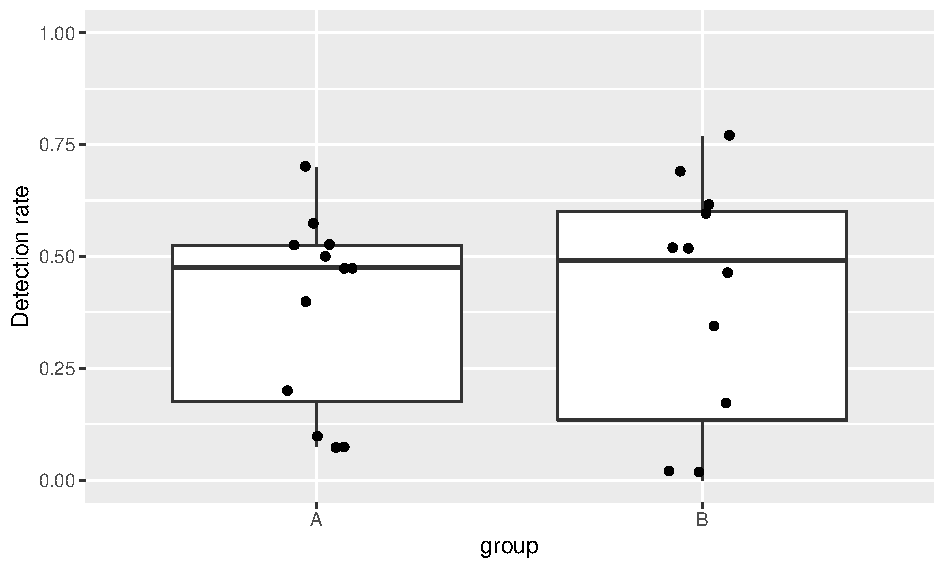
\includegraphics{thesis_files/figure-latex/pdetection-group-1.pdf}
\caption{\label{fig:pdetection-group}Boxplots of the distribution of detection rates for each line up, separated by group.}
\end{figure}

The overall detection rate is considered for each trend model in Fig. \ref{fig:pdetect-trend}.
The detection rates for the NW-SE trend model was less varied than the detection rates for the Three Cities and All Cities trends. Fig. \ref{fig:pdetection-group} shows the distribution using a boxplot. This shows the distributions of the rates do not overlap for NW-SE and Three Cities trends, the Three cities range was larger, but the median was much higher for the NW-SE trend. The All Cities trend model distribution overlaps with the NW-SE and All Cities trends.

\begin{Shaded}
\begin{Highlighting}[]
\NormalTok{plots }\OperatorTok\StringTok{ }\KeywordTok{ggplot}\NormalTok{(}\KeywordTok{aes}\NormalTok{(}\DataTypeTok{x =}\NormalTok{ trend, }\DataTypeTok{y =}\NormalTok{ pdetect, }\DataTypeTok{fill =}\NormalTok{ trend)) }\OperatorTok{+}\StringTok{ }
\StringTok{  }\KeywordTok{geom_boxplot}\NormalTok{() }\OperatorTok{+}\StringTok{ }
\StringTok{  }\KeywordTok{scale_fill_manual}\NormalTok{(}\DataTypeTok{values =}\NormalTok{ trend_colours) }\OperatorTok{+}
\StringTok{  }\KeywordTok{geom_jitter}\NormalTok{(}\DataTypeTok{width =} \FloatTok{0.1}\NormalTok{) }\OperatorTok{+}\StringTok{ }
\StringTok{  }\KeywordTok{guides}\NormalTok{(}\DataTypeTok{fill =} \OtherTok{FALSE}\NormalTok{) }\OperatorTok{+}
\StringTok{  }\KeywordTok{ylab}\NormalTok{(}\StringTok{"Detection rate"}\NormalTok{) }\OperatorTok{+}\StringTok{ }
\StringTok{  }\KeywordTok{ylim}\NormalTok{(}\KeywordTok{c}\NormalTok{(}\DecValTok{0}\NormalTok{,}\DecValTok{1}\NormalTok{)) }
\end{Highlighting}
\end{Shaded}

\begin{figure}
\centering
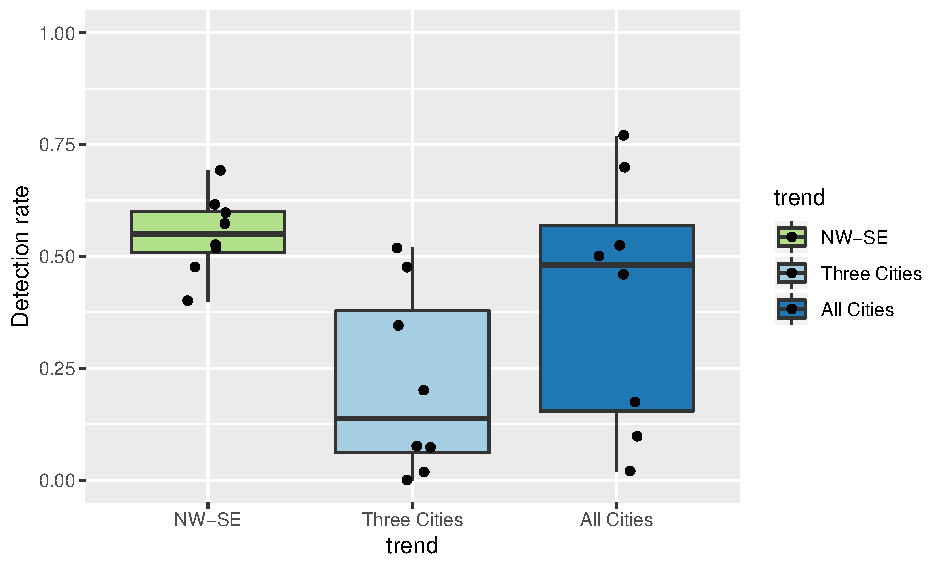
\includegraphics{thesis_files/figure-latex/pdetect-trend-1.pdf}
\caption{\label{fig:pdetect-trend}Boxplots of the distribution of detection rates for each line up, separated by trend model.}
\end{figure}

The boxplots in Fig. \ref{fig:pdetection-type} contrast the distribution of the detection rates for eah type of display.
The detection rates across the lineups was less varied for the hexagon display. There was a large difference in the medians for the types of displays.
Without considering the relationship for each lineup, the hexagon lineup display allowed the participants to achieve higher detection rates.

\begin{Shaded}
\begin{Highlighting}[]
\NormalTok{plots }\OperatorTok\StringTok{ }\KeywordTok{ggplot}\NormalTok{(}\KeywordTok{aes}\NormalTok{(}\DataTypeTok{x =}\NormalTok{ type, }\DataTypeTok{y =}\NormalTok{ pdetect, }\DataTypeTok{fill =}\NormalTok{ type)) }\OperatorTok{+}\StringTok{ }
\StringTok{  }\KeywordTok{geom_boxplot}\NormalTok{() }\OperatorTok{+}\StringTok{ }
\StringTok{  }\KeywordTok{geom_jitter}\NormalTok{(}\DataTypeTok{width =} \FloatTok{0.1}\NormalTok{) }\OperatorTok{+}
\StringTok{  }\KeywordTok{scale_fill_manual}\NormalTok{(}\DataTypeTok{values =}\NormalTok{ type_colours) }\OperatorTok{+}
\StringTok{  }\KeywordTok{guides}\NormalTok{(}\DataTypeTok{fill =} \OtherTok{FALSE}\NormalTok{) }\OperatorTok{+}
\StringTok{  }\KeywordTok{ylab}\NormalTok{(}\StringTok{"Detection rate"}\NormalTok{) }\OperatorTok{+}\StringTok{ }
\StringTok{  }\KeywordTok{ylim}\NormalTok{(}\KeywordTok{c}\NormalTok{(}\DecValTok{0}\NormalTok{,}\DecValTok{1}\NormalTok{))}
\end{Highlighting}
\end{Shaded}

\begin{figure}
\centering
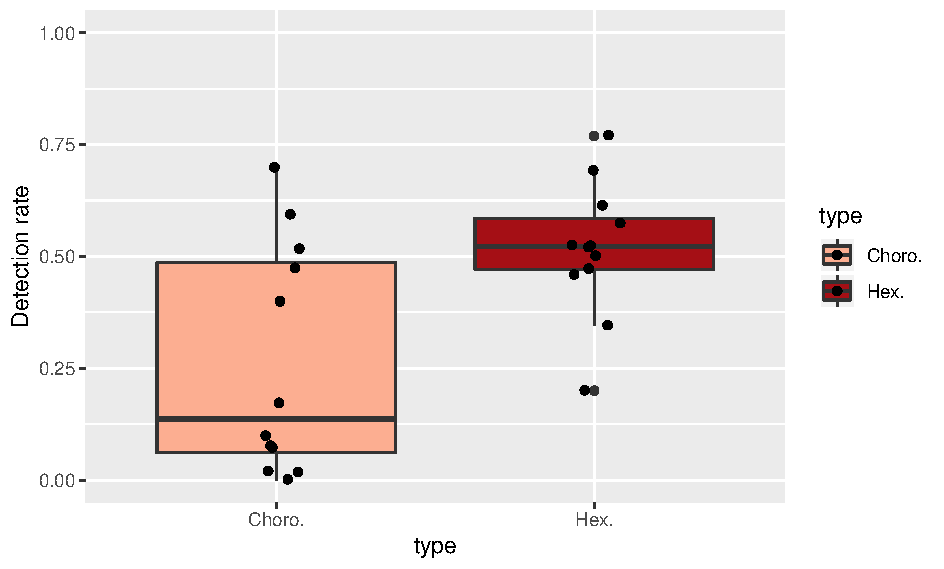
\includegraphics{thesis_files/figure-latex/pdetection-type-1.pdf}
\caption{\label{fig:pdetection-type}Boxplots of the distribution of detection rates for each line up, separated by type of display.}
\end{figure}

\hypertarget{lineups}{%
\section{Lineups}\label{lineups}}

Each lineup had twelve map displays, this gave participants the choice of any plot, and the choice to not provide a response. this non-reponse is indicated by 0.
The choices made by participants are displayed in Fig. \ref{fig:choices}. The height of each orange lollipop indiates the proportion of participants that selected the map display of real data, they represent the correct choices.
The green lollipops show the proportion of participants that selected the incorrect displays in each lineup.

The proportion of choices are also presented separately for each trend model in Table. \ref{tab:choice-nwse}, Table. \ref{tab:choice-three}, and Table. \ref{tab:choice-all}.
The correct map display in lineups with a North West to South East trend was chosen correctly with much greater frequency.
In the lineups of All Cities displays, participants were misled by the choropleth display, but not the hexagon display for all except (2).
All of Three Cities displays, except (4), were detected in the hexagon display. All except one lineup had at least one participant select the correct map in the lineup as shown in Fig. \ref{fig:choices}.

\begin{Shaded}
\begin{Highlighting}[]
\NormalTok{d }\OperatorTok\StringTok{ }
\StringTok{  }\KeywordTok{count}\NormalTok{(type, trend, choice, replicate, choice, detect_f) }\OperatorTok\StringTok{ }
\StringTok{  }\KeywordTok{group_by}\NormalTok{(type, trend, replicate) }\OperatorTok\StringTok{ }
\StringTok{  }\KeywordTok{mutate}\NormalTok{(}\DataTypeTok{prop =}\NormalTok{ n}\OperatorTok{/}\KeywordTok{sum}\NormalTok{(n)) }\OperatorTok\StringTok{ }
\StringTok{  }\KeywordTok{mutate}\NormalTok{(}\DataTypeTok{repl =} \KeywordTok{paste}\NormalTok{(}\StringTok{"Rep:"}\NormalTok{, replicate, }\StringTok{":}\CharTok{\textbackslash{}n}\StringTok{"}\NormalTok{, type,  }\DataTypeTok{sep =} \StringTok{""}\NormalTok{)) }\OperatorTok
\StringTok{  }\KeywordTok{mutate}\NormalTok{(}\DataTypeTok{bottom =} \DecValTok{0}\NormalTok{) }\OperatorTok\StringTok{ }
\StringTok{  }\KeywordTok{ggplot}\NormalTok{() }\OperatorTok{+}\StringTok{ }
\StringTok{  }\KeywordTok{geom_point}\NormalTok{(}\KeywordTok{aes}\NormalTok{(}\DataTypeTok{x =}\NormalTok{ choice, }\DataTypeTok{y =}\NormalTok{ prop, }\DataTypeTok{color =}\NormalTok{ detect_f), }\DataTypeTok{size =} \DecValTok{3}\NormalTok{) }\OperatorTok{+}\StringTok{ }
\StringTok{  }\KeywordTok{geom_segment}\NormalTok{(}\KeywordTok{aes}\NormalTok{(}\DataTypeTok{x =}\NormalTok{ choice, }\DataTypeTok{xend =}\NormalTok{ choice,}\DataTypeTok{y =}\NormalTok{ bottom, }\DataTypeTok{yend =}\NormalTok{ prop, }\DataTypeTok{colour =}\NormalTok{ detect_f), }\DataTypeTok{size =} \DecValTok{1}\NormalTok{) }\OperatorTok{+}
\StringTok{  }\KeywordTok{facet_grid}\NormalTok{(repl }\OperatorTok{~}\StringTok{ }\NormalTok{trend, }
    \DataTypeTok{drop =} \OtherTok{TRUE}\NormalTok{, }\DataTypeTok{as.table =} \OtherTok{TRUE}\NormalTok{, }\DataTypeTok{scales =} \StringTok{"free_y"}\NormalTok{) }\OperatorTok{+}
\StringTok{  }\KeywordTok{labs}\NormalTok{(}\DataTypeTok{x =} \StringTok{"Choice of plot in lineup"}\NormalTok{, }\DataTypeTok{y =} \StringTok{"Amount of choices"}\NormalTok{) }\OperatorTok{+}
\StringTok{  }\KeywordTok{scale_colour_manual}\NormalTok{(}\DataTypeTok{values =}\NormalTok{ detect_colours) }\OperatorTok{+}
\StringTok{  }\KeywordTok{scale_x_continuous}\NormalTok{(}\DataTypeTok{breaks =} \KeywordTok{seq}\NormalTok{(}\DataTypeTok{from =} \DecValTok{0}\NormalTok{, }\DataTypeTok{to =} \DecValTok{12}\NormalTok{)) }\OperatorTok{+}
\StringTok{  }\KeywordTok{scale_y_continuous}\NormalTok{(}\DataTypeTok{breaks =} \KeywordTok{seq}\NormalTok{(}\DataTypeTok{from =} \FloatTok{0.0}\NormalTok{, }\DataTypeTok{to =} \FloatTok{1.0}\NormalTok{, }\DataTypeTok{by =} \FloatTok{0.1}\NormalTok{)) }\OperatorTok{+}
\StringTok{  }\KeywordTok{theme}\NormalTok{(}\DataTypeTok{legend.position =} \StringTok{"bottom"}\NormalTok{) }\OperatorTok{+}\StringTok{ }
\StringTok{  }\KeywordTok{guides}\NormalTok{(}\DataTypeTok{colour =} \OtherTok{FALSE}\NormalTok{, }\DataTypeTok{fill =} \OtherTok{FALSE}\NormalTok{) }\OperatorTok{+}
\StringTok{  }\KeywordTok{theme}\NormalTok{(}\DataTypeTok{strip.text.y =} \KeywordTok{element_text}\NormalTok{(}\DataTypeTok{angle =} \DecValTok{0}\NormalTok{))}
\end{Highlighting}
\end{Shaded}

\begin{figure}
\centering
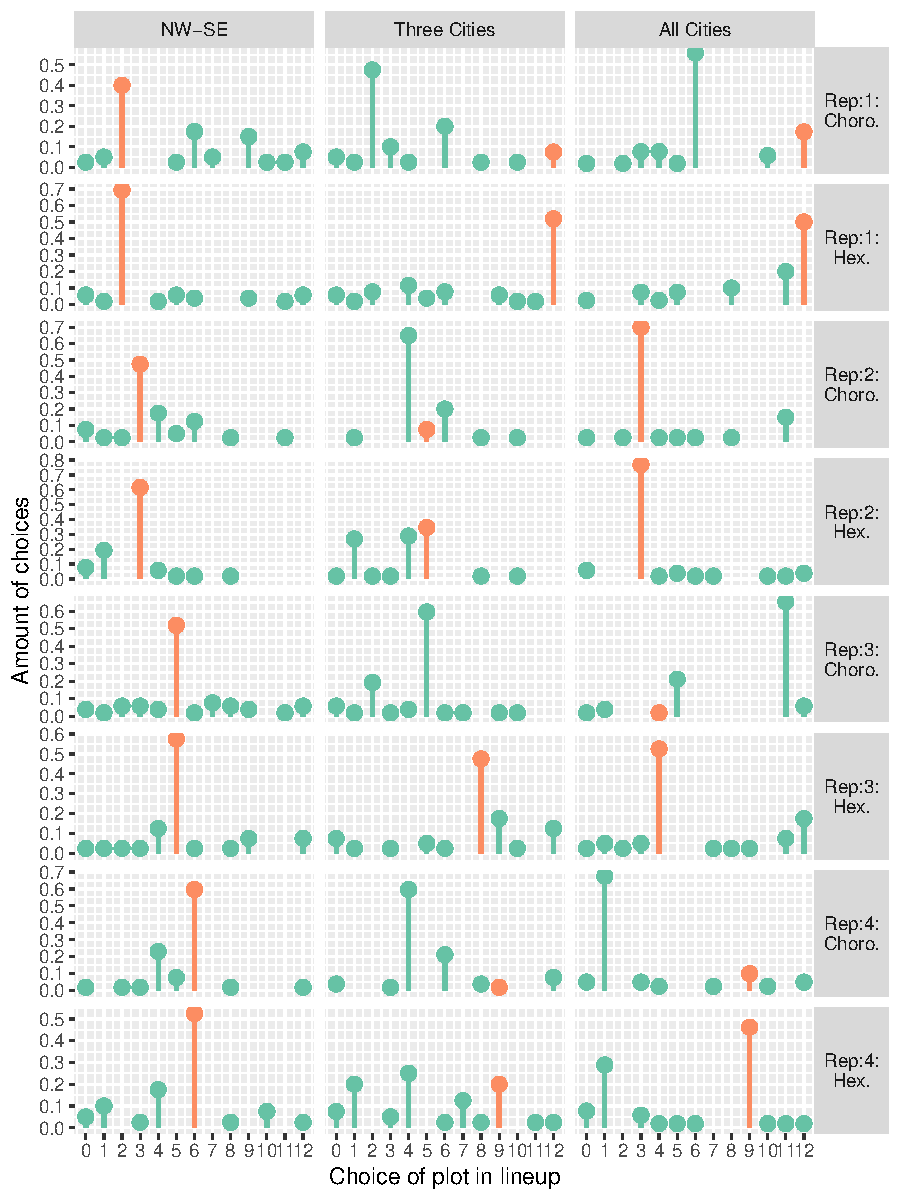
\includegraphics{thesis_files/figure-latex/choices-1.pdf}
\caption{\label{fig:choices}Pin plots of the propotion of choices made for each lineup location. Each facet is associated with one lineup, the height of the points show the proportion of the participants that made each choice when considering each lineup. The points coloured orange show the map which contained a trend model, these are the correct choices. The numbers differentiate the replicates of each trend model and type of map display. Participants were able to select 0 to indicate they did not want to choose a map.}
\end{figure}

\begin{Shaded}
\begin{Highlighting}[]
\NormalTok{choice_tabs <-}\StringTok{ }\NormalTok{d }\OperatorTok\StringTok{ }
\StringTok{  }\KeywordTok{count}\NormalTok{(trend, type, choice, replicate, choice, detect) }\OperatorTok\StringTok{ }
\StringTok{  }\KeywordTok{group_by}\NormalTok{(trend, type, replicate) }\OperatorTok\StringTok{ }
\StringTok{  }\KeywordTok{mutate}\NormalTok{(}\DataTypeTok{prop =} \KeywordTok{as.character}\NormalTok{(}\KeywordTok{round}\NormalTok{(n}\OperatorTok{/}\KeywordTok{sum}\NormalTok{(n), }\DecValTok{2}\NormalTok{))) }\OperatorTok\StringTok{ }
\StringTok{  }\KeywordTok{rowwise}\NormalTok{() }\OperatorTok\StringTok{ }
\StringTok{  }\KeywordTok{mutate}\NormalTok{(}\DataTypeTok{prop =} \KeywordTok{ifelse}\NormalTok{(}\KeywordTok{nchar}\NormalTok{(prop)}\OperatorTok{==}\DecValTok{3}\NormalTok{, }\KeywordTok{paste0}\NormalTok{(prop,}\DecValTok{0}\NormalTok{), prop)) }\OperatorTok\StringTok{ }
\StringTok{  }\KeywordTok{mutate}\NormalTok{(}\DataTypeTok{repl =} \KeywordTok{paste}\NormalTok{(}\StringTok{"Rep:"}\NormalTok{, replicate, }\StringTok{":}\CharTok{\textbackslash{}n}\StringTok{"}\NormalTok{, type,  }\DataTypeTok{sep =} \StringTok{""}\NormalTok{)) }\OperatorTok
\StringTok{  }\KeywordTok{mutate}\NormalTok{(}\DataTypeTok{bottom =} \DecValTok{0}\NormalTok{) }\OperatorTok\StringTok{ }
\StringTok{  }\KeywordTok{select}\NormalTok{(}\DataTypeTok{Trend =}\NormalTok{ trend, }\DataTypeTok{Rep =}\NormalTok{ replicate, }\DataTypeTok{Type =}\NormalTok{ type, prop, choice) }\OperatorTok\StringTok{ }
\StringTok{  }\KeywordTok{spread}\NormalTok{(choice, prop, }\DataTypeTok{fill =} \StringTok{"0.00"}\NormalTok{) }\OperatorTok\StringTok{ }
\StringTok{  }\KeywordTok{nest}\NormalTok{(}\DataTypeTok{data =} \KeywordTok{c}\NormalTok{(Rep, Type, }\StringTok{`}\DataTypeTok{0}\StringTok{`}\NormalTok{, }\StringTok{`}\DataTypeTok{1}\StringTok{`}\NormalTok{, }\StringTok{`}\DataTypeTok{2}\StringTok{`}\NormalTok{, }\StringTok{`}\DataTypeTok{3}\StringTok{`}\NormalTok{, }\StringTok{`}\DataTypeTok{4}\StringTok{`}\NormalTok{, }\StringTok{`}\DataTypeTok{5}\StringTok{`}\NormalTok{, }\StringTok{`}\DataTypeTok{6}\StringTok{`}\NormalTok{, }\StringTok{`}\DataTypeTok{7}\StringTok{`}\NormalTok{, }\StringTok{`}\DataTypeTok{8}\StringTok{`}\NormalTok{, }\StringTok{`}\DataTypeTok{9}\StringTok{`}\NormalTok{, }
    \StringTok{`}\DataTypeTok{10}\StringTok{`}\NormalTok{, }\StringTok{`}\DataTypeTok{11}\StringTok{`}\NormalTok{, }\StringTok{`}\DataTypeTok{12}\StringTok{`}\NormalTok{))}
\end{Highlighting}
\end{Shaded}

\begin{table}

\caption{\label{tab:choice-nwse}The proportion of participants who selected each of the twelve map choices in each lineup for NW-SE displays.}
\centering
\begin{tabular}[t]{rrrrrrrrrrrrrrr}
\toprule
Rep & Type & 0 & 1 & 2 & 3 & 4 & 5 & 6 & 7 & 8 & 9 & 10 & 11 & 12\\
\midrule
 & Choro. & 0.00 & 0.05 & 0.41 & 0.00 & 0.00 & 0.03 & 0.18 & 0.05 & 0.00 & 0.15 & 0.03 & 0.03 & 0.08\\
\cmidrule{2-15}
\multirow{-2}{*}{\raggedleft\arraybackslash 1} & Hex. & 0.04 & 0.02 & 0.71 & 0.00 & 0.02 & 0.06 & 0.04 & 0.00 & 0.00 & 0.04 & 0.00 & 0.02 & 0.06\\
\cmidrule{1-15}
 & Choro. & 0.05 & 0.03 & 0.03 & 0.49 & 0.18 & 0.05 & 0.13 & 0.00 & 0.03 & 0.00 & 0.00 & 0.03 & 0.00\\
\cmidrule{2-15}
\multirow{-2}{*}{\raggedleft\arraybackslash 2} & Hex. & 0.06 & 0.20 & 0.00 & 0.63 & 0.06 & 0.02 & 0.02 & 0.00 & 0.02 & 0.00 & 0.00 & 0.00 & 0.00\\
\cmidrule{1-15}
 & Choro. & 0.02 & 0.02 & 0.06 & 0.06 & 0.04 & 0.53 & 0.02 & 0.08 & 0.06 & 0.04 & 0.00 & 0.02 & 0.06\\
\cmidrule{2-15}
\multirow{-2}{*}{\raggedleft\arraybackslash 3} & Hex. & 0.00 & 0.03 & 0.03 & 0.03 & 0.13 & 0.59 & 0.03 & 0.00 & 0.03 & 0.08 & 0.00 & 0.00 & 0.08\\
\cmidrule{1-15}
 & Choro. & 0.00 & 0.00 & 0.02 & 0.02 & 0.24 & 0.08 & 0.61 & 0.00 & 0.02 & 0.00 & 0.00 & 0.00 & 0.02\\
\cmidrule{2-15}
\multirow{-2}{*}{\raggedleft\arraybackslash 4} & Hex. & 0.03 & 0.10 & 0.00 & 0.03 & 0.18 & 0.00 & 0.54 & 0.00 & 0.03 & 0.00 & 0.08 & 0.00 & 0.03\\
\bottomrule
\end{tabular}
\end{table}

\begin{table}

\caption{\label{tab:choice-three}The proportion of participants who selected each of the twelve map choices in each lineup for Three Cities displays.}
\centering
\begin{tabular}[t]{rrrrrrrrrrrrrrr}
\toprule
Rep & Type & 0 & 1 & 2 & 3 & 4 & 5 & 6 & 7 & 8 & 9 & 10 & 11 & 12\\
\midrule
 & Choro. & 0.05 & 0.03 & 0.49 & 0.08 & 0.03 & 0.00 & 0.21 & 0.00 & 0.03 & 0.00 & 0.03 & 0.00 & 0.08\\
\cmidrule{2-15}
\multirow{-2}{*}{\raggedleft\arraybackslash 1} & Hex. & 0.04 & 0.02 & 0.08 & 0.00 & 0.12 & 0.04 & 0.08 & 0.00 & 0.00 & 0.06 & 0.02 & 0.02 & 0.53\\
\cmidrule{1-15}
 & Choro. & 0.00 & 0.03 & 0.00 & 0.00 & 0.67 & 0.08 & 0.18 & 0.00 & 0.03 & 0.00 & 0.03 & 0.00 & 0.00\\
\cmidrule{2-15}
\multirow{-2}{*}{\raggedleft\arraybackslash 2} & Hex. & 0.00 & 0.27 & 0.02 & 0.02 & 0.29 & 0.35 & 0.00 & 0.00 & 0.02 & 0.00 & 0.02 & 0.00 & 0.00\\
\cmidrule{1-15}
 & Choro. & 0.04 & 0.02 & 0.20 & 0.02 & 0.04 & 0.61 & 0.02 & 0.02 & 0.00 & 0.02 & 0.02 & 0.00 & 0.00\\
\cmidrule{2-15}
\multirow{-2}{*}{\raggedleft\arraybackslash 3} & Hex. & 0.05 & 0.03 & 0.00 & 0.03 & 0.00 & 0.05 & 0.03 & 0.00 & 0.49 & 0.18 & 0.03 & 0.00 & 0.13\\
\cmidrule{1-15}
 & Choro. & 0.04 & 0.00 & 0.00 & 0.02 & 0.59 & 0.00 & 0.22 & 0.00 & 0.04 & 0.02 & 0.00 & 0.00 & 0.08\\
\cmidrule{2-15}
\multirow{-2}{*}{\raggedleft\arraybackslash 4} & Hex. & 0.05 & 0.21 & 0.00 & 0.05 & 0.26 & 0.00 & 0.03 & 0.13 & 0.03 & 0.21 & 0.00 & 0.03 & 0.03\\
\bottomrule
\end{tabular}
\end{table}

\begin{table}

\caption{\label{tab:choice-all}The proportion of participants who selected each of the twelve map choices in each lineup for All Cities displays.}
\centering
\begin{tabular}[t]{rrrrrrrrrrrrrrr}
\toprule
Rep & Type & 0 & 1 & 2 & 3 & 4 & 5 & 6 & 7 & 8 & 9 & 10 & 11 & 12\\
\midrule
 & Choro. & 0.00 & 0.00 & 0.02 & 0.08 & 0.08 & 0.02 & 0.57 & 0.00 & 0.00 & 0.00 & 0.06 & 0.00 & 0.18\\
\cmidrule{2-15}
\multirow{-2}{*}{\raggedleft\arraybackslash 1} & Hex. & 0.03 & 0.00 & 0.00 & 0.05 & 0.03 & 0.08 & 0.00 & 0.00 & 0.10 & 0.00 & 0.00 & 0.21 & 0.51\\
\cmidrule{1-15}
 & Choro. & 0.00 & 0.00 & 0.03 & 0.72 & 0.03 & 0.03 & 0.03 & 0.00 & 0.03 & 0.00 & 0.00 & 0.15 & 0.00\\
\cmidrule{2-15}
\multirow{-2}{*}{\raggedleft\arraybackslash 2} & Hex. & 0.04 & 0.00 & 0.00 & 0.78 & 0.02 & 0.04 & 0.02 & 0.02 & 0.00 & 0.00 & 0.02 & 0.02 & 0.04\\
\cmidrule{1-15}
 & Choro. & 0.00 & 0.04 & 0.00 & 0.00 & 0.02 & 0.22 & 0.00 & 0.00 & 0.00 & 0.00 & 0.00 & 0.67 & 0.06\\
\cmidrule{2-15}
\multirow{-2}{*}{\raggedleft\arraybackslash 3} & Hex. & 0.00 & 0.05 & 0.03 & 0.05 & 0.54 & 0.00 & 0.00 & 0.03 & 0.03 & 0.03 & 0.00 & 0.08 & 0.18\\
\cmidrule{1-15}
 & Choro. & 0.03 & 0.69 & 0.00 & 0.05 & 0.03 & 0.00 & 0.00 & 0.03 & 0.00 & 0.10 & 0.03 & 0.00 & 0.05\\
\cmidrule{2-15}
\multirow{-2}{*}{\raggedleft\arraybackslash 4} & Hex. & 0.06 & 0.29 & 0.00 & 0.06 & 0.02 & 0.02 & 0.02 & 0.00 & 0.00 & 0.47 & 0.02 & 0.02 & 0.02\\
\bottomrule
\end{tabular}
\end{table}

Lineups were created using the Australian Statistical Areas at Level 3.

\hypertarget{all-cities}{%
\section{All Cities}\label{all-cities}}

\hypertarget{replicate-1}{%
\subsection{Replicate 1}\label{replicate-1}}

\begin{figure}[H]
\centering
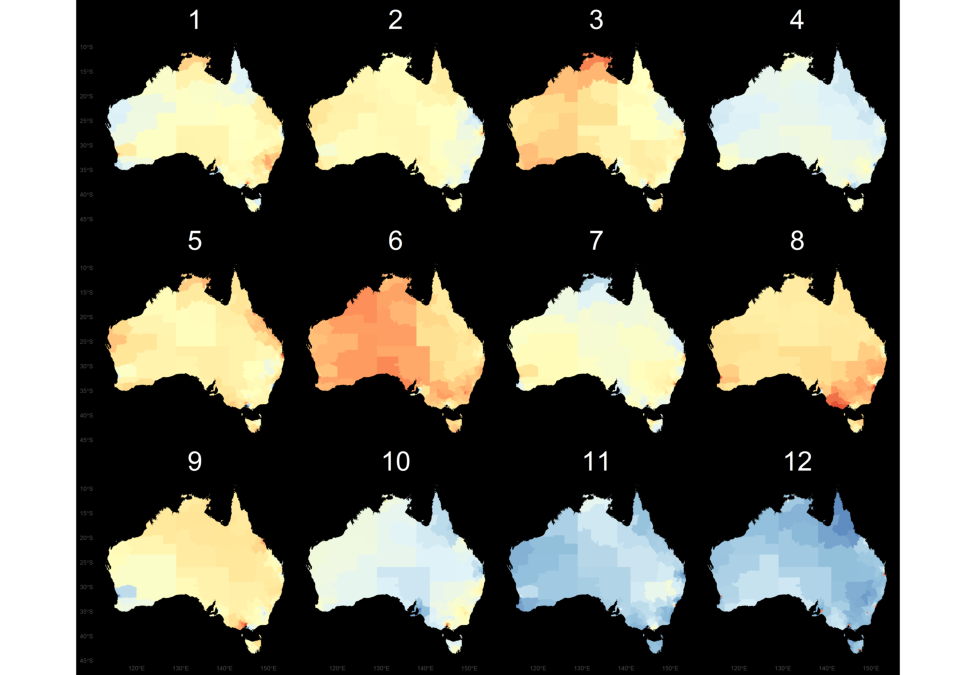
\includegraphics[height=8cm]{lineups/cities-geo12-1.pdf}
\caption{\label{fig:cities-geo12}A choropleth map lineup, location 12 contains a distribution that affects all capital cities.}
\end{figure}

\begin{figure}[H]
\centering
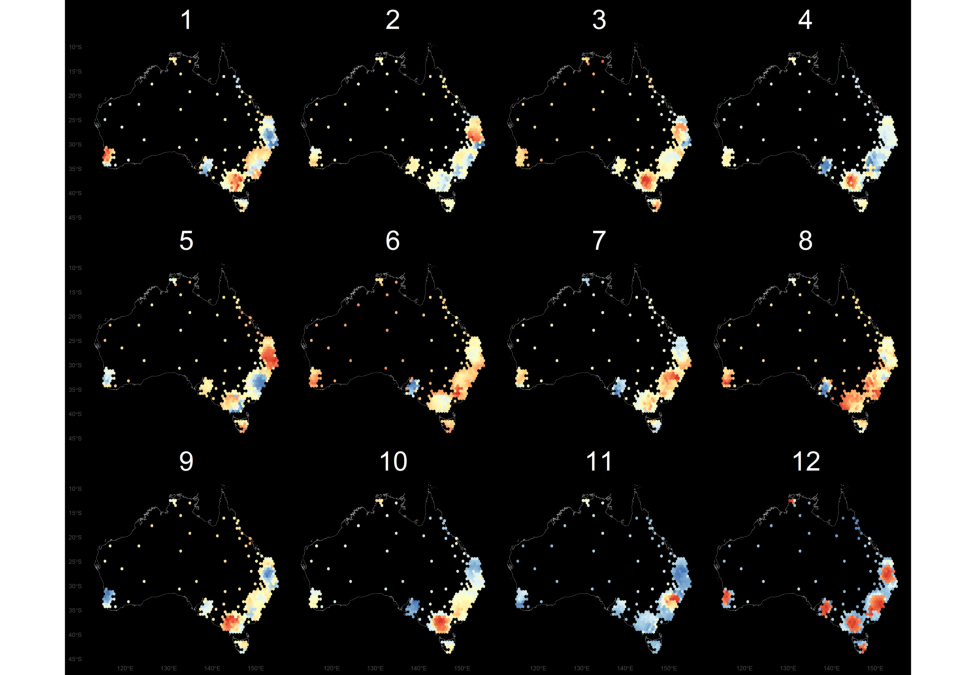
\includegraphics[height=8cm]{lineups/cities-hex12-1.pdf}
\caption{\label{fig:cities-hex12}A hxagon tile map lineup, location 12 contains a distribution that affects all capital cities.}
\end{figure}

\hypertarget{replicate-2}{%
\subsection{Replicate 2}\label{replicate-2}}

\begin{figure}[H]
\centering
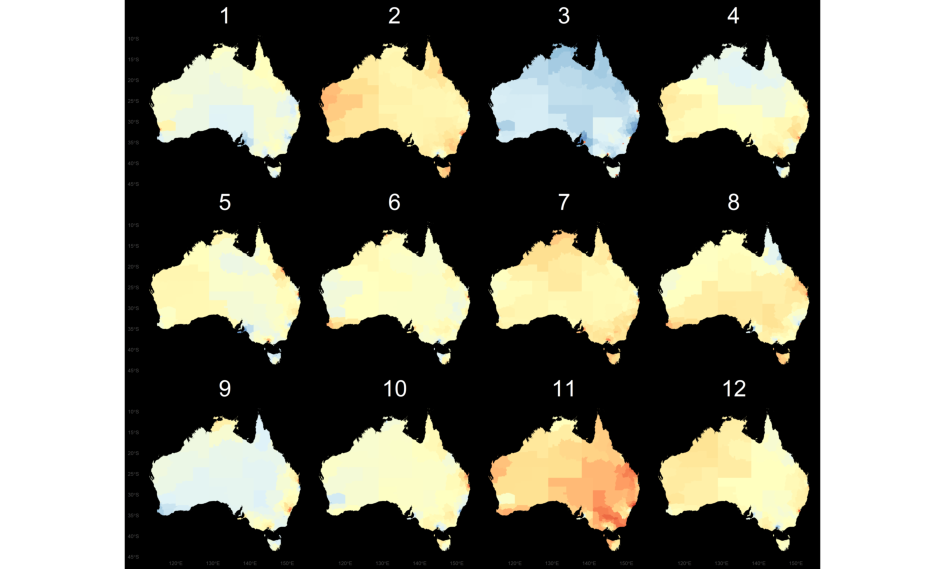
\includegraphics[height=8cm]{lineups/cities-geo3-1.pdf}
\caption{\label{fig:cities-geo3}A choropleth map lineup, location 3 contains a distribution that affects all capital cities.}
\end{figure}

\begin{figure}[H]
\centering
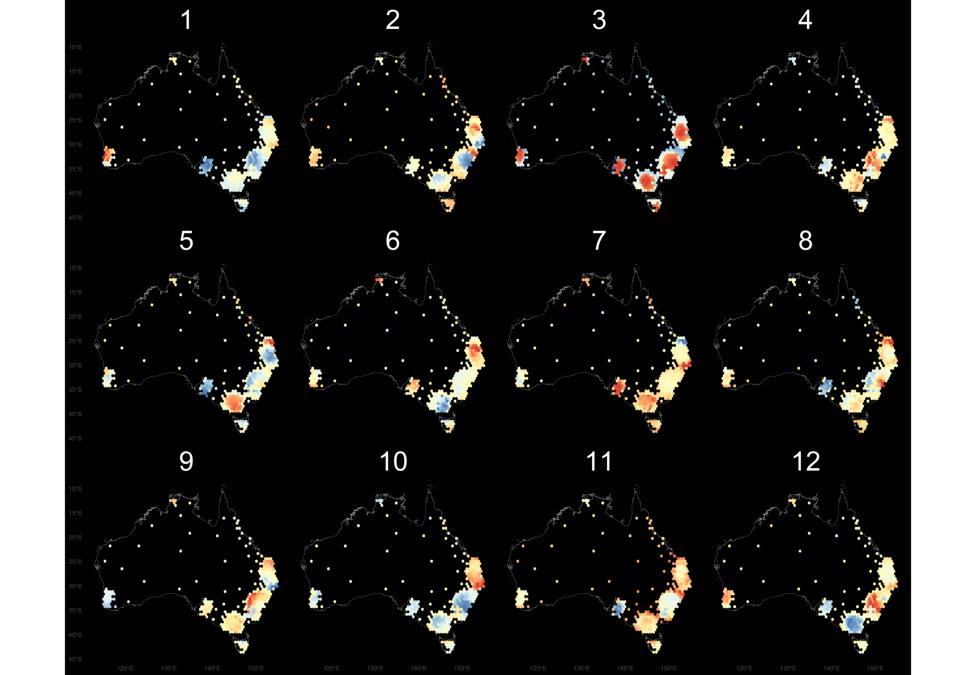
\includegraphics[height=8cm]{lineups/cities-hex3-1.pdf}
\caption{\label{fig:cities-hex3}A hxagon tile map lineup, location 3 contains a distribution that affects all capital cities.}
\end{figure}

\hypertarget{replicate-3}{%
\subsection{Replicate 3}\label{replicate-3}}

\begin{figure}[H]
\centering
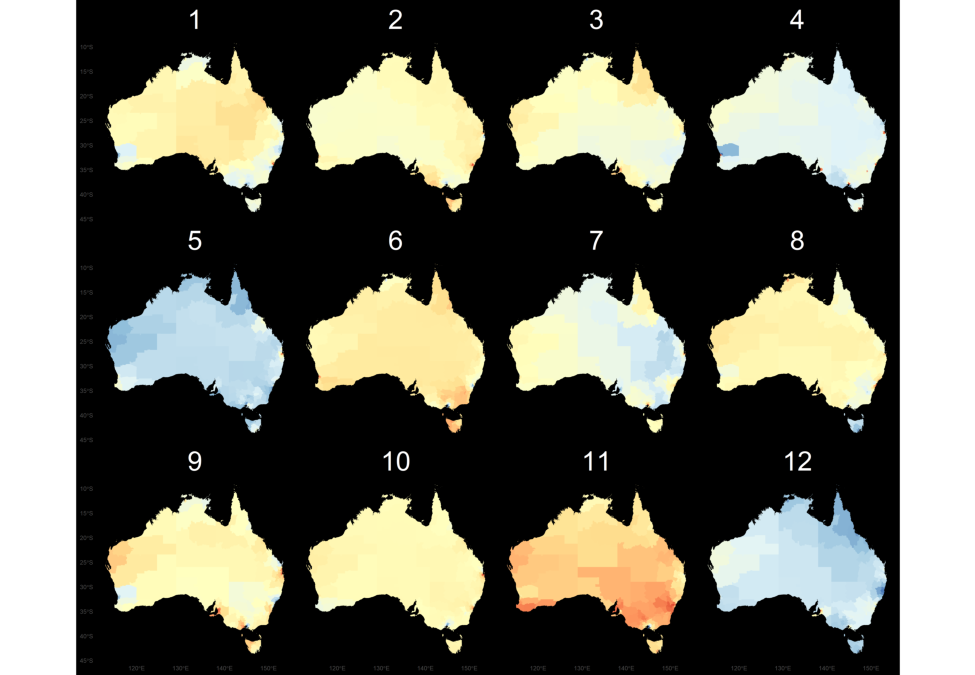
\includegraphics[height=8cm]{lineups/cities-geo4-1.pdf}
\caption{\label{fig:cities-geo4}A choropleth map lineup, location 4 contains a distribution that affects all capital cities.}
\end{figure}

\begin{figure}[H]
\centering
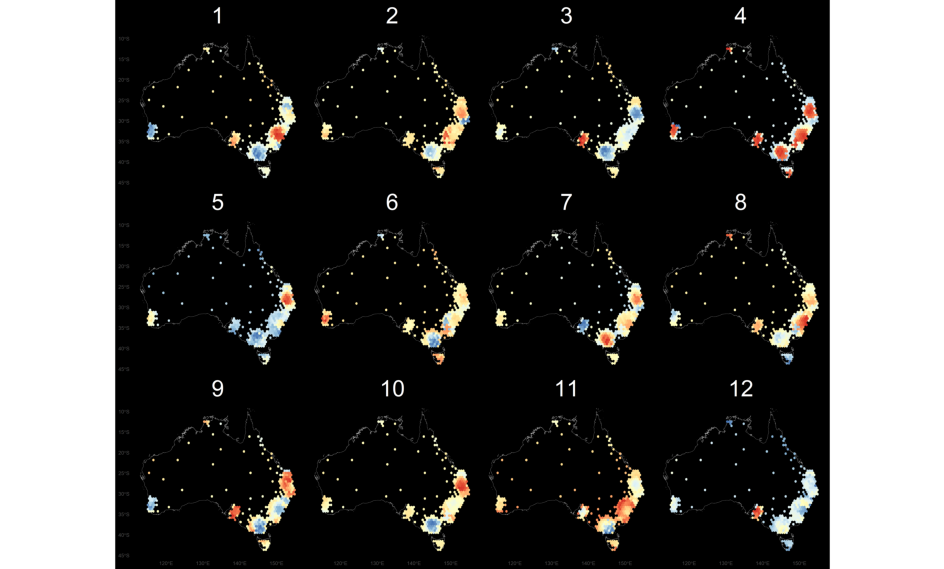
\includegraphics[height=8cm]{lineups/cities-hex4-1.pdf}
\caption{\label{fig:cities-hex4}A hxagon tile map lineup, location 4 contains a distribution that affects all capital cities.}
\end{figure}

\hypertarget{replicate-4}{%
\subsection{Replicate 4}\label{replicate-4}}

\begin{figure}[H]
\centering
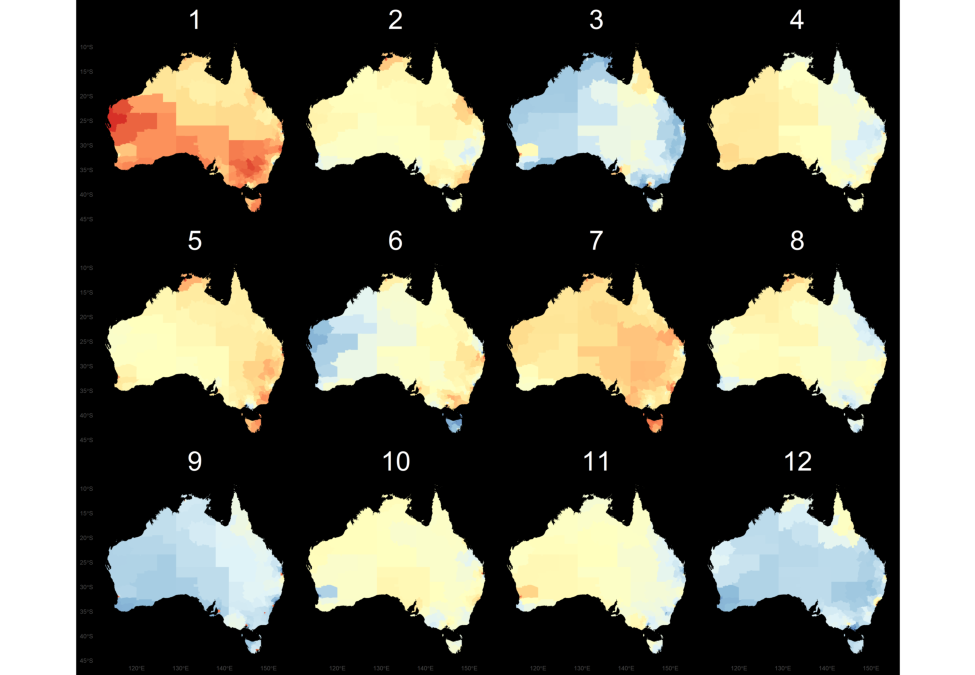
\includegraphics[height=8cm]{lineups/cities-geo9-1.pdf}
\caption{\label{fig:cities-geo9}A choropleth map lineup, location 9 contains a distribution that affects all capital cities.}
\end{figure}

\begin{figure}[H]
\centering
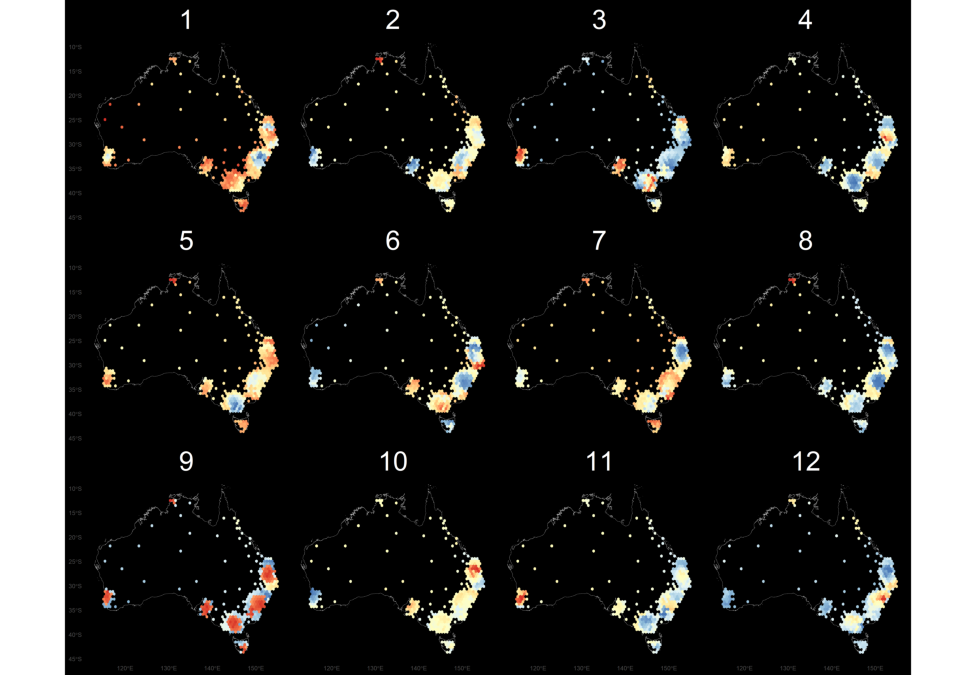
\includegraphics[height=8cm]{lineups/cities-hex9-1.pdf}
\caption{\label{fig:cities-hex9}A hxagon tile map lineup, location 9 contains a distribution that affects all capital cities.}
\end{figure}

\newpage

\hypertarget{three-cities}{%
\section{Three Cities}\label{three-cities}}

\hypertarget{replicate-1-1}{%
\subsection{Replicate 1}\label{replicate-1-1}}

\begin{figure}[H]
\centering
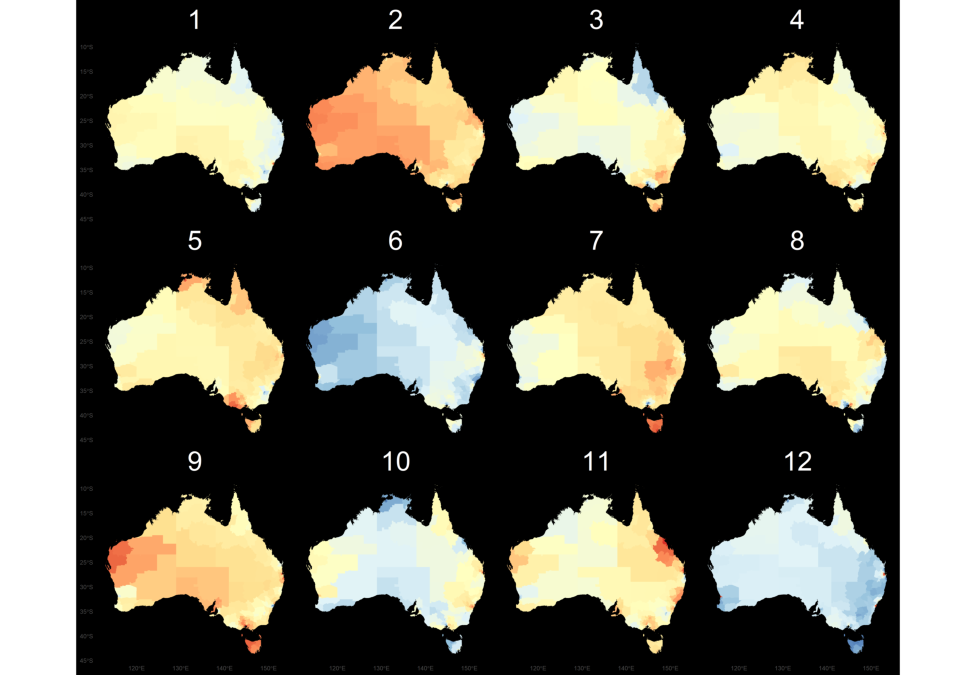
\includegraphics[height=8cm]{lineups/three-geo12-1.pdf}
\caption{\label{fig:three-geo12}A choropleth map lineup, location 12 contains a distribution that affects three of the Australian capital cities.}
\end{figure}

\begin{figure}[H]
\centering
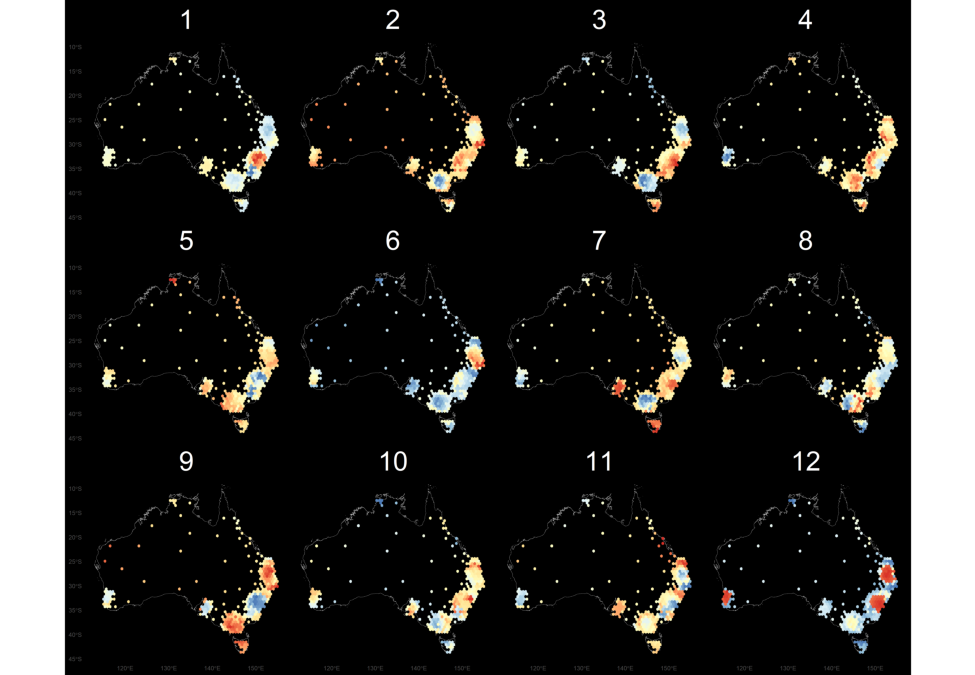
\includegraphics[height=8cm]{lineups/three-hex12-1.pdf}
\caption{\label{fig:three-hex12}A hxagon tile map lineup, location 12 contains a distribution that affects three of the Australian capital cities.}
\end{figure}

\hypertarget{replicate-2-1}{%
\subsection{Replicate 2}\label{replicate-2-1}}

\begin{figure}[H]
\centering
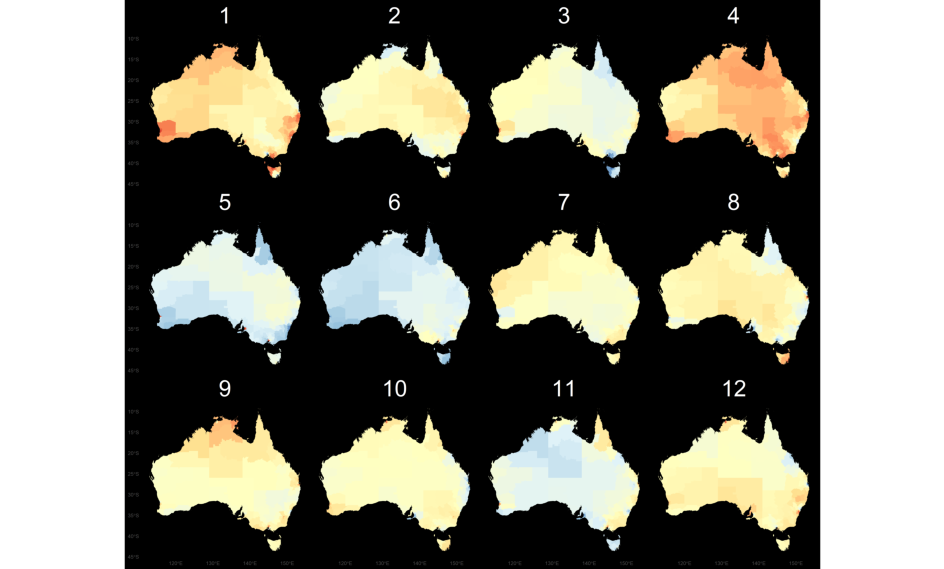
\includegraphics[height=8cm]{lineups/three-geo5-1.pdf}
\caption{\label{fig:three-geo5}A choropleth map lineup, location 3 contains a distribution that affects three of the Australian capital cities.}
\end{figure}

\begin{figure}[H]
\centering
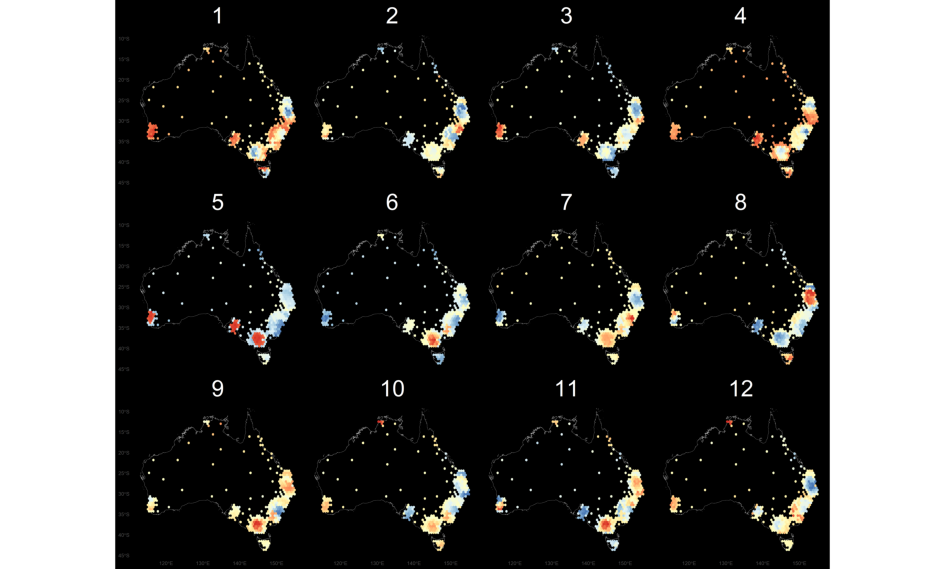
\includegraphics[height=8cm]{lineups/three-hex5-1.pdf}
\caption{\label{fig:three-hex5}A hxagon tile map lineup, location 3 contains a distribution that affects three of the Australian capital cities.}
\end{figure}

\hypertarget{replicate-3-1}{%
\subsection{Replicate 3}\label{replicate-3-1}}

\begin{figure}[H]
\centering
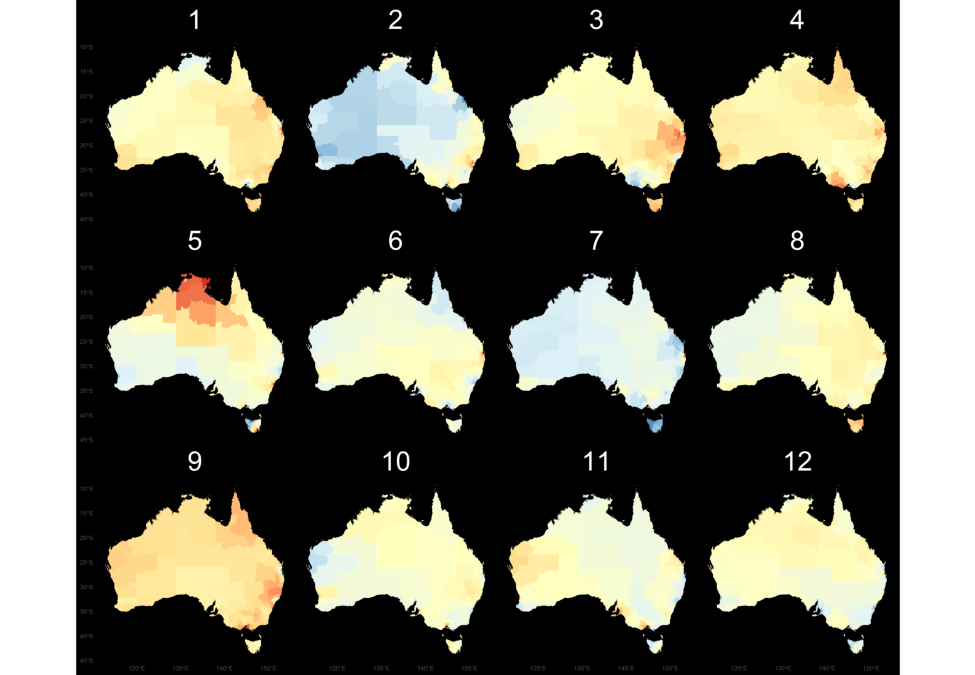
\includegraphics[height=8cm]{lineups/three-geo8-1.pdf}
\caption{\label{fig:three-geo8}A choropleth map lineup, location 4 contains a distribution that affects three of the Australian capital cities.}
\end{figure}

\begin{figure}[H]
\centering
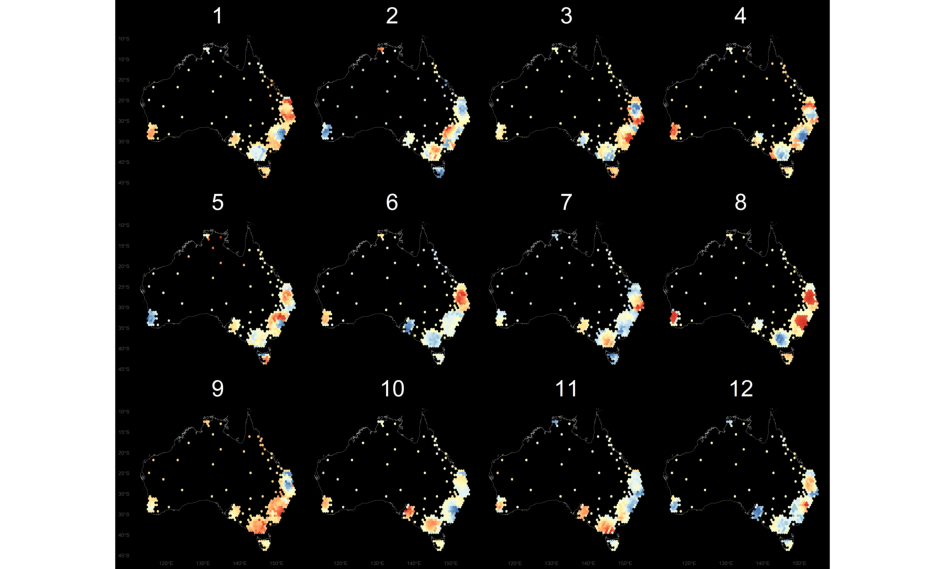
\includegraphics[height=8cm]{lineups/three-hex8-1.pdf}
\caption{\label{fig:three-hex8}A hxagon tile map lineup, location 4 contains a distribution that affects three of the Australian capital cities.}
\end{figure}

\hypertarget{replicate-4-1}{%
\subsection{Replicate 4}\label{replicate-4-1}}

\begin{figure}[H]
\centering
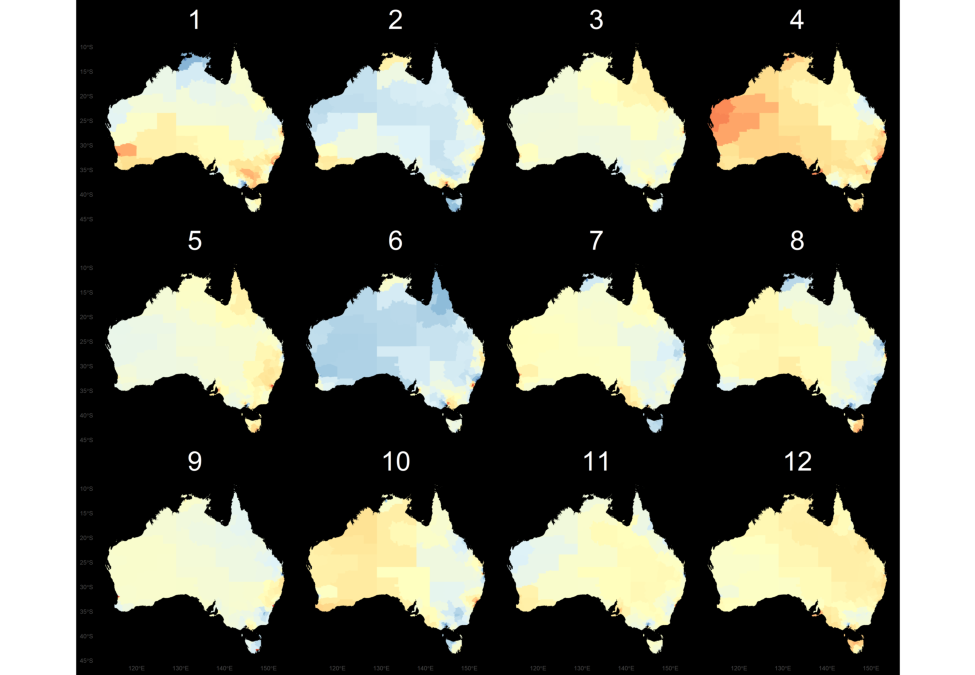
\includegraphics[height=8cm]{lineups/three-geo9-1.pdf}
\caption{\label{fig:three-geo9}A choropleth map lineup, location 9 contains a distribution that affects three of the Australian capital cities.}
\end{figure}

\begin{figure}[H]
\centering
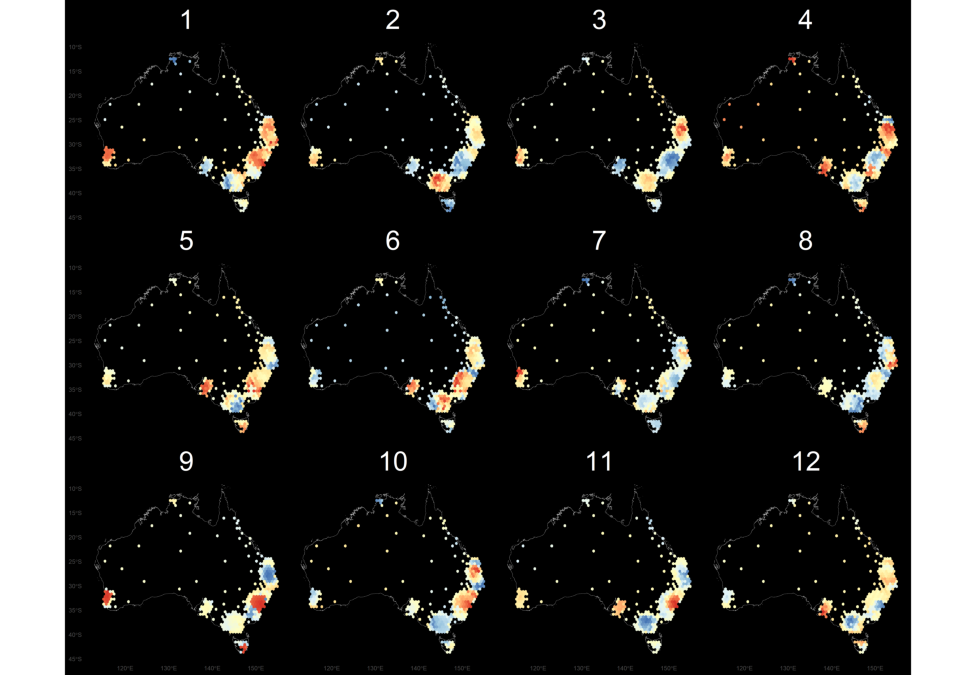
\includegraphics[height=8cm]{lineups/three-hex9-1.pdf}
\caption{\label{fig:three-hex9}A hxagon tile map lineup, location 9 contains a distribution that affects three of the Australian capital cities.}
\end{figure}

\hypertarget{north-west-to-south-east}{%
\section{North West to South East}\label{north-west-to-south-east}}

\hypertarget{replicate-1-2}{%
\subsection{Replicate 1}\label{replicate-1-2}}

\begin{figure}[H]
\centering
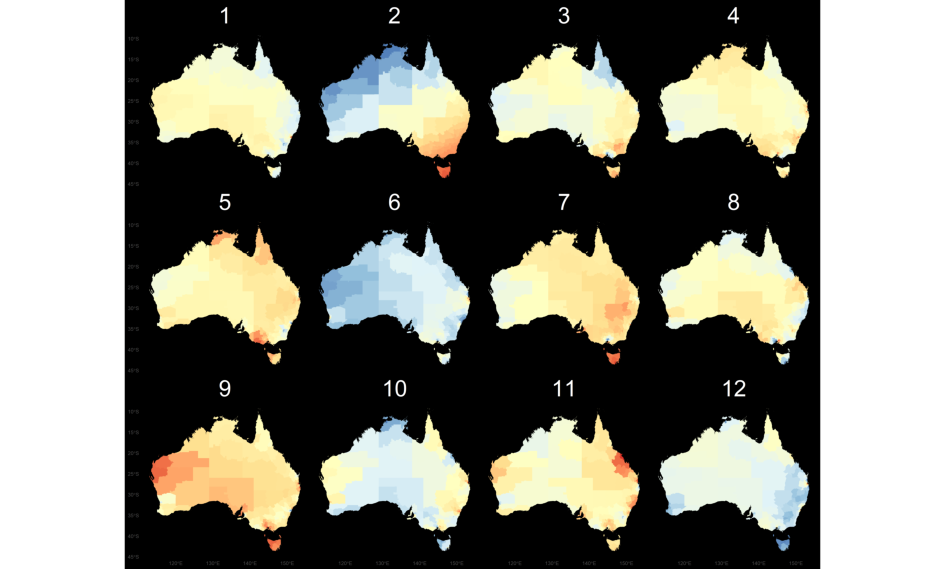
\includegraphics[height=8cm]{lineups/nwse-geo2-1.pdf}
\caption{\label{fig:nwse-geo2}A choropleth map lineup, location 12 contains a distribution that affects all capital nwse.}
\end{figure}

\begin{figure}[H]
\centering
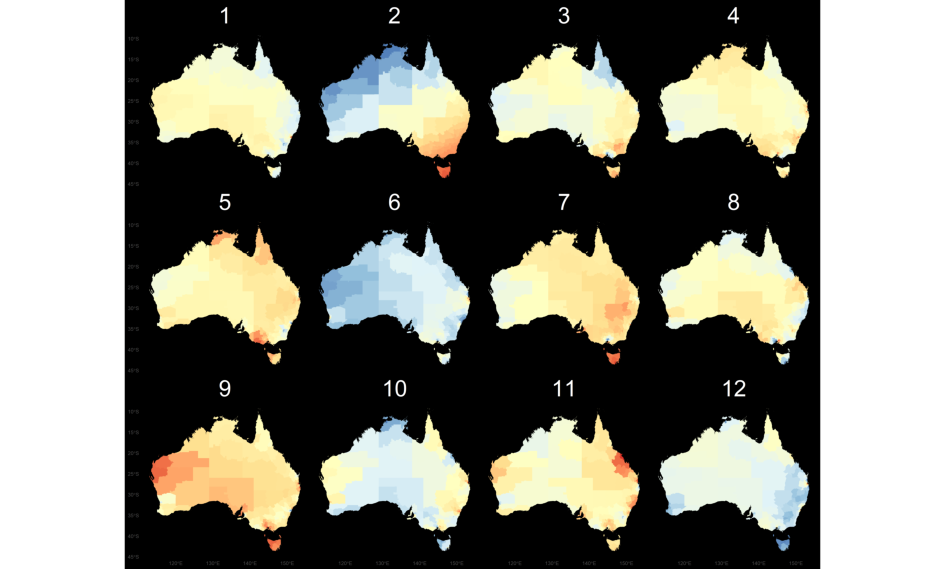
\includegraphics[height=8cm]{lineups/nwse-hex2-1.pdf}
\caption{\label{fig:nwse-hex2}A hxagon tile map lineup, location 12 contains a distribution that affects all capital nwse.}
\end{figure}

\hypertarget{replicate-2-2}{%
\subsection{Replicate 2}\label{replicate-2-2}}

\begin{figure}[H]
\centering
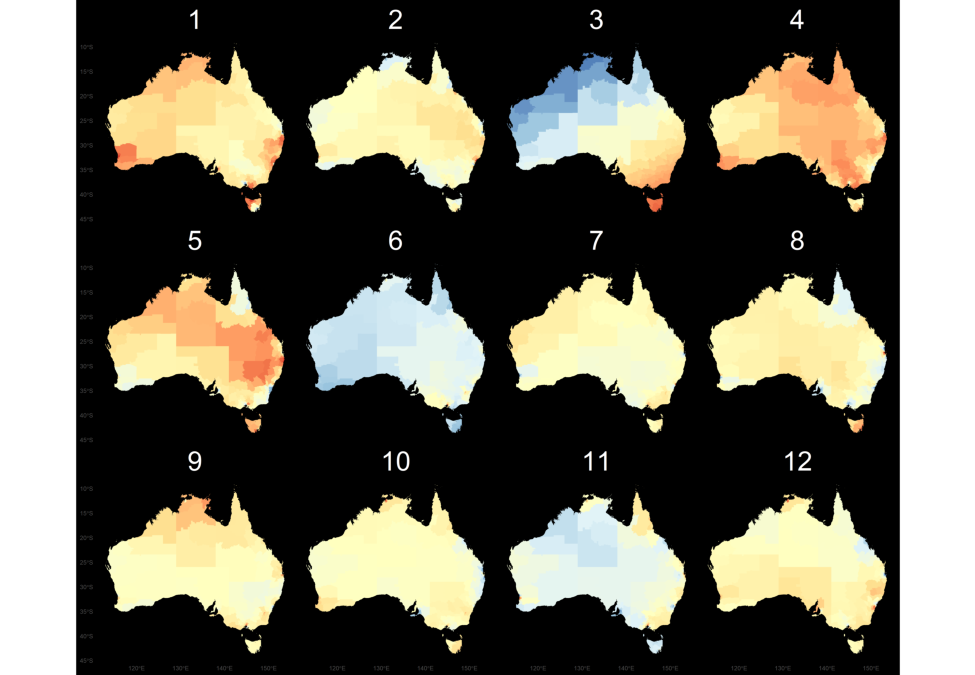
\includegraphics[height=8cm]{lineups/nwse-geo3-1.pdf}
\caption{\label{fig:nwse-geo3}A choropleth map lineup, location 3 contains a distribution that affects all capital nwse.}
\end{figure}

\begin{figure}[H]
\centering
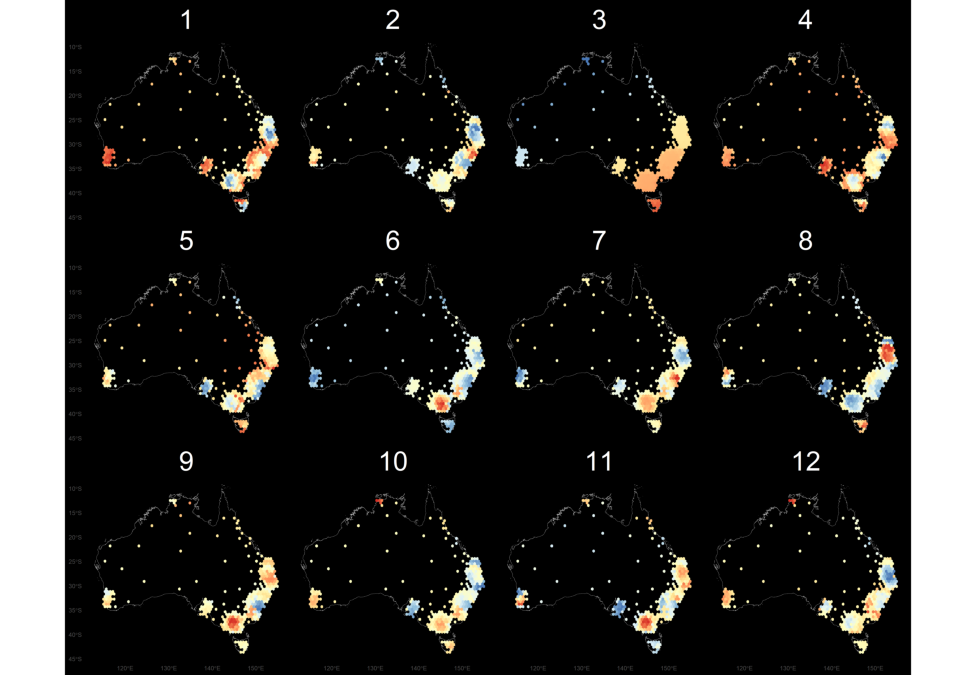
\includegraphics[height=8cm]{lineups/nwse-hex3-1.pdf}
\caption{\label{fig:nwse-hex3}A hxagon tile map lineup, location 3 contains a distribution that affects all capital nwse.}
\end{figure}

\hypertarget{replicate-3-2}{%
\subsection{Replicate 3}\label{replicate-3-2}}

\begin{figure}[H]
\centering
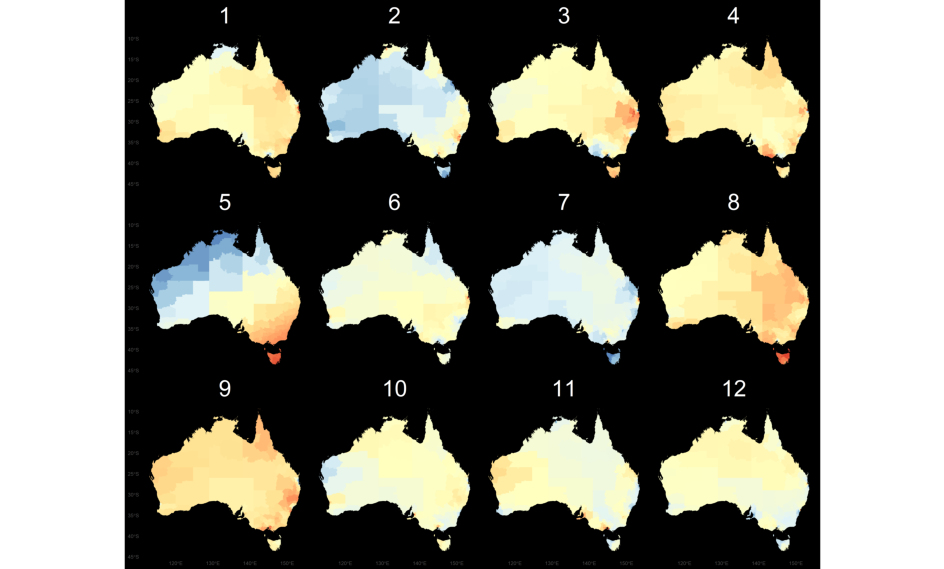
\includegraphics[height=8cm]{lineups/nwse-geo5-1.pdf}
\caption{\label{fig:nwse-geo5}A choropleth map lineup, location 4 contains a distribution that affects all capital nwse.}
\end{figure}

\begin{figure}[H]
\centering
\includegraphics[height=8cm]{lineups/nwse-hex5-1.pdf}
\caption{\label{fig:nwse-hex5}A hxagon tile map lineup, location 4 contains a distribution that affects all capital nwse.}
\end{figure}

\hypertarget{replicate-4-2}{%
\subsection{Replicate 4}\label{replicate-4-2}}

\begin{figure}[H]
\centering
\includegraphics[height=8cm]{lineups/nwse-geo6-1.pdf}
\caption{\label{fig:nwse-geo6}A choropleth map lineup, location 9 contains a distribution that affects all capital nwse.}
\end{figure}

\begin{figure}[H]
\centering
\includegraphics[height=8cm]{lineups/nwse-hex6-1.pdf}
\caption{\label{fig:nwse-hex6}A hxagon tile map lineup, location 9 contains a distribution that affects all capital nwse.}
\end{figure}

\hypertarget{experiment-survey-procedure}{%
\chapter{Experiment survey procedure}\label{experiment-survey-procedure}}

Participants were recruited via advertising on the Figure Eight crowdsource platform.
Choosing the task from the list directed all potential participants to the page of instructions.
This page contained written instructions and is shown in Fig. \ref{fig:instruct}.

\begin{figure}[H]
\centering
\includegraphics[height=16cm]{figures/fig8_instruct.png}
\caption{\label{fig:instruct}The training lineups of choropleth maps.}
\end{figure}

\hypertarget{training}{%
\section{Training}\label{training}}

The participants were trained using three displays. There were relatively simple lineups, they are displayed in Fig. \ref{fig:training1} and Fig. \ref{fig:training2}.

\begin{figure}[H]
\centering
\includegraphics[width=16cm]{figures/fig8_training1.png}
\caption{\label{fig:training1}The training lineups of choropleth maps.}
\end{figure}

\begin{figure}[H]
\centering
\includegraphics[width=16cm]{figures/fig8_training2.png}
\caption{\label{fig:training2}The training lineups of hexagon tile maps.}
\end{figure}

\hypertarget{survey-application}{%
\section{Survey application}\label{survey-application}}

The survey application was a \texttt{shinydashboard} we application, hosted on a website external to the Figure-Eight platform. The link to the survey was located at the bottom of the instructions and training page. Only participants who had read all of the instructions and seen the example image sets continued to the survey via the link.
This page also contained a question that asked participants for a validation code. The participants unique validation code was generated upon them opening the web application. This code was released to participants when they had considered all twelve lineups and submitted their responses to the \texttt{googlesheets} data set. Their validation codes were contained in the data set and associated with each of their responses.

The demographic and consent page of the \texttt{shinydashboard} web application are displayed in Fig. \ref{fig:survey-demogs}. Two example lineups are shown, one choropleth map lineup in Fig. \ref{fig:survey-choro} and one heaxgon tile map lineup in Fig. \ref{fig:survey-hex}.

\begin{figure}[H]
\centering
\includegraphics[width=16cm]{lineups/survey-demogs-1.pdf}
\caption{\label{fig:survey-demogs}The demographics questions tab of the shinydashboard survey application.}
\end{figure}

\begin{figure}[H]
\centering
\includegraphics[width=16cm]{lineups/survey-choro-1.pdf}
\caption{\label{fig:survey-choro}An example of the choropleth map lineup shown in the survey tab of the shinydashboard app.}
\end{figure}

\begin{figure}[H]
\centering
\includegraphics[width=16cm]{lineups/survey-hex-1.pdf}
\caption{\label{fig:survey-hex}An example of the hexagon tile map lineup shown in the survey tab of the shinydashboard app.}
\end{figure}

\hypertarget{ch:ethics}{%
\chapter{Ethics Approval}\label{ch:ethics}}

\includepdf[pages = {1-}, scale=1]{Ethics_1.pdf}

\printbibliography[heading=bibintoc]



\end{document}
